\documentclass[11pt,a4paper]{article}

\usepackage[T1]{fontenc}
\usepackage[utf8]{inputenc}
\usepackage[sc]{mathpazo}
\linespread{1.04}
\usepackage[scaled=0.86]{helvet}
\usepackage[margin=1in]{geometry}
\usepackage{amsmath,amssymb,amsthm,mathtools}
\usepackage{booktabs}
\usepackage{array}
\usepackage{tabularx}
\usepackage{float}
\usepackage[hidelinks]{hyperref}
\usepackage[nameinlink,noabbrev]{cleveref}
\usepackage{microtype}
\usepackage{enumitem}
\usepackage{siunitx}
\usepackage{xcolor}
\usepackage{caption}
\usepackage{tcolorbox}
\tcbuselibrary{skins,breakable}
\usepackage{thmtools}
\usepackage{tikz}
\usetikzlibrary{arrows.meta,positioning,calc,fit,backgrounds,matrix,decorations.pathmorphing}
\usepackage{pgfplots}
\pgfplotsset{compat=1.18}
\usepackage{longtable}
\usepackage{multirow}
\usepackage{makecell}
\usepackage{bm}
\usepackage{csquotes}
\usepackage{fancyhdr}
\usepackage{titlesec}

% ── Color palette ──
\definecolor{tfptblue}{RGB}{35,60,120}
\definecolor{tfptorange}{RGB}{190,100,20}
\definecolor{tfptgreen}{RGB}{40,110,60}
\definecolor{tfptgray}{RGB}{90,90,95}

\hypersetup{
    colorlinks=true,
    linkcolor=tfptblue!80!black,
    citecolor=tfptblue!70!black,
    urlcolor=tfptblue!60!black,
}

% ── Caption styling ──
\captionsetup{
    font={small,sf},
    labelfont={bf,color=tfptgray},
    labelsep=period,
    margin=1.5em,
    skip=6pt,
}

% ── Section heading styling ──
\titleformat{\section}
    {\Large\bfseries\color{tfptblue}}{\thesection}{0.8em}{}
\titleformat{\subsection}
    {\large\bfseries\color{tfptblue!85!black}}{\thesubsection}{0.7em}{}
\titleformat{\subsubsection}
    {\normalsize\bfseries\color{tfptblue!70!black}}{\thesubsubsection}{0.6em}{}
\titlespacing*{\section}{0pt}{1.8ex plus 0.6ex minus 0.3ex}{0.9ex plus 0.2ex}
\titlespacing*{\subsection}{0pt}{1.4ex plus 0.4ex minus 0.2ex}{0.6ex plus 0.1ex}

% ── Running headers ──
\pagestyle{fancy}
\setlength{\headheight}{22pt}
\fancyhf{}
\fancyhead[L]{\small\itshape\color{tfptgray} TFPT 4.5: Boundary Polarization and Closed-Branch Dynamics}
\fancyhead[R]{\small\color{tfptgray}\thepage}
\renewcommand{\headrulewidth}{0.4pt}
\renewcommand{\headrule}{\hbox to\headwidth{\color{tfptblue!30}\leaders\hrule height \headrulewidth\hfill}}
\fancypagestyle{plain}{\fancyhf{}\fancyfoot[C]{\small\color{tfptgray}\thepage}\renewcommand{\headrulewidth}{0pt}}

% ── tcolorbox global defaults ──
\tcbset{
    enhanced,
    boxrule=0.6pt,
    arc=2.5pt,
    left=6pt, right=6pt, top=5pt, bottom=5pt,
    fonttitle=\bfseries\sffamily\small,
    coltitle=white,
    toptitle=2pt, bottomtitle=2pt,
    shadow={0.8mm}{-0.6mm}{0mm}{black!12},
}

\sisetup{
    detect-all,
    round-mode = none,
    exponent-mode = input,
    exponent-product = \times,
    group-separator = {\,},
    group-minimum-digits = 4
}

\newtheorem{theorem}{Theorem}[section]
\newtheorem{corollary}[theorem]{Corollary}
\newtheorem{lemma}[theorem]{Lemma}
\theoremstyle{definition}
\newtheorem{definition}[theorem]{Definition}
\newtheorem{conjecture}[theorem]{Conjecture}
\newtheorem{proposition}[theorem]{Proposition}
\newtheorem{assumption}[theorem]{Assumption}
\newtheorem{axiom}[theorem]{Axiom}
\newtheorem{principle}[theorem]{Principle}
\newtheorem{construction}[theorem]{Construction}
\newtheorem{claim}[theorem]{Claim}
\newtheorem{appendixstep}[theorem]{Appendix Step}
\theoremstyle{remark}
\newtheorem*{remark}{Remark}

\crefformat{thmt@dummyctr}{Remark}
\Crefformat{thmt@dummyctr}{Remark}
\crefname{thmt@dummyctr}{remark}{remarks}
\Crefname{thmt@dummyctr}{Remark}{Remarks}
\crefname{conjecture}{conjecture}{conjectures}
\Crefname{conjecture}{Conjecture}{Conjectures}
\crefname{definition}{definition}{definitions}
\Crefname{definition}{Definition}{Definitions}

\makeatletter
\def\theHtheorem{\thesection.\thetheorem}
\def\theHcorollary{\theHtheorem}
\def\theHlemma{\theHtheorem}
\def\theHdefinition{\theHtheorem}
\def\theHconjecture{\theHtheorem}
\def\theHproposition{\theHtheorem}
\def\theHassumption{\theHtheorem}
\def\theHprinciple{\theHtheorem}
\def\theHconstruction{\theHtheorem}
\def\theHclaim{\theHtheorem}
\def\theHappendixstep{\theHtheorem}
\makeatother

\DeclareMathOperator{\tr}{Tr}
\DeclareMathOperator{\rank}{rank}
\DeclareMathOperator{\SF}{SF}
\DeclareMathOperator{\Ind}{Ind}
\DeclareMathOperator{\argmin}{arg\,min}

\newcolumntype{Y}{>{\raggedright\arraybackslash}X}

\newcommand{\Seam}{\Sigma}
\newcommand{\inv}{\iota}
\newcommand{\taudbl}{\tau_{\mathrm{dbl}}}
\newcommand{\iC}{\iota_{\mathrm C}}
\newcommand{\epscar}{\varepsilon_{\mathrm{car}}}
\newcommand{\Xbulk}{X_{\mathrm{bulk}}}
\newcommand{\Mpl}{\bar M_{\mathrm{Pl}}}
\newcommand{\Mplunred}{M_{\mathrm{Pl}}}
\newcommand{\cthree}{c_3}
\newcommand{\atheta}{a_\theta}
\newcommand{\phibase}{\varphi_{\mathrm{base}}}
\newcommand{\phiz}{\varphi_0^{\mathrm{ret}}}
\newcommand{\phiseam}{\varphi_{\Sigma}}
\newcommand{\deltatop}{\delta_{\mathrm{top}}}
\newcommand{\omegaCCEW}{\omega_{\mathrm{CC}}^{(2)}}
\newcommand{\bone}{b_1}
\newcommand{\SM}{\mathrm{SM}}
\newcommand{\QCD}{\mathrm{QCD}}
\newcommand{\Oadm}{\Omega_{\mathrm{adm}}}
\newcommand{\Cmin}{\mathcal C_{\min}}
\newcommand{\Ageom}{\mathcal A_{\mathrm{geom}}}
\newcommand{\Atrans}{\mathcal A_{\mathrm{trans}}}
\newcommand{\Arec}{\mathcal A_{\mathrm{rec}}}
\newcommand{\Aobs}{\mathcal A_{\mathrm{obs}}}
\newcommand{\Asing}{\mathcal A_{\mathrm{sing}}}
\newcommand{\Vadm}{\mathcal V_{\mathrm{adm}}}
\newcommand{\Hrel}{\mathcal H_{\mathrm{rel}}}
\newcommand{\Hhad}{\mathcal H_{\mathrm{had}}}
\newcommand{\Hhub}{H_{\mathrm{hub}}}
\newcommand{\Htot}{\mathcal H_{\mathrm{tot}}}
\newcommand{\Gammaeff}{\Gamma_{\mathrm{eff}}}
\newcommand{\lambdaY}{\lambda_Y}
\newcommand{\Pred}{\operatorname{Pred}}
\newcommand{\gcar}{g_{\mathrm{car}}}
\newcommand{\Hint}{\mathcal H_{\mathrm{int}}}
\newcommand{\Kadm}{K_{\mathrm{adm}}}
\newcommand{\Tmin}{\mathfrak T_{\mathrm{min}}}
\newcommand{\Tbound}{\mathfrak T_{\partial}^{\min}}
\newcommand{\Tprim}{\mathfrak T_{\mathrm{prim}}}
\newcommand{\chiseed}{\chi_{\mathrm{seed}}}
\newcommand{\chigeo}{\chi_{\mathrm{geo}}}
\newcommand{\chigeozero}{\chi_{\mathrm{geo},0}}
\newcommand{\APSdom}{\mathrm{APS}_{\mathrm{dom}}}
\newcommand{\APSfam}{\mathrm{APS}_{\mathrm{fam}}}
\newcommand{\vgeo}{v_{\mathrm{geo}}}
\newcommand{\vewref}{v_{\mathrm{EW}}^{\mathrm{ref}}}
\newcommand{\Dstart}{D_{\mathrm{start}}}
\newcommand{\Tcore}{\mathfrak T_{\mathrm{core}}}
\newcommand{\Tbridge}{\mathfrak T_{\mathrm{bridge}}}
\newcommand{\Tker}{\mathfrak T_{\mathrm{ker}}}
\newcommand{\Tcomp}{\mathfrak T_{\mathrm{comp}}}
\newcommand{\Padm}{P_{\mathrm{adm}}}
\newcommand{\Pprim}{P_{\mathrm{prim}}}
\newcommand{\Tpre}{\mathfrak T_{\mathrm{pre}}}
\newcommand{\Tstar}{\mathfrak T_{\star}}
\newcommand{\APSdomprov}{\mathrm{APS}_{\mathrm{dom}}^{\mathrm{prov}}}
\newcommand{\sigmaQCD}{\sigma_{\mathrm{QCD}}}
\newcommand{\Cseam}{\mathcal C_{\Sigma}}
\newcommand{\Ccyc}{\mathfrak C_{\Sigma}}
\newcommand{\Ffals}{\mathsf F_{\mathrm{fals}}}
\newcommand{\Rcmp}{\mathcal R_{\mathrm{cmp}}}
\newcommand{\wspin}{\varpi_{\mathrm{spin}}}
\newcommand{\PhysAdmOne}{\widehat{\mathrm{PhysAdm}}_1}
\newcommand{\ObsAdm}{\mathbf{Obs}_{\mathrm{adm}}}
\newcommand{\GrenTFPT}{\Gamma_{\mathrm{TFPT}}^{\mathrm{ren}}}
\newcommand{\OphysTFPT}{\mathbf O_{\mathrm{phys}}^{\mathrm{TFPT}}}
\newcommand{\OschemeTFPT}{\mathbf O_{\mathrm{scheme}}^{\mathrm{TFPT}}}
\newcommand{\SchGrp}{\mathbf{Sch}}
\newcommand{\Runiv}{\mathfrak R}
\newcommand{\Mop}{\mathfrak M}
\newcommand{\Mphys}{\mathfrak M_{\mathrm{phys}}}
\newcommand{\Mscheme}{\mathfrak M_{\mathrm{scheme}}}
\newcommand{\Rren}{\mathfrak R_{\mathrm{ren}}}
\newcommand{\Bind}{\mathcal B_{\mathrm{ind}}}
\newcommand{\Clrig}{\mathfrak{Cl}}
\newcommand{\Runivrig}{\overline{\Runiv}}
\newcommand{\Seedop}{\mathbf{Seed}^{\mathrm{op}}}
\newcommand{\Cseed}{\mathfrak C_{\mathrm{seed}}}

\title{%
    \color{tfptblue}\textbf{TFPT: Boundary Polarization, Carrier Rigidity, and Closed-Form Theorems\\for the Admissibility Datum}\\[0.6em]
    {\Large\color{tfptgray} A boundary-polarized spectral theory\\from one-sided admissible data}
}
\author{Stefan Hamann \and Alessandro Rizzo}
\date{{\normalsize\color{tfptgray}\sffamily Version 4.5\enspace--\enspace Boundary Polarization, Determinant-Line Closure, Geometric Quantization\enspace--\enspace\today}}

\begin{document}
\maketitle

\begin{abstract}
From the one-sided boundary datum
\[
\Tbound=(\mathcal A_+,\mathcal H_+,D_+,J,\Gamma,B_\Sigma),
\]
the manuscript derives the Calder\'on polarization $P_C$, the boundary involution
$\iC:=2P_C-1$, the exact-double deck involution $\taudbl$, and the doubled closed datum
\[
\Tmin^{\mathrm{cl}}=(\mathcal A,\mathcal H,D,J,\Gamma,\taudbl,\iC).
\]
The hard core is now read through three decoders. First, the carrier decoder $Y$ satisfies
\[
6Y^2-Y-\mathbf 1=0,
\qquad
\tr_EY=0,
\]
and in the primitive realization forces the rigid $3+2$ carrier split
$E=E_3\oplus E_2$, the primitive two-point generator $X=6Y$, the one-family packet
$S^+=\Lambda^{\mathrm{even}}E$, and the physical gauge quotient
\[
G_{\mathrm{phys}}
=
\frac{SU(3)\times SU(2)\times U(1)_Y}{\mathbb Z_6}.
\]
Second, the global winding decoder $[u_\Sigma]=1$ fixes the rigid family surface
$X_f^\circ\cong \mathbb P^1\setminus\mu_4$, yields the minimal family repair
\[
16\gamma=\frac{40}{3}
\qquad\Longrightarrow\qquad
N_{\mathrm{fam}}=3,
\qquad
\Omega_{\mathrm{adm}}=48,
\]
and, on the transport branch, fixes the intrinsic pole as the lower critical point of the cusp cubic
\[
P(z)=(z-1)\left(z-\frac{64}{729}\right)\left(z-\frac{1}{729}\right),
\qquad
P'(z)=0.
\]
Third, the retained seed decoder
\[
u:=\varphi_0^{\mathrm{ret}}
\]
projects simultaneously to $(\lambda_C,\beta_{\mathrm{rad}},\Omega_b,\theta_{13})$, while the
closed transport-plus-Higgs budget
\[
\sum_{f,j}L_{f,j}^{\mathrm{diag}}+N_\Phi=41
\]
closes the exact electromagnetic fixed point $\alpha$.

The theorem flow is therefore no longer presented as a strictly linear carrier-then-family arrow
chain. After the boundary datum has fixed the doubled primitive reconstruction, the primitive seam
generator, and the primitive Hodge selector, the manuscript solves one joint discrete admissibility
problem and only afterwards the continuous Euler--Lagrange problem:
\[
\Tbound
\;\Rightarrow\;
(\taudbl,\iC,\Pprim,[u_\Sigma],\cthree)
\;\Rightarrow\;
d^\star_{\mathrm{disc}}
\;\Rightarrow\;
\Padm
\;\Rightarrow\;
\mathcal M_{d^\star_{\mathrm{disc}}}
\;\Rightarrow\;
\mathcal Z_{\mathrm{cl}}=\{x^\star_{\mathrm{cl}}\}
\;\Rightarrow\;
\Tstar.
\]
Here the unique discrete datum is
\[
d^\star_{\mathrm{disc}}
:=
\bigl(
E_3\oplus E_2,\,
Y,\,
S^+,\,
X_f^\circ,\,
[\nabla_F^\star],\,
c_1(L_2),\,
c_1(L_3),\,
N_{\mathrm{fam}}=3,\,
\theta_{\mathrm{eff}}=0
\bigr),
\]
so carrier, family, determinant data, and strong CP are fixed jointly from one boundary primitive
kernel rather than in a one-way family-after-carrier rhetoric. Here $\Padm:=\Pi_{\ker
\Delta_{\mathrm{adm}}}$ selects the physical admissible sector, while the actual dynamics is
carried by the relative generating functional $Z_{\mathrm{rel}}$, the admissible Schwinger
distributions, the Osterwalder--Schrader reconstruction, the local Minkowski net on the admissible
Hilbert space, the exact admissible flow $\Gamma_k$, and its infrared limit
$\Gamma_{\mathrm{TFPT}}^{\mathrm{ren}}$.

The same seam transfer, determinant-line phase, and scalaron sector then fix the closed-branch
cosmology interface data from which infrared continuation, reheating, and leptogenesis readouts are
computed. Two further structural maps are attached strictly outside the theorem chain: the
structural falsification map $\Ffals(\Tstar)$ in the main text and the appendix-level comparison
map $\Rcmp(\Tstar)$. Above the rigid core, the manuscript records an internal reduction on the
weakened ambient class $\PhysAdmOne$, an internal renormalized low-energy layer $\GrenTFPT$, and a
reality-first observable stratification
\[
\Tstar\;\xrightarrow{\Rren}\;\GrenTFPT\;\xrightarrow{\Mphys}\;\OphysTFPT
\;\xrightarrow{\Mscheme}\;\OschemeTFPT/\SchGrp.
\]
This output layer is read in boundary-normalized form: with
\[
\lambda_\Sigma:=\lambda_1^+(|B_\Sigma|),
\qquad
\frac{O}{\lambda_\Sigma^{d_O}}=\mathcal F_O(\Tstar),
\]
so dimensionless gravitational, electroweak, pole-mass, flavor-ratio, and infrared readouts are
internal branch outputs rather than external metrological inputs.
The final theorem-level claim is the canonical rigid object of the boundary-polarized branch, the
admissible QFT closure on the retained sector, and the renormalized physical observable layer, with
cosmology carried at the level of closed-branch interface data and appendix comparison
continuations. In the condensed decoder reading,
\[
\begin{aligned}
Y&\ \text{generates structure},\\
[u_\Sigma]=1&\ \text{generates counting},\\
u&\ \text{generates bridge observables}.
\end{aligned}
\]
\end{abstract}

\begin{tcolorbox}[colback=tfptblue!2, colframe=tfptblue!40, breakable,
    title={Closed architecture of the paper}, colbacktitle=tfptblue!60]
\[
\PhysAdmOne
\xrightarrow{\Runivrig}
\mathbf{TFPT}^{\mathrm{rig}}
\simeq
\{\Tstar\}
\xrightarrow{\Rren}
\GrenTFPT
\xrightarrow{\Mphys}
\OphysTFPT
\xrightarrow{\Mscheme}
\OschemeTFPT/\SchGrp.
\]
Main theorem stack:
\[
\begin{aligned}
\mathfrak S_{\min}
&\;\Rightarrow\;
\mathcal B_{\min}
\;\Rightarrow\;
\Tbound
\;\Rightarrow\;
(\taudbl,\iC,\Pprim,[u_\Sigma],\cthree)
\;\Rightarrow\;
d^\star_{\mathrm{disc}}
\\
&\;\Rightarrow\;
\Padm
\;\Rightarrow\;
\mathcal M_{d^\star_{\mathrm{disc}}}
\;\Rightarrow\;
\mathcal Z_{\mathrm{cl}}=\{x^\star_{\mathrm{cl}}\}
\;\Rightarrow\;
\Tstar.
\end{aligned}
\]
Compressed decoder reading:
\[
\begin{aligned}
Y&\ \text{generates structure},\\
[u_\Sigma]=1&\ \text{generates counting},\\
u:=\phiz&\ \text{generates bridge observables}.
\end{aligned}
\]
\[
\begin{aligned}
6Y^2-Y-\mathbf 1=0,\ \tr Y=0
&\Rightarrow
E_3\oplus E_2,\ S^+,\ \gamma=\frac56,\\
16\gamma=\frac{40}{3}
&\Rightarrow
N_{\mathrm{fam}}=3
\Rightarrow
\Omega_{\mathrm{adm}}=48.
\end{aligned}
\]
\[
P'(z)=0
\Rightarrow
\delta_{\mathrm{ph}},
\qquad
\sum_{f,j}L_{f,j}^{\mathrm{diag}}+N_\Phi=41
\Rightarrow
\alpha.
\]
The input-side reduction to $\Tstar$ and the internal passage from $\Tstar$ to $\GrenTFPT$ and
$\OphysTFPT$ are theorem-level. Only the final projection to $\OschemeTFPT/\SchGrp$ is an
appendix-facing interface. From $\Tstar$ the structural falsification map $\Ffals(\Tstar)$ stays in
the main text, while the comparison map $\Rcmp(\Tstar)$ together with thresholds, schemes, and
empirical rows is collected only in the appendix-level empirical readout.
\end{tcolorbox}

\tableofcontents

\section{Reading guide and claim map}

The paper is organized in three reading layers:
\begin{itemize}[leftmargin=1.5em, topsep=3pt, itemsep=2pt]
    \item \textbf{Big picture:} one section explains what TFPT claims in plain language before the detailed datum and conventions begin.
    \item \textbf{Detail:} the main body then runs from boundary polarization and hard carrier rigidity through kernel numerics, the two closure-architecture sections, the closure theorem stack, the canonical rigid object, the seam-transfer cosmology block, and the internal-reduction / readout-organization section, while the appendix-level empirical readout may be read afterwards.
    \item \textbf{Proof-complete core:} the load-bearing completion theorems are proved in full in the manuscript.
    The appendices keep manuscript-level analytic proofs, auxiliary elaborations, optional
    continuations, and interface tables, but they are not needed for the logical closure of the
    primitive kernel, the continuous master functional, or the canonical rigid object.
\end{itemize}
The role language is also fixed once and for all:
\begin{itemize}[leftmargin=1.5em, topsep=3pt, itemsep=2pt]
    \item \textbf{Boundary datum} means the one-sided theorem package $\Tbound$ induced by the minimal operational seed and used downstream to reconstruct the Calder\'on polarization, doubled closed datum, and admissibility projector. The later minimal-packaging theorem shows that no extra primitive discrete datum is needed beyond it.
    \item \textbf{Theorem} means a statement proved directly from the operational-seed / boundary-datum chain and earlier theorem-level outputs.
    \item \textbf{Derived consequence} means a downstream structural output obtained by composing already proved theorems without introducing a new datum.
\end{itemize}
Below theorem level the manuscript uses only five auxiliary tags:
\begin{itemize}[leftmargin=1.5em, topsep=3pt, itemsep=2pt]
    \item \textbf{Exact identity} means an algebraic equality on an already fixed branch or kernel package.
    \item \textbf{Derived consequence} means a nonprimitive output obtained by composing earlier theorem-level statements.
    \item \textbf{Appendix continuation} means a downstream numerical or conceptual extension that requires one extra assumption beyond the main theorem surface.
    \item \textbf{Programmatic closure target} means a mathematically precise downstream target whose statement is fixed clearly enough to define a falsifiable obligation, but whose proof is not claimed in the present version.
    \item \textbf{Interpretive reading} means a heuristic or explanatory picture not used as theorem input.
\end{itemize}
Comparison conventions are isolated in the appendix-level empirical interface and are not used as
main-text theorem labels. To keep theorem language, benchmark semantics, and appendix bookkeeping
lexically stable, all prose, captions, and role labels are kept in English throughout.

\subsection{Version 4.5 completion surface}

The manuscript now contains a fully rigid algebraic core together with analytic closure blocks
whose exact status is recorded theorem by theorem in the proof-obligation ledger. The remaining
explicit standard-theorem interface is
\[
O_{7\mathrm{d,0}},
\]
while the other former $B/C$ interfaces have now been pulled into the manuscript proof surface. The
eight items below are therefore not a promise of later completion; they are the status-coded 4.5
surface of the present manuscript.

\begin{tcolorbox}[colback=tfptblue!2, colframe=tfptblue!40, breakable,
    title={Version 4.5 completion surface}, colbacktitle=tfptblue!60]
\begin{enumerate}[leftmargin=1.5em, topsep=3pt, itemsep=4pt]
    \item \textbf{[A] Operational seed generation of the one-sided boundary datum.} Introduce the thinner operational seed class $\Seedop$ and prove that it functorially induces the one-sided admissible boundary datum. Proof architecture: reflection positivity and the collar generator reconstruct the one-sided OS Hilbert space and adapted boundary operator, while the seam class induces the spectral-flow datum.
    \item \textbf{[A] Minimal packaging inside the induced admissible boundary class.} Organize the induced one-sided boundary class by lexicographic minimality without hiding a second primitive discrete layer. Proof architecture: lexicographic minimality of seam winding, finite primitive carrier rank, corner count, determinant charge, and boundary kernel dimension; collar product form then yields the one-sided boundary operator and reflection-positive doubling.
    \item \textbf{[A] $D_4$ Riemann--Hilbert rigidity theorem.} Close the family-holonomy debt by fixing the four puncture loops, the local $\{1,\omega,\omega^2\}$ conjugacy classes, the trivial determinant line, and the full $D_4$ puncture symmetry. Proof architecture: monodromy is forced up to global $SU(3)_F$ conjugation, then Riemann--Hilbert yields the unique flat Hermitian family-connection class.
    \item \textbf{[A] Compact determinant and Higgs index theorem.} Promote the determinant-line / Higgs block from a near-complete closure to a compact Dolbeault index theorem on the seam-normal sphere. Proof architecture: $(c_1(L_2),c_1(L_3))=(1,0)$ gives $L_2\cong\mathcal O(1)$ and $L_3\cong\mathcal O$, so Birkhoff--Grothendieck and Riemann--Roch force exactly one weak doublet and no light color triplet.
    \item \textbf{[A] Canonical transport-kernel theorem.} Recast the transport block at theorem level in operator language rather than in path rhetoric. Proof architecture: the structural kernel $K_f^{\mathrm{str}}$ together with the rigid family holonomy produces the Yukawa matrices in the canonical family basis; the primitive indecomposable Yukawa generator then forces the rigid $3+2$ carrier split.
    \item \textbf{[A] Stratified master-functional theorem.} Replace the last appearance of separate closure stories by one stratified functional on admissible spectral bordisms. Proof architecture: a lexicographic barrier fixes the minimal discrete stratum, while the relative partition function, zeta determinant, and eta term generate the continuous Euler--Lagrange equations on the retained branch.
    \item \textbf{[A] Spectral UV completion and renormalized 1PI readout theorem.} Close the continuum side at the spectral rather than purely local Einstein level. Proof architecture: a positive-kernel Birkhoff contraction fixes the unique admissible UV profile, Stieltjes form factors give the ghost-free two-point gravitational kernel, the projective-limit measure supplies the constructive UV object, and the renormalized observable hierarchy is read as the exact 1PI / Legendre layer of the same admissible measure.
    \item \textbf{[A] Absolute spectral Planck closure and stationary vacuum theorem.} Fix the boundary spectral unit $\lambda_\Sigma$, the unique stationary root $\rho_\star$ of the boundary-normalized gravitational functional, and the resulting reduced-Planck / Newton / Schwarzschild--de Sitter readouts directly on the main theorem surface.
    \item \textbf{[A] FRW reduction and cosmology interface theorem.} Turn seam transfer, determinant-line dynamics, and the scalaron sector into one reduced low-curvature action together with explicit cosmology interface data. Proof architecture: homogeneous/isotropic reduction in $(a,\phi,\theta_\Sigma,N_i)$ yields $\Lambda_{\mathrm{IR}}$, the axion displacement data, and the reheating / leptogenesis input block on the same admissible branch, while the final nonequilibrium readouts remain comparison-layer outputs.
\end{enumerate}
\end{tcolorbox}

\begin{remark}[Remaining interface for the 4.5 map]
The target blocks above are now accompanied by only one explicit standard-theorem interface that
should remain visible rather than absorbed into rhetoric: the infrared-dressed massless scattering
interface on the low-curvature branch ($O_{7\mathrm{d,0}}$). The OS/CAR reconstruction, massive
Haag--Ruelle / LSZ closure, and the FRW cosmology interface are now carried by manuscript-level
appendix proofs.
\end{remark}

\begin{remark}[Status of the 4.5 completion surface]
The nine theorem blocks above are integrated into the manuscript, but their exact status is still
recorded line by line in the proof-obligation ledger. The point is therefore not rhetorical
completion language but synchronized proof metadata.
\end{remark}

\begin{tcolorbox}[colback=tfptblue!2, colframe=tfptblue!40, breakable,
    title={Extended downstream closure surface}, colbacktitle=tfptblue!60]
\begin{enumerate}[leftmargin=1.5em, topsep=3pt, itemsep=4pt]
    \item \textbf{[P] Horizon modular thermality and compact-object thermodynamics.} Upgrade the split-inclusion horizon package to stationary modular flow, Hawking temperature, Wald entropy, and Kerr / scalaron correction bounds on the vacuum branch.
    \item \textbf{[P] Primordial perturbation closure from the seam state.} Fix the reheating $e$-fold number, seam-state Bogoliubov data, and Mukhanov--Sasaki / tensor initial conditions on the closed branch.
    \item \textbf{[P] CMB transfer, baryogenesis, and late-time matter readout.} Carry the seam-fixed primordial spectrum through the transfer hierarchy, the flavored Boltzmann system, and the late-time $H_0$ / $P_m(k,z)$ readouts.
    \item \textbf{[P] Late-time dark-sector structure and relative vacuum-energy control.} Record the axion Schr\"odinger--Poisson branch and the finite relative admissible vacuum-energy formula as the late-time dark-sector closure target.
    \item \textbf{[P] Pole-mass completion and Higgs readout.} Read quark / lepton pole masses and the Higgs pole from the admissible RG branch rather than from source rows or raw UV data.
    \item \textbf{[P] Admissible code subspace and pointer dynamics.} Promote the appendix record / Born machinery to a global code-subspace reading of entanglement, pointer stability, and record growth on $\mathcal H_{\mathrm{adm}}$.
    \item \textbf{[P] Topological transient channels.} Keep phase-slip burst phenomenology as a precise falsifiable transient target without promoting it to theorem status.
\end{enumerate}
\end{tcolorbox}

\begin{tcolorbox}[colback=tfptblue!2, colframe=tfptblue!40, breakable,
    title={Closed theorem surface}, colbacktitle=tfptblue!60]
\begin{itemize}[leftmargin=1.5em, topsep=3pt, itemsep=3pt]
    \item \textbf{Initial layer:} the minimal operational seed $\mathfrak S_{\min}$ induces the minimal admissible bordism $\mathcal B_{\min}$ and hence the one-sided boundary datum $\Tbound$.
    \item \textbf{Boundary datum:} $\Tbound$ with one-sided center, self-adjoint boundary operator, seam collar, and canonical doubling data.
    \item \textbf{Theorem layer I:} doubling / deck involution / boundary polarization $\bigl(\taudbl,\iC\bigr)$, the doubled primitive reconstruction $\Tprim$, and the primitive Hodge projector $\Pprim$ from the Calder\'on projector, APS realization, and $D_{\mathrm{rel}}$.
    \item \textbf{Theorem layer II:} the primitive winding class $[u_\Sigma]=1$ and the rigid $D_4$
    family geometry fix $X_f^\circ\cong\mathbb P^1\setminus\mu_4$ and $N_{\mathrm{fam}}=3$; the
    trace-balanced carrier decoder $6Y^2-Y-\mathbf 1=0$, $\tr Y=0$ is realized minimally as the
    rigid $3+2$ carrier kernel $E_3\oplus E_2$, the primitive hypercharge generator $Y$, the
    one-family packet $S^+$, and $\gamma=5/6$; together with the compact Higgs index this fixes
    $\Omega_{\mathrm{adm}}=48$, the determinant class $(c_1(L_2),c_1(L_3))=(1,0)$, and
    $\theta_{\mathrm{eff}}=0$.
    \item \textbf{Theorem layer III:} after the discrete datum has been fixed, the full selector
    $\Padm$ and the projected modular free energy determine the electromagnetic, geometric,
    transport, and vacuum sectors as one continuous Euler--Lagrange problem; on the retained branch
    this is read as $\lambda_\Sigma=\lambda_1^+(|B_\Sigma|)$,
    $\partial_\rho\widehat V_{\mathrm{Pl}}^{\mathrm{ren}}(\rho_\star)=0\Rightarrow(\Mpl/\lambda_\Sigma,\ G_N\lambda_\Sigma^2)$,
    $P'(z)=0\Rightarrow\delta_{\mathrm{ph}}$,
    $u:=\phiz\Rightarrow(\lambda_C,\beta_{\mathrm{rad}},\Omega_b,\theta_{13})$, and
    $\sum_{f,j}L_{f,j}^{\mathrm{diag}}+N_\Phi=41\Rightarrow\alpha$.
    \item \textbf{Theorem layer IV:} the intrinsic branch is the singleton fiber product of the discrete
    sector and the four continuous sector solution sets; from this follow internal analytic closure,
    essential injectivity on the rigid image, and the canonical rigid object $\Tstar$.
    \item \textbf{Input/output layer:} internal reduction $\Runiv$ from $\PhysAdmOne$ to the rigid TFPT class is proved on the input side; the renormalized observable chain $\Tstar\to\GrenTFPT\to\OphysTFPT$ is theorem-level on the output side; only the final scheme projection to $\OschemeTFPT/\SchGrp$ remains appendix-facing.
    \item \textbf{Side maps:} a structural falsification map $\Ffals(\Tstar)$ in the main text, and an appendix-only comparison map $\Rcmp(\Tstar)$ for thresholds, schemes, and empirical rows after the physical observable layer has already been fixed.
\end{itemize}
\end{tcolorbox}

\begin{figure}[t]
\centering
\begin{tikzpicture}[
    scale=0.50,
    transform shape,
    >=Latex,
    node distance=1.45cm and 1.25cm,
    datum/.style={draw=gray!70!black, thick, rounded corners, fill=gray!10, align=center, minimum width=2.55cm, minimum height=1cm},
    main/.style={draw=blue!60!black, thick, rounded corners, fill=blue!6, align=center, minimum width=2.7cm, minimum height=1cm},
    star/.style={draw=blue!70!black, very thick, rounded corners, fill=blue!12, align=center, minimum width=2.7cm, minimum height=1cm},
    falsside/.style={draw=orange!70!black, thick, rounded corners, fill=orange!8, align=center, minimum width=3.1cm, minimum height=0.95cm},
    appendix/.style={draw=green!50!black, dashed, line width=0.8pt, rounded corners, fill=green!4, align=center, minimum width=3.1cm, minimum height=0.95cm}
]
\node[datum] (core) {boundary datum\\$\Tbound$};
\node[main, right=of core] (prim) {boundary primitive kernel\\$\taudbl,\ \iC,\ \Pprim,\ [u_\Sigma],\ \cthree$};
\node[main, right=of prim] (disc) {joint decoder datum\\$Y,\ [u_\Sigma],\ u$};
\node[main, right=of disc] (closure) {selector + master functional\\$\Padm,\ \mathcal M_{d^\star_{\mathrm{disc}}}$};
\node[main, right=of closure] (branch) {singleton branch\\$\mathcal Z_{\mathrm{cl}}=\{x^\star_{\mathrm{cl}}\}$};
\node[star, right=of branch] (out) {canonical rigid object\\$\Tstar$};
\node[falsside, below=of branch] (fals) {structural falsification map\\$\Ffals(\Tstar)$ (main text)};
\node[appendix, below=of out] (cmp) {appendix comparison map\\$\Rcmp(\Tstar)$, schemes, ledgers};
\draw[->, thick] (core) -- (prim);
\draw[->, thick] (prim) -- (disc);
\draw[->, thick] (disc) -- (closure);
\draw[->, thick] (closure) -- (branch);
\draw[->, thick] (branch) -- (out);
\draw[->, thick, orange!70!black] (out.south) .. controls +(0,-0.6) and +(1.1,0.3) .. (fals.east);
\draw[->, dashed, line width=0.8pt, green!50!black] (out.south) .. controls +(0,-1.0) and +(0,0.5) .. (cmp.north);
\end{tikzpicture}
\caption{Closed dependency map with decoder core.}
\label{fig:dependency-map}
\end{figure}

\begin{table}[t]
\centering
\scriptsize
\begin{tabularx}{\linewidth}{@{}>{\raggedright\arraybackslash}p{0.24\linewidth}>{\raggedright\arraybackslash}p{0.13\linewidth}YY@{}}
\toprule
Layer or statement & Role & Proof source or remaining note & Main structural test or falsifier \\
\midrule
Operational seed generation, minimal packaging, and boundary datum $\Tbound$ & Boundary datum & operational-seed theorem, minimal-packaging theorem, and Calder\'on polarization theorem & failure would collapse the operator-level starting point \\
Doubling data $\taudbl$, boundary polarization $\iC$, doubled scaffold, and seam & Theorem & doubling / deck-involution / Calder\'on polarization theorem in the main text & structural consistency of every later theorem \\
Canonical admissibility projector $\Padm$ & Theorem & canonical admissibility complex and Hodge projector lemma & unified electroweak / QCD / CP / gravity selection must survive one common projector \\
Carrier decoder $Y$, bosonic rank-two closure, branch Yukawa rigidity, and one-family packet $S^+$ & Theorem & algebraic normal-form lemma, primitive trace-balanced carrier lemma, compact Higgs index corollary, branch Yukawa rigidity theorem, exterior-packet decomposition, and derived $48=4\cdot12$ identity & group/matter mismatch would be global \\
Winding decoder $[u_\Sigma]=1$, $\mathcal H_F\cong F\cong\mathbb C^3$, and $\Oadm=48$ & Theorem & four-corner / four-puncture theorem, harmonic family-mode theorem, family-integrality-repair corollary, and occupancy corollary & flavor multiplicity must be fixed without extra family input \\
Determinant classes and unique Higgs doublet & Theorem & minimal clutching theorem and compact bosonic index on the seam normal sphere & any unavoidable extra light triplet would falsify the theorem \\
Electromagnetic fixed point, retained-seed decoder, exact charged-lepton ratios, and closed $41$ chain & Theorem & stationary $U(1)$ effective action, retained-seed decoder proposition, mass-compression theorem, and family/Higgs specialization & failure would break the fixed-point equation or the exact seed compression \\
Geometric Hodge gravity sector, boundary spectral unit, absolute spectral Planck closure, and low-curvature spectral branch & Theorem & spectral Einstein functional, boundary spectral-unit rigidity, absolute spectral Planck closure, Schwarzschild--de Sitter corollary, sectorial Hamilton decomposition, constructive geometric measure theorem, and spectral UV completion theorem & inability to obtain one coupled gravity/Higgs closure with one boundary-normalized stationary root would break the branch \\
$D_4$ family minimization, rigid family holonomy, cubic transport decoder, and residue--winding transport closure & Theorem & variational family theorem, monodromy-rigidity theorem, algebraic transport-pole theorem, regularized transport-pole stability lemma, exact $C_6$ resolvent, hard holonomy theorem, and winding sum rule & hierarchy grammar and winding lock must agree on one packet set \\
Determinant-line phase and strong-CP closure & Theorem & positive polar decomposition, determinant-line phase theorem, and admissible vacuum positivity & a stable nonzero effective strong-CP angle would falsify the theorem \\
FRW reduction, seam transfer, and cosmology interface data & Theorem & seam-transfer theorem, boundary-winding theorem, FRW/interface theorem, determinant-line axion interface theorem, and leptogenesis-interface theorem & positive trace-class seam transfer and scalaron closure must persist \\
Canonical rigid object and uniqueness & Theorem & internal analytic closure, essential injectivity on the rigid image, and canonical-object corollary & existence of a second nonisomorphic rigid realization would falsify the theorem \\
Internal reduction on the weakened ambient class $\PhysAdmOne$ & Theorem & weakened ambient admissibility category, internal carrier / family / transport reductions, canonical rigid closure, and uniqueness theorem & existence of a physically admissible candidate in $\PhysAdmOne$ not closing canonically to $\Tstar$ would falsify the theorem \\
Renormalized observable hierarchy and scheme projection discipline & Theorem & admissible 1PI package, renormalized observable theorem, physical observable factorization, minimal observable basis, and appendix scheme conventions & existence of an admissible observable not factoring through $\GrenTFPT\to\OphysTFPT$ or a hidden fit parameter outside $\SchGrp$ would falsify the theorem \\
\bottomrule
\end{tabularx}
\caption{Closed theorem surface for the present version. Internal reduction and the passage to the renormalized and physical observable layers are theorem-level; only the final scheme projection remains an appendix-facing interface. Comparison conventions, threshold rows, and empirical ledgers stay isolated in the appendix-level readout.}
\label{tab:status-matrix}
\end{table}

The family closure used throughout the main text is now read as topologically fixed, variationally
stabilized, and canonically compatible with the doubled admissible branch; no separate family datum
remains outside the theorem surface. Likewise the finite chiral packet condition
$\dim\Lambda^{\mathrm{even}}E=16$ is no longer left as ambient residue but is reconstructed
internally by the bosonic-rank and branch-Yukawa carrier closure.

\section{Big picture: what TFPT actually claims}

TFPT is presented here as a boundary-polarized closed theory of admissible vacua on the oriented
double cover. The formal theorem stack now starts from a thinner operational seed which functorially
induces the one-sided boundary datum, and the manuscript also shows that within the induced
boundary class no extra primitive discrete datum is needed. On the
one-sided branch, the self-adjoint boundary operator $B_\Sigma$ determines the Calder\'on projector,
the Calder\'on projector determines the seam polarization
$\iC$, and the canonical doubling then reconstructs the doubled scaffold $\Tprim$ together with
the primitive Hodge projector $\Pprim$. From this boundary kernel the manuscript next solves one
joint discrete admissibility problem, now best read through three decoders. The trace-balanced
carrier decoder
\[
6Y^2-Y-\mathbf 1=0,
\qquad
\tr Y=0
\]
fixes the rigid $E_3\oplus E_2$ split, hypercharge, and the one-family packet $S^+$. The global
winding decoder $[u_\Sigma]=1$ fixes the rigid family surface $X_f^\circ\cong\mathbb P^1\setminus
\mu_4$, the minimal family count $N_{\mathrm{fam}}=3$, and the admissible occupancy
$\Omega_{\mathrm{adm}}=48$. On the retained branch the seed decoder
\[
u:=\phiz
\]
simultaneously bridges $(\lambda_C,\beta_{\mathrm{rad}},\Omega_b,\theta_{13})$, while
$P'(z)=0$ fixes the intrinsic transport pole and the closed budget
$\sum_{f,j}L_{f,j}^{\mathrm{diag}}+N_\Phi=41$ closes the electromagnetic fixed point $\alpha$.
Only after that discrete theorem is the selector promoted to its full form
$\Padm=\Pprim P_{\mathrm{sing}}P_{\Theta}$, and the projected modular free energy drives the
continuous electromagnetic, geometric, transport, and vacuum closure: the geometric Hodge sector
yields the gravity/scalaron branch, and the exact transport grammar emits Yukawas, hadronic
admissibility, and strong-CP closure on the same admissible branch. The resulting theorem stack
does not merely emit a closed output package; it characterizes a canonical rigid object $\Tstar$ in
the rigid TFPT theorem class. The structural falsification map $\Ffals(\Tstar)$ stays in the main
text, while all comparison conventions live only in the appendix-level $\Rcmp(\Tstar)$ side card.

\Cref{fig:tfpt-headline-claims} compresses that statement into six headline claims. The point is
that the manuscript now presents three hard decoders inside one joint discrete theorem, one
continuous master functional, and one canonical rigid object rather than competing closure stories
with a separate readout layer.

\begin{figure}[t]
\centering
\scriptsize
\begin{tikzpicture}[
    headline/.style={draw=black!65, fill=gray!10, rounded corners, text width=11.2cm, minimum height=0.9cm, align=center, font=\bfseries},
    hard/.style={draw=blue!60!black, fill=blue!6, rounded corners, text width=3.25cm, minimum height=1.75cm, align=left, inner sep=6pt, font=\scriptsize},
    closure/.style={draw=orange!75!black, fill=orange!8, rounded corners, text width=3.25cm, minimum height=1.75cm, align=left, inner sep=6pt, font=\scriptsize},
    bridge/.style={draw=green!50!black, fill=green!8, rounded corners, text width=3.25cm, minimum height=1.75cm, align=left, inner sep=6pt, font=\scriptsize},
    note/.style={font=\footnotesize\itshape, text=black!60, align=center}
]
\node[headline] (head) at (0,0) {TFPT in one glance: three decoders and six structural payoffs};

\node[hard] (a) at (-3.95,-1.95) {\textbf{Hard: Boundary polarization}\\[2pt]$\Tbound$ fixes $(\taudbl,\iC)$, the doubled scaffold, and $\Pprim$ before any carrier split.};
\node[hard] (b) at (0,-1.95) {\textbf{Hard: Carrier decoder}\\[2pt]$6Y^2-Y-\mathbf1=0$, $\tr Y=0$ force the rigid $3+2$ split and $S^+$.};
\node[closure] (c) at (3.95,-1.95) {\textbf{Hard: Winding decoder}\\[2pt]$[u_\Sigma]=1$ fixes counting: $\mathbb P^1\setminus\mu_4$, $N_{\mathrm{fam}}=3$, and $\Oadm=48$.};

\node[closure] (d) at (-3.95,-4.2) {\textbf{Closure: Geometric Hodge sector}\\[2pt]One seam-even channel yields $\Mpl$, $\vgeo$, the Einstein term, and the scalaron branch.};
\node[closure] (e) at (0,-4.2) {\textbf{Closure: Transport \& seed}\\[2pt]$P'(z)=0$ fixes $\delta_{\mathrm{ph}}$; $u=\phiz$ and the $41$ budget close flavor and $\alpha$.};
\node[bridge] (f) at (3.95,-4.2) {\textbf{Closed outputs}\\[2pt]The branch ends in $\Tstar$, predictions, null tests, and falsifiers without a bridge layer.};

\node[note] at (0,-5.55) {$Y$ generates structure, $[u_\Sigma]=1$ generates counting, and $u$ generates bridge observables.};
\end{tikzpicture}
\caption{Headline claims of the present draft. The figure is intentionally simpler than the
dependency maps that follow: its job is to put the manuscript's decoder core on one page while
keeping the closed datum, theorem, and derived-consequence flow visible.}
\label{fig:tfpt-headline-claims}
\end{figure}

\begin{tcolorbox}[colback=tfptblue!3, colframe=tfptblue, breakable,
    title={TFPT master equation and closed indices}, colbacktitle=tfptblue]
\begin{equation}
\label{eq:tfpt-master}
\begin{aligned}
S_{\mathrm{TFPT}}
=
\operatorname{Tr}f\!\left(\frac{D_{\mathrm{rel}}+A_{\Sigma}^{\mathrm{seed}}}{\chiseed}\right)
-
\operatorname{Tr}f\!\left(\frac{D_{\mathrm{ref}}}{\chiseed}\right)
+\frac{i\pi}{2}\Delta\eta_\Sigma,
\qquad
A_{\Sigma}^{\mathrm{seed}}:=\mathcal B_{\mathrm{rel}}\oplus\nabla_{\chiseed}.
\end{aligned}
\end{equation}
\begin{equation}
\label{eq:tfpt-selectors}
\begin{aligned}
\operatorname*{Stat}_{\alpha,\chiseed,e,\wspin}S_{\mathrm{TFPT}}=0,
\qquad
\Padm:=\Pi_{\ker\Delta_{\mathrm{adm}}},
\qquad
\partial_\alpha\Gamma_{U(1)}(\alpha)=0,
\\
\operatorname{Ind}(D^+_{\mathrm{fam}})=3,
\qquad
\operatorname{Ind}(\mathcal B^+_{E_2})=1,
\qquad
\operatorname{Ind}(\mathcal B^+_{E_3})=0.
\end{aligned}
\end{equation}
\end{tcolorbox}

The hard carrier theorems below do not require the full theorem stack behind
\Cref{eq:tfpt-master,eq:tfpt-selectors}. In the present paper the master equation is the
organizing closed form: the carrier theorems are hard, the later closure theorems are internal
statements on the reconstructed branch, and the empirical interface is kept outside this theorem
box. At
this overview level the seed package is written as $A_{\Sigma}^{\mathrm{seed}}$; on the later
geometric branch it is reorganized as $A_{\Sigma}^{\mathrm{geo}}$ with
$\chiseed\mapsto\chigeo=\Lambda e^\sigma$.

\begin{remark}[Selector versus dynamics]
\label{rem:selector-versus-dynamics}
The admissibility projector $\Padm$ selects the physical sector but is not itself the full
Minkowski dynamics. The actual dynamics is carried by the relative generating functional
$Z_{\mathrm{rel}}$, its Schwinger distributions, the reconstructed local net on the admissible
Hilbert space, the running effective actions $\Gamma_k$ and
$\Gamma_{\mathrm{TFPT}}^{\mathrm{ren}}$, and the resulting scattering theory.
\end{remark}

\begin{tcolorbox}[colback=tfptblue!3, colframe=tfptblue, breakable,
    title={Closed TFPT Chain}, colbacktitle=tfptblue]
\begin{equation}
\label{eq:compiler-chain}
\begin{aligned}
\Tbound
&\;\Rightarrow\;
(\taudbl,\iC,\Pprim,[u_\Sigma],\cthree)
\;\Rightarrow\;
d^\star_{\mathrm{disc}}\\
&\;\Rightarrow\;
\Padm
\\
&\;\Rightarrow\;
\mathcal M_{d^\star_{\mathrm{disc}}}
\;\Rightarrow\;
\mathcal Z_{\mathrm{cl}}=\{x^\star_{\mathrm{cl}}\}
\;\Rightarrow\;
\Tstar,\\
\Tstar
&=
\bigl(
E_3\oplus E_2,\ X,\ Y,\ a_\Sigma,\ \Gamma_{\mathrm{grav}},\\
&\qquad
\Lambda_{\mathrm{IR}},\ x_{\mathrm{cl}}^\star
\bigr).
\end{aligned}
\end{equation}
At chain level the same architecture is read through three hard decoders:
\[
\begin{aligned}
Y&\Rightarrow \text{carrier structure},\\
[u_\Sigma]=1&\Rightarrow \text{family counting},\\
u=\phiz&\Rightarrow \text{bridge observables}.
\end{aligned}
\]
On the retained branch this further compresses to
\[
P'(z)=0\Rightarrow \delta_{\mathrm{ph}},
\qquad
\sum_{f,j}L_{f,j}^{\mathrm{diag}}+N_\Phi=41\Rightarrow \alpha.
\]
From $\Tstar$ the structural falsification card $\Ffals(\Tstar)$ remains inside the main text;
the appendix-only comparison card $\Rcmp(\Tstar)$ collects scheme conventions and empirical
ledgers.
\end{tcolorbox}

\begin{tcolorbox}[colback=tfptorange!4, colframe=tfptorange!80!black, breakable,
    title={Closed Theorem Stack in the Present Version}, colbacktitle=tfptorange!85!black]
\[
\Tbound
\;\Rightarrow\;
(\taudbl,\iC,\Pprim,[u_\Sigma],\cthree)
\;\Rightarrow\;
d^\star_{\mathrm{disc}}
\;\Rightarrow\;
\Padm
\;\Rightarrow\;
\mathcal M_{d^\star_{\mathrm{disc}}}
\;\Rightarrow\;
\mathcal Z_{\mathrm{cl}}=\{x^\star_{\mathrm{cl}}\}
\;\Rightarrow\;
\Tstar.
\]
Hard-decoder form:
\[
\begin{aligned}
6Y^2-Y-\mathbf 1=0,\ \tr Y=0
&\Rightarrow
3+2,\\
[u_\Sigma]=1
&\Rightarrow
N_{\mathrm{fam}}=3,\\
u=\phiz
&\Rightarrow
(\lambda_C,\beta_{\mathrm{rad}},\Omega_b,\theta_{13}).
\end{aligned}
\]
The manuscript contains no additional primitive ontology beyond the operational seed layer. The
falsification map $\Ffals$ is a structural side card on the main-text side; the comparison map
$\Rcmp$, optional arithmetic continuations, asymptotic expansions, and horizon language are
kept only in appendices.
\end{tcolorbox}

\begin{figure}[t]
\centering
\scriptsize
\begin{tikzpicture}[
    closed/.style={draw=blue!60!black, fill=blue!6, rounded corners, text width=2.45cm, minimum height=1.05cm, align=center},
    star/.style={draw=blue!70!black, very thick, fill=blue!12, rounded corners, text width=2.45cm, minimum height=1.05cm, align=center},
    fals/.style={draw=orange!70!black, fill=orange!8, rounded corners, text width=2.55cm, minimum height=0.95cm, align=center},
    appendix/.style={draw=green!50!black, dashed, line width=0.8pt, fill=green!4, rounded corners, text width=2.55cm, minimum height=0.95cm, align=center},
    note/.style={font=\footnotesize\itshape, text=black!70, align=center}
]
\node[closed] (a) at (-6.7,0) {boundary datum\\$\Tbound$};
\node[closed] (b) at (-3.95,0) {doubling / polarization\\$\taudbl,\iC,\Tprim$};
\node[closed] (c) at (-1.2,0) {decoder core\\$Y,\ [u_\Sigma],\ u$};
\node[closed] (d) at (1.55,0) {full projector $\Padm$\\and closure stack};
\node[star]   (e) at (4.3,0) {canonical rigid object\\$\Tstar$};
\node[fals]      (f) at (1.55,-1.85) {structural falsification\\map $\Ffals(\Tstar)$};
\node[appendix]  (g) at (4.3,-1.85)  {appendix comparison\\map $\Rcmp(\Tstar)$};
\draw[->, thick] (a) -- (b);
\draw[->, thick] (b) -- (c);
\draw[->, thick] (c) -- (d);
\draw[->, thick] (d) -- (e);
\draw[->, thick, orange!70!black] (e.south) .. controls +(0,-0.6) and +(0.5,0.4) .. (f.east);
\draw[->, dashed, line width=0.8pt, green!50!black] (e) -- (g);
\node[note] at (-1.2,-2.6) {$Y$ fixes structure, $[u_\Sigma]=1$ fixes counting, and $u$ fixes bridge observables.};
\end{tikzpicture}
\caption{Closed theorem surface with two hard-separated side maps and a decoder core.}
\label{fig:status-ladder}
\end{figure}

The remainder of the main text sharpens each arrow of this chain in turn.

\section{Primitive core and hard carrier kernel}

\subsection{Primitive core and conventions}

We use natural units $c=\hbar=1$. Relative operators are formulated in Euclidean signature and compared through a declared Wick-rotation bridge when Lorentzian language is needed. Higgs fields are denoted by $\Phi$, Hamiltonians by $\mathcal H$, and the cosmological Hubble rate by $\Hhub(t)$; this avoids overloading the letter $H$. Newton's constant is always $G_N$, while $G_{\mathrm{car}}$ is reserved for the internal carrier stabilizer. The seam is denoted by $\Seam$, geometric reflection by $\taudbl$, boundary polarization by $\iC$, carrier polarization by $\epscar$, and word parity by $\varepsilon(w)$.

Here $S\to \widetilde M$ denotes the spinor bundle on the oriented double cover, and by the same symbol we denote its restriction to
\[
\Xbulk=\widetilde M\setminus\Seam.
\]

When color-center notation is needed later, we use multiplicative notation
\[
z(w)\in\{1,\omega,\omega^2\},
\qquad
\omega=e^{2\pi i/3}.
\]
Thus center neutrality means $z(w)=1$.

\[
\Tcore^{\mathrm{kin}}
:=
\bigl(
\widetilde M\to M,\ \Seam,\ \taudbl,\ \iC,\ D_{\mathrm{ref}},\ D_{\mathrm{rel}},\ \chiseed
\bigr).
\]
When a chosen almost-commutative factorization
$\mathcal H\cong L^2(\widetilde M,S)\otimes\Hint$ is used, $S$ and $\Hint$ refer to that
choice and are not part of the kinematic core datum.
Here \enquote{relative} always means comparison with a declared reference operator or
reference-subtracted action. The canonical admissibility complex is introduced immediately below,
while any Bernstein or other spectral test profile is treated only as an analytic realization
choice rather than as part of the boundary datum. The technical tables for relative objects,
layered closure/benchmark data, and the constants atlas are collected in
Appendix~\ref{app:tech} and Appendix~\ref{app:constants}; they are kept out of the early
main-text flow so that the carrier kernel appears before the technical bookkeeping apparatus.

\begin{remark}[Boundary datum versus derived closed structure]
The primitive ontology now stops one step earlier. The one-sided boundary datum $\Tbound$
contains only one-sided operator data together with the self-adjoint boundary operator
$B_\Sigma$. Its Calder\'on projector defines the polarization
\[
\iC:=2P_C-1.
\]
From that boundary polarization and the exact double one reconstructs the deck involution
$\taudbl$, the physical quotient $M=\widetilde M/\taudbl$, the seam
$\Seam=\mathrm{Fix}(\taudbl)$, the reference/relative operator split
$(D_{\mathrm{ref}},D_{\mathrm{rel}})$, the primitive seam response
$\chiseed=\lambda_1^+(|B_\Sigma|)^{-1}$, and the doubled closed datum
$\Tmin^{\mathrm{cl}}$. The seam is therefore no longer primitive ontology but the fixed locus of
the deck involution extracted from the one-sided boundary problem.
\end{remark}

\subsection{Primitive relative spectral dynamics}

The carrier theorem is not intended to float above an unspecified microscopic dynamics. The
starting point is therefore the one-sided boundary datum from which the primitive layer, the
derived closed datum, and the canonical admissibility projector are reconstructed before the later
closure theorems are invoked.

\begin{definition}[One-sided boundary admissibility datum]
\label{def:reduced-theorem-datum}
The one-sided boundary admissibility datum is
\[
\Tbound:=(\mathcal A_+,\mathcal H_+,D_+,J,\Gamma,B_\Sigma)
\]
with the following built-in admissibility conditions:
\begin{enumerate}[label=(\roman*), leftmargin=1.5em, topsep=3pt, itemsep=2pt]
    \item $Z(\mathcal A_+)$ is spectrally regular and its Gelfand spectrum is a smooth compact oriented manifold with boundary $M_+$;
    \item $B_\Sigma$ is a self-adjoint tangential boundary operator on $\Sigma:=\partial M_+$ compatible with the boundary restrictions of $J$ and $\Gamma$;
    \item in a collar neighborhood of $\Sigma$, the Dirac operator has canonical product form
    \[
    D_+=\gamma_n(\partial_n+B_\Sigma);
    \]
    \item the boundary collar is reflection-regular so that canonical doubling, the Calder\'on projector, and the admissibility complex are well posed on the same datum.
\end{enumerate}
\end{definition}

\begin{remark}[Almost-commutative realizations]
\label{ass:almost-commutative-factorization}
When a factorized realization is useful, one may choose
\[
\mathcal H\cong L^2(\widetilde M,S)\otimes \Hint,
\]
with $S\to\widetilde M$ the spinor bundle on the oriented double cover and $\Hint$ a finite
internal Hilbert space. This is an analytic realization choice rather than part of the boundary
datum.
\end{remark}

\begin{theorem}[Doubling, deck involution, and boundary polarization]
\label{thm:primitive-datum-from-reduced-datum}
\label{thm:primitive-scaffold-from-reduced-datum}
Let $\Tbound$ be as above. Let
\[
\widetilde M:=M_+\cup_{\Sigma} M_+^{\mathrm{op}}
\]
be the doubled manifold and let
\[
\taudbl:\widetilde M\to\widetilde M
\]
be its deck involution. Let $P_C$ be the Calder\'on projector of the APS-realized boundary problem
for $D_+$ on $\Sigma$, and define the boundary polarization operator
\[
\iC:=2P_C-1
\]
on the Cauchy-data Hilbert space $\mathcal H_{\partial}$.

Then:
\begin{enumerate}[label=(\roman*), leftmargin=1.8em, topsep=3pt, itemsep=2pt]
    \item the geometric objects are
    \[
    M=\widetilde M/\taudbl,
    \qquad
    \Seam=\mathrm{Fix}(\taudbl),
    \qquad
    \Xbulk=\widetilde M\setminus\Seam;
    \]
    \item the doubled operator and its even and odd parts are
    \[
    D=D_+\cup_{\Sigma}D_+^{\mathrm{op}},
    \qquad
    D_{\mathrm{ref}}:=\frac12\bigl(D+\taudbl^{\ast}D\taudbl^{\ast}\bigr),
    \qquad
    D_{\mathrm{rel}}:=\frac12\bigl(D-\taudbl^{\ast}D\taudbl^{\ast}\bigr);
    \]
    \item on boundary Cauchy data the induced reflection $R_{\taudbl}$ satisfies
    \[
    \operatorname{Ran}(P_C)=\ker(R_{\taudbl}-1),
    \qquad
    \ker(P_C)=\ker(R_{\taudbl}+1),
    \qquad
    \iC=R_{\taudbl}.
    \]
\end{enumerate}
Hence the primitive scaffold
\[
\Tprim^{\mathrm{kin}}
:=
(\Xbulk,\widetilde M,M,\Seam,\taudbl,\iC,D_{\mathrm{ref}},D_{\mathrm{rel}},\chiseed)
\]
is derived, not assumed. The derived doubled datum may be recorded as
\[
\Tmin^{\mathrm{cl}}:=(\mathcal A,\mathcal H,D,J,\Gamma,\taudbl,\iC),
\]
If one further chooses an almost-commutative factorization
\[
\mathcal H_{\mathrm{prim}}\cong L^2(\Xbulk,S)\otimes \Hint,
\]
then $S$ and $\Hint$ refer only to that chosen realization and are not additional
reconstruction outputs.
\end{theorem}

\begin{proof}
Reflection regularity on an exact collar produces the doubled manifold together with the deck
involution $\taudbl$. The APS-realized boundary problem has a Calder\'on projector $P_C$ whose
range is the Cauchy-data space of interior solutions. On the doubled collar the deck reflection
acts on Cauchy data by $R_{\taudbl}$, and the solution space splits into the $\pm1$ eigenspaces of
this reflection. Therefore
\[
P_C=\frac{1+R_{\taudbl}}{2},
\qquad
\iC=2P_C-1=R_{\taudbl}.
\]
The formulas for $D_{\mathrm{ref}}$ and $D_{\mathrm{rel}}$ are the even and odd parts of $D$ under
the induced involution.
\end{proof}

\begin{corollary}[No confusion among the three involutions]
Geometric reflection is carried by $\taudbl$, boundary polarization by $\iC$, and the finite
carrier split by the restricted involution
\[
\epscar:=\iC|_{\mathcal H_{\mathrm{car}}}.
\]
No later theorem may identify these three operators literally; only the displayed restriction and
transport maps are allowed.
\end{corollary}

The canonical admissibility projector is built in two transparent stages. The primitive stage
uses only data already available from $\Tbound$ through the derived boundary polarization $\iC$,
namely the seam-even selector on Cauchy data, an APS realization that makes the geometric anchor
self-adjoint Fredholm, and the relative operator $D_{\mathrm{rel}}$. The full stage upgrades this
primitive projector by the color and determinant projectors that become available only after the
carrier theorem of \Cref{sec:minimal-carrier-proof} identifies the color factor and after the
compact bosonic index of \Cref{sec:closure-theorems} fixes the determinant involution. The full
complex and the upgrade theorem appear once these later inputs are in place; here we close the
primitive stage.

\begin{definition}[Primitive admissibility complex and primitive projector]
\label{def:admissibility-complex}
\label{def:primitive-admissibility-complex}
Let the primitive Hilbert space carry only the seam factor and the gap sector accessible from
$D_{\mathrm{rel}}$ alone:
\[
\mathcal H_{\mathrm{prim}}=\mathcal H_{\Seam}\otimes\mathcal H_t,
\qquad
\mathcal H_{\mathrm{prim}}^{\mathrm{ext}}
:=
\mathcal H_{\mathrm{prim}}\otimes\Lambda(\eta_\Sigma,\eta_g),
\]
with primitive seam selector
\[
P_{\Seam,+}:=\frac{\mathbf 1+\iC}{2}.
\]
Fix $\epsilon_{\mathrm{adm}}>0$ and let $D_{\mathrm{prim}}$ be the APS-realized restriction of
the primitive sector operator to $\mathrm{Ran}(P_{\Seam,+})$, controlled by $D_{\mathrm{rel}}$
relative to the geometric anchor. Define the primitive admissibility penalties
\[
K_\Sigma:=\sqrt{\lambda_\Sigma}\,\frac{\mathbf 1-\iC}{2},
\qquad
K_g:=\sqrt{\lambda_{\mathrm{gap}}}\,
\mathbf 1_{[0,\epsilon_{\mathrm{adm}}^2/4)}\!
\bigl(P_{\Seam,+}D_{\mathrm{prim}}^\dagger D_{\mathrm{prim}}P_{\Seam,+}\bigr),
\]
the primitive admissibility differential
\[
Q_{\mathrm{prim}}
:=
\eta_\Sigma^\dagger K_\Sigma
+\eta_g^\dagger K_g,
\]
and the primitive admissibility Laplacian
\[
\Delta_{\mathrm{prim}}:=\{Q_{\mathrm{prim}},Q_{\mathrm{prim}}^\dagger\}.
\]
The primitive admissibility projector is the Hodge projector
\[
\Pprim
:=
\Pi_{\ker\Delta_{\mathrm{prim}}}.
\]
\end{definition}

\begin{lemma}[Primitive nilpotency and primitive Hodge projector]
\label{lem:admissibility-nilpotency}
\label{lem:hodge-admissibility-projector}
\label{lem:primitive-admissibility-nilpotency}
On the primitive scaffold reconstructed from $\Tbound$,
\[
Q_{\mathrm{prim}}^2=0,
\qquad
\Delta_{\mathrm{prim}}
=
K_\Sigma^2+K_g^2,
\qquad
\Pprim
=
\operatorname*{s-lim}_{\beta\to\infty}e^{-\beta(K_\Sigma^2+K_g^2)}.
\]
In particular $\Pprim$ depends only on $\iC$, the APS realization, and $D_{\mathrm{rel}}$, and
is therefore reconstructed from the closed datum at the primitive level. Equivalently,
\[
\Pprim=P_{\Seam,+}P_{\mathrm{prim,gap}},
\qquad
P_{\mathrm{prim,gap}}
:=
\mathbf 1_{[\epsilon_{\mathrm{adm}}^2/4,\infty)}
\!\bigl(P_{\Seam,+}D_{\mathrm{prim}}^\dagger D_{\mathrm{prim}}P_{\Seam,+}\bigr).
\]
\end{lemma}

\begin{proof}[Proof sketch]
The auxiliary generators $\eta_\Sigma^\dagger$ and $\eta_g^\dagger$ anticommute, so the square
of $Q_{\mathrm{prim}}$ reduces to commutators of $K_\Sigma$ and $K_g$. Both penalties act on
commuting sectors of $\mathcal H_{\mathrm{prim}}$, hence the mixed terms vanish and
$\Delta_{\mathrm{prim}}=K_\Sigma^2+K_g^2$. The zero-temperature limit projects onto the
intersection of seam-even and gapped admissible vectors, which is the factorized form recorded
above.
\end{proof}

\begin{definition}[Carrier polarization on the finite block]
\label{def:carrier-polarization-involution}
Let $\mathcal H_{\mathrm{car}}$ denote the finite-dimensional carrier block selected after
primitive admissibility compression. Define
\[
\epscar:=\iC|_{\mathcal H_{\mathrm{car}}},
\qquad
E_-:=\ker(\epscar+1),
\qquad
E_+:=\ker(\epscar-1).
\]
Then the finite carrier decomposition is
\[
E=E_-\oplus E_+.
\]
\end{definition}

\begin{remark}[Forward reference to the full admissibility complex]
\label{rem:forward-Padm}
The full admissibility projector is obtained by upgrading $\Pprim$ with the color center
projector $P_{\mathrm{sing}}$ and the determinant involution projector $P_\Theta$, which are
available only after the carrier theorem of \Cref{sec:minimal-carrier-proof} identifies the
color factor $\mathcal H_c$ and after the compact bosonic index of \Cref{sec:closure-theorems}
fixes the determinant involution $Q_\Theta$. The full complex and the explicit upgrade are
stated in \Cref{def:full-admissibility-complex,thm:padm-upgrade}; nothing in the present
primitive subsection depends on those inputs.
\end{remark}

\begin{definition}[Primitive Euclidean action]
For any declared spectral test profile $f$, the primitive Euclidean action is the relative
spectral seed
\[
S_{\mathrm{prim}}[\chiseed]
:=
\tr f\!\left(\frac{D_{\mathrm{rel}}}{\chiseed}\right)
-
\tr f\!\left(\frac{D_{\mathrm{ref}}}{\chiseed}\right)
+\frac{i\pi}{2}\Delta\eta_\Sigma.
\]
Gauge fixing, ghosts, and carrier-compatible bosonic fluctuations are introduced only after the
hard carrier theorem and the canonical admissibility projector are in place. Whenever convenient,
the compressed expression $\Padm A\Padm$ may be used as shorthand for matrix elements on the
physical admissible sector, but it is not the definition of a local operator net.
\end{definition}

\begin{definition}[Physical admissible local net]
\label{def:physical-admissible-local-net}
Let $\mathfrak A_E(\mathcal O)$ be the Euclidean source algebra generated by local field insertions
with test-function support in $\mathcal O$. After the later Osterwalder--Schrader reconstruction,
let $\mathfrak A_M(\mathcal O)$ denote the corresponding Minkowski local algebra and let
$\mathcal H_{\mathrm{OS}}$ be the reconstructed Hilbert space. Define the physical admissible
Hilbert space by
\[
\mathcal H_{\mathrm{adm}}:=\operatorname{Ran}(\Padm)\subset \mathcal H_{\mathrm{OS}}.
\]
Define the physical admissible local net by
\[
\mathfrak A_{\mathrm{adm}}(\mathcal O)
:=
\left\{
A|_{\mathcal H_{\mathrm{adm}}}\;:\;
A\in\mathfrak A_M(\mathcal O),\;
A\mathcal H_{\mathrm{adm}}\subset \mathcal H_{\mathrm{adm}},\;
A^\ast\mathcal H_{\mathrm{adm}}\subset \mathcal H_{\mathrm{adm}}
\right\}.
\]
Thus $\Padm$ acts as the selector of the physical state space, while the local net is defined by
restriction to the invariant admissible subspace rather than by compression with a global
projector.
\end{definition}

\begin{remark}[Bernstein realizations as analytic choices]
\label{ass:bernstein-positivity}
Whenever a Bernstein representation of a spectral test profile is used, it is treated only as an
analytic realization of a transfer channel already fixed by the closed datum and the canonical
projector. Positivity or reflection stability therefore does not enter the main text as a
primitive source of admissibility.
\end{remark}

\begin{theorem}[Primitive self-adjoint realization without extra analytic assumption]
\label{thm:well-posed-primitive-dynamics}
\label{thm:primitive-selfadjoint-realization}
Let $M_\Lambda$ be a finite cutoff of the primitive geometric anchor, so that $M_\Lambda$ is
compact with boundary. Let $D_{\mathrm{geo}}$ be the formally self-adjoint Dirac-type anchor and
let $A_\partial$ be an adapted boundary operator. Choose a self-adjoint $D_{\mathrm{geo}}$-elliptic
boundary condition $B_{\mathrm{sa}}$ of modified APS type:
\[
B_{\mathrm{sa}}=
\begin{cases}
H^{1/2}_{(-\infty,0)}(A_\partial), & \ker A_\partial=0,\\[2mm]
H^{1/2}_{(-\infty,0)}(A_\partial)\oplus L, & \ker A_\partial\neq0,
\end{cases}
\]
where $L\subset\ker A_\partial$ is chosen as in the normal form for self-adjoint $D$-elliptic
boundary conditions. Then the closed realization $D_{\mathrm{geo},B_{\mathrm{sa}}}$ is self-adjoint
Fredholm with discrete spectrum. If $D_{\mathrm{rel}}$ is a symmetric differential perturbation of
order at most one with bounded coefficients on $M_\Lambda$, then $D_{\mathrm{rel}}$ is
infinitesimally $D_{\mathrm{geo},B_{\mathrm{sa}}}$-bounded and therefore
\[
D_{\mathrm{geo},B_{\mathrm{sa}}}+D_{\mathrm{rel}}
\]
is self-adjoint on the same domain. In particular the finite-cutoff relative spectral seed is well
defined without an additional analytic existence hypothesis.
\end{theorem}

\begin{proof}
The existence of self-adjoint $D$-elliptic boundary conditions for formally self-adjoint Dirac-type
operators is standard. In the zero-kernel case APS is already self-adjoint. If the adapted
boundary operator has nontrivial kernel, one passes to a self-adjoint modified APS realization or,
equivalently, to
\[
H^{1/2}_{(-\infty,0)}(A_\partial)\oplus L,
\]
with $L\subset\ker A_\partial$ chosen as in the normal form theorem for self-adjoint $D$-elliptic
boundary conditions. The resulting realization is essentially self-adjoint on smooth sections
satisfying the boundary condition. Since $M_\Lambda$ is compact, coercivity at infinity is
automatic and the realization is Fredholm with discrete spectrum.

For the perturbation, standard first-order elliptic regularity on a compact manifold with
self-adjoint $D$-elliptic boundary condition gives a graph norm estimate
\[
\|\psi\|_{H^1}\le C\bigl(\|D_{\mathrm{geo},B_{\mathrm{sa}}}\psi\|+\|\psi\|\bigr).
\]
Because $D_{\mathrm{rel}}$ has order at most one and bounded coefficients,
\[
\|D_{\mathrm{rel}}\psi\|
\le
C_1\|\psi\|_{H^1}+C_0\|\psi\|
\le
\varepsilon\|D_{\mathrm{geo},B_{\mathrm{sa}}}\psi\|+C_\varepsilon\|\psi\|
\]
for every $\varepsilon>0$. Hence $D_{\mathrm{rel}}$ is $D_{\mathrm{geo},B_{\mathrm{sa}}}$-bounded
with relative bound zero. The Kato--Rellich theorem therefore yields self-adjointness of
$D_{\mathrm{geo},B_{\mathrm{sa}}}+D_{\mathrm{rel}}$ on the same domain.
\end{proof}

\begin{remark}[APS roles on the admissible branch]
\label{rem:aps-roles}
At the primitive level $\APSdomprov$ is the provisional elliptic boundary choice for the
geometric anchor: an analytic starting representative chosen so that
\Cref{thm:well-posed-primitive-dynamics} applies. After the carrier theorem and the master
closure roadmap of \Cref{sec:closure-theorems} the Calder\'on projector of the doubled operator
$D_b$ canonically promotes $\APSdomprov$ to the closed-branch boundary domain $\APSdom$ in the
same admissible class. The family-pairing data $\APSfam$ are then induced canonically and remain
a derived consequence rather than a second primitive input package. The explicit upgrade
statement is recorded as \Cref{thm:apsdom-upgrade} in \Cref{sec:closure-theorems}.
\end{remark}

\begin{figure}[t]
\centering
\scriptsize
\begin{tikzpicture}[
    root/.style={draw=black!65, fill=gray!10, rounded corners, text width=3.3cm, minimum height=0.9cm, align=center},
    prov/.style={draw=blue!60!black, fill=blue!6, rounded corners, text width=3.15cm, minimum height=1.45cm, align=center},
    dom/.style={draw=blue!70!black, fill=blue!10, rounded corners, very thick, text width=3.15cm, minimum height=1.45cm, align=center},
    fam/.style={draw=orange!75!black, fill=orange!8, rounded corners, text width=3.15cm, minimum height=1.45cm, align=center},
    note/.style={font=\footnotesize\itshape, text=black!70, align=center}
]
\node[root] (aps) at (0,0.45) {APS roles in the present manuscript};
\node[prov] (prov) at (-4.05,-1.95) {\textbf{$\APSdomprov$}\\provisional APS realization\\(analytic starting choice)};
\node[dom]  (dom)  at (0,-1.95)    {\textbf{$\APSdom$}\\closed-branch APS domain\\via Calder\'on upgrade};
\node[fam]  (fam)  at (4.05,-1.95)  {\textbf{$\APSfam$}\\family pairing induced\\by canonical doubling};
\draw[->, thick] (aps.south west) -- ($(prov.north)+(0,0.05)$);
\draw[->, thick] (aps.south) -- ($(dom.north)+(0,0.05)$);
\draw[->, thick] (aps.south east) -- ($(fam.north)+(0,0.05)$);
\draw[->, thick, blue!70!black] ($(prov.north east)+(0.08,0.16)$)
    .. controls +(0.7,0.75) and +(-0.7,0.75) ..
    node[above, fill=white, inner sep=1.5pt, font=\scriptsize\itshape, text=blue!70!black]
    {Calder\'on upgrade}
    ($(dom.north west)+(-0.08,0.16)$);
\draw[->, dashed, black!45, line width=0.8pt] ($(dom.north east)+(0.08,0.14)$)
    .. controls +(0.7,0.65) and +(-0.7,0.65) ..
    node[above, fill=white, inner sep=1.5pt, font=\scriptsize\itshape, text=black!65]
    {induced}
    ($(fam.north west)+(-0.08,0.14)$);
\node[note] at (0,-3.2) {Provisional choice $\to$ Calder\'on upgrade $\to$ derived family pairing.};
\end{tikzpicture}
\caption{APS organization with Calder\'on upgrade and induced family pairing.}
\label{fig:aps-split}
\end{figure}

\begin{corollary}[Carrier-compatible Lorentzian dynamics after closure]
Once the later carrier-compatible fluctuation package and the admissibility closure hypotheses of \Cref{sec:closure-theorems} are imposed, the resulting admissible Euclidean theory reconstructs a self-adjoint Lorentzian Hamiltonian $H_{\mathrm{adm}}$ and a one-parameter automorphism group
\[
\alpha_t(O)=e^{itH_{\mathrm{adm}}}Oe^{-itH_{\mathrm{adm}}}.
\]
\end{corollary}

\subsection{Carrier algebraic normal form}
\label{sec:minimal-carrier-proof}

\begin{lemma}[Algebraic normal form from exterior signatures]
\label{thm:carrier-minimality-k}
\label{thm:carrier-minimality-kpp}
Let
\[
E=E_-\oplus E_+
\]
be a finite chiral carrier with two simple factors of ranks
\[
b:=\dim E_-,
\qquad
s:=\dim E_+,
\]
and let
\[
S^+=\Lambda^{\mathrm{even}}E
\]
be the positive half-spinor packet. Let
\[
X=q_-P_-+q_+P_+
\]
be a primitive integer two-point generator with
\[
q_-<0<q_+,
\qquad
bq_-+sq_+=0.
\]
Assume only
\[
\dim \Lambda^2 E_+=1,
\qquad
\Lambda^2 E_- \cong E_-^\vee.
\]
Then necessarily
\[
s=2,
\qquad
b=3,
\qquad
g:=b+s=5.
\]
Hence
\[
\dim \Lambda^{\mathrm{even}}E=16.
\]
The even exterior algebra decomposes into exactly the six sectors
\[
(1,1)_0,\quad
(3,2)_{1/6},\quad
(\bar 3,1)_{-2/3},\quad
(\bar 3,1)_{1/3},\quad
(1,2)_{-1/2},\quad
(1,1)_1,
\]
and the primitive trace condition therefore has the unique solution
\[
(q_-,q_+)=(-2,3).
\]
Consequently
\[
X=-2P_3+3P_2,
\qquad
Y:=\frac{X}{6}
=
\mathrm{diag}\!\left(-\frac13,-\frac13,-\frac13,\frac12,\frac12\right).
\]
\end{lemma}

\begin{proof}
From
\[
\dim\Lambda^2 E_+=\binom{s}{2}=1
\]
one gets $s=2$. For the color factor one always has
\[
\Lambda^{b-1}E_- \cong E_-^\vee.
\]
The assumption
\[
\Lambda^2E_- \cong E_-^\vee
\]
therefore forces $b-1=2$, hence $b=3$. Thus $g=5$.

Now
\[
S^+=\Lambda^0E\oplus\Lambda^2E\oplus\Lambda^4E,
\]
and for $E=E_3\oplus E_2$,
\[
\Lambda^2E
=
\Lambda^2E_3
\oplus
(E_3\otimes E_2)
\oplus
\Lambda^2E_2,
\]
\[
\Lambda^4E
=
(\Lambda^3E_3\otimes E_2)
\oplus
(\Lambda^2E_3\otimes \Lambda^2E_2).
\]
These are exactly the six sectors
\[
(1,1)_0,\ (3,2)_{1/6},\ (\bar 3,1)_{-2/3},\ (\bar 3,1)_{1/3},\ (1,2)_{-1/2},\ (1,1)_1.
\]
Hence
\[
\dim S^+=2^{5-1}=16.
\]
Finally
\[
3q_-+2q_+=0
\]
with primitive integers and $q_-<0<q_+$ has the unique solution
\[
(q_-,q_+)=(-2,3).
\]
\end{proof}

\begin{corollary}[One chiral family emerges]
Under the hypotheses of \Cref{thm:carrier-minimality-k}, the positive half-spinor packet $S^+$
carries exactly one chiral Standard Model family including $\nu^c$.
\end{corollary}

\begin{proof}
The six-sector decomposition displayed in \Cref{thm:carrier-minimality-k} is exactly
\[
(1,1)_0\oplus(3,2)_{1/6}\oplus(\bar 3,1)_{-2/3}\oplus(\bar 3,1)_{1/3}\oplus(1,2)_{-1/2}\oplus(1,1)_1,
\]
namely one chiral Standard Model family together with $\nu^c$.
\end{proof}

\begin{remark}[Logical status of the carrier normal form]
The lemma above is the algebraic normal form of the former open carrier target Theorem~K. It is a rigidity
statement under two exterior signatures:
\[
\dim \Lambda^2 E_+=1,
\qquad
\Lambda^2 E_- \cong E_-^\vee.
\]
Within those signatures the packet size
\[
\dim\Lambda^{\mathrm{even}}E=16
\]
and the one-family decomposition are outputs, while the occupancy identities move behind the
carrier closure as derived consistency statements. On the retained branch, the compact Higgs index
first fixes the bosonic rank and \Cref{thm:yukawa-forces-32,cor:yukawa-discharges-kpp} then
discharge these carrier-signature premises internally from the actual branch Yukawa tensor.
\end{remark}

\begin{corollary}[Carrier norm]
On the minimal carrier one has
\[
Y
=
\mathrm{diag}\!\left(-\frac13,-\frac13,-\frac13,\frac12,\frac12\right),
\qquad
\gamma=\tr_EY^2=\frac56.
\]
\end{corollary}

Hence from now on
\[
E=E_3\oplus E_2,
\qquad
X=-2P_3+3P_2,
\qquad
P_3=\frac{\mathbf 1-\epscar}{2},
\qquad
P_2=\frac{\mathbf 1+\epscar}{2},
\]
and the hypercharge operator is the normalized primitive two-point generator
\begin{equation}
\label{eq:explicit-hypercharge}
Y
=
\mathrm{diag}\!\left(-\frac13,-\frac13,-\frac13,\frac12,\frac12\right)
=
\frac{X}{6}
=
-\frac13 P_3+\frac12 P_2
=
\frac1{12}\mathbf 1+\frac5{12}\epscar.
\end{equation}

\begin{lemma}[Charge-generator / carrier-polarization inversion]
On the rigid carrier, the carrier polarization and the primitive two-point generator are recovered by
\begin{align}
\epscar&=\frac{2X-\mathbf 1}{5}=\frac{12Y-\mathbf 1}{5},
\label{eq:hypercharge-seam-inversion}\\
\qquad
X&=\frac{5\epscar+\mathbf 1}{2},
\nonumber\\
(2X-\mathbf 1)^2&=25\,\mathbf 1,
\nonumber\\
X^2-X-6\,\mathbf 1&=0,
\nonumber\\
6Y^2-Y-\mathbf 1&=0.
\label{eq:carrier-polynomial}
\end{align}
Consequently the carrier projectors are
\[
P_2=\frac{\mathbf 1+\epscar}{2}=\frac{2(3Y+\mathbf 1)}{5},
\qquad
P_3=\frac{\mathbf 1-\epscar}{2}=\frac{3(\mathbf 1-2Y)}{5}.
\]
\end{lemma}

\begin{proof}
The affine relations between $(X,Y)$ and $\epscar$ are inverted algebraically. Squaring the first
relation and using $\epscar^2=\mathbf 1$ gives the quadratic generator polynomial
$X^2-X-6\,\mathbf 1=0$, and dividing by $36$ yields the hypercharge polynomial. The projector
formulas then follow from $P_2=(\mathbf 1+\epscar)/2$ and $P_3=(\mathbf 1-\epscar)/2$.
\end{proof}

\begin{lemma}[Primitive trace-balanced carrier]
\label{lem:primitive-trace-balanced-carrier}
Let $Y$ be an endomorphism of a finite-dimensional carrier $E$ such that
\[
6Y^2-Y-\mathbf 1=0,
\qquad
\tr_EY=0,
\]
and assume the realization is primitive in the sense that $E$ is not a nontrivial direct sum of
identical trace-balanced $Y$-modules. Then
\[
\operatorname{Spec}(Y)=\left\{-\frac13,\frac12\right\},
\qquad
\dim\ker\!\left(Y+\frac13\mathbf 1\right)=3,
\qquad
\dim\ker\!\left(Y-\frac12\mathbf 1\right)=2.
\]
Equivalently,
\[
\rank E=5,
\qquad
E=E_3\oplus E_2,
\qquad
Y=-\frac13P_3+\frac12P_2.
\]
\end{lemma}

\begin{proof}
The quadratic polynomial factors as
\[
(2Y-\mathbf 1)(3Y+\mathbf 1)=0,
\]
so the only eigenvalues are
\[
y_+=\frac12,
\qquad
y_-=-\frac13.
\]
Write
\[
m_+:=\dim\ker(Y-y_+\mathbf 1),
\qquad
m_-:=\dim\ker(Y-y_-\mathbf 1).
\]
Then
\[
0=\tr_EY=\frac12\,m_+-\frac13\,m_-,
\]
so
\[
3m_+=2m_-.
\]
Because $\gcd(2,3)=1$, every positive integer solution has the form
\[
(m_+,m_-)=(2k,3k).
\]
Primitivity forces $k=1$, hence $(m_+,m_-)=(2,3)$. This is exactly the rigid $3+2$ split, with
the displayed spectral form of $Y$.
\end{proof}

\begin{remark}[Compressed carrier decoder]
The carrier can therefore be entered from the shorter algebraic normal form
\[
6Y^2-Y-\mathbf 1=0,
\qquad
\tr_EY=0,
\qquad
\text{primitive realization}
\Longrightarrow
E=E_3\oplus E_2.
\]
The exterior-signature route of \Cref{thm:carrier-minimality-k} remains the theorem-level discharge
of these algebraic hypotheses from the actual branch geometry.
\end{remark}

The hard carrier package is summarized visually in \Cref{fig:minimal-carrier-glance}. The point is
that the same minimal data are readable in four equivalent ways: geometrically as an oriented
double cover with deck reflection and boundary polarization, algebraically as the trace-balanced
quadratic carrier decoder, combinatorially as the rigid $3+2$ split, and spectrally as the
primitive two-point generator $X$ with normalized hypercharge $Y=X/6$.

\begin{figure}[t]
\centering
\footnotesize
\begin{tikzpicture}[
    scale=0.88,
    transform shape,
    >=Latex,
    slot3/.style={draw=blue!60!black, fill=blue!6, rounded corners, minimum width=0.72cm, minimum height=0.72cm, align=center},
    slot2/.style={draw=orange!70!black, fill=orange!9, rounded corners, minimum width=0.72cm, minimum height=0.72cm, align=center},
    info/.style={draw=black!55, rounded corners, fill=gray!3, align=center, inner sep=5pt}
]
\node[font=\bfseries] at (-3.5,1.95) {oriented double cover};
\draw[draw=gray!70!black, fill=gray!6, rounded corners] (-5.4,0.55) rectangle (-1.7,1.35);
\draw[draw=gray!70!black, fill=gray!6, rounded corners] (-5.4,-1.35) rectangle (-1.7,-0.55);
\node at (-3.55,0.95) {upper sheet};
\node at (-3.55,-0.95) {lower sheet};
\draw[very thick, purple!70!black] (-5.6,0) -- (-1.45,0);
\node[anchor=west, purple!70!black] at (-1.38,0) {seam $\Sigma$};
\draw[<->, thick] (-3.55,0.42) -- (-3.55,-0.42);
\node[anchor=west] at (-3.4,0) {$\iota$};

\node[font=\bfseries] at (2.35,1.95) {rigid carrier split};
\node[slot3] (c1) at (0.55,0.95) {$c_1$};
\node[slot3, right=2mm of c1] (c2) {$c_2$};
\node[slot3, right=2mm of c2] (c3) {$c_3$};
\node[slot2, right=6mm of c3] (w1) {$w_1$};
\node[slot2, right=2mm of w1] (w2) {$w_2$};
\node[align=center, blue!60!black] at ($(c2.south)+(0,-0.45)$) {$E_3=P_3E$\\three color slots};
\node[align=center, orange!75!black] at ($(w1.south)+(0.45,-0.45)$) {$E_2=P_2E$\\two weak slots};
\draw[decorate, decoration={brace, amplitude=4pt}] ($(c1.north west)+(-0.07,0.12)$) -- ($(c3.north east)+(0.07,0.12)$);
\node[blue!60!black] at ($(c2.north)+(0,0.42)$) {$3$};
\draw[decorate, decoration={brace, amplitude=4pt}] ($(w1.north west)+(-0.07,0.12)$) -- ($(w2.north east)+(0.07,0.12)$);
\node[orange!75!black] at ($(w1.north east)+(0.2,0.42)$) {$2$};

\node[info] at (-0.45,-2.3) {%
    $\displaystyle
    X=-2P_3+3P_2,
    \qquad
    Y=\frac{X}{6}
    =-\frac13 P_3+\frac12 P_2
    =\frac1{12}\mathbf 1+\frac5{12}\iota
    \qquad
    \iota=\frac{2X-\mathbf 1}{5}
    $\\[2pt]
    $\displaystyle
    P_3=\frac{\mathbf 1-\iota}{2},
    \qquad
    P_2=\frac{\mathbf 1+\iota}{2},
    \qquad
    \mathrm{Spec}(Y)=\left\{-\frac13,\frac12\right\}
    $};
\end{tikzpicture}
\caption{Rigid carrier at a glance. The seam involution, the primitive two-point generator, and the
normalized hypercharge operator carry the same hard information: geometrically they separate the
two sheets, and algebraically they separate the $3+2$ carrier split through the projectors $P_3$
and $P_2$.}
\label{fig:minimal-carrier-glance}
\end{figure}

\begin{remark}[Two-point carrier algebra]
Because the minimal carrier satisfies $6Y^2-Y-\mathbf 1=0$, every analytic function of $Y$ reduces to
\[
f(Y)=A_f\,\mathbf 1+B_f\,Y,
\qquad
A_f=\frac{2f(1/2)+3f(-1/3)}{5},
\qquad
B_f=\frac{6\bigl(f(1/2)-f(-1/3)\bigr)}{5}.
\]
Thus the hard carrier is effectively a two-point algebra supported on the spectral values $-1/3$ and $1/2$, and the projectors $P_3,P_2$ are already polynomial functions of $Y$.
\end{remark}

\begin{remark}[Factorized carrier polynomial and carrier discriminant]\label{rem:carrier-discriminant}
For a general split carrier $E=E_b\oplus E_s$ with total rank $g:=b+s$ and eigenvalues $-1/b$ and $1/s$, the carrier generator satisfies
\[
\left(Y+\frac{1}{b}\right)\left(Y-\frac{1}{s}\right)=0
\quad\Longleftrightarrow\quad
bs\,Y^2+(s-b)Y-\mathbf 1=0.
\]
Its discriminant is
\[
\Delta_Y=(s-b)^2+4bs=(b+s)^2=g^2.
\]
Thus the square root of the carrier discriminant is the carrier rank itself. Moreover,
\[
Y=\frac{b-s}{2bs}\,\mathbf 1+\frac{g}{2bs}\,\epscar,
\qquad
\epscar=\frac{2bs\,Y-(b-s)\,\mathbf 1}{g}.
\]
On the minimal branch $(b,s)=(3,2)$, this reduces to
\[
6Y^2-Y-\mathbf 1=(2Y-\mathbf 1)(3Y+\mathbf 1),
\qquad
\Delta_Y=25=5^2,
\qquad
\epscar=\frac{12Y-\mathbf 1}{5}.
\]
Hence the denominator $5$ in the hypercharge--seam inversion is exactly $\sqrt{\Delta_Y}$, not an additional inserted constant.

This does not replace the stabilizer proof of
\[
G_{\mathrm{car}}=S(U(3)\times U(2)),
\]
which is the actual source of the internal carrier stabilizer theorem in the present manuscript.
What the factorization and discriminant do show exactly is that the hard carrier already supports the distinguished spectral values
\[
Y=\frac{1}{2},
\qquad
Y=-\frac{1}{3},
\]
and that the inversion denominator is fixed algebraically by the carrier discriminant.
\end{remark}

The two carrier invariants used repeatedly below are
\[
\gamma=\tr_EY^2=\frac56,
\qquad
B=\frac{\rank E_3}{\rank E_2}=\frac32.
\]
\begin{corollary}[Carrier norm from the carrier polynomial]
The carrier polynomial already fixes
\[
\gamma=\tr_EY^2=\frac16\tr_E(Y+\mathbf 1)=\frac56,
\]
since $\tr_EY=0$ and $\rank E=5$.
\end{corollary}

\begin{corollary}[Minimal carrier compression]
\label{cor:minimal-carrier-compression}
On the minimal carrier branch,
\[
B\gamma=\frac32\cdot\frac56=\frac54.
\]
\end{corollary}

We package the hard kernel as
\[
\Cmin=(E_3\oplus E_2,\ X,\ Y,\ S^+,\ \gamma,\ B).
\]

\subsection{Internal carrier stabilizer and one-family packet}

\begin{theorem}[Internal carrier stabilizer]
\label{thm:global-sm-theorem}
The determinant-preserving connected stabilizer of the minimal carrier split is
\[
G_{\mathrm{car}}
=
S(U(3)\times U(2))
\cong
\frac{SU(3)\times SU(2)\times U(1)_Y}{\mathbb Z_6}.
\]
The corresponding Lie algebra factorization
\[
\mathfrak g_{\SM}=\mathfrak{su}(3)\oplus\mathfrak{su}(2)\oplus\mathfrak u(1)
\]
is only the differential, local form of the same statement; throughout the manuscript this quotient
is intended as the internal carrier-stabilizer form whenever a group symbol is written, and the
local algebra notation is used only when explicitly stated.
\end{theorem}

\begin{proof}
An automorphism preserving the split $E_3\oplus E_2$ acts by a pair
$(u_3,u_2)\in U(3)\times U(2)$. Requiring determinant preservation on the full
carrier gives
\[
\det(u_3)\det(u_2)=1,
\]
so the connected stabilizer is exactly $S(U(3)\times U(2))$.

Define
\[
\Phi:SU(3)\times SU(2)\times U(1)_Y \longrightarrow S(U(3)\times U(2)),
\qquad
\Phi(g_3,g_2,z)=\bigl(z^2 g_3,\ z^{-3} g_2\bigr).
\]
This is a well-defined group homomorphism because the exponents are integers, and
\[
\det(z^2 g_3)\det(z^{-3} g_2)=z^6 z^{-6}=1.
\]

To prove surjectivity, take $(u_3,u_2)\in S(U(3)\times U(2))$. Choose
$z\in U(1)$ with
\[
z^6=\det(u_3)=\det(u_2)^{-1}.
\]
Then
\[
g_3:=z^{-2}u_3\in SU(3),
\qquad
g_2:=z^{3}u_2\in SU(2),
\]
and therefore
\[
\Phi(g_3,g_2,z)=(u_3,u_2).
\]

If $\Phi(g_3,g_2,z)=(\mathbf 1_3,\mathbf 1_2)$, then
\[
g_3=z^{-2}\mathbf 1_3,
\qquad
g_2=z^{3}\mathbf 1_2.
\]
The conditions $g_3\in SU(3)$ and $g_2\in SU(2)$ imply $z^6=1$. Hence
\[
\ker\Phi
=
\left\{
\bigl(z^{-2}\mathbf 1_3,\ z^{3}\mathbf 1_2,\ z\bigr): z^6=1
\right\}
\cong \mathbb Z_6.
\]
Therefore
\[
S(U(3)\times U(2))
\cong
\frac{SU(3)\times SU(2)\times U(1)_Y}{\mathbb Z_6}.
\]
\end{proof}

\begin{theorem}[Faithful physical global gauge group]
\label{thm:physical-gauge-group}
\label{thm:physical-gauge-group-faithful}
The action of
\[
S(U(3)\times U(2))
\]
on the admissible matter-plus-Higgs package
\[
\mathcal R_{\mathrm{adm}}:=S^+\oplus E_2
\]
is faithful. Therefore
\[
G_{\mathrm{phys}}=G_{\mathrm{car}}=S(U(3)\times U(2)).
\]
Equivalently,
\[
G_{\mathrm{phys}}
\cong
\frac{SU(3)\times SU(2)\times U(1)_Y}{\mathbb Z_6}.
\]
No further nontrivial quotient survives on the physical matter-plus-Higgs package.
\end{theorem}

\begin{proof}
Let $(u_3,u_2)\in S(U(3)\times U(2))$ act trivially on $\mathcal R_{\mathrm{adm}}$. The Higgs
sector is $E_2$, so triviality there implies
\[
u_2=\mathbf 1_2.
\]
The matter packet contains the quark doublet sector
\[
Q=E_3\otimes E_2.
\]
Since $u_2=\mathbf 1_2$, trivial action on $Q$ forces
\[
u_3=\mathbf 1_3.
\]
Hence the kernel is trivial. The quotient from $SU(3)\times SU(2)\times U(1)$ to
$S(U(3)\times U(2))$ already has kernel $\mathbb Z_6$ by \Cref{thm:global-sm-theorem}, so this is
the exact physical global form.
\end{proof}

Throughout the manuscript, $S(U(3)\times U(2))$ is therefore read not only as the internal carrier
stabilizer but as the physical global gauge group selected by the faithful action on the admissible
matter-plus-Higgs package.

Matter is read from the positive half-spinor
\[
S^+=\Lambda^{\mathrm{even}}E,
\qquad
\dim S^+=16.
\]

\begin{theorem}[One carrier family from the exterior packet]
The positive half-spinor of the minimal carrier decomposes as
\[
S^+
\cong
(1,1)_0\oplus(3,2)_{1/6}\oplus(\bar 3,1)_{-2/3}\oplus(\bar 3,1)_{1/3}\oplus(1,2)_{-1/2}\oplus(1,1)_1,
\]
that is, exactly one chiral Standard Model family with $\nu^c$. Equivalently, in the familiar unified packaging language,
\[
S^+\cong \mathbf 1\oplus \mathbf{10}\oplus \overline{\mathbf 5}.
\]
\end{theorem}

\begin{proof}
One has
\[
S^+=\Lambda^0E\oplus\Lambda^2E\oplus\Lambda^4E.
\]
The $\Lambda^0E$ sector is immediately
\[
\Lambda^0E\cong (1,1)_0,
\]
which is identified with $\nu^c$ in left-chiral notation. For the minimal carrier,
\[
\Lambda^2E
\cong
\Lambda^2E_3\oplus(E_3\otimes E_2)\oplus\Lambda^2E_2.
\]
Here
\[
\Lambda^2E_3\cong \bar 3,
\qquad
E_3\otimes E_2\cong (3,2),
\qquad
\Lambda^2E_2\cong 1,
\]
and the hypercharges are obtained by adding the carrier charges from
\[
Y=\mathrm{diag}\!\left(-\frac13,-\frac13,-\frac13,\frac12,\frac12\right).
\]
Therefore
\[
\Lambda^2E
\cong
(\bar 3,1)_{-2/3}\oplus(3,2)_{1/6}\oplus(1,1)_1.
\]
Because the full determinant is trivial in $S(U(3)\times U(2))$, one has $\Lambda^5E\cong 1$ and hence
\[
\Lambda^4E\cong E^\ast.
\]
Equivalently,
\[
\Lambda^4E
\cong
(\Lambda^3E_3\otimes E_2)\oplus(\Lambda^2E_3\otimes\Lambda^2E_2).
\]
Using $\Lambda^3E_3\cong 1$, $\Lambda^2E_2\cong 1$, and $\Lambda^2E_3\cong E_3^\ast\cong\bar 3$, one gets
\[
\Lambda^4E\cong (1,2)_{-1/2}\oplus(\bar 3,1)_{1/3}.
\]
Collecting the three even-degree sectors yields
\[
S^+
\cong
(1,1)_0\oplus(\bar 3,1)_{-2/3}\oplus(3,2)_{1/6}\oplus(1,1)_1\oplus(\bar 3,1)_{1/3}\oplus(1,2)_{-1/2},
\]
with total multiplicity $1+3+6+1+3+2=16$. The $\Lambda^2E$ sector is the standard left-chiral $\mathbf{10}$ of $SU(5)$, the $\Lambda^4E$ sector is the standard left-chiral $\overline{\mathbf 5}$, and the $\Lambda^0E$ sector is the singlet $\mathbf 1$.
\end{proof}

In left-chiral notation the one-family decomposition takes the explicit form shown in \Cref{tab:one-family}. This is the place where the manuscript must be explicit: the carrier theorem is meaningful only if the reader can see how the sixteen states are organized.

\begin{table}[t]
\centering
\footnotesize
\begin{tabular}{@{}>{\raggedright\arraybackslash}p{0.18\linewidth}>{\raggedright\arraybackslash}p{0.19\linewidth}>{\raggedleft\arraybackslash}p{0.13\linewidth}>{\raggedright\arraybackslash}p{0.20\linewidth}>{\raggedleft\arraybackslash}p{0.08\linewidth}@{}}
\toprule
Exterior component & $\SM$ representation & Hypercharge & Field content & Mult. \\
\midrule
$\Lambda^0E$ & $(1,1)_0$ & $0$ & $\nu^c$ & $1$ \\
$\Lambda^2E_3$ & $(\bar 3,1)_{-2/3}$ & $-2/3$ & $u^c$ & $3$ \\
$E_3\otimes E_2$ & $(3,2)_{1/6}$ & $1/6$ & $Q_L$ & $6$ \\
$\Lambda^2E_2$ & $(1,1)_1$ & $1$ & $e^c$ & $1$ \\
\makecell[l]{$\Lambda^3E_3$\\$\otimes E_2$} & $(1,2)_{-1/2}$ & $-1/2$ & $L_L$ & $2$ \\
\makecell[l]{$\Lambda^2E_3$\\$\otimes\Lambda^2E_2$} & $(\bar 3,1)_{1/3}$ & $1/3$ & $d^c$ & $3$ \\
\midrule
\multicolumn{4}{r}{Total multiplicity} & $16$ \\
\bottomrule
\end{tabular}
\caption{One chiral family from $S^+=\Lambda^{\mathrm{even}}E$, written in left-chiral notation with charge-conjugate singlets.}
\label{tab:one-family}
\end{table}

\begin{proposition}[Exact parity-code realization of the family packet]
\label{prop:parity-code-family}
Identifying each wedge monomial in $\Lambda E$ with its occupation word
\[
x=(x_1,\dots,x_5)\in\{0,1\}^5,
\]
the positive half-spinor is exactly the even-parity subspace
\[
S^+
\cong
\mathrm{span}\Bigl\{|x\rangle:\sum_{i=1}^5 x_i\equiv 0 \pmod 2\Bigr\}.
\]
Equivalently,
\[
S^+
=
\bigl(\Lambda^{\mathrm{even}}E_3\otimes\Lambda^{\mathrm{even}}E_2\bigr)
\oplus
\bigl(\Lambda^{\mathrm{odd}}E_3\otimes\Lambda^{\mathrm{odd}}E_2\bigr),
\]
and each summand has dimension $8$.
\end{proposition}

\begin{proof}
Choose a basis of $E$ adapted to the split $E_3\oplus E_2$. Exterior monomials are then in bijection with occupation words $x\in\{0,1\}^5$, and the exterior degree is exactly the Hamming weight $\sum_i x_i$. Hence $\Lambda^{\mathrm{even}}E$ is the span of the even-parity words. Splitting the degree into the $E_3$ and $E_2$ contributions gives the direct-sum decomposition above. Since
\[
\dim \Lambda^{\mathrm{even}}E_3=1+\binom32=4,
\qquad
\dim \Lambda^{\mathrm{odd}}E_3=\binom31+\binom33=4,
\]
and
\[
\dim \Lambda^{\mathrm{even}}E_2=1+\binom22=2,
\qquad
\dim \Lambda^{\mathrm{odd}}E_2=\binom21=2,
\]
each tensor-product sector has dimension $8$.
\end{proof}

\begin{remark}[Exact parity lock, not a loose code analogy]
The family packet is therefore not merely code-like: at the level of occupation kinematics it is exactly the classical even-parity $[5,4,2]$ code on five bits. What the present paper still does \emph{not} claim is a dynamical error-correction theorem for realistic noise channels. The exact statement is the parity lock itself. In the maximally mixed state on the $16$ occupation words, eight states lie in the $(\mathrm{even},\mathrm{even})$ sector and eight in $(\mathrm{odd},\mathrm{odd})$, so the coarse parity observables of the $3$-side and $2$-side carry exactly one bit of mutual information.
\end{remark}

The family packet can also be read as a two-dimensional occupancy map, shown in \Cref{fig:family-occupancy-map}. This is where the one-family table, the even-parity code, the split weight enumerator, and the $X=6Y$ arithmetic all meet in one glance.

\begin{figure}[t]
\centering
\footnotesize
\begin{tikzpicture}[>=Latex, x=1.7cm, y=1.45cm]
\draw[->, thick] (-0.2,0) -- (3.4,0) node[below] {$n_3$};
\draw[->, thick] (0,-0.2) -- (0,2.35) node[left] {$n_2$};
\foreach \x in {0,1,2,3} {
    \draw[gray!30] (\x,0) -- (\x,2.05);
    \node[below] at (\x,-0.02) {\x};
}
\foreach \y in {0,1,2} {
    \draw[gray!30] (0,\y) -- (3.05,\y);
    \node[left] at (-0.02,\y) {\y};
}
\node[align=left, anchor=west] at (2.05,2.15) {$n_3+n_2$ even\\$\Longleftrightarrow S^+$ admissible};

\foreach \x/\y in {1/0,3/0,0/1,2/1,1/2,3/2} {
    \draw[red!65!black, line width=0.6pt] (\x-0.08,\y-0.08) -- (\x+0.08,\y+0.08);
    \draw[red!65!black, line width=0.6pt] (\x-0.08,\y+0.08) -- (\x+0.08,\y-0.08);
}

\filldraw[blue!55!black] (0,0) circle (3.8pt);
\node[text=white, font=\scriptsize] at (0,0) {1};
\node[anchor=west] at (0.14,0.05) {$\nu^c$};

\filldraw[blue!55!black] (2,0) circle (4.5pt);
\node[text=white, font=\scriptsize] at (2,0) {3};
\node[anchor=west] at (2.12,0.08) {$u^c$};

\filldraw[green!55!black] (1,1) circle (5.5pt);
\node[text=white, font=\scriptsize] at (1,1) {6};
\node[anchor=west] at (1.14,1.08) {$Q_L$};

\filldraw[orange!80!black] (0,2) circle (3.8pt);
\node[text=white, font=\scriptsize] at (0,2) {1};
\node[anchor=west] at (0.12,1.9) {$e^c$};

\filldraw[orange!80!black] (3,1) circle (4.3pt);
\node[text=white, font=\scriptsize] at (3,1) {2};
\node[anchor=west] at (3.12,1.03) {$L_L$};

\filldraw[orange!80!black] (2,2) circle (4.5pt);
\node[text=white, font=\scriptsize] at (2,2) {3};
\node[anchor=west] at (2.12,1.9) {$d^c$};

\node[draw=black!55, rounded corners, fill=gray!4, align=center] at (1.55,-0.72) {%
    multiplicity $=\binom{3}{n_3}\binom{2}{n_2}$\\
    scaled hypercharge $X=3n_2-2n_3=6Y$};
\end{tikzpicture}
\caption{Occupancy map of the family packet. The admissible sectors are exactly the even lattice points in $(n_3,n_2)$, with multiplicities $(1,3,6,1,2,3)$ and field labels matching \Cref{tab:one-family}. This is the visual meeting point of parity lock, split weight enumerator, and family hypercharge arithmetic.}
\label{fig:family-occupancy-map}
\end{figure}

\subsection{Character, trace identities, and the abelian index}

\begin{proposition}[Split weight enumerator and one-family character]
\label{prop:split-weight-enumerator}
For the present paragraph let
\[
\chi_{S^+}(t):=\tr_{S^+}(e^{tY}).
\]
Define also the split weight enumerator
\[
W(u,v)
:=
\sum_{\substack{0\le n_3\le 3\\ 0\le n_2\le 2\\ n_3+n_2\ \mathrm{even}}}
\binom{3}{n_3}\binom{2}{n_2}u^{n_3}v^{n_2}.
\]
Then
\begin{equation}
\label{eq:split-weight-enumerator}
W(u,v)
=
1+3u^2+6uv+v^2+2u^3v+3u^2v^2
=
\frac12\Big[(1+u)^3(1+v)^2+(1-u)^3(1-v)^2\Big].
\end{equation}
Moreover,
\begin{equation}
\label{eq:family-character}
\chi_{S^+}(t)
=
\frac12\Big[
\bigl(1+e^{-t/3}\bigr)^3\bigl(1+e^{t/2}\bigr)^2
+
\bigl(1-e^{-t/3}\bigr)^3\bigl(1-e^{t/2}\bigr)^2
\Big]
=
W(e^{-t/3},e^{t/2}).
\end{equation}
Consequently,
\[
\chi_{S^+}(0)=16,
\qquad
\chi_{S^+}'(0)=\tr_{S^+}Y=0,
\qquad
\chi_{S^+}''(0)=\tr_{S^+}Y^2=\frac{10}{3},
\qquad
\chi_{S^+}'''(0)=\tr_{S^+}Y^3=0.
\]
\end{proposition}

\begin{remark}[Master generating function for the one-family packet]
The even-parity split weight enumerator
\[
W(u,v)=\frac12\bigl[(1+u)^3(1+v)^2+(1-u)^3(1-v)^2\bigr]
\]
is the master generator of the family packet. The one-family character is obtained by the
specialization $u=e^{-t/3}$ and $v=e^{t/2}$, while all trace moments of $Y$ are recovered by
differentiating at $t=0$.
\end{remark}

\begin{proof}
The pairs $(n_3,n_2)$ allowed by even total degree are
\[
(0,0),\ (2,0),\ (1,1),\ (0,2),\ (3,1),\ (2,2),
\]
with multiplicities
\[
1,\ 3,\ 6,\ 1,\ 2,\ 3.
\]
This gives the explicit polynomial formula for $W(u,v)$. Equivalently, the parity projector
\[
\frac12\bigl(1+(-1)^{n_3+n_2}\bigr)
\]
acting on $(1+u)^3(1+v)^2$ yields \Cref{eq:split-weight-enumerator}. Substituting
\[
u=e^{-t/3},
\qquad
v=e^{t/2}
\]
gives \Cref{eq:family-character}. For an even exterior algebra one also has
\[
\tr_{\Lambda^{\mathrm{even}}E}(e^{tY})
=
\frac12\Big[\prod_{j=1}^5(1+e^{tq_j})+\prod_{j=1}^5(1-e^{tq_j})\Big],
\]
with carrier charges $q_j\in\{-1/3,-1/3,-1/3,1/2,1/2\}$. Differentiating at $t=0$ yields the stated dimension and trace identities.
\end{proof}

\begin{corollary}[Multiplicative character as six-sector decoder]
\label{cor:multiplicative-family-character}
Let
\[
X:=6Y.
\]
Then the multiplicative one-family character
\[
\Xi_{S^+}(t):=\tr_{S^+}(t^X)
\]
is
\begin{equation}
\label{eq:multiplicative-family-character}
\Xi_{S^+}(t)
=
\frac12\Big[
(1+t^{-2})^3(1+t^3)^2
+
(1-t^{-2})^3(1-t^3)^2
\Big]
=
t^6+3t^2+6t+1+2t^{-3}+3t^{-4}.
\end{equation}
Consequently
\[
\Xi_{S^+}(1)=16,
\qquad
(t\partial_t)\Xi_{S^+}(1)=\tr_{S^+}X=0,
\qquad
(t\partial_t)^2\Xi_{S^+}(1)=\tr_{S^+}X^2=120=5!.
\]
Thus the six sectors and their multiplicities are read off directly from the monomials of
\Cref{eq:multiplicative-family-character}.
\end{corollary}

\begin{proof}
Since $X=3N_2-2N_3$, every admissible occupancy pair contributes the monomial
$t^{3n_2-2n_3}$. Therefore
\[
\Xi_{S^+}(t)=W(t^{-2},t^3),
\]
and \Cref{eq:split-weight-enumerator} gives the displayed factorized form. Expanding yields the six
monomials shown above. Applying $t\partial_t$ once and twice at $t=1$ recovers the first two trace
moments of $X$.
\end{proof}

\begin{remark}[Table as readout, character as proof device]
The one-family table remains useful as a reader-facing decoding sheet, but the whole six-sector
arithmetic is already compressed into the single multiplicative character
\Cref{eq:multiplicative-family-character}.
\end{remark}

\begin{remark}[Six admissible occupancy sectors]
The six monomials in \Cref{eq:split-weight-enumerator} are exactly the six allowed occupancy pairs $(n_3,n_2)$ of the family packet. This is the shortest combinatorial route from the split carrier to the six Standard Model multiplet sectors listed in \Cref{tab:one-family}.
\end{remark}

The carrier packet therefore reproduces the standard trace cancellations
\[
\tr_{S^+}Y=0,
\qquad
\tr_{S^+}Y^3=0,
\]
and packages them together with the quadratic trace in one formula. Since $\tr_{S^+}Y^2=4\gamma=10/3$ and $\tr_\Phi Y^2=1/2$ for one weak doublet with hypercharge $1/2$, the hypercharge trace coefficient organizes as
\begin{equation}
\label{eq:abelian-index}
\bone(N_{\mathrm{fam}},N_\Phi)
=
\frac25N_{\mathrm{fam}}\tr_{S^+}Y^2+\frac15N_\Phi\tr_\Phi Y^2
=
\frac85N_{\mathrm{fam}}\gamma+\frac1{10}N_\Phi
=
\frac43N_{\mathrm{fam}}+\frac1{10}N_\Phi.
\end{equation}
On the canonical branch $(N_{\mathrm{fam}},N_\Phi)=(3,1)$ this gives
\[
\bone=\frac{41}{10}.
\]
The abelian index is therefore not inserted as an isolated Standard Model datum; it is a carrier-level output once the family and Higgs counts are declared.

\begin{remark}[Canonical-branch Diophantine lock]
If one imposes $\bone=41/10$ on nonnegative integer data, then
\[
40N_{\mathrm{fam}}+3N_\Phi=123.
\]
The physically nontrivial solution is $(N_{\mathrm{fam}},N_\Phi)=(3,1)$, so the canonical branch is already sharply constrained at the level of the trace arithmetic.
\end{remark}

\begin{proposition}[Family hypercharge arithmetic and compression]
\label{prop:family-hypercharge-compression}
Let $N_3$ and $N_2$ be the occupation-number operators on the $E_3$ and $E_2$ slots, restricted to $S^+$, and define the scaled hypercharge operator
\[
X:=6Y=3N_2-2N_3.
\]
Then on $S^+$ one has
\begin{align}
X&\equiv N_2\equiv N_3 \pmod 2,\label{eq:x-mod-2}\\
X&\equiv N_3 \pmod 3,\label{eq:x-mod-3}\\
X&\equiv 3(N_2+N_3) \pmod 5.\label{eq:x-mod-5}
\end{align}
In particular, the even exterior degree $k=N_2+N_3\in\{0,2,4\}$ is read off from the residue class of $X$ modulo $5$: if $X\equiv r\pmod 5$ with $r\in\{0,1,2\}$, then $k=2r$, so
\[
X\bmod 5=0,1,2
\qquad\Longleftrightarrow\qquad
\Lambda^0E,\ \Lambda^2E,\ \Lambda^4E.
\]
Moreover,
\[
\mathrm{Spec}(X|_{S^+})=\{0,-4,1,6,-3,2\},
\]
and therefore
\begin{equation}
\label{eq:family-x-polynomial}
X(X+4)(X-1)(X-6)(X+3)(X-2)=0
\qquad\text{on }S^+.
\end{equation}
\end{proposition}

\begin{proof}
Each occupied $E_3$ mode contributes hypercharge $-1/3$ and each occupied $E_2$ mode contributes $+1/2$, so multiplying by $6$ gives $X=3N_2-2N_3$. Modulo $2$, the term $-2N_3$ vanishes, so $X\equiv N_2$. Because $S^+$ has even total degree, $N_2\equiv N_3\pmod 2$, which proves \Cref{eq:x-mod-2}. Modulo $3$, one has $3N_2\equiv 0$ and $-2\equiv 1$, giving \Cref{eq:x-mod-3}. Modulo $5$, the congruence $-2\equiv 3$ yields \Cref{eq:x-mod-5}. Since on $S^+$ the even degree is $k=N_2+N_3\in\{0,2,4\}$, the possible residues are $3k\equiv 0,1,2\pmod 5$, from which $k=2r$ with $r=X\bmod 5$ follows. Evaluating $X=3n_2-2n_3$ on the six admissible occupancy pairs $(n_3,n_2)$ gives the listed spectrum. The polynomial \Cref{eq:family-x-polynomial} is then the spectral polynomial with these six simple roots.
\end{proof}

\begin{corollary}[Five-fold phase filters for even degree]
\label{cor:family-degree-filters}
Let
\[
\zeta_5=e^{2\pi i/5},
\qquad
U_5:=e^{2\pi iX/5}.
\]
Then the even-degree projectors are the discrete Fourier filters
\[
P_{\Lambda^{2m}E}
=
\frac15\sum_{r=0}^{4}\zeta_5^{-mr}U_5^r,
\qquad
m=0,1,2.
\]
\end{corollary}

\begin{proof}
By \Cref{prop:family-hypercharge-compression}, the eigenspaces $\Lambda^{2m}E$ carry the residue class $X\equiv m\pmod 5$. Hence $U_5$ has eigenvalue $\zeta_5^m$ on $\Lambda^{2m}E$, and the standard Fourier projector formula on the cyclic group $\mathbb Z_5$ gives the claim.
\end{proof}

\begin{remark}[From the two-point carrier to the six-point family algebra]
The minimal carrier itself is a two-point algebra, but the family packet lifts the scaled hypercharge to a six-point algebra. Therefore every analytic function of $X$ on $S^+$ reduces to a polynomial of degree at most five. If
\[
M_n:=\tr_{S^+}(X^n),
\]
then \Cref{eq:family-x-polynomial} implies the finite recursion
\[
M_{n+6}
=
2M_{n+5}+31M_{n+4}-20M_{n+3}-156M_{n+2}+144M_{n+1}.
\]
In this sense the whole hypercharge statistics of one family is finitely compressed into six spectral values.
\end{remark}

\section{Kernel numerics and electromagnetic closure}

The boundary-to-carrier presentation should not leave the impression that TFPT is hard only at the level of group theory and representation bookkeeping. The numerical kernel already fixes a nontrivial output layer. Here that layer is pulled forward and read as the first established output package of the carrier/output architecture rather than as a later list of disconnected constants.

\begin{theorem}[Primitive seam generator]
\label{thm:primitive-seam-generator}
The primitive relative seam loop defines the positive generator
\[
[u_\Sigma]=1\in K^1(S^1)\cong \mathbb Z.
\]
Hence the associated seam spectral flow is
\[
SF(U_\Seam)=1,
\qquad
\Delta_\Seam=2\pi.
\]
In the relative Chern normalization, the seam constant is
\[
\cthree:=\frac{\Delta_\Seam}{16\pi^2}=\frac{1}{8\pi}.
\]
Moreover the seam-even base opening is the normalized complement of the carrier quadratic norm,
\[
\phibase
:=
\frac{1-\gamma}{\pi}
=
\frac{1-\tr_EY^2}{\pi}
=
\frac{1}{6\pi}.
\]
\end{theorem}

\begin{proof}[Proof sketch]
The primitive reconstruction yields one elementary relative seam class and therefore one primitive
generator of the seam $K^1$ lattice. Along a single positive seam circuit the spectral flow changes
by one, so the associated loop has class $[u_\Sigma]=1$ and spectral flow $SF(U_\Seam)=1$. The
primitive circuit closes after one full turn, giving $\Delta_\Seam=2\pi$ and hence
$\cthree=\Delta_\Seam/(16\pi^2)=1/(8\pi)$. The carrier theorem gives
$\gamma=\tr_EY^2=5/6$, so the seam-even opening is the normalized complement of the carrier
quadratic norm rather than a new independent numerical input.
\end{proof}

\begin{remark}[Interpretive picture of the primitive start state]
At the level of physical intuition, the primitive spectral seed may be read as a minimal nontrivial relative defect state: two sheets, one seam, one elementary relative winding, and an undecomposed internal rank-$5$ kernel before the carrier split is imposed. This is only an interpretive picture, not a new theorem. Its role is to explain why the earliest hard numbers $(\cthree,\phibase)$ already look like seam-normalized responses of a genuinely relative starting configuration.
\end{remark}

\begin{figure}[t]
\centering
\scriptsize
\begin{tikzpicture}[
    sheet/.style={draw=blue!60!black, fill=blue!6, rounded corners, minimum width=2.8cm, minimum height=2.4cm, align=center},
    kernel/.style={draw=green!50!black, fill=green!8, rounded corners, text width=4.7cm, minimum height=0.95cm, align=center}
]
\node[sheet] (up) at (-2.2,0) {\textbf{sheet $+$}\\primitive relative side};
\node[sheet] (down) at (2.2,0) {\textbf{sheet $-$}\\reference side};
\draw[orange!80!black, line width=1.2pt] (0,-1.55) -- (0,1.55);
\node[orange!80!black, above] at (0,1.55) {$\Seam$};
\draw[->, thick, teal!70!black] (-1.05,0.55) arc[start angle=150,end angle=-160,radius=0.38];
\node[align=center, text width=3.0cm] at (0,1.95) {\small one primitive\\relative winding};
\node[kernel] (k) at (0,-1.95) {\textbf{undecomposed internal kernel}\\rank-$5$ input before the split $E_3\oplus E_2$};
\draw[dashed, gray!70] (-1.1,-1.2) -- (-0.55,-1.7);
\draw[dashed, gray!70] (1.1,-1.2) -- (0.55,-1.7);
\end{tikzpicture}
\caption{Interpretive primitive start sketch. Two sheets, one seam, one elementary relative winding,
and an undecomposed rank-$5$ kernel appear before the later split into $E_3\oplus E_2$.
The picture is heuristic only; the theorem-level data are reconstructed from the one-sided
boundary datum.}
\label{fig:primitive-start-sketch}
\end{figure}

\subsection{Carrier form of the electromagnetic closure}

At this stage the electromagnetic closure is kept in generic closed form. The hard carrier data
fix
\[
\cthree=\frac{1}{8\pi},
\qquad
\phibase=\frac{1}{6\pi},
\]
while the later family and Higgs theorems will specialize the abelian index coefficient and the
topological bridge coefficient.

\begin{proposition}[Carrier susceptibility exponent]
\label{prop:carrier-susceptibility-exponent}
On the minimal carrier branch,
\[
B\gamma=\frac32\cdot\frac56=\frac54.
\]
\end{proposition}
\begin{definition}[Minimal primitive seam transfer]
\label{def:exact-seam-generating-function}
Let $\psi_{\Sigma}$ be the normalized primitive seam mode singled out by
\Cref{thm:primitive-seam-generator}. Define the minimal seam transfer operator by the rank-one
projector
\[
U_{\Sigma}^{\min}:=|\psi_{\Sigma}\rangle\langle\psi_{\Sigma}|.
\]
With
\[
q(\alpha):=\deltatop e^{-2\alpha},
\qquad
B\gamma=\frac54,
\]
one has
\[
\mathcal W_{\Sigma}(\alpha)
:=
-B\gamma\,\tr_{\mathrm{adm}}\log\!\bigl(1-q(\alpha)U_{\Sigma}^{\min}\bigr)
=-\frac54\log(1-q(\alpha)).
\]
\[
\mathcal T_{\Sigma}(\alpha)=e^{\mathcal W_{\Sigma}(\alpha)}=(1-q(\alpha))^{-5/4}.
\]
\begin{equation}
\label{eq:phi-opening}
\phiseam(\alpha)=\phibase+q(\alpha)(1-q(\alpha))^{-5/4}.
\end{equation}
\end{definition}

\begin{proposition}[Normalized scalar closure potential]
\label{prop:log-det-variation-u1}
Let
\[
F_{U(1)}(\alpha):=\alpha^3-2\cthree^3\alpha^2-8\cthree^6 b_1\log\bigl(\phiseam(\alpha)^{-1}\bigr).
\]
There exists a unique quartic local counterterm $P_{\mathrm{loc}}$ satisfying
\[
P_{\mathrm{loc}}(0)=P_{\mathrm{loc}}'(0)=0,
\qquad
P_{\mathrm{loc}}'(\alpha)=\alpha^3-2\cthree^3\alpha^2,
\]
namely
\[
P_{\mathrm{loc}}(\alpha)=\frac{\alpha^4}{4}-\frac23\cthree^3\alpha^3.
\]
Hence the normalized scalar closure potential
\[
\Gamma_{U(1)}(\alpha)
:=
\frac{\alpha^4}{4}-\frac23\cthree^3\alpha^3
-8\cthree^6 b_1\int_0^\alpha \log\bigl(\phiseam(a)^{-1}\bigr)\,da
\]
satisfies
\[
\partial_{\alpha}\Gamma_{U(1)}(\alpha)=F_{U(1)}(\alpha).
\]
\end{proposition}


\iffalse
\begin{theorem}[Exact electromagnetic closure on the minimal seam mode]
\label{thm:exact-electromagnetic-closure}
\label{thm:alpha-canonical}
On the canonical branch one has
\[
\cthree=\frac{1}{8\pi},
\phibase=\frac{1}{6\pi},
\qquad
\deltatop=\frac{3}{256\pi^4},
\qquad
b_1=\frac{41}{10}.
=0.
\]
On the admissible interval there is a unique positive solution $\alpha_\star$.
\end{theorem}

\begin{proof}[Proof sketch]
By \Cref{prop:log-det-variation-u1}, the Euler--Lagrange equation for
$\Gamma_{U(1)}$ is exactly the displayed fixed-point equation. Near $\alpha=0$ the logarithmic term
dominates with negative sign, whereas for large $\alpha$ the cubic term dominates positively. By
\Cref{lem:phi-monotone}, the seam contribution varies monotonically on the admissible interval, so
after the tiny carrier-scale start region there is only one admissible sign change. Hence the
closed branch carries one positive fixed point $\alpha_\star$.
\end{proof}

\fi

\begin{theorem}[Exact electromagnetic closure on the minimal seam mode]
\label{thm:exact-electromagnetic-closure}
\label{thm:alpha-canonical}
On the canonical branch one has
\[
\cthree=\frac{1}{8\pi},
\qquad
\phibase=\frac{1}{6\pi},
\qquad
\deltatop=\frac{3}{256\pi^4},
\qquad
\sum_{f,j}L_{f,j}^{\mathrm{diag}}+N_\Phi=40+1=41.
\]
With the rank-one seam transfer of \Cref{def:exact-seam-generating-function}, the closure equation
is the scalar equation
\begin{equation}
\label{eq:carrier-cfe}
F_{U(1)}(\alpha)=0,
\qquad
F_{U(1)}(\alpha)=\alpha^3-2\cthree^3\alpha^2-\frac45\cthree^6
\left(\sum_{f,j}L_{f,j}^{\mathrm{diag}}+N_\Phi\right)\log\bigl(\phiseam(\alpha)^{-1}\bigr),
\end{equation}
where
\[
\phiseam(\alpha)=\frac{1}{6\pi}+\frac{3e^{-2\alpha}}{256\pi^4}
\left(1-\frac{3e^{-2\alpha}}{256\pi^4}\right)^{-5/4}.
\]
This equation has a unique positive root
\[
\alpha_{\star}=0.00729735256220985312786969108226575414\dots
\]
and therefore
\[
\alpha_{\star}^{-1}=137.03599921684071250353786030380388037\dots.
\]
\end{theorem}

\begin{proof}
The explicit formulas above follow from the rank-one determinant identity
\[
\det(1-qU_{\Sigma}^{\min})=1-q
\qquad
\text{for } U_{\Sigma}^{\min}=|\psi_{\Sigma}\rangle\langle\psi_{\Sigma}|.
\]
The derivative of the closure function is
\[
F_{U(1)}'(\alpha)
:=
3\alpha^2-4\cthree^3\alpha
-\frac85\cthree^6\left(\sum_{f,j}L_{f,j}^{\mathrm{diag}}+N_\Phi\right)\,
\frac{q(\alpha)(1-q(\alpha))^{-9/4}\bigl(1+q(\alpha)/4\bigr)}
{\phibase+q(\alpha)(1-q(\alpha))^{-5/4}}.
\]
On $[0,2\cdot 10^{-4}]$ one verifies by interval arithmetic that
\[
F_{U(1)}(\alpha)<0.
\]
On $[2\cdot 10^{-4},10^{-1}]$ one verifies by interval arithmetic that
\[
F_{U(1)}'(\alpha)>0.
\]
Finally
\[
F_{U(1)}(10^{-2})>0.
\]
Therefore $F_{U(1)}$ crosses zero exactly once. The displayed numerical root is obtained by
monotone bisection on that interval.
\end{proof}

\begin{remark}[Asymptotic opening as a secondary expansion]
Using \Cref{prop:carrier-susceptibility-exponent}, the determinant output admits the small
opening expansion
\[
\phiseam(\alpha)
=
\phibase
+\deltatop e^{-2\alpha}
+\frac54\deltatop^2e^{-4\alpha}
+O(e^{-6\alpha}),
\]
which should be read only as a secondary expansion of the determinant output, not as the primary
definition of the electromagnetic closure.
\end{remark}

The dependency structure of the electromagnetic closure is displayed in
\Cref{fig:alpha-closure-flow}. What matters is not one formula in isolation, but the fact that
the same carrier-side inputs fix the rank-one determinant, the scalar closure potential, and the
fixed-point equation in one direction. The later transport and Higgs theorems then specialize the
budget $\sum_{f,j}L_{f,j}^{\mathrm{diag}}+N_\Phi$ and $\deltatop$ to their canonical closed values.
\begin{remark}[Logarithmic scale closure of the electromagnetic equation]
Define the internally generated logarithmic scale
\[
\mu_\Sigma(\alpha):=(\phiseam(\alpha))^{-1}.
\]
Then \Cref{eq:carrier-cfe} is equivalent to
\[
\ln \mu_\Sigma(\alpha)
=
\frac{\alpha^2\bigl(\alpha-2\cthree^3\bigr)}
{\frac45\cthree^6\left(\sum_{f,j}L_{f,j}^{\mathrm{diag}}+N_\Phi\right)}.
\]
Thus the observed fine-structure constant is selected by a balance between a geometric cubic term
and a self-generated logarithmic scale parameter. This is RG-like and transmutation-like,
because the coefficient is the internally closed transport-plus-Higgs budget divided by $10$, and
the logarithm is attached to an internally produced scale. In the present paper it should be read
as \emph{logarithmic scale closure} or a geometric fixed-point equation rather than as an externally
prescribed one-loop running law. The symbol $\mu_\Sigma(\alpha)$ here is local to the
electromagnetic closure discussion and should not be confused with the later matching scale
$M_\Sigma$.
\end{remark}
A related appendix continuation records that with
\[
g:=5,
\qquad
d:=\dim \mathfrak g_{\SM}=12,
\]
\[
\gcd(\Oadm,\Dstart)=d,
\qquad
\operatorname{lcm}(\Oadm,\Dstart)=g(g-1)d=240=|R(E_8)|.
\]

\begin{figure}[t]
\centering
\scriptsize
\begin{tikzpicture}[
    >=Latex,
    node distance=8mm and 10mm,
    hard/.style={draw=blue!60!black, fill=blue!6, rounded corners, align=center, text width=2.2cm, minimum height=0.9cm},
    closure/.style={draw=orange!75!black, fill=orange!8, rounded corners, align=center, text width=2.8cm, minimum height=0.95cm},
    outbox/.style={draw=green!50!black, fill=green!8, rounded corners, align=center, text width=3.0cm, minimum height=0.95cm}
]
\node[hard] (c3) {$\cthree=\dfrac{1}{8\pi}$};
\node[hard, right=of c3] (bg) {$B\gamma=\dfrac54$};
\node[hard, right=of bg, text width=2.7cm] (budget) {$\sum L_{f,j}^{\mathrm{diag}}+N_\Phi=41$};

\node[closure, below=of bg] (det) {rank-one determinant\\$\mathcal T_\Sigma(\alpha)=(1-\deltatop e^{-2\alpha})^{-5/4}$};
\node[closure, below left=of det] (phi) {determinant output\\$\phiseam(\alpha)=\phibase+\deltatop e^{-2\alpha}(1-\deltatop e^{-2\alpha})^{-5/4}$};
\node[closure, below right=of det] (logdet) {scalar closure potential\\$\partial_\alpha\Gamma_{U(1)}(\alpha)=F_{U(1)}(\alpha)$};
\node[outbox, below=of $(phi)!0.5!(logdet)$, yshift=-2mm, text width=4.6cm] (cfe) {fixed-point equation\\$\alpha^3-2\cthree^3\alpha^2-\frac45\cthree^6\bigl(\sum L_{f,j}^{\mathrm{diag}}+N_\Phi\bigr)\ln((\phiseam(\alpha))^{-1})=0$};
\node[outbox, below=of cfe] (root) {fine-structure fixed point\\interval-rigid on the closed branch};

\draw[->, thick] (c3) -- (det);
\draw[->, thick] (bg) -- (det);
\draw[->, thick] (det) -- (phi);
\draw[->, thick] (det) -- (logdet);
\draw[->, thick] (budget) |- (cfe);
\draw[->, thick] (phi) -- (cfe);
\draw[->, thick] (logdet) -- (cfe);
\draw[->, thick] (cfe) -- (root);
\end{tikzpicture}
\caption{$\alpha$ closure flow in closed form. The carrier data determine the rank-one determinant,
the scalar closure potential, and the fixed-point equation. The numerical specialization is made
only after the transport and Higgs theorems close the branch budget.}
\label{fig:alpha-closure-flow}
\end{figure}

\subsection{Kernel output package}

The benchmark row for $\alpha^{-1}(0)$ is defined by the positive self-consistent root of \Cref{eq:carrier-cfe}, not by freezing the opening at its retained seed value. On the canonical branch that positive root remains
\[
\alpha^{-1}(0)=\num{137.03599921684071}.
\]
For the remaining one-seed relations we keep the retained branch opening
\begin{equation}
\label{eq:hard-kernel-values}
\cthree=\frac{1}{8\pi},
\qquad
\phiz=\frac{1}{6\pi}+\frac{3}{256\pi^4},
\end{equation}
\begin{remark}[Exact opening versus retained seed]
The two symbols belong to the same admissible branch but play different jobs. The electromagnetic $\alpha$ row uses the exact seam generating function $\phiseam(\alpha)$ inside the carrier-form closure equation, whereas the one-seed bridge relations freeze that branch to the retained canonical seed $\phiz$. Thus $\phiseam(\alpha)$ belongs only to the exact $\alpha$ benchmark line, while $\phiz$ is the seed used for $(\beta_{\mathrm{rad}},\Omega_b,\lambda_C,\sin^2\theta_{13})$.
\end{remark}
and the same retained kernel package emits the compact seed chain
\begin{equation}
\label{eq:kernel-benchmark-formulas}
\begin{aligned}
C_{a\gamma\gamma}&=-4\cthree=-\frac{1}{2\pi},
&
\beta_{\mathrm{rad}}&=\frac{\phiz}{4\pi},
\\
\Omega_b&=(4\pi-1)\beta_{\mathrm{rad}},
&
\lambda_C&=\sqrt{\phiz(1-\phiz)},
\\
\sin^2\theta_{13}&=\phiz e^{-\gamma}.
\end{aligned}
\end{equation}
\begin{remark}[Why the $\alpha$ row must stay self-consistent]
The exact self-consistent equation with $\phiseam(\alpha)$ yields the benchmark value
\[
\alpha^{-1}(0)=\num{137.03599921684071}.
\]
Its second-order truncation reproduces the first two correction coefficients, but it is not itself the benchmark definition. If one instead freezes the opening at
\[
\phiz=\frac{1}{6\pi}+\frac{3}{256\pi^4},
\]
the root shifts to $\alpha^{-1}(0)\approx \num{137.036501465}$, i.e. by about $\num{5.02e-4}$, which is roughly $\num{2.4e4}\sigma$ on the CODATA/NIST uncertainty. The wording of the $\alpha$ benchmark must therefore remain explicit: the benchmark uses the exact seam generating function, while the quadratic formula is only its controlled asymptotic shadow.
\end{remark}
\begin{tcolorbox}[colback=tfptblue!3, colframe=tfptblue, breakable,
    title={Kernel-output package}, colbacktitle=tfptblue]
The point of this section is not to claim more numerics than TFPT currently owns. It is to show that the established kernel already fixes a coherent electromagnetic package before the later completion theorems begin: the seam constant $\cthree$, the retained canonical seed $\phiz$, the self-consistent carrier-form CFE for $\alpha$, the dimensionless axion--photon anomaly coefficient, the birefringence seed, and the Cabibbo anchor.
\end{tcolorbox}

\section{Compression identities and numerical comparison of alternative discrete worlds}

This section collects the algebraic compressions that turn the carrier packet and kernel numerics
from a list of internally consistent outputs into an overdetermined structure. These compression
identities are derived consistency statements on the retained branch: their formal derivation closes
only once the bosonic-rank and branch-Yukawa carrier theorems have fixed the rigid $3+2$ split. By
contrast, the discrete-world table below is a numerical comparison layer: it is not part of the
rigid theorem surface and should be read as an appendix-style pressure test on the carrier packet.

\subsection{Derived \texorpdfstring{$48=4\cdot12$}{48=4·12} identity and the \texorpdfstring{$2$-$3$-$5$}{2-3-5} arithmetic}

\begin{proposition}[Derived \texorpdfstring{$48=4\cdot12$}{48=4·12} identity on the retained branch]
\label{prop:rank-lock}
On the retained branch, once the family multiplicity and carrier ranks have been fixed, one
recovers
\[
\Oadm
=
N_{\mathrm{fam}}\,\dim S^+
=
(g-1)\dim\mathfrak g_{\mathrm{car}}
=
(g-1)(b^2+s^2-1)
\]
with
\[
N_{\mathrm{fam}}=3,
\qquad
\dim S^+=16,
\qquad
(b,s)=(3,2),
\qquad
g=5.
\]
Equivalently, the former rank-lock formula is a derived consistency identity evaluated at the
closed branch point:
\begin{equation}
\label{eq:rank-lock}
3\cdot 2^{g-1}=(g-1)(b^2+s^2-1).
\end{equation}
\end{proposition}

\begin{proof}
\Cref{thm:harmonic-family-modes} gives the physical family multiplicity
\[
N_{\mathrm{fam}}=\dim\mathcal H_F=3.
\]
The carrier closure is completed later by \Cref{cor:bosonic-rank-two,thm:yukawa-forces-32}, which
fix
\[
(b,s)=(3,2),
\qquad
g=5,
\qquad
\dim S^+=16.
\]
Therefore
\[
\Oadm=N_{\mathrm{fam}}\dim S^+=3\cdot16=48.
\]
For the same minimal branch,
\[
\dim\mathfrak g_{\mathrm{car}}
=
\dim\mathfrak{su}(3)+\dim\mathfrak{su}(2)+\dim\mathfrak u(1)
=
12.
\]
Therefore
\[
\Oadm=48=(g-1)\dim\mathfrak g_{\mathrm{car}}=4\cdot 12,
\]
which is exactly the displayed derived identity written in branch variables. The former occupancy
balance is thus a consistency check rather than an input assumption.
\end{proof}

\begin{remark}[The $2$-$3$-$5$ arithmetic]
The hard carrier packet rests on exactly three discrete numbers: $2$ (the double cover), $3$ (the color rank and family count), and $5$ (the carrier rank). From these three atoms one recovers
\[
\gamma=\frac{5}{6}=\frac{5}{2\cdot 3},
\qquad
B=\frac{3}{2},
\qquad
B\gamma=\frac{5}{4}=\frac{5}{2^2},
\]
\[
\Oadm=3\cdot 2^4=48,
\qquad
\Dstart=5\cdot 12=60,
\qquad
\frac{\Dstart}{\Oadm}=\frac{5}{4}=B\gamma,
\]
and the defect coefficients $\deltatop=48\,\cthree^4$ and $\delta_2=\frac54\,\deltatop^2=2880\,\cthree^8$ with $2880=60\cdot 48$.
The persistent appearance of $5/4$ as carrier asymmetry $\times$ norm, second defect stage, and ladder-to-occupancy ratio is therefore not three coincidences but one rational shadow of the $2$-$3$-$5$ triad.
\end{remark}

\begin{lemma}[Universal \texorpdfstring{$5/4$}{5/4} compression quotient on the minimal branch]
\label{lem:universal-5-4-compression}
Define
\[
\rho_{5/4}:=B\gamma.
\]
On the canonical minimal branch,
\[
\rho_{5/4}
=
B\gamma
=
\frac{\delta_2}{\deltatop^2}
=
\frac{\Dstart}{\Oadm}
=
\frac{\gcar}{\gcar-1}
=
\frac54.
\]
Thus $5/4$ is the universal compression quotient of the minimal branch rather than a recurring numerical motif.
\end{lemma}

\begin{proof}
The identity $B\gamma=\frac54$ is \Cref{cor:minimal-carrier-compression}. The defect relation gives
\[
\frac{\delta_2}{\deltatop^2}=\frac54.
\]
On the canonical branch,
\[
\frac{\Dstart}{\Oadm}=\frac{60}{48}=\frac54,
\]
and with $\gcar=5$ one also has
\[
\frac{\gcar}{\gcar-1}=\frac{5}{4}.
\]
Hence all displayed ratios agree on the same exact value.
\end{proof}

\begin{remark}[Interpretive status of the quotient]
The quotient itself is exact. Any holographic or spacetime-dimensional reading of the denominator $\gcar-1=4$ remains interpretive in the present manuscript rather than theorem-level.
\end{remark}

\begin{corollary}[Rank-5 master compression on the retained branch]
\label{cor:rank-5-master-compression}
On the retained branch one has $\gcar=5$. Consequently
\[
N_{\mathrm{fam}}=\frac{\gcar+1}{2}=3,
\qquad
\Oadm=(\gcar+1)\,2^{\gcar-2}=48,
\]
\[
\Oadm\gamma=\gcar\,2^{\gcar-2}=40,
\qquad
\bone=\frac{\gcar\,2^{\gcar-2}+1}{10}=\frac{41}{10},
\qquad
10\,\bone=41.
\]
Thus the closed family count, admissible occupancy, weighted occupancy, and abelian index all
compress to the single carrier rank.
\end{corollary}

\begin{proof}
By \Cref{cor:bosonic-rank-two,thm:yukawa-forces-32}, the retained carrier has
\[
\gcar=5.
\]
By \Cref{thm:harmonic-family-modes}, the family block fixes $N_{\mathrm{fam}}=3$, hence
\[
\Oadm=N_{\mathrm{fam}}\,2^{\gcar-1}=3\cdot 2^4=48.
\]
The carrier norm corollary gives $\gamma=5/6$, so
\[
\Oadm\gamma=48\cdot\frac56=40.
\]
Finally the closed Higgs branch has $N_\Phi=1$, and \eqref{eq:41-chain-main} yields
\[
10\,\bone=\Oadm\gamma+N_\Phi=40+1=41.
\]
\end{proof}

\begin{corollary}[Pythagorean compression of the abelian index on the retained branch]
\label{cor:pythagorean-integrity-index}
On the retained branch,
\[
\mathcal I_{41}
=
10\,\bone
=
2\gcar(\gcar-1)+1
=
\gcar^2+(\gcar-1)^2.
\]
In particular, since $\gcar=5$ on the retained branch, one gets
\[
\mathcal I_{41}=5^2+4^2=41.
\]
\end{corollary}

\begin{proof}
By \Cref{cor:rank-5-master-compression}, one has $\gcar=5$ and
\[
10\,\bone=\gcar\,2^{\gcar-2}+1=5\cdot 2^3+1=41.
\]
\[
2\gcar(\gcar-1)+1=2\cdot 5\cdot 4+1=41.
\]
Since on the retained branch
\[
2\gcar(\gcar-1)+1=\gcar^2+(\gcar-1)^2,
\]
the claim follows.
\end{proof}

\begin{remark}[The number $4$ as a cross-cutting echo]
In addition to the $2$-$3$-$5$ triad, the integer $4$ appears at four structurally distinct levels:
\[
F_{\mathrm{patch}}=4,
\qquad
\gcar-1=4,
\qquad
\frac{\Oadm}{\dim\mathfrak g_{\SM}}=\frac{48}{12}=4,
\qquad
\frac{|R(E_8)|}{\Dstart}=\frac{240}{60}=4.
\]
That is, four corner patches, carrier rank minus one, matter-to-gauge compression factor, and root-to-start quotient all evaluate to the same integer.
\end{remark}

\subsection{Carrier compressions on the minimal branch}

\begin{corollary}[Two-point spectral compression of $\gamma$ and $\phibase$]
Let
\[
y_+:=\frac12,
\qquad
y_-:=-\frac13
\]
be the two distinct carrier eigenvalues singled out by the factorized carrier polynomial. Then
\[
\gamma=y_+-y_-,
\qquad
\phibase=\frac{y_++y_-}{\pi}.
\]
Here $y_++y_-$ is the unweighted Vieta sum of the two distinct carrier eigenvalues, not the trace on $E$.
\end{corollary}

\begin{proof}
By \Cref{eq:carrier-polynomial}, equivalently by the factorization
\[
6Y^2-Y-\mathbf 1=(2Y-\mathbf 1)(3Y+\mathbf 1),
\]
the two distinct carrier eigenvalues are exactly $y_+=1/2$ and $y_-=-1/3$. Their difference is
\[
y_+-y_-=\frac12+\frac13=\frac56=\gamma,
\]
while their sum is
\[
y_++y_-=\frac12-\frac13=\frac16.
\]
Since $\phibase=(1-\gamma)/\pi=1/(6\pi)$, the claim follows.
\end{proof}

\begin{proposition}[Dual-root generation of the hypercharge packet and admissible cusp set]
\label{prop:dual-root-generation}
Let
\[
y_+=\frac12,
\qquad
y_-=-\frac13.
\]
Then all one-family hypercharges are generated by the same two carrier roots:
\[
\begin{aligned}
Y(Q_L)&=y_++y_-,
&
Y(u^c)&=2y_-,
&
Y(d^c)&=-y_-,
\\
Y(L_L)&=-y_+,
&
Y(e^c)&=2y_+,
&
Y(\nu^c)&=0.
\end{aligned}
\]
Moreover the positive transport cusps satisfy
\[
\left\{1,\frac23,\frac13\right\}=\{2y_+,-2y_-,2(y_++y_-)\}.
\]
Thus the carrier packet and the transport grammar are generated by the same two-point root data.
\end{proposition}

\begin{proof}
On the minimal carrier one has
\[
Y=\operatorname{diag}(y_-,y_-,y_-,y_+,y_+)
\]
with respect to the split $E_3\oplus E_2$. The one-family packet $S^+$ carries the sectors
$Q_L,u^c,d^c,L_L,e^c,\nu^c$, and their hypercharges are the sums of the occupied carrier roots.
This gives the displayed formulas. Substituting $y_+=1/2$ and $y_-=-1/3$ recovers the canonical
values
\[
\frac16,\quad
-\frac23,\quad
\frac13,\quad
-\frac12,\quad
1,\quad
0.
\]
The admissible transport cusps are fixed in \Cref{thm:exact-transport-closure} as
$\{1,\frac23,\frac13\}$, which is exactly the displayed root-generated set.
\end{proof}

\begin{corollary}[Family hypercharge variance and electroweak block trace]
Equip one carrier family with the uniform average
\[
\mathbb E_{S^+}(A):=\frac{1}{16}\tr_{S^+}A.
\]
Then
\[
\operatorname{Var}_{S^+}(Y)
:=
\mathbb E_{S^+}(Y^2)-\mathbb E_{S^+}(Y)^2
=
\frac{1}{16}\tr_{S^+}Y^2
=
\frac{5}{24}.
\]
Consequently,
\[
I_1^{\mathrm{EW}}=\operatorname{Var}_{S^+}(Y)\,\bone.
\]
\end{corollary}

\begin{proof}
The one-family trace identities give $\tr_{S^+}Y=0$ and $\tr_{S^+}Y^2=10/3$. Hence the centered second moment is
\[
\frac{1}{16}\tr_{S^+}Y^2=\frac{10/3}{16}=\frac{5}{24}.
\]
Using $I_1^{\mathrm{EW}}=\frac{5}{24}\,\bone$ from the electroweak block relation yields the second identity.
\end{proof}

\begin{corollary}[Factorial quadratic trace and two-defect factorization]
\label{cor:factorial-trace-delta2}
Let
\[
X:=6Y.
\]
Then the one-family quadratic trace is
\[
\tr_{S^+}(X^2)
=
36\,\tr_{S^+}(Y^2)
=
36\cdot\frac{10}{3}
=
120
=
5!.
\]
Equivalently, using the six hypercharge sectors with multiplicities
\[
(1,3,6,1,2,3)
\]
at
\[
X\in\{0,-4,1,6,-3,2\},
\]
the same trace is
\[
0^2+3\cdot 4^2+6\cdot 1^2+1\cdot 6^2+2\cdot 3^2+3\cdot 2^2=120.
\]
On the retained branch this gives the exact factorization
\[
\delta_2
=
2880\,\cthree^8
=
4!\,\tr_{S^+}(X^2)\,\cthree^8.
\]
\end{corollary}

\begin{proof}
By \Cref{prop:split-weight-enumerator}, one has
\[
\tr_{S^+}(Y^2)=\frac{10}{3}.
\]
Since $X=6Y$, the first identity follows immediately. The sector-by-sector sum is the same quadratic trace written in the basis of admissible occupancy sectors from \Cref{prop:family-hypercharge-compression}. Finally, the hard kernel normalization gives
\[
\delta_2=2880\,\cthree^8=24\cdot 120\,\cthree^8
=
4!\,\tr_{S^+}(X^2)\,\cthree^8.
\]
\end{proof}

\begin{remark}[Quadratic trace versus variance]
The value $120=5!$ is the unnormalized quadratic trace $\tr_{S^+}(X^2)$, not the normalized variance. The corresponding uniform variance is
\[
\operatorname{Var}_{S^+}(X)=36\,\operatorname{Var}_{S^+}(Y)=36\cdot\frac{5}{24}=\frac{15}{2}.
\]
\end{remark}

\begin{remark}[Generic abelian-index identity]
Define the generic occupancy
\[
\Omega_{\mathrm{occ}}:=16\,N_{\mathrm{fam}}.
\]
Then the abelian-index formula gives
\[
10\,\bone
=
\frac{40}{3}N_{\mathrm{fam}}+N_\Phi
=
\Omega_{\mathrm{occ}}\,\gamma+N_\Phi.
\]
At this stage no canonical specialization is inserted yet. The closed $41$ chain will be derived
only after the family and Higgs theorems fix $\Omega_{\mathrm{occ}}=48$ and $N_\Phi=1$.
\end{remark}

\begin{corollary}[Family integrality repair]
\label{cor:family-integrality-repair}
One carrier family contributes the weighted transport budget
\[
\dim S^+\cdot\gamma
=
16\cdot\frac56
=
\frac{40}{3}.
\]
Hence any integral global budget assembled from whole carrier families must satisfy
\[
N_{\mathrm{fam}}\cdot \frac{40}{3}\in\mathbb Z.
\]
The minimal positive repair is therefore
\[
N_{\mathrm{fam,min}}=3.
\]
For this minimal repair one gets
\[
\Omega_{\mathrm{occ}}=N_{\mathrm{fam,min}}\dim S^+=48,
\qquad
\Omega_{\mathrm{occ}}\gamma=40.
\]
The later family theorem realizes exactly this minimal arithmetic.
\end{corollary}

\begin{proof}
The first identity uses $\dim S^+=16$ and $\gamma=5/6$. Since $\gcd(40,3)=1$, integrality forces
$3\mid N_{\mathrm{fam}}$, so the smallest positive choice is $3$. Multiplying by $16$ and then by
$\gamma$ gives the displayed values.
\end{proof}

\subsection{Generic abelian index identity}

The abelian coefficient is first carried only in the generic form
\begin{equation}
\label{eq:41-chain-main}
10\,\bone
=
\Omega_{\mathrm{occ}}\gamma+N_\Phi.
\end{equation}
The arithmetic specialization to $41$ is deferred until the family multiplicity and the Higgs
sector have both been theorematically closed.

\subsection{UV seed-shadow identities and the Cabibbo inversion}

The retained scalar seed $\phiz$ still satisfies exact UV identities. In the present version these
identities are auxiliary kernel bookkeeping rather than the independence grammar of the physical
observable layer. In particular, the Cabibbo angle admits an explicit inversion back to the UV
seed:
\begin{equation}
\label{eq:cabibbo-inversion}
\phiz=\frac{1-\sqrt{1-4\lambda_C^2}}{2}.
\end{equation}
\begin{remark}[Catalan expansion of the Cabibbo inversion]
Setting
\[
x:=\lambda_C^2,
\]
the inversion formula becomes
\[
\phiz=x\,C(x),
\qquad
C(x):=\frac{1-\sqrt{1-4x}}{2x}.
\]
Hence
\begin{equation}
\label{eq:catalan-cabibbo}
\phiz
=
\sum_{n\ge 0} C_n\,\lambda_C^{2n+2}
=
\lambda_C^2+\lambda_C^4+2\lambda_C^6+5\lambda_C^8+14\lambda_C^{10}+\cdots,
\end{equation}
where $C_n$ are the Catalan numbers. In the present paper the appropriate interpretation of this
identity is noncrossing combinatorics on the seed side; it is a theorem-level strengthening of
the one-seed compression rather than a claim about planar Feynman graphs, a specific large-$N$ /
't Hooft resummation, or a holographic flavor limit.
\end{remark}

\begin{proposition}[Retained seed as one decoder]
\label{prop:retained-seed-decoder}
Set
\[
u:=\phiz.
\]
On the retained branch one has
\[
\lambda_C^2=u(1-u),
\qquad
\beta_{\mathrm{rad}}=\frac{u}{4\pi},
\qquad
\Omega_b=\left(1-\frac{1}{4\pi}\right)u,
\qquad
\sin^2\theta_{13}=e^{-\gamma}u.
\]
Equivalently,
\[
u
=
\frac{1-\sqrt{1-4\lambda_C^2}}{2}
=
4\pi\beta_{\mathrm{rad}}
=
\frac{\Omega_b}{1-\frac{1}{4\pi}}
=
e^\gamma\sin^2\theta_{13}.
\]
Thus the retained branch carries a single decoder
\[
u\longmapsto (\lambda_C,\beta_{\mathrm{rad}},\Omega_b,\theta_{13}).
\]
\end{proposition}

\begin{proof}
The forward identities are exactly the retained-seed bridge relations. The inverse identities follow
from the Cabibbo inversion \eqref{eq:cabibbo-inversion} and direct elimination of $u$ from the same
four formulas.
\end{proof}

Eliminating the retained seed through the Cabibbo inversion gives the equivalent
$\lambda_C$-only formulas:
\begin{equation}
\label{eq:lambda-c-master}
\begin{aligned}
\beta_{\mathrm{rad}}&=\frac{1-\sqrt{1-4\lambda_C^2}}{8\pi},\\
\Omega_b&=\frac{4\pi-1}{8\pi}\bigl(1-\sqrt{1-4\lambda_C^2}\bigr),\\
\sin^2\theta_{13}&=\frac{e^{-\gamma}}{2}\bigl(1-\sqrt{1-4\lambda_C^2}\bigr).
\end{aligned}
\end{equation}

\begin{corollary}[Vacuum half-circle and UV-angle parametrization]
\label{cor:uv-half-circle}
On the retained UV seed split one has the exact identity
\[
\lambda_C^2+\left(\phiz-\frac12\right)^2=\frac14.
\]
Defining
\[
\sin^2\theta_{\mathrm{UV}}:=\phiz,
\]
one obtains
\[
\lambda_C=\frac12\sin(2\theta_{\mathrm{UV}}),
\qquad
\sin^2\theta_{13}=e^{-\gamma}\sin^2\theta_{\mathrm{UV}},
\qquad
\Omega_b=\left(1-\frac{1}{4\pi}\right)\sin^2\theta_{\mathrm{UV}}.
\]
\end{corollary}

\begin{proof}
The exact seed relation $\lambda_C^2=\phiz(1-\phiz)$ is equivalent to the displayed half-circle
identity after completing the square. The $\theta_{\mathrm{UV}}$ parametrization then follows
immediately from $\sin^2\theta_{\mathrm{UV}}=\phiz$ together with the exact retained-seed formulas
for $\sin^2\theta_{13}$ and $\Omega_b$.
\end{proof}

\begin{corollary}[CKM--PMNS bridge law]
\label{cor:ckm-pmns-bridge-law}
On the closed branch one has the exact relation
\[
\sin^2\theta_{13}
=
\frac{e^{-5/6}}{2}\Bigl(1-\sqrt{1-4\lambda_C^2}\Bigr).
\]
Equivalently,
\[
\lambda_C^2=e^{5/6}\sin^2\theta_{13}-e^{10/6}\sin^4\theta_{13}.
\]
In internal branch form,
\[
\sin^2\theta_{13}=0.0231084351588811\ldots
\]
with no additional fit parameter.
\end{corollary}

\begin{proof}
By \Cref{eq:cabibbo-inversion},
\[
\phiz=\frac{1-\sqrt{1-4\lambda_C^2}}{2}.
\]
By the exact seed identity,
\[
\sin^2\theta_{13}=\phiz e^{-\gamma},
\qquad
\gamma=\frac56.
\]
Substituting $\phiz$ gives the displayed formula.
\end{proof}

\begin{corollary}[Baryon--reactor bridge law]
\label{cor:baryon-reactor-bridge-law}
On the closed branch one has the exact cross-sector relation
\[
\Omega_b
=
\left(1-\frac{1}{4\pi}\right)e^{5/6}\sin^2\theta_{13}
=
\frac{4\pi-1}{8\pi}\Bigl(1-\sqrt{1-4\lambda_C^2}\Bigr).
\]
In internal branch form,
\[
\Omega_b=0.0489406626654501\ldots
\]
with no additional fit parameter.
\end{corollary}

\begin{proof}
The exact seed-budget identities give
\[
\Omega_b=(4\pi-1)\beta_{\mathrm{rad}},
\qquad
\beta_{\mathrm{rad}}=\frac{\phiz}{4\pi},
\qquad
\sin^2\theta_{13}=\phiz e^{-5/6}.
\]
Eliminating $\phiz$ yields the displayed cross-sector identity. Eliminating $\phiz$ instead through
\Cref{eq:cabibbo-inversion} gives the equivalent $\lambda_C$ form.
\end{proof}

\begin{corollary}[Matter-radiation quotient on the retained seed split]
\label{cor:matter-radiation-quotient}
On the retained seed split one has the exact quotient identity
\[
\frac{\Omega_b}{\beta_{\mathrm{rad}}}=4\pi-1.
\]
\end{corollary}

\begin{proof}
This is the direct quotient of the exact retained-seed identities
\[
\Omega_b=(4\pi-1)\beta_{\mathrm{rad}},
\qquad
\beta_{\mathrm{rad}}=\frac{\phiz}{4\pi}.
\]
\end{proof}

\begin{remark}[Interpretive reading of the retained seed split]
The same one-seed decoder carries the exact budget identity
\begin{equation}
\label{eq:seed-budget-identity}
\Omega_b+\beta_{\mathrm{rad}}=\phiz.
\end{equation}
Indeed,
\[
\Omega_b+\beta_{\mathrm{rad}}
=(4\pi-1)\beta_{\mathrm{rad}}+\beta_{\mathrm{rad}}
=4\pi\,\beta_{\mathrm{rad}}
=\phiz.
\]
Both \Cref{cor:matter-radiation-quotient,eq:seed-budget-identity} are exact retained-seed
identities. Any solid-angle or spherical-surface interpretation remains interpretive and is not
used as theorem input.
\end{remark}

Thus on the canonical branch, $\beta$, $\Omega_b$, $\lambda_C$, and $\theta_{13}$ are four exact
projections of the same retained decoder $u=\phiz$. Conversely, $\theta_{13}$ fixes $\lambda_C$ and
$\Omega_b$ through $\phiz=e^\gamma\sin^2\theta_{13}$. This is the derived-consequence layer of the
retained seed split, not a separate independent theorem surface.

\subsection{Carrier comparison of alternative discrete worlds}

The strongest numerical pressure test on the carrier packet is not a further precision hit. It is
that nearby wrong discrete worlds miss the electromagnetic closure decisively.

\begin{proposition}[Numerical comparison of alternative discrete worlds]
\label{thm:carrier-exclusion}
Let
\[
\alpha^{-1}(0;N_{\mathrm{fam}},N_\Phi,\nu^c)
\]
denote the positive self-consistent root of the carrier-form electromagnetic closure equation
\eqref{eq:carrier-cfe} for the indicated discrete data. Then:
\begin{center}
\small
\sisetup{round-mode=none, group-minimum-digits=20}
\setlength{\tabcolsep}{2pt}
\renewcommand{\arraystretch}{0.96}
\begin{tabularx}{0.98\linewidth}{@{}>{\raggedright\arraybackslash}p{0.21\linewidth}>{\raggedright\arraybackslash}p{0.19\linewidth}>{\raggedleft\arraybackslash}p{0.14\linewidth}>{\raggedleft\arraybackslash}p{0.14\linewidth}Y@{}}
\toprule
Discrete world & Change from canonical & $\alpha^{-1}(0)$ & Residual vs CODATA & Reading \\
\midrule
\textbf{canonical $(3,1,\text{yes})$} & --- & $\mathbf{\num{137.0359992}}$ & $+\num{3.9e-8}$ & \makecell[l]{inside CODATA window\\($+1.87\sigma$)} \\
$N_{\mathrm{fam}}=2$ & one family fewer & $\num{156.094}$ & $+19.1$ & catastrophically excluded \\
$N_{\mathrm{fam}}=4$ & one family more & $\num{124.835}$ & $-12.2$ & catastrophically excluded \\
$N_\Phi=2$ & two light Higgs doublets & $\num{135.946}$ & $-1.09$ & catastrophically excluded \\
no $\nu^c$ & remove right-handed neutrino & $\num{137.0338}$ & $-\num{2.16e-3}$ & \makecell[l]{excluded\\(${\sim}\num{1.03e5}\sigma$)} \\
\bottomrule
\end{tabularx}
\end{center}
\end{proposition}

\begin{proof}[Proof sketch]
Hold fixed
\[
\cthree=\frac{1}{8\pi},
\qquad
\phibase=\frac{1}{6\pi},
\qquad
\gamma=\frac56,
\qquad
B=\frac32,
\]
and solve the positive self-consistent root of the same scalar closure equation on each discrete world:
\[
\alpha^3-2\cthree^3\alpha^2-8\cthree^6\,\bone(N_{\mathrm{fam}},N_\Phi)\ln\!\bigl(\phiseam(\alpha)^{-1}\bigr)=0,
\]
with
\[
\phiseam(\alpha)=\phibase+\deltatop e^{-2\alpha}(1-\deltatop e^{-2\alpha})^{-5/4},
\qquad
\deltatop=\Oadm\cthree^4,
\qquad
\delta_2=\frac54\,\deltatop^2,
\]
and
\[
\bone(N_{\mathrm{fam}},N_\Phi)=\frac43N_{\mathrm{fam}}+\frac1{10}N_\Phi.
\]
For the no-$\nu^c$ row, $\bone$ stays unchanged because $Y(\nu^c)=0$, while the occupancy changes from $\Oadm=48$ to $\Oadm=45$ because the one-family packet drops from $16$ to $15$ states. The same positive-branch solver and tolerance are used for every row, so the deviations are arithmetic consequences of changed discrete data rather than fits.
\end{proof}

\begin{remark}
Two families shift $\alpha^{-1}$ by $+19$, four families by $-12$, and two Higgs doublets by
$-1.09$. Even the mildest alternative---removing $\nu^c$---shifts the value by
$\num{2.16e-3}$, which is $\sim\num{1.03e5}$ times the CODATA uncertainty. This is therefore a
useful comparison pressure test on the canonical branch rather than an additional theorem in the
reconstruction chain.
\end{remark}

\begin{figure}[t]
\centering
\scriptsize
\begin{tikzpicture}[
    >=Latex,
    head/.style={draw=black!65, fill=gray!15, rounded corners, minimum height=0.8cm, align=center, font=\bfseries},
    ok/.style={draw=green!50!black, fill=green!8, rounded corners, minimum height=0.8cm, align=left},
    bad/.style={draw=red!70!black, fill=red!6, rounded corners, minimum height=0.8cm, align=left}
]
\node[head, minimum width=3.5cm] at (0,0) {discrete world};
\node[head, minimum width=2.8cm] at (4.15,0) {Residual vs CODATA};
\node[head, minimum width=4.6cm] at (8.2,0) {reading};

\node[ok, anchor=west, text width=3.25cm] at (-1.72,-1.0) {canonical $(3,1,\mathrm{yes})$};
\node[ok, minimum width=2.55cm] at (4.15,-1.0) {$+\num{3.9e-8}$};
\node[ok, anchor=west, text width=4.35cm] at (6.0,-1.0) {inside the CODATA window};

\node[bad, anchor=west, text width=3.25cm] at (-1.72,-1.95) {$N_{\mathrm{fam}}=2$};
\node[bad, minimum width=2.55cm] at (4.15,-1.95) {$+19.1$};
\node[bad, anchor=west, text width=4.35cm] at (6.0,-1.95) {catastrophically excluded};

\node[bad, anchor=west, text width=3.25cm] at (-1.72,-2.9) {$N_{\mathrm{fam}}=4$};
\node[bad, minimum width=2.55cm] at (4.15,-2.9) {$-12.2$};
\node[bad, anchor=west, text width=4.35cm] at (6.0,-2.9) {catastrophically excluded};

\node[bad, anchor=west, text width=3.25cm] at (-1.72,-3.85) {$N_\Phi=2$};
\node[bad, minimum width=2.55cm] at (4.15,-3.85) {$-1.09$};
\node[bad, anchor=west, text width=4.35cm] at (6.0,-3.85) {extra light doublet breaks closure};

\node[bad, anchor=west, text width=3.25cm] at (-1.72,-4.8) {no $\nu^c$};
\node[bad, minimum width=2.55cm] at (4.15,-4.8) {$-\num{2.16e-3}$};
\node[bad, anchor=west, text width=4.35cm] at (6.0,-4.8) {$\sim\num{1.03e5}\sigma$ exclusion};
\end{tikzpicture}
\caption{Comparison matrix for alternative discrete worlds. The middle column records the residual
versus the CODATA benchmark rather than a misleading shift relative to the canonical row. Once the
discrete packet is changed, the electromagnetic closure leaves the observed window decisively.}
\label{fig:carrier-exclusion-matrix}
\end{figure}

\section{Closure architecture A: families, Higgs, and local spectral scale}

This first closure-architecture block is the shortest route from the hard carrier packet to the
closed theorem body. It has three moves: primitive winding balance in the seam normal plane forces
the four-corner structure of the fundamental section, that winding theorem globalizes into the
family space $F$, the determinant line selects the unique light Higgs doublet together with the
compact seam phase, and the local spectral-scale channel generates both $\Mpl$ and the electroweak
vacuum from one common geometric response.

\subsection{Family monodromy and occupancy}

\begin{definition}[Family space]
Let $\overline X_f$ denote the compact seam quotient with four $\mathbb Z_4$ corner points
$p_1,\dots,p_4$, and define the punctured family section
\[
X_f^\circ:=\overline X_f\setminus\{p_1,p_2,p_3,p_4\}.
\]
Its rigid harmonic model is the Möbius class
\[
X_f^\circ\cong \mathbb P^1\setminus\mu_4.
\]
Set
\[
F:=H^1(X_f^\circ,\mathbb C).
\]
We use the distinguished cycle basis $(C_1,C_2,C_T)$ only as a concrete carrier-side basis of this family space; any later APS/Hodge realization is read as compatible analytic structure on the same topological family space.
\end{definition}
In this interpretation $F$ is neither an arbitrary flavor vector space nor a loose bookkeeping
trick; it is a cycle space attached to the seam data. The actual bridge logic is shown in
\Cref{fig:family-triangle}: the derived corner theorem fixes $N_{\mathrm{fam}}=3$, the
topological family step promotes that count to a family space, and the occupancy corollary then
feeds back into the defect channel.

\begin{figure}[t]
\centering
\scriptsize
\begin{tikzpicture}[
    >=Latex,
    hard/.style={draw=blue!60!black, fill=blue!6, rounded corners, align=center, text width=2.2cm, minimum height=1.0cm},
    closure/.style={draw=orange!75!black, fill=orange!8, rounded corners, align=center, text width=2.4cm, minimum height=1.0cm},
    bridge/.style={draw=green!50!black, fill=green!8, rounded corners, align=center, text width=2.25cm, minimum height=1.0cm}
]
\draw[draw=blue!60!black, fill=blue!4, rounded corners] (-5.5,-1.4) rectangle (-3.0,1.4);
\foreach \x/\y in {-5.1/1.0,-3.4/1.0,-5.1/-1.0,-3.4/-1.0} {
    \filldraw[blue!60!black] (\x,\y) circle (2.3pt);
    \node[blue!60!black, anchor=south] at (\x,\y) {\tiny $\frac34$};
}
\node[align=center] at (-4.25,0) {\textbf{corner compactification}\\four $\mathbb Z_4$ corners\\each contributes $\frac34$};

\node[hard] (nfam) at (-1.0,0) {$N_{\mathrm{fam}}$\\$=4\cdot\frac34=3$};

\coordinate (A) at (2.0,1.15);
\coordinate (B) at (0.7,-0.95);
\coordinate (C) at (3.3,-0.95);
\node[closure, text width=1.2cm, minimum height=0.8cm] at (A) {$C_1$};
\node[closure, text width=1.2cm, minimum height=0.8cm] at (B) {$C_2$};
\node[closure, text width=1.2cm, minimum height=0.8cm] at (C) {$C_T$};
\draw[->, thick, orange!75!black] ($(A)+(0.2,-0.3)$) .. controls (2.7,0.25) .. ($(C)+(-0.2,0.3)$);
\draw[->, thick, orange!75!black] ($(C)+(-0.38,-0.02)$) .. controls (2.0,-1.65) .. ($(B)+(0.38,-0.02)$);
\draw[->, thick, orange!75!black] ($(B)+(0.2,0.3)$) .. controls (1.3,0.2) .. ($(A)+(-0.2,-0.3)$);
\node[closure, text width=2.1cm, minimum height=0.9cm] at (2.0,-2.2) {topological family closure\\$F\cong\mathbb C^3$};

\node[closure] (occ) at (5.85,0.55) {$\Omega_{\mathrm{adm}}$\\$=3\times16=48$};
\node[bridge] (dtop) at (5.85,-1.15) {$\deltatop=\Omega_{\mathrm{adm}}\cthree^4$\\boundary-to-bulk bridge};

\draw[->, thick] (-3.0,0) -- (nfam);
\draw[->, thick] (nfam) -- (1.0,0.1);
\draw[->, thick] (nfam) -- (occ);
\draw[->, thick, orange!75!black] (2.0,-1.55) -- (2.0,-1.8);
\draw[->, thick, orange!75!black] (3.05,-1.9) -- (occ);
\draw[->, thick, green!50!black] (occ) -- (dtop);
\end{tikzpicture}
\caption{Carrier-to-family closure bridge. Corner compactification yields the punctured family
section $X_f^\circ$, the harmonic family space $\mathcal H_F\cong F\cong H^1(X_f^\circ,\mathbb C)$
gives the hard multiplicity $N_{\mathrm{fam}}=3$, and the resulting occupancy
$\Omega_{\mathrm{adm}}=48$ feeds back into the bridge reading
$\deltatop=\Omega_{\mathrm{adm}}\cthree^4$.}
\label{fig:family-triangle}
\end{figure}

The Hodge metric on $F$ turns the monodromy data into an honest unitary family system rather than a merely decorative triangle sketch.

\begin{theorem}[Four corners and the rigid family surface \texorpdfstring{$\mathbb P^1\setminus\mu_4$}{P1 minus mu4}]
\label{thm:topological-family-closure}
Let $\overline X_f$ be the compact seam quotient induced by the deck involution $\taudbl$ and its
spin lift on the oriented normal two-plane. Every admissible fixed corner contributes one
quarter-turn of the lifted spin rotation. Therefore
\[
N_{\mathrm{corner}}\cdot \frac{\pi}{2}=2\pi,
\qquad
N_{\mathrm{corner}}=4.
\]
Removing the four corner points gives a four-punctured sphere
\[
X_f^\circ:=\overline X_f\setminus\{p_1,p_2,p_3,p_4\}.
\]
The inherited finite symmetry group on the puncture set is a faithful dihedral group
$D_4\subset PGL_2(\mathbb C)$. Every faithful copy of $D_4$ in $PGL_2(\mathbb C)$ is M\"obius
conjugate to the standard action generated by
\[
r(z)=iz,
\qquad
s(z)=1/z.
\]
Up to M\"obius equivalence the unique $D_4$-invariant four-point configuration is therefore
\[
\mu_4:=\{z\in\mathbb C:\ z^4=1\}=\{1,-1,i,-i\}.
\]
Hence
\[
X_f^\circ\cong \mathbb P^1\setminus\mu_4,
\qquad
\chi(X_f^\circ)=-2,
\qquad
H_1(X_f^\circ,\mathbb Z)\cong \mathbb Z^3.
\]
Consequently
\[
F:=H^1(X_f^\circ,\mathbb C)\cong \mathbb C^3.
\]
\end{theorem}

\begin{proof}
The quarter-turn count gives four corner points. A sphere with four removed points is isomorphic to
$\mathbb P^1\setminus\{q_1,q_2,q_3,q_4\}$ for some ordered quadruple. The classification of finite
subgroups of $PGL_2(\mathbb C)$ implies that every faithful dihedral subgroup of order eight is
M\"obius conjugate to the standard $D_4$ action generated by $z\mapsto iz$ and $z\mapsto 1/z$.
Under that action the unique invariant orbit of cardinality four is the set of fourth roots of
unity, namely $\mu_4=\{1,-1,i,-i\}$. Therefore
\[
X_f^\circ\cong \mathbb P^1\setminus\mu_4.
\]
The Euler characteristic is $2-4=-2$, and for a genus-zero surface with four punctures one has
$\rank H_1=4-1=3$. Dualizing gives $F\cong\mathbb C^3$.
\end{proof}

\begin{theorem}[Three harmonic family modes on the four-punctured family surface]
\label{thm:harmonic-family-modes}
Let
\[
X_f^\circ=\mathbb P^1\setminus\mu_4
\]
with a complete cusp metric in its M\"obius class, and define the family Hilbert space by
\[
\mathcal H_F:=\ker \Delta^{(1)}_{L^2,\mathrm{APS}}(X_f^\circ).
\]
Then
\[
\dim\mathcal H_F=3.
\]
If the physical family multiplicity is defined by
\[
N_{\mathrm{fam}}:=\dim\mathcal H_F,
\]
then
\[
N_{\mathrm{fam}}=3,
\qquad
F\cong \mathcal H_F\cong \mathbb C^3.
\]
\end{theorem}

\begin{proof}
For a compact truncation $\overline X_{f,R}$ with four boundary circles,
\[
\chi(\overline X_{f,R})=2-4=-2.
\]
Hence
\[
\dim H^1(\overline X_{f,R},\partial\overline X_{f,R};\mathbb C)=3.
\]
The $L^2$ Hodge theorem for finite-area cusp surfaces identifies
\[
\ker \Delta^{(1)}_{L^2,\mathrm{APS}}(X_f^\circ)
\cong
H^1(\overline X_{f,R},\partial\overline X_{f,R};\mathbb C),
\]
so the dimension is $3$.
\end{proof}

\begin{remark}[How the family theorem is now used]
The family theorem is used at rigid conformal strength in the present version. Any orbifold APS
realization is read as compatible analytic structure on the same classification-rigid
four-punctured section, while the physical multiplicity itself is carried by the harmonic family
mode space $\mathcal H_F$.
\end{remark}

\begin{proposition}[Orbifold APS compatibility]
\label{prop:orbifold-aps-compatibility}
Under the additional analytical hypotheses of \Cref{app:aps},
\[
\Ind^{\mathrm{orb,APS}}(D_{\mathrm{rel}}^+\otimes L_F)=3.
\]
\end{proposition}

\begin{corollary}[Boundary-to-bulk bridge corollary for the admissible occupancy]
\label{cor:boundary-bulk-occupancy}
\label{cor:derived-occupancy-identity}
On the canonical branch,
\[
\dim(S^+\otimes \mathcal H_F)=16\cdot 3=48=\Oadm.
\]
Hence the topological surcharge enters the present paper as a derived occupancy corollary:
\[
\deltatop
=
\cthree^4\,\dim(S^+\otimes \mathcal H_F)
=
\Oadm\,\cthree^4.
\]
\end{corollary}

The family subsection is therefore no longer split between a local count, an independent index
theorem, and a later occupancy reinterpretation. Those statements are compressed into one derived
corner theorem with one bridge corollary, while the holonomy proposition below records the
resulting unitary geometry on $F\cong \mathcal H_F$.

This theorem is the family statement referenced later by the admissibility theorems: the closure layer uses it as the explicit family component of the master closure theorem rather than as an external import.

\begin{proposition}[Rigid special-unitary family holonomy on the determinant-trivial branch]
\label{prop:family-holonomy-su3}
Let $L_F\to X_f^\circ$ be the flat Hermitian family bundle with fiber
$F\cong \mathcal H_F\cong H^1(X_f^\circ,\mathbb C)$. Assume that its determinant line is flat trivial,
\[
\det L_F \cong X_f^\circ\times \mathbb C,
\]
and that the chosen flat connection preserves this trivialization. Then
\[
\mathrm{Hol}(\nabla_F)\subset SU(3)_F.
\]
\end{proposition}

\begin{proof}
The Hermitian metric implies
\[
\mathrm{Hol}(\nabla_F)\subset U(3).
\]
The induced connection on $\det L_F$ has trivial holonomy by assumption, so for
every loop $\gamma$ one has
\[
\det \rho_F(\gamma)=1.
\]
Hence every holonomy matrix lies in $SU(3)$.
\end{proof}

The role of the present subsection is thus no longer only mnemonic. It displays both the local patch-deficit count and the global APS/Hodge realization before the later closure stack compresses them into the theorem-level output surface.

\subsection{Occupancy and boundary-to-bulk bridge}

With the family bridge installed, the matter space becomes $S^+\otimes \mathcal H_F$ and the
occupancy $\Oadm=48$ is already fixed by the harmonic family-mode theorem and its bridge
corollary. Here \emph{occupancy} means the admissible chiral-state count after family lifting; it
is not used as a primitive datum. The bridge point is not that family lifting creates a new
numerical surcharge. Rather, the inherited hard kernel value
\[
\deltatop=\frac{3}{256\pi^4}
\]
admits on the canonical family branch the occupancy reinterpretation $\deltatop=\Oadm\,\cthree^4$.
Likewise the hard second-order defect contribution is re-read as
\[
\delta_2=\frac54\,\deltatop^2=B\gamma\,\Oadm^2\cthree^8.
\]
In the present manuscript this occupancy corollary is used with a derived bridge reading:
it is the boundary-to-bulk step that later feeds both the electromagnetic closure and the
geometric channel. The coefficient $5/4$ is therefore not an extra numerical motif; it is the
minimal-carrier compression factor $B\gamma$ rewritten in defect language. At the same time, the
equality $\deltatop=\Oadm\cthree^4$ is not presented as an independent dynamical transgression
theorem in the ordinary field-theory sense.

\subsection{From bridge to geometric completion}

\begin{principle}[Closure split]
Once the carrier packet and family closure architecture are fixed, the focused main-text closure
problem splits into a geometric program $\Ageom$ and a transport program $\Atrans$. Record
algebra and prediction semantics are now tied directly to the admissible gap in the main theorem
stack, while E$_8$ scale grammar and horizon extrapolations are deferred to appendix-level
continuations.
\end{principle}

\[
D_{\mathrm{geo}}:=D_{\mathrm{ref}}+D_{\mathrm{rel}}=D.
\]
The two main-text programs are packaged as
\[
\Ageom
:=
\langle E_3\oplus E_2,\ D_{\mathrm{geo}},\ \mathcal B_{\mathrm{rel}},\ \wspin\rangle,
\qquad
\Atrans
:=
\langle U_6,\ T,\ D_y,\ \mathcal Y_y^{(\varepsilon)},\ \Ccyc\rangle.
\]
This split keeps the carrier theorem, the geometric reconstruction problem, and the record-level extensions from being flattened into one undifferentiated claim. In particular, the metric field is no longer treated here as an independent entry of $\Ageom$; it is reconstructed from the geometric Dirac anchor introduced next, while $D_{\mathrm{rel}}$ remains the comparison operator for spectral subtraction.

\subsection{Relative APS and superconnection setup}

The geometric completion is formulated on a graded bundle
\[
\mathcal E_{\mathrm{rel}}=\mathcal E_{\mathrm{rel}}^+\oplus\mathcal E_{\mathrm{rel}}^-,
\]
with the geometric Dirac anchor $D_{\mathrm{geo}}$, the declared reference operator
$D_{\mathrm{ref}}$, and APS-type boundary conditions on the seam $\Seam$; see
Appendix~\ref{app:aps}. The geometric package is
\[
\mathbb A_{\Seam}:=(D_{\mathrm{geo}},D_{\mathrm{rel}},A_{\Sigma}^{\mathrm{geo}}),
\qquad
A_{\Sigma}^{\mathrm{geo}}:=\mathcal B_{\mathrm{rel}}\oplus\nabla_{\chigeo}.
\]
Here $D_{\mathrm{geo}}$ is the geometric Dirac anchor, while $D_{\mathrm{rel}}$ is the relative comparison operator entering the spectral subtraction formulas. The bundle data $A_{\Sigma}^{\mathrm{geo}}$ reorganize the primitive seed package $A_{\Sigma}^{\mathrm{seed}}$ introduced earlier in \Cref{eq:tfpt-master}.
\begin{theorem}[Geometric reconstruction from the Dirac anchor]
\label{thm:geometric-reconstruction-anchor}
\label{thm:geometric-reconstruction-from-Dgeo}
\label{thm:relative-geometric-reconstruction}
Assume
\[
Z(\mathcal A)\cong C^\infty(M),
\]
and the geometric anchor $D_{\mathrm{geo}}$ is of Dirac type with principal symbol
\[
\sigma(D_{\mathrm{geo}})(x,\xi)^2
=
g^{\mu\nu}(x)\xi_\mu\xi_\nu\,\mathbf 1.
\]
Then $D_{\mathrm{geo}}$ reconstructs the metric $g$, the spin structure, and the
Levi--Civita connection on the geometric branch. Inner fluctuations of the same anchored
spectral datum generate the gauge sector.
The operator $D_{\mathrm{rel}}$ is the reference-subtracted comparison operator on that
same branch and is not itself used as the local geometric anchor.
\end{theorem}

\begin{proof}[Proof sketch]
On the admissible branch the commutative center identifies the manifold algebra, while the
principal symbol of the Dirac anchor determines the quadratic form on cotangent vectors.
Standard Dirac-type reconstruction then recovers the spin bundle and Levi--Civita connection
from that same symbol data. The relative operator changes the comparison bookkeeping, not the
geometric source of the local symbol.
\end{proof}

\begin{theorem}[Retained branch from the admissibility selector]
\label{thm:retained-branch-from-Padm}
\label{thm:admissible-sector-on-reconstructed-geometry}
\label{thm:full-operator-reconstruction}
Let $D_{\mathrm{geo}}$ be the geometric anchor and let $\Padm$ be the retained
admissibility selector.
Then:
\begin{enumerate}[label=(\roman*), leftmargin=1.5em, topsep=3pt, itemsep=2pt]
\item $\Xbulk=\mathrm{Spec}\,Z(\mathcal A)$ and $\Seam=\mathrm{Fix}(\taudbl)$;
\item the local spectral density of $D_{\mathrm{geo}}$ determines the geometric response
      $\chigeo$;
\item $\Padm$ defines the retained admissible sector for observables, transport,
      and positivity statements on that branch.
\end{enumerate}
No claim is made that the compressed operator $\Padm D_{\mathrm{rel}}\Padm$
carries the local principal symbol of the geometry.
\end{theorem}

\begin{corollary}[No residual geometric datum beyond the geometric anchor]
The geometric package is reconstructed from $D_{\mathrm{geo}}$ and its local spectral density.
The selector $\Padm$ acts downstream on the retained sector and is not part of the
local geometric anchor.
\end{corollary}

\begin{definition}[Local spectral scale and canonical relative spectral residues]
\label{def:local-spectral-scale}
\label{def:canonical-residues}
Write the geometric response as a local spectral scale
\[
\chigeo=\Lambda e^\sigma,
\qquad
D_{\sigma,\mathrm{geo}}:=e^{-\sigma/2}D_{\mathrm{geo}}e^{-\sigma/2}.
\]
\[
\mathcal Z_{\mathrm{rel}}(s;\sigma)
:=
\operatorname{Tr}_{\mathrm{rel}}\!\left(
|D_{\sigma,\mathrm{geo}}+\mathcal B_{\mathrm{rel}}|^{-2s}
-|D_{\mathrm{ref}}|^{-2s}
\right)
+\frac{i\pi}{2}\Delta\eta_\Sigma.
\]
The canonical Einstein residue and order-zero residue are
\[
\mathcal E_D
:=
\operatorname*{Res}_{s=1}\mathcal Z_{\mathrm{rel}}(s;\sigma),
\qquad
\Gamma_D^{(4)}
:=
\operatorname{FP}_{s=0}\mathcal Z_{\mathrm{rel}}(s;\sigma).
\]
The gravitational branch is then read from the profile-free residue pair rather than from a freely
chosen spectral profile.
\end{definition}

\begin{corollary}[Constant-scale reduction of the geometric branch]
\label{cor:constant-scale-reduction}
If the local spectral scale is frozen to a constant $\sigma=\sigma_0$, then
$\chigeo=\chigeozero:=\Lambda e^{\sigma_0}$ and the present geometric branch reduces to the
constant-$\chigeo$ closure relations extracted from
$\Gamma_{\mathrm{grav}}:=-6\chigeo^2\mathcal E_D+\Gamma_D^{(4)}$:
\[
\Mpl^2=\frac{\chigeozero^2}{2\pi^2},
\qquad
\vgeo^2=Z_H\,\frac{\mu_\Phi^2(\chigeozero)}{\lambda_\Phi}.
\]
Once the unique stationary root of \Cref{thm:absolute-spectral-planck-closure} is imposed, the
Einstein coefficient is equivalently the boundary-normalized readout
\[
\frac{\Mpl^2}{\lambda_\Sigma^2}=\frac{\rho_\star}{2\pi^2}.
\]
Thus the former constant-$\chigeo$ formulas are retained as the homogeneous branch of the local
spectral-scale formulation rather than as a competing package.
\end{corollary}


\subsection{Bosonic relative index and Higgs selection}

\begin{theorem}[Minimal determinant classes from the primitive charge generator]
\label{thm:determinant-class-higgs-selection}
\label{thm:determinant-clutching}
Let
\[
L_2:=\det E_2,
\qquad
L_3:=\det E_3
\]
over the compactified oriented normal sphere $S^2=D_N\cup_{S^1}D_S$. Then the primitive charge
generator
\[
X=-2P_3+3P_2
\]
together with center neutrality and seam-evenness forces the clutching map
\[
g_2(\varphi)=e^{i\varphi}
\]
for $L_2$, while center neutrality forces
\[
g_3(\varphi)=1
\]
for $L_3$. Therefore
\[
c_1(L_2)=\deg g_2=1,
\qquad
c_1(L_3)=\deg g_3=0.
\]
This pair is the unique minimal nonnegative admissible determinant class.
\end{theorem}

\begin{proof}
Complex line bundles on
\[
S^2=D_N\cup_{S^1}D_S
\]
are classified by their clutching maps along the equator:
\[
\pi_1(U(1))\cong \mathbb Z.
\]
Hence the first Chern class is exactly the winding degree of the transition function.

In the weak rank-two sector the primitive charge generator
\[
X=-2P_3+3P_2
\]
assigns the unique positive determinant winding to the seam-even weak block. The spin lift on the
oriented normal sphere acts there by the half-angle representation, so on the determinant line the
transition factor is
\[
g_2(\varphi)=e^{i\varphi},
\]
hence
\[
\deg g_2=1,
\qquad
c_1(L_2)=1.
\]

In the color sector admissibility imposes center neutrality. Therefore the determinant transition
function of the color block is null-homotopic and may be chosen constant:
\[
g_3(\varphi)=1.
\]
Consequently
\[
\deg g_3=0,
\qquad
c_1(L_3)=0.
\]

The full primitive seam twist is therefore exhausted in the weak determinant class. Any nonnegative
pair strictly smaller than $(1,0)$ would force vanishing weak determinant winding and hence remove
the seam-even weak line required by the primitive charge generator. Any larger nonnegative pair
would insert extra clutching not carried by the primitive generator and therefore violate
minimality. Thus the unique minimal nonnegative admissible determinant class is
\[
(c_1(L_2),c_1(L_3))=(1,0).
\]
\end{proof}

\begin{remark}[Energy interpretation on the retained branch]
The older asymptotic bosonic functional
\[
\mathcal E_{\mathrm{asym}}(\Phi_2,\Phi_3)
:=
\tau_2\bigl|\mathrm{wind}(\det\Phi_2)\bigr|
+\tau_3\bigl|\mathrm{wind}(\det\Phi_3)\bigr|
+m_3^2\dim\ker\mathcal B_{E_3}^+,
\]
with $\tau_3>\tau_2>0$, remains a useful physical intuition for why the retained branch is energetically preferred. In the present rewrite, however, the structural weight is carried by the determinant-class theorem above rather than by the cost functional itself.
\end{remark}

\begin{theorem}[Bosonic index and unique Higgs doublet from the minimal determinant class]
\label{thm:callias-higgs-selection}
\label{thm:compact-higgs-unique}
\label{thm:compact-determinant-higgs-index}
Compactify the oriented two-dimensional normal slice $N_\Seam$ to $S^2$. For $a\in\{2,3\}$
define
\[
\mathcal B_{E_a}:=\sigma^\mu\nabla^{(a)}_\mu+\Phi_a
\]
on the compactified normal sphere. Under the determinant-class data of
\Cref{thm:determinant-class-higgs-selection}, one has
\[
L_2\cong\mathcal O(1),
\qquad
L_3\cong\mathcal O,
\]
and hence
\[
H^0(S^2,\mathcal O(1))\cong\mathbb C^2,
\qquad
H^1(S^2,\mathcal O(1))=0,
\]
and the compact bosonic index satisfies
\[
\Ind(\mathcal B_{E_2}^+)=1,
\qquad
\Ind(\mathcal B_{E_3}^+)=0.
\]
Consequently the closed branch contains exactly one complex weak doublet and no light color triplet,
and the unique light seam-even bosonic zero mode lies in
\[
\Phi\in\Gamma(E_2)\cong (1,2)_{1/2},
\qquad
\taudbl^{\ast}\Phi=+\Phi.
\]
\end{theorem}

\begin{proof}
By \Cref{thm:determinant-class-higgs-selection}, the weak determinant line is the degree-one line
bundle
\[
L_2\cong\mathcal O(1)
\]
on
\[
S^2\cong\mathbb CP^1,
\]
whereas the color determinant class is trivial and
\[
L_3\cong\mathcal O.
\]
For $\mathbb CP^1$, Birkhoff--Grothendieck identifies every holomorphic line bundle by its degree,
and Riemann--Roch gives
\[
\chi(\mathcal O(1))=1+1=2.
\]
Serre duality yields
\[
H^1(S^2,\mathcal O(1))
\cong
H^0(S^2,\mathcal O(-3))^\vee
=0,
\]
so
\[
H^0(S^2,\mathcal O(1))\cong\mathbb C^2,
\qquad
H^1(S^2,\mathcal O(1))=0.
\]

The resulting two-dimensional zero-mode space is exactly one complex weak doublet, so the compact
bosonic index records it as
\[
\Ind(\mathcal B_{E_2}^+)=1.
\]

In the color sector one has $L_3\cong\mathcal O$, so no positive determinant degree is available.
Center neutrality forbids an unpaired seam-even color contribution, hence the positive and negative
triplet modes pair with zero net index:
\[
\Ind(\mathcal B_{E_3}^+)=0.
\]
Therefore the closed branch contains exactly one seam-even Higgs doublet and no light color
triplet, and the unique light bosonic zero mode lies in the weak block.
\end{proof}

\begin{corollary}[Bosonic rank is two]
\label{cor:bosonic-rank-two}
On the closed branch the positive carrier block has rank
\[
\dim E_+=2.
\]
Equivalently, the unique seam-even light bosonic zero mode fills one complex weak doublet and no
larger positive carrier block is retained.
\end{corollary}

\begin{proof}
By \Cref{thm:callias-higgs-selection}, the light seam-even bosonic zero mode lies in the weak block
\[
\Phi\in\Gamma(E_2)\cong (1,2)_{1/2},
\]
and the compact index identifies its zero-mode space with
\[
H^0(S^2,\mathcal O(1))\cong\mathbb C^2.
\]
Hence the retained positive carrier block is exactly two-dimensional.
\end{proof}

This is the sharp form of the Higgs claim used here. The issue is not whether a Higgs doublet can
be written down, but whether a compact bosonic index can be shown to select it uniquely.
\begin{remark}[Callias shadow]
The older Callias formulation is retained only as the noncompact shadow of the same compact index
theorem and is discussed separately in the appendical analytic remarks. It no longer carries the
main proof burden.
\end{remark}

Once that uniqueness statement is fixed, the renormalizable carrier-compatible Yukawa couplings
are the standard ones,
\[
Q\,u^c\,\Phi,
\qquad
Q\,d^c\,\Phi^\dagger,
\qquad
L\,e^c\,\Phi^\dagger,
\qquad
L\,\nu^c\,\Phi,
\]
so the Higgs statement becomes a genuine structural bridge rather than a notation choice. The
formal carrier discharge from this Yukawa bridge is recorded later in
\Cref{cor:bosonic-rank-two,thm:yukawa-forces-32,cor:yukawa-discharges-kpp}, once the closure-theorem Higgs block has
been stated in its final retained-branch form.

\subsection{Closed \texorpdfstring{$41$}{41} chain after family and Higgs closure}

Once the derived corner theorem and the Higgs uniqueness theorem are in place, the generic
abelian-index identity \Cref{eq:41-chain-main} specializes to
\begin{equation}
\label{eq:41-chain-specialized}
10\,\bone
=
\Oadm\gamma+1
=
48\cdot\frac56+1
=
41.
\end{equation}
The extra $+1$ is precisely the arithmetic contribution of the unique light seam-even Higgs
doublet.

\begin{figure}[t]
\centering
\footnotesize
\begin{tikzpicture}[
    >=Latex,
    chain/.style={draw=black!55, rounded corners, align=center, text width=2.6cm, minimum height=1.0cm, inner sep=4pt},
    eq/.style={font=\Large},
    note/.style={font=\scriptsize\itshape, text=black!55, align=center}
]
\node[chain, fill=green!7, draw=green!50!black] (a) at (0,0) {$10\,\bone$\\\scriptsize abelian index};
\node[eq] at (2.15,0) {$=$};
\node[chain, fill=orange!9, draw=orange!75!black] (b) at (4.3,0) {$\Oadm\gamma+1$\\\scriptsize family occupancy $+$ Higgs};
\node[eq] at (6.45,0) {$=$};
\node[chain, fill=gray!8, draw=black!65] (c) at (8.6,0) {$41$\\\scriptsize closed specialization};
\node[note] at (4.3,-1.2) {This specialization appears only after both $\,\Oadm=48\,$ and $\,N_\Phi=1\,$ are proved.};
\end{tikzpicture}
\caption{The closed $41$ chain. The arithmetic specialization is made only after the family and
Higgs theorems fix the occupancy and the unique light doublet.}
\label{fig:41-chain-strip}
\end{figure}

\subsection{Canonical spectral Einstein functional and geometric Hodge closure}

The local target action is written as the low-curvature expansion of a canonical spectral
Einstein functional:
\begin{equation}
\label{eq:chi-effective-action}
\begin{aligned}
\Gammaeff
=
\int d^4x\sqrt{-g}\,
\Big[
c_R\chigeo^2R
+Z_\chi(\partial\chigeo)^2
-\mu_\Phi^2(\chigeo)\,\Phi^\dagger\Phi
+\lambda_\Phi(\Phi^\dagger\Phi)^2
+\frac{1}{6M^2}R^2
+\cdots
\Big].
\end{aligned}
\end{equation}
The relative bosonic endomorphism used below is
\begin{equation}
\label{eq:relative-bosonic-endomorphism}
E_{\mathrm{rel}}
=
-\frac14 R\,\mathbf 1_{48}
-
(\Phi^\dagger\Phi)\,P_2
+
\frac12\gamma^{\mu\nu}\mathbb F_{\mu\nu},
\end{equation}
and the resulting low-curvature residue decomposition is summarized in
\Cref{tab:heat-kernel-map}.

\begin{table}[t]
\centering
\scriptsize
\setlength{\tabcolsep}{3pt}
\begin{tabular}{@{}>{\raggedright\arraybackslash}p{0.15\linewidth}>{\raggedright\arraybackslash}p{0.22\linewidth}>{\raggedright\arraybackslash}p{0.22\linewidth}>{\raggedright\arraybackslash}p{0.14\linewidth}>{\raggedright\arraybackslash}p{0.14\linewidth}@{}}
\toprule
Residue term & Operator sector & Generated term & $\chigeo$ scaling & Role \\
\midrule
$a_0$ & relative bulk trace & vacuum-energy bookkeeping & $\chigeo^4$ & Hard \\
$a_2$ & seam-even bosonic bulk term & $\chigeo^2R$, $\chigeo^2\Phi^\dagger\Phi$ & $\chigeo^2$ & Closure \\
$a_4$ & local bosonic sector & $|D\Phi|^2$, $(\Phi^\dagger\Phi)^2$, $R\,\Phi^\dagger\Phi$, $\tr\mathbb F^2$, $R^2$ & $\chigeo^0$ & Closure \\
boundary/defect term & seam correction and parity data & local defect counterterms, seam-even selection & $\Delta_{\Seam}$ & Closure \\
$\eta$ term & APS spectral asymmetry & sign and spectral-flow control & scale free & Closure \\
\bottomrule
\end{tabular}
\caption{Low-curvature residue map for the canonical spectral Einstein functional.}
\label{tab:heat-kernel-map}
\end{table}

The resulting geometric logic is displayed in \Cref{fig:chi-bifurcation}. The canonical spectral
residue fixes the Einstein term first; the low-curvature expansion then yields the Higgs
normalization, the Higgs vacuum relation, and the retained curvature/gauge side terms. This is
why the local spectral-scale sector is the principal geometric closure channel of the manuscript
rather than just one more scalar parameter.

\begin{figure}[t]
\centering
\scriptsize
\begin{tikzpicture}[
    >=Latex,
    node distance=8mm and 11mm,
    a2/.style={draw=blue!60!black, fill=blue!6, rounded corners, align=center, text width=2.4cm, minimum height=0.9cm},
    a4/.style={draw=purple!70!black, fill=purple!7, rounded corners, align=center, text width=2.4cm, minimum height=0.9cm},
    flow/.style={draw=orange!75!black, fill=orange!8, rounded corners, align=center, text width=2.35cm, minimum height=0.95cm},
    outbox/.style={draw=green!50!black, fill=green!8, rounded corners, align=center, text width=2.6cm, minimum height=0.95cm}
]
\node[a2] (a2node) {canonical spectral residue\\Einstein seed};
\node[a4, right=24mm of a2node] (a4node) {low-curvature expansion\\Higgs / curvature terms};

\node[flow, below=of a2node] (ein0) {$\chigeo^2R$\\Einstein term first};
\node[flow, below=of a4node] (kin0) {$|D\Phi|^2,\ (\Phi^\dagger\Phi)^2$\\$\tr\mathbb F^2,\ R^2$};
\node[flow, below=of $(ein0)!0.5!(kin0)$, yshift=-3mm] (chi) {same seam-even $\chigeo$ channel\\canonical spectral functional};

\node[outbox, below left=of chi] (mpl) {$\Mpl^2=\chigeozero^2/(2\pi^2)$\\Einstein branch};
\node[outbox, below=of chi] (zh) {$Z_H=1/(16\pi^2)$\\canonical Higgs normalization};
\node[outbox, below right=of chi] (vev) {$\vgeo^2=Z_H\,\mu_\Phi^2(\chigeozero)/\lambda_\Phi$\\Higgs vacuum branch};
\node[flow, right=18mm of vev] (curv) {$R^2/M^2,\ \tr\mathbb F^2$\\higher-curvature / gauge branch};

\draw[->, thick] (a2node) -- (ein0);
\draw[->, thick] (a4node) -- (kin0);
\draw[->, thick] (ein0) -- (chi);
\draw[->, thick] (kin0) -- (chi);
\draw[->, thick] (chi) -- (mpl);
\draw[->, thick] (chi) -- (zh);
\draw[->, thick] (chi) -- (vev);
\draw[->, thick] (kin0.east) -- (curv.west);
\draw[->, thick] (zh) -- (vev);
\end{tikzpicture}
\caption{Canonical spectral flow of the local spectral-scale channel. The spectral residue fixes the
Einstein term first; the low-curvature expansion then yields Higgs normalization, the Higgs
vacuum branch, and the retained $R^2$/gauge side terms.}
\label{fig:chi-bifurcation}
\end{figure}

\begin{theorem}[Canonical spectral Einstein functional and scalaron seed]
\label{prop:canonical-bosonic-normalization}
\label{thm:canonical-einstein-residue}
In four dimensions the seam-even relative residue expansion gives
\[
\mathcal E_D
=
-\int d^4x\sqrt g
\left(
\frac{1}{24\pi^2}R
+
\frac{1}{48\pi^2}\Phi^\dagger\Phi
\right)
+
\mathcal E_\Sigma,
\]
and
\[
\begin{aligned}
\Gamma_D^{(4)}
={}&
\int d^4x\sqrt g
\Big(
\frac{1}{16\pi^2}|D\Phi|^2
+\frac{1}{16\pi^2}(\Phi^\dagger\Phi)^2
+\frac{1}{96\pi^2}R\,\Phi^\dagger\Phi
\\
&\qquad
+\frac{1}{192\pi^2}\tr\mathbb F^2
+\frac{1}{6M^2}R^2
+\cdots
\Big)
+\mathcal A_\Sigma.
\end{aligned}
\]
The seam-even scale channel $\chigeo$ is the unique scalar geometric mode on the retained branch;
together with the retained $R^2$ term it forms a positive scalaron block, so no independent
conformal negative mode survives as a separate physical degree of freedom.
Therefore
\[
\Gamma_{\mathrm{grav}}
:=
-6\chigeo^2\mathcal E_D+\Gamma_D^{(4)}
\]
has low-curvature form
\[
\Gamma_{\mathrm{grav}}
=
\int d^4x\sqrt g
\left(
\frac{\Mpl^2}{2}R
+
\frac{\Mpl^2}{12M^2}R^2
+
|D\Phi|^2
-V(\Phi,\chigeo)
-\sum_a \frac{1}{4g_a^2}\tr F_a^2
+\cdots
\right),
\]
with
\[
\Mpl^2=\frac{\chigeozero^2}{2\pi^2},
\qquad
Z_H=\frac{1}{16\pi^2},
\qquad
\Phi_{\mathrm{can}}:=\sqrt{Z_H}\,\Phi=\frac{\Phi}{4\pi},
\]
and therefore
\begin{equation}
\label{eq:induced-einstein}
\Mpl^2=\frac{\chigeozero^2}{2\pi^2},
\qquad
\vgeo^2=Z_H\,\frac{\mu_\Phi^2(\chigeozero)}{\lambda_\Phi}.
\end{equation}
After \Cref{thm:absolute-spectral-planck-closure}, the first identity is equivalently
\[
\frac{\Mpl^2}{\lambda_\Sigma^2}=\frac{\rho_\star}{2\pi^2}.
\]
\end{theorem}

\begin{proof}[Proof sketch]
The operator \Cref{eq:relative-bosonic-endomorphism} controls the seam-even residue expansion of
\Cref{def:canonical-residues}. Mellin expansion of the relative zeta pair fixes the order-one and
order-zero residues without any profile choice, so the Einstein term appears before the Higgs
kinetic, quartic, mixed-curvature, gauge-curvature, and $R^2$ terms. The coefficient of
$|D\Phi|^2$ is therefore the wave-function factor $Z_H=1/(16\pi^2)$. After the canonical rescaling
$\Phi_{\mathrm{can}}=\sqrt{Z_H}\,\Phi$, the Einstein and Higgs branches are read from one common
profile-free residue functional rather than from separate normalization conventions. Because the
same seam-even spectral channel carries $\chigeo$ and the retained $R^2$ block, the dangerous
independent conformal mode is absorbed into one positive scalaron sector.
\end{proof}

\begin{remark}[Boundary-spectral form of Newton's constant]
Using the standard reduced-Planck definition $\Mpl^{-2}=8\pi G_N$, the first relation in \Cref{eq:induced-einstein} is equivalently
\[
G_N\chigeozero^2=\frac{\pi}{4}.
\]
This Newton-form equation is therefore a rewriting of the Einstein-branch closure, not a second
independent prediction. In the boundary-normalized language of
\Cref{sec:absolute-dimensionless-metrology} it becomes
\[
G_N\lambda_\Sigma^2=\frac{\pi}{4\rho_\star},
\]
so Newton's constant is read as a boundary-spectral ratio rather than as an isolated SI datum.
\end{remark}

\begin{lemma}[Two-sheet seam-even zero-mode normalization]
\label{lem:two-sheet-zero-mode-normalization}
If the seam-even Higgs zero mode is normalized across both sheets of the oriented double cover, then its branch weight is
\[
w_H
=
2\,\gcar\,\beta_{\mathrm{rad}}^2
\exp\!\left[-\frac{\alpha^{-1}(0)+\delta_{\mathrm{ph}}}{5}\right].
\]
With
\[
\mu_\Phi^2(\chigeozero)=\frac{\chigeozero^2}{8\pi^2}w_H^2,
\qquad
\lambda_\Phi=\frac{1}{16\pi^2},
\]
the canonical Higgs vacuum expectation value is
\begin{equation}
\label{eq:carrier-dressed-v}
\vgeo
=
\Mpl\,\gcar\,\beta_{\mathrm{rad}}^2\,
\exp\!\left[-\frac{\alpha^{-1}(0)+\delta_{\mathrm{ph}}}{5}\right].
\end{equation}
\end{lemma}

\begin{proof}[Proof sketch]
The two-sheet seam-even normalization doubles the unnormalized zero-mode weight and therefore produces the stated $w_H$. Since the canonical Higgs field is $\Phi_{\mathrm{can}}=\sqrt{Z_H}\,\Phi$, its vacuum relation is
\[
\vgeo^2=\frac{Z_H\mu_\Phi^2(\chigeozero)}{\lambda_\Phi}
=
\frac{\chigeozero^2}{8\pi^2}w_H^2.
\]
Using $\Mpl^2=\chigeozero^2/(2\pi^2)$ from \Cref{prop:canonical-bosonic-normalization} gives $\vgeo=\Mpl w_H/2$, hence \Cref{eq:carrier-dressed-v}.
\end{proof}

\begin{corollary}[Hierarchy compression on the exact geometric branch]
\label{cor:hierarchy-compression-vgeo}
On the exact geometric branch one has
\[
\log\frac{\vgeo}{\Mpl}
=
\log\gcar
+
2\log\beta_{\mathrm{rad}}
-
\frac{\alpha^{-1}(0)+\delta_{\mathrm{ph}}}{5}.
\]
Hence the dominant suppression of the geometric Higgs source scale is carried by the electromagnetic
fixed point through the factor $e^{-\alpha^{-1}(0)/5}$. The theorem-level output is therefore the
dimensionless ratio $\vgeo/\Mpl$, equivalently the boundary-normalized ratio $\vgeo/\lambda_\Sigma$
or the hierarchy row $G_N\vgeo^2$, rather than a unitful GeV representative.
\end{corollary}

\begin{proof}
Taking the logarithm of \Cref{eq:carrier-dressed-v} gives the displayed identity immediately. The
dominant suppression is the exponential factor containing $\alpha^{-1}(0)$; the remaining terms are
the closed-branch carrier and retained-seed prefactors.
\end{proof}

\begin{remark}[Geometric versus benchmark electroweak scales]
For source formulas driven by the bosonic closure we write $\vgeo$ for the quantity in
\Cref{eq:carrier-dressed-v}. The preceding corollary concerns the internal geometric source scale
only and not yet the physical low-energy electroweak vacuum $v_{\mathrm{phys}}$. This is the
internal geometric branch value used in the UV source formulas and in the bosonic closure. The
physical electroweak vacuum parameter is not identified with $\vgeo$ itself; it is read only after
the renormalized low-energy branch has been formed. When the manuscript compares to a conventional
electroweak reference at the appendix interface, it uses a declared scheme-facing representative
$\vewref$. These three objects therefore belong to different
bookkeeping layers: $\vgeo$ to the internal geometric closure, $v_{\mathrm{phys}}$ to the physical
observable layer, and $\vewref$ only to the appendix comparison interface. No GeV representative is
part of the theorem-level gravitational or electroweak layer.
\end{remark}

\begin{definition}[Charged-current residue and physical electroweak scale]
\label{def:physical-ew-scale}
On the renormalized branch $\GrenTFPT$, let $\mathcal R_{\mathrm{CC}}^{\mathrm{TFPT}}(0)$ denote the
coefficient of the local charged-current four-fermion operator at zero momentum transfer, so that
\[
\Gamma_{\mathrm{TFPT}}^{\mathrm{ren}}
\supset
-\mathcal R_{\mathrm{CC}}^{\mathrm{TFPT}}(0)
\int d^4x\,
\bigl(\bar\nu_\mu\gamma^\mu P_L\mu\bigr)\bigl(\bar e\gamma_\mu P_L\nu_e\bigr).
\]
Define the physical electroweak scale by
\[
\mathcal R_{\mathrm{CC}}^{\mathrm{TFPT}}(0)
:=
\frac{1}{2v_{\mathrm{phys}}^2}
=
\frac{G_F^{\mathrm{TFPT}}}{\sqrt2}.
\]
Thus $\vgeo$ remains the geometric Higgs-closure scale, while $v_{\mathrm{phys}}$ is the low-energy
charged-current readout carried by $\GrenTFPT$.
\end{definition}

\begin{definition}[Branch source masses]
\label{def:branch-source-masses}
For each fermion sector define the source mass matrix
\[
M_f^{(0)}:=\frac{\vgeo}{\sqrt2}\,Y_f^\star.
\]
These are branch masses on the exact $\vgeo$ layer and not yet physical pole masses.
\end{definition}

\begin{theorem}[Native electroweak source-to-physical matching]
\label{thm:ew-geometric-to-physical-matching}
Let the renormalized charged-current residue at zero momentum transfer be written as
\[
\mathcal R_{\mathrm{CC}}^{\mathrm{TFPT}}(0)
=
\frac{g_2^2}{8m_W^2}\,(1+\Delta r_{\mathrm{CC}}^{\mathrm{TFPT}}).
\]
Write the renormalized $W$ mass in the form
\[
m_W^2=
\frac{g_2^2}{4}Z_\Phi(0)(\vgeo+\delta v)^2\,(1+\delta_W).
\]
Define
\[
\mathcal Z_{\mathrm{EW}}^{\mathrm{TFPT}}
:=
 \frac{1}{2\vgeo^2\,\mathcal R_{\mathrm{CC}}^{\mathrm{TFPT}}(0)}
 =
Z_\Phi(0)\left(1+\frac{\delta v}{\vgeo}\right)^2
\,\frac{1+\delta_W}{1+\Delta r_{\mathrm{CC}}^{\mathrm{TFPT}}}.
\]
Then the physical electroweak scale satisfies
\[
v_{\mathrm{phys}}
=
\vgeo\sqrt{\mathcal Z_{\mathrm{EW}}^{\mathrm{TFPT}}},
\qquad
v_{\mathrm{phys}}^2
=
Z_\Phi(0)(\vgeo+\delta v)^2\,\frac{1+\delta_W}{1+\Delta r_{\mathrm{CC}}^{\mathrm{TFPT}}}.
\]
Equivalently,
\[
\mathcal Z_{\mathrm{EW}}^{\mathrm{TFPT}}
=
\mathcal R_{\mathrm{CC}}\!\left[\Gamma_{\mathrm{TFPT}}^{\mathrm{ren}}\right].
\]
The charged-current residue and the four factors entering $\mathcal Z_{\mathrm{EW}}^{\mathrm{TFPT}}$
are canonically determined by the renormalized 1PI package $\Gamma_{\mathrm{TFPT}}^{\mathrm{ren}}$;
hence
$\mathcal Z_{\mathrm{EW}}^{\mathrm{TFPT}}$ is a branch invariant and not a fit parameter.
\end{theorem}

\begin{proof}
From
\[
\mathcal R_{\mathrm{CC}}^{\mathrm{TFPT}}(0)=\frac{1}{2v_{\mathrm{phys}}^2}
\]
and
\[
\mathcal R_{\mathrm{CC}}^{\mathrm{TFPT}}(0)=\frac{g_2^2}{8m_W^2}(1+\Delta r_{\mathrm{CC}}^{\mathrm{TFPT}})
\]
one gets
\[
\frac{1}{2v_{\mathrm{phys}}^2}
=
\frac{g_2^2}{8m_W^2}(1+\Delta r_{\mathrm{CC}}^{\mathrm{TFPT}}).
\]
Substituting
\[
m_W^2=
\frac{g_2^2}{4}Z_\Phi(0)(\vgeo+\delta v)^2(1+\delta_W)
\]
yields
\[
\frac{1}{2v_{\mathrm{phys}}^2}
=
\frac{1+\Delta r_{\mathrm{CC}}^{\mathrm{TFPT}}}
{2Z_\Phi(0)(\vgeo+\delta v)^2(1+\delta_W)}.
\]
Solving for $v_{\mathrm{phys}}$ gives the displayed identity. Rewriting the result as
\[
\mathcal Z_{\mathrm{EW}}^{\mathrm{TFPT}}
=
\bigl(2\vgeo^2\mathcal R_{\mathrm{CC}}^{\mathrm{TFPT}}(0)\bigr)^{-1},
\]
one obtains $v_{\mathrm{phys}}=\vgeo\sqrt{\mathcal Z_{\mathrm{EW}}^{\mathrm{TFPT}}}$. By
\Cref{thm:operational-completeness}, the charged-current residue, the Higgs wave-function factor
$Z_\Phi(0)$, the vacuum shift $\delta v$, the $W$-mass correction $\delta_W$, and the charged-current
remainder $\Delta r_{\mathrm{CC}}^{\mathrm{TFPT}}$ are all read from the same renormalized
admissible 1PI action $\Gamma_{\mathrm{TFPT}}^{\mathrm{ren}}$, so no additional continuous fit
parameter enters.
\end{proof}

\begin{remark}[1PI readout of the electroweak matching data]
Each ingredient of $\mathcal Z_{\mathrm{EW}}^{\mathrm{TFPT}}$ is a functional readout of
$\Gamma_{\mathrm{TFPT}}^{\mathrm{ren}}$. In particular,
\[
\begin{aligned}
Z_\Phi(0)^{-1}
&=
\left.\frac{\partial}{\partial p^2}\Gamma_{\Phi^\dagger\Phi}^{(2)}(p^2)\right|_{p^2=0},
\\
0
&=
\left.\frac{\partial V_{\mathrm{eff}}^{\mathrm{TFPT}}}{\partial \Phi}\right|_{\Phi=\vgeo+\delta v},
\\
1+\delta_W
&=
\frac{4m_{W,\mathrm{ren}}^2}
{g_{2,\mathrm{ren}}^2Z_\Phi(0)(\vgeo+\delta v)^2},
\\
1+\Delta r_{\mathrm{CC}}^{\mathrm{TFPT}}
&=
\frac{8m_{W,\mathrm{ren}}^2}{g_{2,\mathrm{ren}}^2}\,
\mathcal R_{\mathrm{CC}}^{\mathrm{TFPT}}(0).
\end{aligned}
\]
Thus $\mathcal Z_{\mathrm{EW}}^{\mathrm{TFPT}}$ is not introduced as a comparison factor after the
fact; it is the native charged-current residue functional of the renormalized branch.
\end{remark}


\subsection{Native charged-current hard matching and the charged seam projector}

\begin{definition}[Charged EW2 seam projector]
\label{def:charged-ew2-seam-projector}
Let
\[
\cthree=\frac{1}{8\pi}
\]
be the primitive seam normalization constant and let
\[
\delta_{\mathrm{ph}}
=
\left(
\frac{794-7\sqrt{9961}}{2187}
\right)^{1/6}
\]
be the admissible transport pole of \Cref{thm:algebraic-transport-pole}. The charged two-loop
electroweak seam projector is
\begin{equation}
\label{eq:charged-ew2-seam-projector}
\omegaCCEW
:=
\delta_{\mathrm{ph}}
+
\frac{2}{3^6}
-
3\cthree^4.
\end{equation}
Equivalently, using the canonical occupancy bridge $\deltatop=48\cthree^4$,
\[
\omegaCCEW
=
\delta_{\mathrm{ph}}
+
2\left(\frac13\right)^6
-
\frac{\deltatop}{16}.
\]
\end{definition}

\begin{lemma}[Charged seam pullback of the two-loop EW scheme remainder]
\label{lem:charged-seam-projector-ew2}
Let $\Delta R_{\mathrm{EW2},\mathrm{rem}}^{\mathrm{ext}}$ denote the external
Sirlin/HEPfit two-loop electroweak scheme remainder in the charged-current
$\Delta r$ representative. Its pullback to the TFPT charged-current Schur block is
\begin{equation}
\label{eq:charged-seam-ew2-pullback}
\Delta R_{\mathrm{EW2},\mathrm{rem}}^{\mathrm{TFPT}}
=
\omegaCCEW\,
\Delta R_{\mathrm{EW2},\mathrm{rem}}^{\mathrm{ext}}.
\end{equation}
\end{lemma}

\begin{proof}
The charged-current residue is a seam-even Schur readout of the renormalized 1PI package
$\Gamma_{\mathrm{TFPT}}^{\mathrm{ren}}$. Therefore a hard two-loop scheme remainder may enter the
TFPT charged-current block only through branch data that survive the charged seam projection. On the
minimal charged branch there are three such scalar contributions at this order.

First, the transport part is fixed by the unique admissible $C_6$ resonance pole
\[
\delta_{\mathrm{ph}}
=
\left(
\frac{794-7\sqrt{9961}}{2187}
\right)^{1/6},
\]
by \Cref{thm:algebraic-transport-pole}. This gives the leading charged transport weight.

Second, the charged Schur block is seam-even on the oriented double cover. The lower admissible
$C_6$ cusp is $1/3$ by \Cref{thm:exact-transport-closure,prop:dual-root-generation}. A two-loop
hard remainder carries the sixth cusp power, and seam-evenness counts the two oriented sheets.
Hence the lower-cusp contribution is
\[
2\left(\frac13\right)^6=\frac{2}{3^6}.
\]

Third, the full fermionic photon-polarisation contribution has already been included in the full
one-loop charged-current matching block. The two-loop scheme remainder must therefore be pulled
back with the primitive hard electromagnetic seam defect removed once, otherwise the hard seam
endpoint is counted twice. On the canonical family branch this defect is
\[
\deltatop=48\cthree^4
\]
by the occupancy bridge. The charged endpoint occupies one fixed even-spinor packet in
$S^+=\Lambda^{\mathrm{even}}E$, and $\dim S^+=16$. Its endpoint share of the primitive seam defect is
therefore
\[
\frac{\deltatop}{16}=\frac{48\cthree^4}{16}=3\cthree^4.
\]

Combining the admissible charged transport weight, the two seam-even lower-cusp sheets, and the
required no-double-counting subtraction gives
\[
\omegaCCEW
=
\delta_{\mathrm{ph}}
+
2\left(\frac13\right)^6
-
3\cthree^4.
\]
Since $\Delta R_{\mathrm{EW2},\mathrm{rem}}^{\mathrm{ext}}$ is a scalar hard-matching coefficient in
the external representative, its TFPT charged-current pullback is multiplication by this projector.
\end{proof}

\begin{theorem}[Point closure of the charged-current residue]
\label{thm:charged-current-point-closure}
Using the declared TFPT scheme-image ledger, the full one-loop Sirlin charged-current matching, the
TFPT $\hat g_2(M_Z)$ top-$\rho$ scheme image, and the charged seam projection of the two-loop EW
scheme remainder, the on-shell charged-current matching parameter is
\begin{equation}
\label{eq:tfpt-point-closed-deltar}
\begin{aligned}
\Delta r_{\mathrm{OS}}^{\mathrm{TFPT}}
={}&
\Delta\alpha^{\mathrm{TFPT}}
-
\frac{c_W^2}{s_W^2}\Delta\rho_t^{\mathrm{TFPT}}[\hat g_2(M_Z)]
+
\Delta R_{\mathrm{rem}}^{1L,\mathrm{full}}
+
\Delta_{\mathrm{scheme}}^{\rho_t}
\\
&+
\omegaCCEW\,
\Delta R_{\mathrm{EW2},\mathrm{rem}}^{\mathrm{ext}}.
\end{aligned}
\end{equation}
For the current ledger representative this gives
\[
\Delta r_{\mathrm{OS}}^{\mathrm{TFPT}}
=
0.03603045829127260,
\]
\[
\mathcal R_{\mathrm{CC}}^{\mathrm{TFPT}}(0)
=
8.2475428820101169\times10^{-6}\,\mathrm{GeV}^{-2},
\]
\[
2\vgeo^2\mathcal R_{\mathrm{CC}}^{\mathrm{TFPT}}(0)
=
0.9674858756228490,
\]
\[
\mathcal Z_{\mathrm{EW}}^{\mathrm{TFPT}}
=
1.0336068207261621,
\]
and hence
\[
v_{\mathrm{phys}}^{\mathrm{TFPT}}
=
246.21965079421770\,\mathrm{GeV}.
\]
No $G_F$, $G_N$, Planck mass, or electroweak VEV is used as a primitive physical input in this point
construction.
\end{theorem}

\begin{proof}
Substitute \Cref{lem:charged-seam-projector-ew2} into the selected $\hat g_2(M_Z)$ charged-current
hard-matching representative. Numerically,
\[
\omegaCCEW=0.59601324532821801521,
\qquad
\omegaCCEW\Delta R_{\mathrm{EW2},\mathrm{rem}}^{\mathrm{ext}}
=
0.00034854759006500581.
\]
The additive branch representative becomes
\[
\begin{aligned}
\Delta r_{\mathrm{OS}}^{\mathrm{TFPT}}
={}&
0.06637306451459027
-0.03130628826801723
+0.001687857325654287
\\
&-0.001072722871019736
+0.00034854759006500581
\\
={}&
0.03603045829127260.
\end{aligned}
\]
The remaining displayed quantities follow from
\[
R_0=\frac{\pi\alpha(0)}{2s_W^2m_W^2},
\qquad
\mathcal R_{\mathrm{CC}}^{\mathrm{TFPT}}(0)=\frac{R_0}{1-\Delta r_{\mathrm{OS}}^{\mathrm{TFPT}}},
\]
\[
\mathcal Z_{\mathrm{EW}}^{\mathrm{TFPT}}
=
\left(2\vgeo^2\mathcal R_{\mathrm{CC}}^{\mathrm{TFPT}}(0)\right)^{-1},
\qquad
v_{\mathrm{phys}}^{\mathrm{TFPT}}
=
\vgeo\sqrt{\mathcal Z_{\mathrm{EW}}^{\mathrm{TFPT}}}.
\]
\end{proof}

\begin{remark}[Diagnostic comparison only]
The conventional Fermi representative gives
\[
\Delta r_{\mathrm{OS}}^{\mathrm{diag}}
=
0.03603045829190149.
\]
It is not used in \Cref{thm:charged-current-point-closure}. At the precision printed in the current
ledger,
\[
\Delta r_{\mathrm{OS}}^{\mathrm{TFPT}}
-
\Delta r_{\mathrm{OS}}^{\mathrm{diag}}
=
-6.29\times10^{-13}.
\]
Thus the former point residual is absorbed as the charged seam pullback of the external two-loop EW
scheme remainder,
\[
\Delta_{\mathrm{point}}^{\mathrm{TFPT}}
=
-\left(1-\omegaCCEW\right)
\Delta R_{\mathrm{EW2},\mathrm{rem}}^{\mathrm{ext}},
\]
rather than inserted as a benchmark-matched counterterm.
\end{remark}
\begin{remark}[Physical electroweak comparison representative]
The geometric source scale $\vgeo$ is a UV source quantity and not the benchmark electroweak value.
When the appendix interface uses the conventional Fermi benchmark, it compares against
\[
\begin{aligned}
\vewref
&:=
\bigl(\sqrt2\,G_F^{\mathrm{ref}}\bigr)^{-1/2}
=
246.219650794\ldots\,\mathrm{GeV},
\\
G_F^{\mathrm{ref}}
&=
1.1663787(6)\times 10^{-5}\,\mathrm{GeV}^{-2}.
\end{aligned}
\]
Hence the comparison representative is $v_{\mathrm{phys}}$, not $\vgeo$.
\end{remark}

\begin{theorem}[Dirac pole matching on the renormalized branch]
\label{thm:dirac-pole-matching}
Let
\[
S_f^{-1}(p)=p\!\!\!/-M_f^{(0)}-\Sigma_f(p)
\]
with $M_f^{(0)}$ from \Cref{def:branch-source-masses} and with chiral projectors
\[
P_{L,R}:=\frac{1\mp\gamma_5}{2}.
\]
Write
\[
\Sigma_f(p)=
p\!\!\!/\bigl(\Sigma_{f,L}(p^2)P_L+\Sigma_{f,R}(p^2)P_R\bigr)
+\Sigma_{f,S}^L(p^2)P_L+\Sigma_{f,S}^R(p^2)P_R.
\]
Then the pole masses are the positive roots of
\[
\det\!\Bigl[
\bigl(1-\Sigma_{f,L}(p^2)\bigr)\bigl(1-\Sigma_{f,R}(p^2)\bigr)p^2
-\bigl(M_f^{(0)}+\Sigma_{f,S}^L(p^2)\bigr)\bigl(M_f^{(0)}+\Sigma_{f,S}^R(p^2)\bigr)
\Bigr]=0.
\]
For one nondegenerate eigenvalue $m_{f,0}$ of $M_f^{(0)}$, the one-loop pole shift is
\[
\delta m_f^{\mathrm{pole}}
=
\frac{m_{f,0}}{2}\Re\bigl[\Sigma_{f,L}(m_{f,0}^2)+\Sigma_{f,R}(m_{f,0}^2)\bigr]
+\frac12\Re\bigl[\Sigma_{f,S}^L(m_{f,0}^2)+\Sigma_{f,S}^R(m_{f,0}^2)\bigr].
\]
\end{theorem}

\begin{proof}
Write the full inverse propagator in chiral blocks and multiply the left and right factors. The
pole condition is the vanishing of the determinant of the resulting scalar matrix in flavor space.
Expanding the resulting equation to first order around a nondegenerate tree root gives the stated
one-loop shift formula.
\end{proof}

\begin{theorem}[Pole-level mass and electroweak readout from the renormalized branch]
\label{thm:pole-level-readout}
There exists a canonically determined renormalized low-energy package $\GrenTFPT$ together with a
physical observable functor
\[
\Mphys:\GrenTFPT\to\OphysTFPT
\]
such that the electroweak vacuum is read internally as $v_{\mathrm{phys}}$ by the matching theorem
\Cref{thm:ew-geometric-to-physical-matching}, and every fermion pole mass is read from the Dirac
pole equation of \Cref{thm:dirac-pole-matching}.
Consequently $\vgeo$ is an internal geometric input to the renormalized branch but not itself the
benchmark observable. Main-text mass and electroweak rows belong to $\OphysTFPT$; threshold- or
scheme-dependent representatives belong only to the appendix layer $\OschemeTFPT/\SchGrp$.
\end{theorem}

\begin{proof}[Proof sketch]
The bosonic closure theorems determine $\vgeo$, while the hard flavor and neutrino closure theorems
fix the Yukawa matrices $Y_f^\star$ on the same branch, hence the source mass matrices
$M_f^{(0)}=\vgeo Y_f^\star/\sqrt2$ are fixed as branch data. Renormalized self-energies are then
part of the low-energy package $\GrenTFPT$, so \Cref{thm:dirac-pole-matching} reads the physical
poles from the dressed inverse propagator rather than from source rows. The charged-current residue
and the renormalized $W$ mass satisfy the matching formula of
\Cref{thm:ew-geometric-to-physical-matching}, which turns the geometric scale $\vgeo$ into the
physical electroweak scale $v_{\mathrm{phys}}$. Therefore the physical observable layer is
internal, while the later use of $\vewref$, $\overline{\mathrm{MS}}$ masses, or threshold
representatives is only a scheme projection.
\end{proof}

\begin{remark}[Sector-dressed local spectral-scale channels]
The quantity $\chigeozero$ entering the induced Einstein channel is not identified with the transport-sector confinement scale. In the hadronic sector we write $\chi_{\QCD}$ and regard it as a locally dressed channel obtained from the same underlying primitive response $\chiseed$ after sector-dependent renormalization and confinement-scale matching:
\[
\begin{aligned}
\chiseed &\longrightarrow \chigeozero
&& \text{(gravitational background)},
\\
\chiseed &\longrightarrow \chi_{\QCD}
&& \text{(transport-dressed local channel)}.
\end{aligned}
\]
This is the minimal statement needed to avoid the otherwise immediate scale clash between the Planck bridge and the QCD string tension.
\end{remark}

\begin{figure}[t]
\centering
\scriptsize
\begin{tikzpicture}[
    seed/.style={draw=blue!60!black, fill=blue!6, rounded corners, text width=2.8cm, minimum height=1.0cm, align=center},
    geo/.style={draw=orange!75!black, fill=orange!8, rounded corners, text width=2.9cm, minimum height=1.0cm, align=center},
    qcd/.style={draw=green!50!black, fill=green!8, rounded corners, text width=2.9cm, minimum height=1.0cm, align=center},
    result/.style={draw=black!60, fill=gray!8, rounded corners, text width=2.8cm, minimum height=0.95cm, align=center},
    note/.style={font=\footnotesize\itshape, text=black!70, align=center}
]
\node[seed] (seed) at (0,0) {\textbf{primitive channel}\\$\chiseed$};
\node[geo] (geo) at (-3.2,-1.9) {\textbf{geometric dressing}\\$\chigeo=\Lambda e^\sigma$};
\node[result] (geoz) at (-3.2,-3.6) {$\chigeozero$\\Einstein / Higgs background};
\node[qcd] (qcd) at (3.2,-1.9) {\textbf{hadronic dressing}\\$\chi_{\QCD}$};
\node[result] (had) at (3.2,-3.6) {QCD string scale\\transport / confinement};
\draw[->, thick] (seed) -- (geo);
\draw[->, thick] (geo) -- (geoz);
\draw[->, thick] (seed) -- (qcd);
\draw[->, thick] (qcd) -- (had);
\draw[dashed, gray!75] (geoz) -- node[above, sloped] {\tiny no naive equality of scales} (had);
\node[note] at (0,-4.8) {One primitive response bifurcates into sector-dressed scales rather than one universal numerical channel.};
\end{tikzpicture}
\caption{Local spectral-scale bifurcation. The primitive response $\chiseed$ is later dressed geometrically into $\chigeo$ and its vacuum branch $\chigeozero$, while the hadronic sector dresses the same primitive channel into $\chi_{\QCD}$. This is the clean separation that prevents the Planck/Higgs/QCD scale clash.}
\label{fig:chi-bifurcation-clean}
\end{figure}

\begin{theorem}[Geometric Hodge quantization and relative spectral gravity branch]
\label{thm:gravity-cosmology-closure}
The same geometric closure sector defines the canonical spectral gravity branch
\[
\Gamma_{\mathrm{grav}}
:=
-6\chigeo^2\mathcal E_D+\Gamma_D^{(4)}.
\]
On admissible geometric fluctuations, let
\[
Q_{\mathrm{geo}}
\]
denote the geometric BRST/Hodge differential that quotients diffeomorphism and local-frame gauge
directions, and set
\[
P_{\mathrm{phys}}^{\mathrm{grav}}
:=
\Pi_{\ker\Delta_{\mathrm{tot}}},
\qquad
\Delta_{\mathrm{tot}}
:=
\{Q_{\mathrm{adm}}+Q_{\mathrm{geo}},(Q_{\mathrm{adm}}+Q_{\mathrm{geo}})^\dagger\}.
\]
On the low-curvature local branch one recovers the effective action
\[
\begin{aligned}
\Gamma_{\mathrm{grav}}
:={}&
\int d^4x\sqrt{-g}\Big[
\frac{\Mpl^2}{2}R
-\Lambda_{\Seam,\mathrm{ren}}
+\frac{1}{6M^2}R^2
+\frac{Z_\chi}{2}(\nabla\chigeo)^2
\\
&\qquad
-U(\chigeo)
+|D\Phi|^2
-V(\Phi,\chigeo)
\\
&\qquad
-\sum_a \frac{1}{4g_a^2}\tr F_{a,\mu\nu}F_a^{\mu\nu}
+\cdots
\Big].
\end{aligned}
\]
with
\[
\Mpl^2=\frac{\chigeozero^2}{2\pi^2},
\qquad
Z_H=\frac{1}{16\pi^2},
\qquad
\vgeo^2=\frac{Z_H\mu_\Phi^2(\chigeozero)}{\lambda_\Phi}.
\]
Thus the low-curvature gravitational coefficient is later read internally as
\[
\frac{\Mpl^2}{\lambda_\Sigma^2}=\frac{\rho_\star}{2\pi^2}
\]
once the stationary boundary-normalized root has been fixed.
Its low-curvature Euler--Lagrange equations are
\[
\Mpl^2 G_{\mu\nu}
+\Lambda_{\Seam,\mathrm{ren}} g_{\mu\nu}
+\frac{1}{3M^2}\mathcal H_{\mu\nu}
=
T_{\mu\nu}^{(\chigeo,\Phi,A,\psi)},
\]
\[
Z_\chi\Box\chigeo=U'(\chigeo)+\partial_{\chigeo}V(\Phi,\chigeo),
\qquad
D^\mu D_\mu\Phi=\partial_{\Phi^\dagger}V(\Phi,\chigeo),
\]
where
\[
\mathcal H_{\mu\nu}
:=
RR_{\mu\nu}
-\frac14 g_{\mu\nu}R^2
-\nabla_\mu\nabla_\nu R
+g_{\mu\nu}\Box R.
\]
On the low-curvature vacuum branch
\[
R\ll M^2,
\qquad
\chigeo=\chigeozero,
\qquad
\Phi=\frac{1}{\sqrt2}\binom{0}{\vgeo},
\]
the theory reduces to Einstein gravity with renormalized seam vacuum energy $\Lambda_{\Seam,\mathrm{ren}}$.
On the early-universe $R^2$ branch, the Einstein-frame scalaron potential is
\[
V_{\mathrm{sc}}(\varphi)
=
\frac34 M^2\Mpl^2
\left(1-e^{-\sqrt{2/3}\,\varphi/\Mpl}\right)^2
+\Lambda_{\Seam,\mathrm{ren}}.
\]
For spatially flat FRW one has
\[
3\Mpl^2\Hhub^2
=
\frac12\dot\varphi^2+V_{\mathrm{sc}}(\varphi)+\rho_m,
\qquad
\dot{\Hhub}
=
-\frac{1}{2\Mpl^2}\bigl(\dot\varphi^2+\rho_m+p_m\bigr),
\]
and the usual slow-roll observables
\[
A_s=\frac{V_*}{24\pi^2\Mpl^4\epsilon_*},
\qquad
n_s=1-6\epsilon_*+2\eta_*,
\qquad
r=16\epsilon_*.
\]
Moreover the quadratic form of $\Gamma_{\mathrm{grav}}$ is positive on transverse traceless modes
and on the scalaron block carried by $(\chigeo,R^2)$, and null only on BRST-exact directions.
Hence the physical geometric Hilbert space takes the low-energy form
\[
\mathcal H_{\mathrm{phys}}
\cong
\mathcal H_{2}\otimes\mathcal H_{\mathrm{sc}}\otimes\mathcal H_{\mathrm{matt}},
\]
where $\mathcal H_{2}$ is the positive-helicity massless graviton sector and
$\mathcal H_{\mathrm{sc}}$ is the massive positive scalaron sector.
\end{theorem}

\begin{proof}[Proof sketch]
The canonical spectral Einstein functional of
\Cref{eq:chi-effective-action,thm:canonical-einstein-residue}, together with the local
spectral-scale formulation of \Cref{def:local-spectral-scale}, already contains the Einstein
term, the Higgs sector, the $R^2$ branch, and the gauge-curvature sector in one seam-even closure
package. The low-curvature limit freezes $\chigeo$ and $\Phi$ on the vacuum branch, while the
higher-curvature terms reduce to the retained local $R^2$ approximation used here. The same
BRST/Hodge complex kills pure geometric gauge directions cohomologically, leaving only the
transverse traceless graviton block and the positive scalaron block as physical geometric
excitations.
\end{proof}

\begin{corollary}[Classical limit]
On the vacuum branch the effective theory reproduces Einstein gravity with cosmological constant, Standard Model gauge fields, one seam-even Higgs doublet, and three chiral families.
\end{corollary}

\subsection{Absolute spectral Planck closure}

The stationary gravitational scale is no longer treated as a downstream completion block. It is read
in boundary-normalized form directly on the main theorem surface.

\begin{theorem}[Boundary spectral unit rigidity]
\label{thm:boundary-spectral-unit-rigidity}
The minimal one-sided boundary datum
\[
\Tbound=(\mathcal A_+,\mathcal H_+,D_+,J,\Gamma,B_\Sigma)
\]
determines the positive boundary spectral unit
\[
\lambda_\Sigma:=\lambda_1^+(|B_\Sigma|)=\chiseed^{-1}
\]
as a canonical, unitary-invariant spectral unit. Consequently the normalized boundary operator
\[
\widetilde B_\Sigma:=\frac{B_\Sigma}{\lambda_\Sigma}
\]
and its admissible spectral data are intrinsic invariants of the boundary branch.
\end{theorem}

\begin{proof}
The operator $B_\Sigma$ belongs to the one-sided boundary datum by
\Cref{def:reduced-theorem-datum}. Hence the first positive eigenvalue of $|B_\Sigma|$ is determined
by the boundary spectrum itself. Any unitary equivalence of one-sided boundary data intertwines
$B_\Sigma$, so it preserves $\lambda_\Sigma$ and carries $\widetilde B_\Sigma$ to a unitarily
equivalent normalized operator. In particular the admissible boundary morphisms are unitary
intertwiners, not scale dilatations $B_\Sigma\mapsto c\,B_\Sigma$, so the internal spectral unit
cannot drift by a hidden rescaling.
\end{proof}

\begin{lemma}[Strict convexity in boundary units]
\label{lem:strict-convexity-rho-planck}
Define
\[
\begin{aligned}
\rho&:=\frac{\chigeo^2}{\lambda_\Sigma^2},
\\
\operatorname{Vol}_{\mathrm{vac}}&:=\operatorname{Vol}(M_{\mathrm{vac}}),
\\
\widehat V_{\mathrm{Pl}}^{\mathrm{ren}}(\rho)
&:=
\lambda_\Sigma^{-4}\operatorname{Vol}_{\mathrm{vac}}^{-1}
\Gamma_{\mathrm{TFPT}}^{\mathrm{ren}}
\bigl[\chigeo=\lambda_\Sigma\sqrt{\rho},\,g=g_{\mathrm{vac}},\,\Phi=\Phi_{\mathrm{vac}}\bigr].
\end{aligned}
\]
\[
\widehat{\mathcal E}_D:=\lambda_\Sigma^{-2}\mathcal E_D,
\qquad
\widehat U_\Sigma(\rho):=U_\Sigma(\lambda_\Sigma\sqrt{\rho}),
\]
\[
\widehat L_\Sigma(\rho):=-\log\det\nolimits_{\mathrm{adm}}(1-\widehat U_\Sigma(\rho)),
\qquad
\widehat\Gamma_D^{(4)}(\rho):=\lambda_\Sigma^{-4}\Gamma_D^{(4)}(\lambda_\Sigma\sqrt{\rho}),
\]
and
\[
\widehat{\mathcal W}(\rho):=
-6\widehat{\mathcal E}_D\rho
+\widehat\Gamma_D^{(4)}(\rho)
+\rho^2\widehat L_\Sigma(\rho).
\]
In the low-curvature shadow one has
\[
\widehat V_{\mathrm{Pl}}^{\mathrm{ren}}(\rho)=\widehat{\mathcal W}(\rho).
\]
If on the admissible geometric branch
\[
\partial_\rho^2\widehat\Gamma_D^{(4)}(\rho)>0,
\qquad
\partial_\rho^2\!\bigl[\rho^2\widehat L_\Sigma(\rho)\bigr]\ge 0
\qquad
(\rho>0),
\]
then
\[
\partial_\rho^2\widehat V_{\mathrm{Pl}}^{\mathrm{ren}}(\rho)>0
\qquad
(\rho>0).
\]
\end{lemma}

\begin{proof}
The linear term $-6\widehat{\mathcal E}_D\rho$ has vanishing second derivative, so
\[
\partial_\rho^2\widehat V_{\mathrm{Pl}}^{\mathrm{ren}}(\rho)
=
\partial_\rho^2\widehat\Gamma_D^{(4)}(\rho)
+
\partial_\rho^2\!\bigl[\rho^2\widehat L_\Sigma(\rho)\bigr].
\]
The stated positivity assumptions therefore imply strict positivity of
$\partial_\rho^2\widehat V_{\mathrm{Pl}}^{\mathrm{ren}}(\rho)$ for every $\rho>0$.
\end{proof}

\begin{theorem}[Absolute spectral Planck closure]
\label{thm:absolute-spectral-planck-closure}
\label{thm:stationary_geometric_scale_equation}
Let $\lambda_\Sigma=\lambda_1^+(|B_\Sigma|)$ and
\[
\rho:=\frac{\chigeo^2}{\lambda_\Sigma^2}.
\]
On the retained admissible geometric branch define the renormalized per-volume Planck potential by
\[
\begin{aligned}
\widehat V_{\mathrm{Pl}}^{\mathrm{ren}}(\rho)
&:=
\lambda_\Sigma^{-4}\operatorname{Vol}_{\mathrm{vac}}^{-1}
\Gamma_{\mathrm{TFPT}}^{\mathrm{ren}}
\bigl[\chigeo=\lambda_\Sigma\sqrt{\rho},\,g=g_{\mathrm{vac}},\,\Phi=\Phi_{\mathrm{vac}}\bigr].
\end{aligned}
\]
In the low-curvature shadow this reduces to
\[
\widehat V_{\mathrm{Pl}}^{\mathrm{ren}}(\rho)=\widehat{\mathcal W}(\rho)
:=
-6\widehat{\mathcal E}_D\rho
+
\widehat\Gamma_D^{(4)}(\rho)
+
\rho^2\widehat L_\Sigma(\rho).
\]
Assume
\[
\partial_\rho\widehat V_{\mathrm{Pl}}^{\mathrm{ren}}(0^+)<0,
\qquad
\partial_\rho^2\widehat V_{\mathrm{Pl}}^{\mathrm{ren}}(\rho)>0\ \text{for all }\rho>0,
\qquad
\lim_{\rho\to\infty}\partial_\rho\widehat V_{\mathrm{Pl}}^{\mathrm{ren}}(\rho)=+\infty.
\]
Then there exists exactly one positive stationary root
\[
\rho_\star>0,
\qquad
\partial_\rho\widehat V_{\mathrm{Pl}}^{\mathrm{ren}}(\rho_\star)=0.
\]
The stationary geometric scale is therefore
\[
\chigeozero=\lambda_\Sigma\sqrt{\rho_\star}.
\]
\end{theorem}

\begin{proof}
By assumption, $\partial_\rho\widehat V_{\mathrm{Pl}}^{\mathrm{ren}}$ is continuous on $(0,\infty)$
and strictly increasing there. Its value is negative near $\rho=0$ and tends to $+\infty$ for
large $\rho$. The intermediate-value theorem therefore yields at least one positive stationary root,
while strict monotonicity yields uniqueness. Since $\rho=\chigeo^2/\lambda_\Sigma^2$, the unique
stationary value is
$\chigeozero=\lambda_\Sigma\sqrt{\rho_\star}$.
\end{proof}

\begin{corollary}[Certified enclosure of the spectral Planck root]
\label{cor:computable-spectral-planck-root}
Let
\[
F_{\mathrm{Pl}}(\rho):=\partial_\rho\widehat V_{\mathrm{Pl}}^{\mathrm{ren}}(\rho).
\]
Then $F_{\mathrm{Pl}}'(\rho)>0$ for all $\rho>0$. Hence any interval
\[
[\rho_-,\rho_+]
\]
with
\[
F_{\mathrm{Pl}}(\rho_-)\le 0\le F_{\mathrm{Pl}}(\rho_+)
\]
contains exactly one root, namely $\rho_\star$. In particular the stationary Planck root admits
certified interval-arithmetic enclosures of arbitrary precision.
\end{corollary}

\begin{proof}
The derivative identity
\[
F_{\mathrm{Pl}}'(\rho)=\partial_\rho^2\widehat V_{\mathrm{Pl}}^{\mathrm{ren}}(\rho)
\]
and the strict-convexity hypothesis give $F_{\mathrm{Pl}}'(\rho)>0$. Thus $F_{\mathrm{Pl}}$ is
strictly increasing, so a sign-changing interval can contain at most one root and, by continuity, at
least one root.
\end{proof}

\begin{corollary}[Planck normalization on the stationary branch]
\label{cor:planck_normalization_stationary_branch}
On the stationary branch one has
\[
\frac{\Mpl^2}{\lambda_\Sigma^2}
=
\frac{\rho_\star}{2\pi^2},
\qquad
\frac{\Mpl}{\lambda_\Sigma}
=
\frac{\sqrt{\rho_\star}}{\sqrt2\pi},
\qquad
G_N\lambda_\Sigma^2
=
\frac{\pi}{4\rho_\star},
\]
\[
\frac{m_P}{\lambda_\Sigma}
=
\frac{2\sqrt{\rho_\star}}{\sqrt\pi},
\qquad
\lambda_\Sigma\ell_P=\lambda_\Sigma t_P
=
\frac{\sqrt\pi}{2\sqrt{\rho_\star}}.
\]
\end{corollary}

\begin{proof}
Combine
\[
\Mpl^2=\frac{\chigeozero^2}{2\pi^2}
\]
from \Cref{prop:canonical-bosonic-normalization} with
\[
\chigeozero=\lambda_\Sigma\sqrt{\rho_\star}
\]
from \Cref{thm:absolute-spectral-planck-closure}. The remaining identities follow from the standard
relations $\Mpl^{-2}=8\pi G_N$, $m_P=1/\sqrt{G_N}$, and $\ell_P=t_P=1/m_P$.
\end{proof}

\begin{corollary}[Schwarzschild de Sitter vacuum branch]
\label{cor:schwarzschild_de_sitter_vacuum_branch}
On the stationary low-curvature vacuum branch the spherically symmetric exterior geometry is
\[
ds^2=-f(r)dt^2+f(r)^{-1}dr^2+r^2d\Omega^2,
\qquad
f(r)=1-\frac{2G_NM}{r}-\frac{\Lambda_{\mathrm{IR}}r^2}{3}.
\]
In particular the leading horizon radius is
\[
r_h=2G_NM+O(\Lambda_{\mathrm{IR}}M^3).
\]
\end{corollary}

\begin{proof}
Freeze the scalaron on the stationary vacuum branch
\[
\chigeo=\chigeozero,
\qquad
R\ll M^2,
\]
and use the low-curvature Euler--Lagrange equations of \Cref{thm:gravity-cosmology-closure}. The
resulting vacuum equations are the Einstein equations with cosmological constant
$\Lambda_{\mathrm{IR}}$, whose spherically symmetric exterior solution is the standard
Schwarzschild--de Sitter metric. Expanding the horizon condition $f(r_h)=0$ for small
$\Lambda_{\mathrm{IR}}M^2$ gives the stated radius.
\end{proof}

\begin{theorem}[Sectorial Hamilton decomposition of the geometric branch]
\label{thm:sectorial-hamilton-decomposition}
On the admissible Lorentzian reconstruction, the full Hamiltonian splits as
\[
H_{\mathrm{full}}
:=
H_{\mathrm{matt}}\widehat\otimes 1
+
1\widehat\otimes H_{\mathrm{grav}}
+
H_{\mathrm{int}},
\qquad
H_{\mathrm{grav}}=H_{2}\oplus H_{\mathrm{sc}}.
\]
The gap / clustering closure applies to the matter block and the massive scalaron block. The
transverse-traceless graviton block is massless, but it is controlled by Osterwalder--Schrader
reflection positivity together with the positive TT quadratic form of
\Cref{thm:gravity-cosmology-closure}.
\end{theorem}

\begin{proof}[Proof sketch]
The geometric Hodge theorem already identifies the physical Hilbert-space factorization
$\mathcal H_{\mathrm{phys}}\cong\mathcal H_2\otimes\mathcal H_{\mathrm{sc}}\otimes\mathcal H_{\mathrm{matt}}$.
Writing the reconstructed Hamiltonian relative to that factorization isolates the massless
transverse-traceless graviton sector from the massive scalaron / matter sectors. Hence the gap
statements later used for admissible vacuum closure are not assigned to the graviton block; that
block is controlled instead by reflection positivity and the TT positivity statement already proved
on the geometric branch.
\end{proof}

\begin{theorem}[Unique admissible UV profile fixed point]
\label{thm:geometric-uv-fixed-point}
Let
\[
\mathcal M_{\mathrm{adm}}^{\mathrm{br}}
:=
\left\{
\nu\ge 0\ \text{finite on }[0,\infty)\;:\;
f_\nu(t):=\int_0^\infty e^{-st}\,d\nu(s)\ \text{is branch compatible}
\right\}
\]
be the admissible Bernstein cone written on the measure side. Fix the branch-matching slice by the
closed low-curvature moments reproducing the Einstein, Higgs, and $R^2$ coefficients. Define the
normalized positive RG map
\[
(T\nu)(dt)
:=
\frac{\int_0^\infty K(s,t)\,d\nu(s)}{\int_0^\infty \psi(s)\,d\nu(s)}\,dt,
\qquad
\psi(s)>0.
\]
Let $\mathcal R$ denote the induced map on Laplace profiles,
\[
\mathcal R[f_\nu]:=f_{T\nu}.
\]
Assume that on the branch-matching slice the kernel satisfies the uniform bounds
\[
0<m_{\mathrm{ker}}\le K(s,t)\le M_{\mathrm{ker}}<\infty.
\]
Then $T$ has finite Hilbert-projective diameter and obeys the Birkhoff contraction estimate
\[
d_H(T\nu_1,T\nu_2)
\le
\eta\,d_H(\nu_1,\nu_2),
\qquad
\eta\le
\tanh\!\left(\frac14\log\frac{M_{\mathrm{ker}}}{m_{\mathrm{ker}}}\right)<1.
\]
Consequently there exists a unique admissible fixed measure $\nu_\star$ and therefore a unique
admissible fixed profile
\[
\mathcal R[f_\star]=f_\star,
\qquad
f_\star(t)=\int_0^\infty e^{-st}\,d\nu_\star(s),
\]
whose first moments reproduce the Einstein, Higgs, and $R^2$ coefficients of the closed branch.
\end{theorem}

\begin{proof}
The positive measure cone is the natural projective cone for admissible Bernstein profiles, and the
branch-matching moment conditions cut out a normalized slice preserving the closed low-curvature
coefficients
\[
(\Mpl^2,Z_H,M^2),
\]
so any admissible profile on that slice has the same first moments as the closed branch. Because
$K$ and $\psi$ are positive, $T$ preserves positivity and the matching slice. The uniform kernel
bounds imply a finite Hilbert-projective diameter for the image of that slice; explicitly, the
projective diameter is bounded by $\log(M_{\mathrm{ker}}/m_{\mathrm{ker}})$. Birkhoff's theorem for
positive kernel operators therefore gives the displayed contraction factor
\[
\eta\le \tanh\!\left(\frac14\log\frac{M_{\mathrm{ker}}}{m_{\mathrm{ker}}}\right)<1.
\]
Hence $T$ has a unique fixed projective ray on the normalized slice. The normalization by
$\int\psi\,d\nu$ fixes the scale, so the fixed ray is represented by one actual measure
\[
\nu_\star\in\mathcal M_{\mathrm{adm}}^{\mathrm{br}}.
\]
Its Laplace profile
\[
f_\star(t)=\int_0^\infty e^{-st}\,d\nu_\star(s)
\]
is the unique admissible UV profile compatible with the closed branch, and its first moments are
exactly the prescribed Einstein, Higgs, and $R^2$ coefficients.
\end{proof}

\begin{theorem}[Constructive geometric measure on the admissible branch]
\label{thm:constructive-geometric-measure}
Let $(V_n)_{n\ge 1}$ be a blocked geometric exhaustion and define the finite-volume geometric
measures
\[
:=
d\mu_n
\propto
\exp\!\bigl(-\tr f_\star(D_{V_n}^2/\Lambda^2)\bigr)\,d\nu_{V_n}
\]
on the BRST-reduced admissible geometric configuration space. Then the family $(d\mu_n)$ is
projectively consistent, reflection positive, and converges along the exhaustion to a projective
limit measure. In particular the geometric partition function is defined constructively by
\[
Z_{\mathrm{grav}}
=
\lim_{n\to\infty}
\int e^{-\tr f_\star(D_{V_n}^2/\Lambda^2)}\,d\nu_{V_n}.
\]
\end{theorem}

\begin{proof}
For every blocked volume $V_n$, the weight
\[
\exp\!\bigl(-\tr f_\star(D_{V_n}^2/\Lambda^2)\bigr)
\]
is well defined because $f_\star$ is positive on the admissible Bernstein cone. If
\[
V_n\subset V_m,
\]
restriction of geometric configurations from $V_m$ to $V_n$ respects the BRST-reduced admissible
action because the blocked Dirac operators and the fixed profile $f_\star$ were constructed to be
compatible under exhaustion. This is exactly the projective-consistency statement.

Reflection positivity is inherited from the admissible/geometric OS structure established earlier:
the reflected quadratic forms remain nonnegative on every blocked volume, and the same property is
preserved by the positive weight associated with $f_\star$. Hence each $d\mu_n$ is reflection
positive.

Finally, the admissible positivity and coercivity bounds prevent escape of mass along the blocked
exhaustion, so the projectively consistent family $(d\mu_n)$ admits a projective-limit measure. The
geometric partition function is therefore defined constructively by the stated limit, rather than
only heuristically read off from low-curvature coefficients.
\end{proof}

\begin{theorem}[Spectral UV completion on the admissible branch]
\label{thm:spectral-uv-completion}
Let $f_\star$ be the unique admissible profile of \Cref{thm:geometric-uv-fixed-point}, and define
the transverse-traceless and scalaron form factors in Stieltjes form
\[
\mathcal F_\star(z)
:=
a_F+\int_0^\infty \frac{d\mu_F(t)}{t+z},
\qquad
\mathcal G_\star(z)
:=
a_G+\int_0^\infty \frac{d\mu_G(t)}{t+z},
\]
with
\[
a_F,a_G\ge 0,
\qquad
\mu_F,\mu_G\ge 0.
\]
Then the Euclidean two-point gravitational kernel on the admissible branch takes the spectral form
\[
\Gamma_{\mathrm{grav}}^{(2)}(p^2)
=
p^2\,\mathcal F_\star\!\left(\frac{p^2}{\Lambda_{\mathrm{UV}}^2}\right)\Pi_{\mathrm{TT}}
+
\bigl(p^2+M^2\bigr)\mathcal G_\star\!\left(\frac{p^2}{\Lambda_{\mathrm{UV}}^2}\right)\Pi_{\mathrm{sc}}.
\]
\begin{enumerate}[label=(\roman*), leftmargin=1.5em, topsep=3pt, itemsep=2pt]
    \item $\mathcal F_\star$ and $\mathcal G_\star$ are holomorphic and zero-free on
    $\mathbb C\setminus(-\infty,0]$;
    \item the only physical poles are the massless graviton pole and the positive scalaron pole;
    \item no ghost pole occurs on the admissible branch;
    \item the constructive geometric measure of \Cref{thm:constructive-geometric-measure} supplies the
    corresponding UV correlators as moments of one and the same admissible measure.
\end{enumerate}
Thus the local Einstein plus $R^2$ action is the low-curvature expansion of a spectral UV object
rather than the full ultraviolet definition of the branch.
\end{theorem}

\begin{proof}
The second variation of the fixed-profile spectral action on the BRST-reduced geometric sector
produces positive spectral measures on the transverse-traceless and scalar blocks; these are
recorded above as the Stieltjes data $(a_F,\mu_F)$ and $(a_G,\mu_G)$. The projector decomposition
\[
\Pi_{\mathrm{TT}}+\Pi_{\mathrm{sc}}
\]
separates the massless graviton and scalaron channels, yielding the displayed two-point kernel.

If $\Im z>0$, then for every $t\ge 0$,
\[
\Im\frac{1}{t+z}
=
-\frac{\Im z}{(t+\Re z)^2+(\Im z)^2}
<0.
\]
Hence
\[
\Im \mathcal F_\star(z)<0,
\qquad
\Im \mathcal G_\star(z)<0
\qquad
(\Im z>0),
\]
so neither form factor can vanish in the upper half-plane. By conjugation symmetry the same holds
in the lower half-plane. On the positive real axis the Stieltjes integrands are strictly positive,
and the branch-matching coefficients force the resulting values to remain positive. Therefore
$\mathcal F_\star$ and $\mathcal G_\star$ are zero-free on
$\mathbb C\setminus(-\infty,0]$.

The inverse propagators can therefore acquire no additional pole beyond the physical roots at
\[
p^2=0
\qquad\text{and}\qquad
p^2=-M^2.
\]
Hence there is no ghost pole on the admissible branch. Finally,
\Cref{thm:constructive-geometric-measure} provides one projective-limit measure with fixed profile
$f_\star$; its moments are precisely the UV correlators of this same spectral kernel. Therefore the
Einstein plus $R^2$ action obtained earlier is only the first low-curvature expansion of the
spectral UV completion.
\end{proof}

The E$_8$ scale ladder is not used as a primitive input in the main text. Its arithmetic
continuations are deferred to Appendix~\ref{app:constants}.

\section{Closure architecture B: Yukawas, masses, flavor, hadronic admissibility, and the strong-CP sector}

The second closure-architecture block is the transport closure. Its role is to turn the carrier
packet and the family/occupancy closure into actual masses, mixings, hadronic admissibility, and
control of the strong-CP sector. The logic is again staged: first the discrete phase operator and
the transport kernel, then residue and winding data, then matrix-factorized Yukawas, hadronic
selection, determinant-line phase extraction, and finally the strong-CP closure theorem.

\subsection{Discrete phase operator and transport grammar}

Let
\[
\omega=e^{2\pi i/3},
\qquad
U_6=\mathrm{diag}(1,\omega,\omega^2,-1,-\omega,-\omega^2).
\]
This makes the phase grammar concrete rather than rhetorical. The six admissible phases are shown as a finite hexagonal transport geometry in \Cref{fig:z6-circle}: the cusp values live on the same real axis as the positive-real phase, the admissible gap is visible directly, and the holonomy phase can be read as a triangle on the same discrete transport base.

\begin{remark}[Hexagonal spectral geometry]
The operator $U_6$ is a unitary circulant with eigenphases $e^{in\pi/3}$ for $n=0,\dots,5$ and is unitarily equivalent to the one-step translation operator on a six-site ring. The transport kernel $D_y=y\,\mathbf 1-\delta_{\mathrm{ph}}U_6$ is therefore the resolvent denominator of a finite quantum walk, equivalently a tight-binding transfer problem, on the discrete $C_6$ cycle. The regularized inverse introduced below plays the role of the corresponding Green kernel. CKM and PMNS mixings, mass hierarchies, and the Möbius quotients of \Cref{eq:mobius-quotient} are thus not loose analytic fits but spectral-theory statements on a regular hexagon. The near-pole hierarchy at $y\approx\delta_{\mathrm{ph}}$ becomes the resonance of a hexagonal resolvent rather than tuned parameter choice.
\end{remark}

\begin{figure}[t]
\centering
\scriptsize
\begin{tikzpicture}[scale=1.1,>=Latex]
\coordinate (O) at (0,0);
\foreach \name/\ang in {p0/0,p1/60,p2/120,p3/180,p4/240,p5/300} {
    \coordinate (\name) at ({2*cos(\ang)},{2*sin(\ang)});
}
\draw[thick, black!70] (p0) -- (p1) -- (p2) -- (p3) -- (p4) -- (p5) -- cycle;
\draw[gray!25, dashed] (O) -- (p0);
\draw[gray!25, dashed] (O) -- (p1);
\draw[gray!25, dashed] (O) -- (p2);
\draw[gray!25, dashed] (O) -- (p3);
\draw[gray!25, dashed] (O) -- (p4);
\draw[gray!25, dashed] (O) -- (p5);
\foreach \P in {p0,p1,p2,p3,p4,p5} {
    \filldraw[blue!60!black] (\P) circle (2pt);
}
\node[anchor=west, font=\scriptsize] at (2.18,0.12) {$1$};
\node[anchor=south west, font=\scriptsize] at (1.1,1.85) {$e^{i\pi/3}$};
\node[anchor=south east, font=\scriptsize] at (-1.1,1.85) {$e^{2i\pi/3}$};
\node[anchor=east, font=\scriptsize] at (-2.18,0.12) {$-1$};
\node[anchor=north east, font=\scriptsize] at (-1.1,-1.85) {$e^{-2i\pi/3}$};
\node[anchor=north west, font=\scriptsize] at (1.1,-1.85) {$e^{-i\pi/3}$};

\draw[->, thick, red!65!black] (1.15,1.05) arc[start angle=42,end angle=-42,radius=1.2];
\node[red!65!black, font=\scriptsize, anchor=west] at (2.55,0.25) {CP: $\theta\mapsto-\theta$};

\filldraw[orange!80!black] (0.67,0) circle (2pt);
\filldraw[orange!80!black] (1.33,0) circle (2pt);
\filldraw[green!60!black] (1.1998,0) circle (2.4pt);
\node[below, font=\scriptsize] at (0.67,-0.08) {$\frac13$};
\node[below, font=\scriptsize] at (1.33,-0.08) {$\frac23$};
\node[above, font=\scriptsize] at (1.1998,0.08) {$\delta_{\mathrm{ph}}$};
\draw[<->, thick, black!65] (1.1998,-0.32) -- (1.33,-0.32);
\node[below, font=\tiny] at (1.265,-0.34) {$\epsilon_f$};
\node[align=left, anchor=west, font=\scriptsize, text=black!70] at (2.55,-0.7)
    {positive-real branch\\near-pole lock at $y\approx\delta_{\mathrm{ph}}$\\gap $\epsilon_f=\frac23-\delta_{\mathrm{ph}}$};
\end{tikzpicture}
\caption{Finite transport geometry on the hexagon $C_6$. The six $U_6$ phases form the discrete
transport base, while the admissible cusps $y\in\{1,\frac13,\frac23\}$ and the branch pole
$\delta_{\mathrm{ph}}$ lie on the positive-real axis with gap
$\epsilon_f=\frac23-\delta_{\mathrm{ph}}$.}
\label{fig:z6-circle}
\end{figure}

The family-side holonomy phase is separated in \Cref{fig:holonomy-triangle} so that the transport
base and the flavor readout remain visually distinct.

\begin{figure}[t]
\centering
\scriptsize
\begin{tikzpicture}[>=Latex]
    \node[draw=black!65, fill=gray!10, rounded corners, text width=4.8cm, minimum height=0.85cm, align=center, font=\bfseries] at (0,1.15)
        {family-side holonomy on the transport grammar};
    \coordinate (A) at (0,0.1);
    \coordinate (B) at (-1.45,-1.8);
    \coordinate (C) at (1.45,-1.8);
    \draw[thick, orange!75!black] (A) -- (B) -- (C) -- cycle;
    \filldraw[orange!75!black] (A) circle (2pt) (B) circle (2pt) (C) circle (2pt);
    \node[above, font=\scriptsize] at (A) {$1$};
    \node[left, font=\scriptsize] at (B) {$2$};
    \node[right, font=\scriptsize] at (C) {$3$};
    \draw[->, thick, blue!60!black] (-0.2,-0.45) arc[start angle=110,end angle=15,radius=0.95];
    \node[draw=green!50!black, fill=green!8, rounded corners, text width=3.7cm, minimum height=0.95cm, align=center] at (0,-3.15)
        {$\delta_{\mathrm{CKM}}=\arg\tr\Pi_\triangle(\nabla_F^\star)$\\oriented holonomy triangle};
\end{tikzpicture}
\caption{Holonomy triangle on the same discrete transport grammar. The CKM phase is read as the
oriented three-cycle phase $\delta_{\mathrm{CKM}}=\arg\tr\Pi_\triangle(\nabla_F^\star)$ rather
than as an additional transport parameter.}
\label{fig:holonomy-triangle}
\end{figure}

\subsection{Regularized Yukawa kernels and path-length masses}

\[
P_{\mathrm{str}}:=P_{\Seam,+}P_{\mathrm{sing}}P_\Theta,
\qquad
P_{\Seam,+}:=\frac{\mathbf 1+\iC}{2},
\qquad
P_\Theta:=\frac12(\mathbf 1+Q_\Theta),
\qquad
P_{\mathrm{sing}}:=\frac13(\mathbf 1+Z_c+Z_c^2).
\]

\begin{definition}[Structural transport kernel]
\label{def:structural-transport-kernel}
For each fermion sector define the structural positive transport kernel by
\[
K_f^{\mathrm{str}}:=\bigl(P_{\mathrm{str}} D_f^\dagger D_f P_{\mathrm{str}}\bigr)^{-1/2},
\]
whenever the inverse exists on $\mathrm{Ran}(P_{\mathrm{str}})$. The final admissible kernel is
the restriction of this operator to the gap-stable branch selected below. The transport pole
$\delta_{\mathrm{ph}}$ is fixed by the structural stationarity of the exact determinant functional
\[
\mathcal F_{\mathrm{tr}}(\delta)
:=
\sum_{y\in\{1,1/3,2/3\}}
\Bigl[-\log\det\!\bigl(D_{y,\delta}^\dagger D_{y,\delta}+\varepsilon^2\bigr)\Bigr],
\]
with
\[
D_{y,\delta}:=y\,\mathbf 1-\delta U_6.
\]
On the closed branch one has
\begin{equation}
\label{eq:transport-bridge-offset}
\partial_\delta \mathcal F_{\mathrm{tr}}(\delta_{\mathrm{ph}})=0,
\qquad
\delta_{\mathrm{ph}}\in\left(\frac13,\frac23\right).
\end{equation}
\end{definition}

\begin{theorem}[Algebraic closure of the transport pole]
\label{prop:closed-form-transport-pole}
\label{thm:algebraic-transport-pole}
\label{thm:transport-pole-algebraic}
Let
\[
\mathcal F_{\mathrm{tr}}(\delta)
:=
\sum_{y\in\{1,1/3,2/3\}}
\Bigl[-\log\det\!\bigl(D_{y,\delta}^\dagger D_{y,\delta}+\varepsilon^2\bigr)\Bigr],
\qquad
D_{y,\delta}:=y\,\mathbf 1-\delta U_6.
\]
Write
\[
x:=\delta^2,
\qquad
\tau:=\varepsilon^2,
\qquad
z:=x^3=\delta^6.
\]
Then
\[
\det\!\bigl(D_{y,\delta}^\dagger D_{y,\delta}+\varepsilon^2\bigr)
=
Q_y(x,\tau),
\]
with
\[
Q_y(x,\tau)
=
\Bigl(x^2+2(\tau-y^2)x+(y^2+\tau)^2\Bigr)
\Bigl(x^2+(y^2+2\tau)x+(y^2+\tau)^2\Bigr)^2.
\]
Hence
\[
\partial_\delta \mathcal F_{\mathrm{tr}}(\delta)=0
\iff
\sum_{y\in\{1,1/3,2/3\}}
\frac{\partial_x Q_y(x,\tau)}{Q_y(x,\tau)}=0.
\]
On the closed zero-parameter branch one takes the intrinsic limit
\[
\tau=0
\]
after admissibility restriction. Then
\[
Q_y(x,0)=(y^6-z)^2,
\]
and the stationarity equation reduces to
\[
\frac{1}{1-z}
+
\frac{1}{1/729-z}
+
\frac{1}{64/729-z}
=0.
\]
Equivalently, for
\[
P(z):=
(z-1)\left(z-\frac{64}{729}\right)\left(z-\frac{1}{729}\right),
\]
one has
\[
P'(z)=0.
\]
The admissible transport pole is therefore the lower critical point of this cubic:
\[
z_\star
=
\frac{794-7\sqrt{9961}}{2187},
\qquad
\delta_{\mathrm{ph}}=z_\star^{1/6}
=
\left(\frac{794-7\sqrt{9961}}{2187}\right)^{1/6}
\approx \num{0.593277280133224}.
\]
As an expanded control form, one may equivalently write
\[
1594323\,\delta^{12}-1157652\,\delta^6+47449=0.
\]
\end{theorem}

\begin{proof}
In the Fourier basis of the six-site shift $U_6$, the operator
\[
D_{y,\delta}^\dagger D_{y,\delta}+\varepsilon^2
\]
has eigenvalues
\[
\lambda_{y,n}(x,\tau)
=
y^2+x-2y\sqrt{x}\cos\!\left(\frac{n\pi}{3}\right)+\tau,
\qquad n=0,\dots,5.
\]
Multiplying the $n=0,3$ factors and the conjugate pairs $(1,5)$ and $(2,4)$ gives exactly the
displayed factorization $Q_y(x,\tau)$. Since $x=\delta^2$ and $\delta\in(1/3,2/3)$ on the
admissible branch, one has $\delta>0$, so
\[
\partial_\delta\log Q_y(x,\tau)
=
2\delta\,\partial_x\log Q_y(x,\tau),
\]
and the stationarity condition is equivalent to the displayed $x$-equation. Setting $\tau=0$
collapses the factors to
\[
Q_y(x,0)
=(y^2-x)^2(y^4+xy^2+x^2)^2
=(y^6-z)^2.
\]
Therefore
\[
\sum_{y\in\{1,1/3,2/3\}}\frac{\partial_x Q_y(x,0)}{Q_y(x,0)}
=
-6x^2\sum_{y\in\{1,\frac13,\frac23\}}\frac{1}{y^6-z},
\]
so the stationary point condition reduces to the displayed rational equation. Let
\[
P(z):=(z-1)\left(z-\frac{64}{729}\right)\left(z-\frac{1}{729}\right).
\]
Since
\[
\frac{P'(z)}{P(z)}
=
\frac{1}{z-1}
+
\frac{1}{z-\frac{64}{729}}
+
\frac{1}{z-\frac{1}{729}},
\]
the stationary equation is equivalent to $P'(z)=0$. A real cubic with three ordered real roots has
exactly one critical point in each interval between consecutive roots, so the lower critical point
lies in
\[
z\in\left(\left(\frac13\right)^6,\left(\frac23\right)^6\right).
\]
Solving the quadratic $P'(z)=0$ gives
\[
z_\star=\frac{794-7\sqrt{9961}}{2187}.
\]
Hence
\[
\delta_{\mathrm{ph}}=z_\star^{1/6}\in\left(\frac13,\frac23\right).
\]
Expanding $P'(z)=0$ after substituting $z=\delta^6$ yields the displayed degree-$12$ control form.
\end{proof}

\begin{lemma}[Regularized transport pole stability]
\label{lem:regularized-transport-pole-stability}
Define the regularized stationarity function
\[
G(x,\tau):=
\sum_{y\in\{1,1/3,2/3\}}
\frac{\partial_x Q_y(x,\tau)}{Q_y(x,\tau)}.
\]
Let
\[
x_\star:=\delta_{\mathrm{ph}}^2,
\qquad
z_\star:=x_\star^3=\delta_{\mathrm{ph}}^6.
\]
Then
\[
\partial_xG(x_\star,0)\neq 0.
\]
Consequently there exists $\tau_0>0$ and a unique smooth branch
\[
x(\tau)\qquad (\tau\in[0,\tau_0))
\]
such that
\[
G(x(\tau),\tau)=0,
\qquad
x(0)=x_\star.
\]
Therefore
\[
\delta(\tau):=\sqrt{x(\tau)}=\delta_{\mathrm{ph}}+O(\tau)
\qquad (\tau\to 0).
\]
\end{lemma}

\begin{proof}
By the proof of \Cref{thm:transport-pole-algebraic},
\[
G(x,0)=6x^2\,\frac{P'(x^3)}{P(x^3)}.
\]
At $x=x_\star$ one has $P'(z_\star)=0$, so differentiating gives
\[
\partial_xG(x_\star,0)
=
18x_\star^4\,\frac{P''(z_\star)}{P(z_\star)}.
\]
Here $x_\star>0$, one has $P(z_\star)\neq 0$ because $z_\star$ is a critical point rather than a
root, and $P''(z_\star)\neq 0$ because the critical points of a cubic with three distinct roots are
simple. Hence $\partial_xG(x_\star,0)\neq 0$. The implicit-function theorem therefore yields a
unique smooth branch $x(\tau)$ through $(x_\star,0)$, and taking square roots gives the final
expansion for $\delta(\tau)$.
\end{proof}

\begin{definition}[Canonical cycle holonomy representation]
\label{def:canonical-cycle-holonomy}
On the rigid four-punctured family section
\[
X_f^\circ\cong \mathbb P^1\setminus\mu_4,
\qquad
\mu_4:=\{z\in\mathbb C:\ z^4=1\},
\]
fix a distinguished cycle basis
\[
(C_1,C_2,C_T)
\]
compatible with the lifted $D_4$ seam symmetry. Let
\[
F:=H^1(X_f^\circ,\mathbb C)\cong\mathcal H_F\cong\mathbb C^3.
\]
The canonical family holonomy datum is the determinant-normalized unitary representation
\[
\rho_F:\pi_1(X_f^\circ)\to SU(3)_F
\]
determined by the square symmetry of the puncture configuration, unimodularity, and the
admissible cusp assignment. Its concrete monodromy realization is forced by
\Cref{thm:d4-monodromy-rigidity}.
\end{definition}

\begin{theorem}[$D_4$-equivariant monodromy rigidity and Riemann--Hilbert closure]
\label{thm:d4-monodromy-rigidity}
\label{prop:generator-family-holonomy}
\label{thm:d4-riemann-hilbert-rigidity}
Choose positively oriented small loops
\[
\gamma_1,\gamma_i,\gamma_{-1},\gamma_{-i}\in\pi_1(X_f^\circ)
\]
around the punctures $1,i,-1,-i$, with the standard relation
\[
\gamma_1\gamma_i\gamma_{-1}\gamma_{-i}=1.
\]
Relative to the distinguished cycle basis $(C_1,C_2,C_T)$, set
\[
\omega:=e^{2\pi i/3},
\qquad
P:=
\begin{pmatrix}
0&1&0\\
0&0&1\\
1&0&0
\end{pmatrix},
\qquad
D:=
\begin{pmatrix}
1&0&0\\
0&\omega&0\\
0&0&\omega^2
\end{pmatrix}.
\]
If the determinant line is trivial, the local puncture spectra are
\[
\{1,\omega,\omega^2\},
\]
and the puncture square carries its inherited $D_4$ symmetry, then the admissible monodromy
representation is forced, up to global $SU(3)_F$ conjugation, by
\[
\rho_F(\gamma_1)=D,
\qquad
\rho_F(\gamma_i)=PDP^{-1},
\qquad
\rho_F(\gamma_{-1})=P^2DP^{-2},
\]
\[
\rho_F(\gamma_{-i})
:=
\bigl(\rho_F(\gamma_1)\rho_F(\gamma_i)\rho_F(\gamma_{-1})\bigr)^{-1}.
\]
Equivalently, the canonical monodromy package is no longer a generator input but a rigidity output
of the puncture-square symmetry, unimodularity, and admissible cusp data.
\end{theorem}

\begin{proof}
Because the local puncture spectrum is
\[
\{1,\omega,\omega^2\},
\qquad
\omega=e^{2\pi i/3},
\]
and the determinant line is trivial, every local monodromy matrix lies in $SU(3)_F$ and is
diagonalizable with three distinct eigenvalues. After one global $SU(3)_F$ conjugation we may
therefore assume
\[
\rho_F(\gamma_1)=D.
\]

Let $r$ denote the quarter-turn symmetry of the puncture square. Its action on the punctures sends
\[
1\mapsto i\mapsto -1\mapsto -i\mapsto 1,
\]
hence on the fundamental group it cyclically permutes the four puncture loops:
\[
r\gamma_1r^{-1}=\gamma_i,
\qquad
r\gamma_ir^{-1}=\gamma_{-1},
\qquad
r\gamma_{-1}r^{-1}=\gamma_{-i}.
\]
Because the family datum is $D_4$-equivariant, the same quarter-turn is implemented on the fiber by
an element of $SU(3)_F$ carrying the ordered eigenspace packet of $D$ cyclically onto itself. Since
the three eigenspaces are one-dimensional, a second global conjugation fixes that implementing
matrix to be the cyclic permutation matrix
\[
P=
\begin{pmatrix}
0&1&0\\
0&0&1\\
1&0&0
\end{pmatrix}.
\]
Therefore
\[
\rho_F(\gamma_i)=PDP^{-1},
\qquad
\rho_F(\gamma_{-1})=P^2DP^{-2}.
\]

The puncture loops satisfy exactly one relation,
\[
\gamma_1\gamma_i\gamma_{-1}\gamma_{-i}=1,
\]
so the last generator is forced:
\[
\rho_F(\gamma_{-i})
=
\bigl(\rho_F(\gamma_1)\rho_F(\gamma_i)\rho_F(\gamma_{-1})\bigr)^{-1}.
\]
Thus the monodromy representation is uniquely determined by the stated local spectra, determinant
triviality, and $D_4$ symmetry, up to the initial global $SU(3)_F$ conjugation.
\end{proof}

\begin{theorem}[Rigid admissible family holonomy class]
\label{thm:rigid-family-local-system}
On the rigid four-punctured family section
\[
X_f^\circ\cong \mathbb P^1\setminus\mu_4,
\]
fix the determinant line, the local monodromy conjugacy classes at the four punctures, and the
$D_4$ symmetry inherited from the seam winding theorem. Then there exists a unique admissible
flat Hermitian family connection
\[
\nabla_F^\star
\]
on the flat Hermitian family bundle $L_F\to X_f^\circ$ with fiber
$F\cong H^1(X_f^\circ,\mathbb C)\cong\mathbb C^3$ whose monodromy representation is the explicit
holonomy datum $\rho_F$ of
\Cref{def:canonical-cycle-holonomy,thm:d4-monodromy-rigidity}. Hence its $SU(3)_F$
conjugacy class $[\nabla_F^\star]$ is unique.
\end{theorem}

\begin{proof}
By \Cref{thm:topological-family-closure}, the family section is the rigid four-punctured sphere
\[
X_f^\circ\cong\mathbb P^1\setminus\mu_4,
\]
and it carries the full $D_4$ symmetry inherited from the seam winding data. The determinant line
is fixed to be trivial, and the local puncture conjugacy classes are fixed by the admissible cusp
labels. Therefore \Cref{thm:d4-monodromy-rigidity} determines one monodromy representation
\[
\rho_F:\pi_1(X_f^\circ)\to SU(3)_F
\]
uniquely up to global $SU(3)_F$ conjugation.

Construct the flat Hermitian bundle explicitly as
\[
L_F:=(\widetilde X_f^\circ\times\mathbb C^3)/\pi_1(X_f^\circ),
\]
where $\pi_1(X_f^\circ)$ acts on $\mathbb C^3$ through $\rho_F$. Because the image of $\rho_F$ lies
in $SU(3)_F$, the standard Hermitian form on $\mathbb C^3$ descends to a Hermitian metric on
$L_F$, and the trivial connection on $\widetilde X_f^\circ\times\mathbb C^3$ descends to a flat
Hermitian connection realizing the same monodromy representation.

Conversely, any admissible flat Hermitian family connection with the same puncture data has the same
monodromy representation up to global $SU(3)_F$ conjugation. The unitary Riemann--Hilbert
correspondence for flat Hermitian bundles then identifies it with the descended bundle above.
Hence there is exactly one admissible flat Hermitian connection class realizing the rigid puncture
data. We denote this distinguished class by
\[
[\nabla_F^\star].
\]
\end{proof}

\begin{theorem}[Canonical transport kernel and single-winding closure]
\label{thm:exact-transport-closure}
\label{thm:canonical-transport-kernel}
The admissible cusp set is
\[
\left\{1,\frac23,\frac13\right\},
\]
obtained from the singlet-projected hypercharge spectrum. On the base hexagon the residue packets
are
\[
R_u=(0,3,1),
\qquad
R_d=(2,5,1),
\qquad
R_e=(3,5,2).
\]
Let $\mathcal G_{D_4}\subset X_f^\circ$ denote the unique $D_4$-invariant geodesic spine of the
four-punctured family sphere, and let
\[
\Gamma_{ij}^{\min}
\]
be its canonical admissible edges. Then the Yukawa matrices are fixed intrinsically by the operator
formula
\[
(Y_f)_{ij}
:=
\left\langle e_i,\mathrm{Hol}_{\mathcal G_{D_4}}(\nabla_F^\star)\,K_f^{\mathrm{str}}e_j\right\rangle,
\]
and on diagonal reduction this becomes the hard holonomy form
\[
(Y_f)_{ij}
=
\lambdaY^{L^L_{f,i}+L^R_{f,j}}
\left\langle e_i,\mathrm{Hol}_{\Gamma_{ij}^{\min}}(\nabla_F^\star)e_j\right\rangle,
\]
so the bounded coefficients $\Lambda_{f,j}$ are exact matrix entries of the structural transport
kernel rather than independent $O(1)$ amplitudes. The resonance pole of the transport kernel is the
unique admissible root
\[
\delta_{\mathrm{ph}}\in\left(\frac13,\frac23\right)
\]
of \Cref{thm:algebraic-transport-pole}. The exact sum rule is
\[
\sum_{f,j}L_{f,j}=\Oadm\gamma=40.
\]
The base residue sum is $22$, so the missing $18=3\cdot 6$ forces exactly one full winding in
each first-generation direction. Therefore uniquely
\[
L_u^{\mathrm{diag}}=(7,3,0),\quad
L_d^{\mathrm{diag}}=(7,5,2),\quad
L_e^{\mathrm{diag}}=(8,5,3)
\]
on the closed branch.
\end{theorem}

\begin{proof}
By \Cref{thm:rigid-family-local-system}, the flat Hermitian family-connection class
\[
[\nabla_F^\star]
\]
is uniquely fixed on the rigid four-punctured family sphere. By
\Cref{def:canonical-cycle-holonomy,thm:d4-monodromy-rigidity}, its holonomy on the unique
$D_4$-invariant geodesic spine $\mathcal G_{D_4}$ is therefore intrinsic. At the same time,
\Cref{def:structural-transport-kernel,thm:algebraic-transport-pole} fixes the structural positive
transport kernel and its unique admissible resonance pole
\[
\delta_{\mathrm{ph}}\in\left(\frac13,\frac23\right).
\]
Consequently the operator product
\[
\mathrm{Hol}_{\mathcal G_{D_4}}(\nabla_F^\star)\,K_f^{\mathrm{str}}
\]
is uniquely determined on the canonical family basis, and its matrix entries are theorem-level
transport data. This proves the operator formula for $Y_f$ and shows that the former coefficients
$\Lambda_{f,j}$ are not independent amplitudes but exact entries of the same closed transport
operator.

On the diagonal branch, the canonical admissible edges $\Gamma_{ij}^{\min}$ recover the word-length
reduction
\[
y_{f,j}^{\mathrm{UV}}=\lambdaY^{L_{f,j}}\Lambda_{f,j}.
\]
The admissible cusp set is the singlet-projected hypercharge packet
\[
\left\{1,\frac23,\frac13\right\},
\]
so the diagonal residue packets are exactly
\[
R_u=\{0,1,3\},
\qquad
R_d=\{1,2,5\},
\qquad
R_e=\{2,3,5\}.
\]
Write every diagonal length as
\[
L_{f,j}=r_{f,j}+6n_{f,j},
\qquad
r_{f,j}\in R_f,
\qquad
n_{f,j}\in\mathbb N_0.
\]
Summing over all sectors gives
\[
\sum_{f,j}L_{f,j}
=
\sum_{f,j}r_{f,j}+6\sum_{f,j}n_{f,j}.
\]
The residue sum is
\[
(0+1+3)+(1+2+5)+(2+3+5)=22,
\]
whereas \Cref{eq:41-chain-main} and the closed transport sum rule give
\[
\sum_{f,j}L_{f,j}=\Oadm\gamma=40.
\]
Therefore
\[
6\sum_{f,j}n_{f,j}=40-22=18,
\qquad
\sum_{f,j}n_{f,j}=3.
\]
So exactly three full windings occur in total.

The universal first-generation winding lock and the monotone hierarchy in each sector place every
extra winding on the lightest family direction. Hence each sector contributes exactly one full
winding in its first-generation slot. Reattaching the unique extra $6$ to the residue packets gives
\[
L_u^{\mathrm{diag}}=(7,3,0),\qquad
L_d^{\mathrm{diag}}=(7,5,2),\qquad
L_e^{\mathrm{diag}}=(8,5,3).
\]
This proves the closed-branch single-winding pattern.
\end{proof}

\begin{corollary}[Single-winding uniqueness on the transport branch]
\label{cor:single-winding-transport}
Writing the residue packets of \Cref{thm:exact-transport-closure} as multisets
\[
R_u=\{0,1,3\},
\qquad
R_d=\{1,2,5\},
\qquad
R_e=\{2,3,5\},
\]
the closed-branch diagonal length multisets are
\[
\{L_{u,j}^{\mathrm{diag}}\}=\{0,3,1+6\},
\qquad
\{L_{d,j}^{\mathrm{diag}}\}=\{2,5,1+6\},
\qquad
\{L_{e,j}^{\mathrm{diag}}\}=\{3,5,2+6\}.
\]
Hence each sector carries the same winding excess
\[
\sum_j L_{f,j}^{\mathrm{diag}}-\sum_{r\in R_f}r=6,
\]
and therefore the total excess is $18$. For the charged-lepton packet one also has
\[
\frac{1}{3}\sum_{j=1}^3 L_{e,j}^{\mathrm{diag}}=\frac{16}{3},
\qquad
\operatorname{Var}(L_e^{\mathrm{diag}})
=
\frac{1}{3}\sum_{j=1}^3\left(L_{e,j}^{\mathrm{diag}}-\frac{16}{3}\right)^2
=
\frac{38}{9}.
\]
\end{corollary}

\begin{proof}
\Cref{thm:exact-transport-closure} states that each sector is obtained from its residue packet by
adding exactly one full winding of length $6$ to one entry; reordering gives the displayed
multisets. The winding-excess identities are immediate. For $L_e^{\mathrm{diag}}=(8,5,3)$, direct
calculation gives the mean $16/3$ and variance $38/9$.
\end{proof}

Here the closed branch uses the exact root of \Cref{thm:transport-pole-algebraic}, so
\[
\epsilon_f
=
\frac23-\delta_{\mathrm{ph}}
\approx \num{0.073389386533443}.
\]
The later empirical readout ledgers now keep this same exact pole and only apply the declared threshold
map to downstream observables. The regularized transport operator used for the finite
hexagon analysis is
\begin{equation}
\label{eq:yukawa-kernel}
\begin{aligned}
D_y&=y\,\mathbf 1-\delta_{\mathrm{ph}}U_6,\\
\mathcal Y_y^{(\varepsilon)}&=(D_y^\dagger D_y+\varepsilon^2)^{-1},
\end{aligned}
\end{equation}
and the singular limit $\varepsilon\to0$ is taken only after admissibility has been restricted to the gap-stable sector defined below.

\begin{proposition}[Finite hexagonal resolvent]
\label{prop:finite-hexagonal-resolvent}
Whenever
\[
y^6\neq \delta_{\mathrm{ph}}^6,
\]
the transport denominator has the exact inverse
\begin{equation}
\label{eq:finite-hexagonal-resolvent}
D_y^{-1}
=
\frac{1}{y^6-\delta_{\mathrm{ph}}^6}
\sum_{m=0}^{5}y^{5-m}\delta_{\mathrm{ph}}^{\,m}U_6^m.
\end{equation}
Thus the $C_6$ resolvent is finite and algebraically closed rather than an infinite formal Green-series expansion.
\end{proposition}

\begin{proof}
Using $U_6^6=\mathbf 1$,
\[
\bigl(y\,\mathbf 1-\delta_{\mathrm{ph}}U_6\bigr)
\sum_{m=0}^{5}y^{5-m}\delta_{\mathrm{ph}}^{\,m}U_6^m
=
y^6\mathbf 1-\delta_{\mathrm{ph}}^6U_6^6
=
\bigl(y^6-\delta_{\mathrm{ph}}^6\bigr)\mathbf 1.
\]
Dividing by $y^6-\delta_{\mathrm{ph}}^6$ gives \Cref{eq:finite-hexagonal-resolvent}.
\end{proof}

Equivalently, one may read \Cref{eq:yukawa-kernel} in the Fourier basis of the six-site ring: $U_6$ is the diagonal form of the step operator, $D_y$ is the shifted walk denominator, and $\mathcal Y_y^{(\varepsilon)}$ is the corresponding regularized Green function. In this reading the admissible path lengths $L_{f,j}$ are graph-distance data on $C_6$, while the transport matrix elements $\Lambda_{f,j}$ encode bounded local amplitudes rather than unrestricted fit parameters.

Because $U_6$ has eigenphases $e^{in\pi/3}$, the regularized transport spectrum is
\begin{equation}
\label{eq:transport-spectrum}
\lambda_{y,n}^{-1}
=
y^2+\delta_{\mathrm{ph}}^2-2y\delta_{\mathrm{ph}}\cos\!\left(\frac{n\pi}{3}\right)+\varepsilon^2,
\qquad
n=0,\dots,5,
\end{equation}
for the eigenvalues $\lambda_{y,n}$ of $\mathcal Y_y^{(\varepsilon)}$. In particular,
\begin{lemma}[Finite admissible hexagon gap]
\label{lem:finite-admissible-hexagon-gap}
On the admissible cusp set
\[
y\in\left\{1,\frac13,\frac23\right\},
\]
the smallest singular value of the unregulated hexagon denominator is attained at $y=\frac23$ and $n=0$. Equivalently,
\[
\epsilon_f
:=
\min_{\substack{y\in\{1,\frac13,\frac23\}\\ n=0,\dots,5}}
\left|y-\delta_{\mathrm{ph}}e^{in\pi/3}\right|
=
\frac23-\delta_{\mathrm{ph}}.
\]
Hence the finite admissible hexagon has a strictly positive spectral gap $\epsilon_f$.
\end{lemma}

\begin{proof}
For $\varepsilon=0$, the eigenvalues in \Cref{eq:transport-spectrum} reduce to
$|y-\delta_{\mathrm{ph}}e^{in\pi/3}|^{-2}$. By \Cref{thm:transport-pole-algebraic},
$\delta_{\mathrm{ph}}$ is the unique admissible root in $(1/3,2/3)$. Hence the positive-real cusp
$y=2/3$ with $n=0$ is the nearest admissible point, while every other cusp or nonzero phase has
strictly larger distance. Therefore
\[
\epsilon_f=\frac23-\delta_{\mathrm{ph}},
\]
which is positive because $\delta_{\mathrm{ph}}<2/3$.
\end{proof}

\begin{definition}[Gap-stable admissibility]
\label{def:gap-stable-admissibility}
Let
\[
D_0:=D_{2/3}.
\]
We say that the admissible transport sector is gap-stable if the physical transport operator has the form
\[
D_f=D_0+V_{\mathrm{adm}},
\qquad
[P_{\mathrm{str}},V_{\mathrm{adm}}]=0,
\qquad
\|V_{\mathrm{adm}}\|<\frac{\epsilon_f}{2}.
\]
\end{definition}

\begin{proposition}[Structural gap lift]
\label{prop:gap-lift-full-operator}
If admissibility is gap-stable in the sense of \Cref{def:gap-stable-admissibility}, then for every
\[
\psi\in\mathrm{Ran}(P_{\mathrm{str}})
\]
one has
\[
\|D_f\psi\|
\ge
\frac{\epsilon_f}{2}\|\psi\|.
\]
Consequently
\begin{equation}
\label{eq:gap-lift-full-operator}
P_{\mathrm{str}} D_f^\dagger D_f P_{\mathrm{str}}
\ge
\frac{\epsilon_f^2}{4}\,P_{\mathrm{str}}
>
0.
\end{equation}
In particular, the final admissible restriction to $\mathrm{Ran}(\Padm)$ is strictly positive.
\end{proposition}

\begin{proof}
Since $\psi\in\mathrm{Ran}(P_{\mathrm{str}})$ and $[P_{\mathrm{str}},V_{\mathrm{adm}}]=0$,
\[
\|D_f\psi\|
\ge
\|D_0\psi\|-\|V_{\mathrm{adm}}\psi\|
\ge
\bigl(\epsilon_f-\|V_{\mathrm{adm}}\|\bigr)\|\psi\|
\ge
\frac{\epsilon_f}{2}\|\psi\|.
\]
Squaring gives \Cref{eq:gap-lift-full-operator}.
\end{proof}

\begin{equation}
\label{eq:mobius-quotient}
\frac{\lambda_{y,0}}{\lambda_{y,3}}
=
\frac{(y+\delta_{\mathrm{ph}})^2+\varepsilon^2}{(y-\delta_{\mathrm{ph}})^2+\varepsilon^2}.
\end{equation}
\[
\lim_{\varepsilon\to 0}\frac{\lambda_{y,0}}{\lambda_{y,3}}
=
\left(\frac{y+\delta_{\mathrm{ph}}}{y-\delta_{\mathrm{ph}}}\right)^2
\]
\begin{remark}[Near-pole hierarchy mechanism]
On the closed transport branch, the exact pole is the root of
\Cref{prop:closed-form-transport-pole}; the later comparison ledgers retain that same pole and
regularize only the finite Green kernel at $\varepsilon>0$.
Hence the Möbius quotient contains a built-in near-pole whenever $y$ approaches $\delta_{\mathrm{ph}}$, making large hierarchy ratios structurally plausible. In the closed transport grammar this is the hierarchy mechanism, while the bounded holonomy factors keep it from degenerating into an arbitrary tuning surface.
\end{remark}

\begin{proposition}[Finite positive transport algebra]
\label{prop:finite-positive-transport-algebra}
Let
\[
C:=\frac12\bigl(U_6+U_6^\dagger\bigr),
\qquad
a:=y^2+\delta_{\mathrm{ph}}^2+\varepsilon^2,
\qquad
b:=y\delta_{\mathrm{ph}}.
\]
Then
\[
D_y^\dagger D_y+\varepsilon^2=a\,\mathbf 1-2b\,C.
\]
The cosine operator $C$ has spectrum
\[
\mathrm{Spec}(C)=\left\{1,\frac12,-\frac12,-1\right\}
\]
and satisfies
\begin{equation}
\label{eq:c6-cosine-polynomial}
4C^4-5C^2+\mathbf 1=0.
\end{equation}
Consequently the regularized positive transport kernel reduces to the cubic polynomial
\begin{equation}
\label{eq:finite-positive-transport-kernel}
\mathcal Y_y^{(\varepsilon)}
=
\frac{
a^3-5ab^2
+2b(a^2-5b^2)C
+4ab^2C^2
+8b^3C^3
}{
(a^2-b^2)(a^2-4b^2)
}.
\end{equation}
\end{proposition}

\begin{proof}
Because $U_6$ is unitary,
\[
D_y^\dagger D_y
=
\bigl(y\,\mathbf 1-\delta_{\mathrm{ph}}U_6^\dagger\bigr)
\bigl(y\,\mathbf 1-\delta_{\mathrm{ph}}U_6\bigr)
=
\bigl(y^2+\delta_{\mathrm{ph}}^2\bigr)\mathbf 1
-y\delta_{\mathrm{ph}}(U_6+U_6^\dagger),
\]
which gives the first identity after adding $\varepsilon^2$. The eigenvalues of $C$ are $\cos(n\pi/3)$ for $n=0,\dots,5$, namely $1,\frac12,-\frac12,-1$. Hence $C$ obeys the minimal polynomial \Cref{eq:c6-cosine-polynomial}. The inverse of $a-2bc$ on this four-point spectrum is therefore represented by a unique cubic interpolation polynomial in $c$, and evaluating that interpolation yields \Cref{eq:finite-positive-transport-kernel}.
\end{proof}

\begin{proposition}[Strict positivity of the finite admissible $C_6$ Green kernel]
\label{prop:strict-positive-c6-green}
For each admissible cusp
\[
y\in\left\{1,\frac13,\frac23\right\}
\]
and each $\varepsilon\ge 0$, set
\[
a_y:=y^2+\delta_{\mathrm{ph}}^2+\varepsilon^2,
\qquad
b_y:=y\,\delta_{\mathrm{ph}},
\qquad
r_y:=\frac{a_y-\sqrt{a_y^2-4b_y^2}}{2b_y}.
\]
Then
\[
a_y-2b_y=(y-\delta_{\mathrm{ph}})^2+\varepsilon^2>0,
\qquad
0<r_y<1.
\]
If $d=d_{C_6}(i,j)$ denotes the cyclic graph distance on the hexagon, the regularized Green
kernel satisfies
\[
(\mathcal Y_y^{(\varepsilon)})_{ij}
=
\frac{r_y^{d}+r_y^{6-d}}
{\sqrt{a_y^2-4b_y^2}\,(1-r_y^6)}.
\]
Hence every matrix entry of $\mathcal Y_y^{(\varepsilon)}$ is strictly positive.
\end{proposition}

\begin{proof}[Proof sketch]
For the admissible cusps one has $y>0$ and $\delta_{\mathrm{ph}}\in(1/3,2/3)$, so $b_y>0$. The
displayed identity for $a_y-2b_y$ implies $a_y>2b_y$, hence $a_y^2-4b_y^2>0$ and the smaller
root $r_y$ lies strictly between $0$ and $1$. The operator
\[
\mathcal Y_y^{(\varepsilon)}=(a_y\mathbf 1-b_y(U_6+U_6^\dagger))^{-1}
\]
is circulant on the six-cycle, so its entries depend only on the cyclic distance
$d=d_{C_6}(i,j)$. Solving the corresponding Green recursion on $C_6$ gives the displayed closed
form, and every factor in that formula is strictly positive.
\end{proof}

\begin{corollary}[Uniform positive lower bound on admissible local transport]
\label{cor:uniform-positive-c6-green}
On the admissible cusp set
\[
y\in\left\{1,\frac13,\frac23\right\}
\]
and on the closed branch $\varepsilon=0$, all matrix entries of $\mathcal Y_y^{(0)}$ are bounded
below by a uniform constant
\[
g_{\mathrm{hex}}>0.
\]
One may take
\[
g_{\mathrm{hex}}\approx \num{0.6738706016}.
\]
\end{corollary}

\begin{proof}
There are only finitely many admissible cusp values and only finitely many matrix entries on
$C_6$. By \Cref{prop:strict-positive-c6-green}, each of these entries is strictly positive at
$\varepsilon=0$, so their minimum defines a positive constant $g_{\mathrm{hex}}$.
\end{proof}

\begin{remark}[Carrier rank echo in the transport polynomial]\label{rem:transport-rank-echo}
On the minimal carrier branch $\gcar=5$, the hexagonal cosine polynomial of \Cref{eq:c6-cosine-polynomial} can be rewritten as
\[
(\gcar-1)C^4-\gcar C^2+\mathbf 1=0.
\]
Thus the transport closure polynomial carries the same pair $(\gcar-1,\gcar)$ that governs the hard carrier packet. Equivalently,
\[
4C^4-5C^2+\mathbf 1=(4C^2-\mathbf 1)(C^2-\mathbf 1)=(2C-\mathbf 1)(2C+\mathbf 1)(C-\mathbf 1)(C+\mathbf 1).
\]
So the distinguished value $C=1/2$ reappears on the transport side, mirroring the positive carrier root $Y=1/2$ of the factorized carrier polynomial in Section~3.3. At present this should be read as an exact compression identity on the retained hexagonal branch, not as a derivation of the transport sector from the carrier theorem.
\end{remark}

Absolute masses are attached to admissible path lengths,
\begin{equation}
\label{eq:path-length-yukawa}
y_{f,j}^{\mathrm{UV}}=\lambdaY^{L_{f,j}}\Lambda_{f,j},
\qquad
\lambdaY=\sqrt{\phiz(1-\phiz)}.
\end{equation}
The primary matrix-level statement is the hard holonomy form
\begin{equation}
\label{eq:yukawa-matrix-factorization}
Y_f=D_{L,f}U_f^\star D_{R,f},
\qquad
U_f^\star\in SU(3)_F,
\end{equation}
with $D_{L,f}$ and $D_{R,f}$ the diagonal word-length factors and $U_f^\star$ fixed by the
canonical family holonomy rather than treated as a residual free transport matrix. Equivalently,
\begin{equation}
\label{eq:yukawa-holonomy-matrix}
(Y_f)_{ij}
=
\lambdaY^{L^L_{f,i}+L^R_{f,j}}
\left\langle e_i,\mathrm{Hol}_{\Gamma_{ij}^{\min}}(\nabla_F^\star)e_j\right\rangle.
\end{equation}
\begin{theorem}[Exact family-holonomy phase]
\label{prop:holonomy-triangle-phase}
\label{prop:exact-family-holonomy-phase}
Define the ordered closed family holonomy by
\[
\Pi_\triangle
:=
\mathrm{Hol}_{\Gamma_{12}^{\min}}(\nabla_F^\star)\,
\mathrm{Hol}_{\Gamma_{23}^{\min}}(\nabla_F^\star)\,
\mathrm{Hol}_{\Gamma_{31}^{\min}}(\nabla_F^\star),
\qquad
\delta_{\mathrm{CKM}}
:=
\arg\tr\Pi_\triangle.
\]
This exact holonomy phase is the closed-branch phase quantity. On the
small transport-area branch one has
\begin{equation}
\label{eq:ckm-holonomy-phase}
\delta_{\mathrm{CKM}}
=
\frac{\pi}{3}+3\lambda_C^2+O(\lambda_C^4).
\end{equation}
\end{theorem}

\begin{proof}[Proof sketch]
The family holonomy is already encoded in \Cref{eq:yukawa-holonomy-matrix}. Closing the
minimal triangle isolates the gauge-invariant phase information carried by the family
connection. The $\mathbb Z_6$ transport grammar fixes the base phase at $\pi/3$, while the
first nontrivial nonabelian area correction is quadratic in the Cabibbo seed. Keeping only the
leading admissible area term gives the displayed asymptotic expansion of the exact phase.
\end{proof}

\Cref{eq:path-length-yukawa} is the diagonal or singular-value reduction of
\Cref{eq:yukawa-holonomy-matrix}, not the conceptual starting point of the transport sector.
After the geometric electroweak closure fixes $\vgeo$, the intrinsic mass rows are emitted through
\begin{equation}
\label{eq:mass-bridge}
\hat m_{f,j}:=\frac{y_{f,j}\vgeo}{\sqrt2}.
\end{equation}
These hatted quantities are the intrinsic masses on the retained branch. Comparison-surface masses
are obtained only after the declared comparison map:
\[
m_{f,j}^{\mathrm{obs}}:=\mathcal R_{\SM}(\hat m_{f,j}).
\]
The role of the transport matrix elements $\Lambda_{f,j}$ must be kept explicit. They are bounded $O(1)$ admissible amplitudes, not unrestricted fit knobs. The RG bookkeeping behind direct $\vgeo$ insertions is part of the declared comparison map discussed later in \Cref{sec:rg-map-compiler-outputs}.

\begin{remark}[Singlet-projected cusp lift to the transport hexagon]
The transport cusps do not come from the raw two-point carrier spectrum alone. The carrier itself has
\[
\mathrm{Spec}(Y|_E)=\left\{-\frac13,\frac12\right\}.
\]
After exterior lift to the one-family packet,
\[
\mathrm{Spec}(Y|_{S^+})
=
\left\{0,-\frac23,\frac16,1,-\frac12,\frac13\right\},
\]
with multiplicities displayed in \Cref{tab:one-family}. Restricting to the singlet channels and taking absolute values yields
\[
\{|Y(e^c)|,\ |Y(u^c)|,\ |Y(d^c)|\}
=
\left\{1,\frac23,\frac13\right\},
\]
which are exactly the admissible cusp values of the transport hexagon. In this sense the transport sector reads the singlet-projected, family-lifted hypercharge spectrum through the resolvent
\[
D_y=y\mathbf 1-\delta_{ph}U_6
\]
on $C_6$. The transport grammar therefore lives on the same rational grid as the carrier packet, but only after exterior lift and singlet projection.
\end{remark}

On the closed branch, the retained diagonal word-length packets are
\begin{equation}
\label{eq:minimal-word-lengths}
\begin{gathered}
L_u^{\mathrm{diag}}=(L_u,L_c,L_t)=(7,3,0),\\
L_d^{\mathrm{diag}}=(L_d,L_s,L_b)=(7,5,2),\\
L_e^{\mathrm{diag}}=(L_e,L_\mu,L_\tau)=(8,5,3).
\end{gathered}
\end{equation}
These are not free parameters; they are the retained diagonal word-length packets forced by the
residue data and the closed-branch sum rule, with transport matrix elements in
\Cref{tab:yukawa-residuals} remaining in the bounded $O(1)$ range. Once the hierarchy ordering is
fixed, the admissible graph distance is determined up to full $6$-step windings by
$\lambdaY\approx\num{0.2244}$.

\begin{remark}[Residue classes and full windings on the hexagon]
The exact resolvent formula \Cref{eq:finite-hexagonal-resolvent} makes the combinatorics behind \Cref{eq:minimal-word-lengths} transparent: every path length splits into a residue class on the base hexagon plus an optional full winding by $6$. Accordingly,
\[
L_t=0,\qquad
L_b=2,\qquad
L_\tau=L_c=3,\qquad
L_s=L_\mu=5
\]
live on the first hexagon, while
\[
\;L_u=L_d=1+6,
\qquad
L_e=2+6
\]
carry one additional full turn. Since
\[
\lambda_Y^6=\bigl(\phiz(1-\phiz)\bigr)^3\approx \num{1.28e-4},
\]
each extra winding produces the severe suppression needed for the first generation. This is not by itself a full mass theorem, but it is a structural reading of why the retained word-length pattern is so uneven.
\end{remark}

\begin{remark}[Universal $C_6$ transport triangle]
Modulo full windings, the three diagonal packets define the residue sets
\[
\{L_t,L_c,L_u\}\equiv\{0,3,1\},
\]
\[
\{L_b,L_s,L_d\}\equiv\{2,5,1\}=2-\{0,1,3\},
\qquad
\{L_\tau,L_\mu,L_e\}\equiv\{3,5,2\}=2+\{0,1,3\}
\pmod 6.
\]
Hence the up, down, and charged-lepton sectors lie on the same $D_6$ orbit of the base three-point subset $\{0,1,3\}\subset C_6$. In each case the cyclic distance multiset is exactly
\[
\{1,2,3\}.
\]
So the exact structure here is a three-point circular distance system with pairwise distinct cyclic distances, not a classical perfect difference set or a linear Golomb ruler.
Moreover, componentwise division by the full winding length gives
\[
\left\lfloor\frac{L_u^{\mathrm{diag}}}{6}\right\rfloor
=
\left\lfloor\frac{L_d^{\mathrm{diag}}}{6}\right\rfloor
=
\left\lfloor\frac{L_e^{\mathrm{diag}}}{6}\right\rfloor
=(1,0,0),
\]
so the first-generation direction carries exactly one extra full winding in every sector. This
shows that the closed admissible branch preserves one universal $C_6$ transport triangle together
with a common first-generation winding lock.
\end{remark}

\begin{corollary}[Diagonal transport packets on the closed branch]
\label{prin:minimal-admissible-transport-packets}
On the closed branch, the retained diagonal transport packets
are
\[
L_u^{\mathrm{diag}}=(7,3,0),
\qquad
L_d^{\mathrm{diag}}=(7,5,2),
\qquad
L_e^{\mathrm{diag}}=(8,5,3).
\]
\end{corollary}

\begin{corollary}[Diagonal transport sum rule on the closed branch]
\label{cor:transport-length-sum-rule}
Write
\[
L_f^{\mathrm{diag}}=(L_{f,1}^{\mathrm{diag}},L_{f,2}^{\mathrm{diag}},L_{f,3}^{\mathrm{diag}})
\qquad
(f\in\{u,d,e\}).
\]
Then on the closed branch
\[
\sum_{f\in\{u,d,e\}}\sum_{j=1}^{3}L_{f,j}^{\mathrm{diag}}
=
\Oadm\gamma
=
10\,\bone-1
=
40.
\]
\end{corollary}

\begin{proof}
By \Cref{prin:minimal-admissible-transport-packets},
\[
\sum_{j=1}^3L_{u,j}^{\mathrm{diag}}=7+3+0=10,
\qquad
\sum_{j=1}^3L_{d,j}^{\mathrm{diag}}=7+5+2=14,
\]
\[
\sum_{j=1}^3L_{e,j}^{\mathrm{diag}}=8+5+3=16.
\]
Hence
\[
\sum_{f,j}L_{f,j}^{\mathrm{diag}}=10+14+16=40.
\]
On the other hand, \Cref{eq:41-chain-main} gives
\[
\Oadm\gamma=10\,\bone-1=40.
\]
Therefore the two quantities agree exactly.
\end{proof}

\begin{remark}[Transport sum rule on the closed branch]
The equality of \Cref{cor:transport-length-sum-rule} is now read as an exact cross-layer sum
rule on the closed transport branch rather than as a still-open dynamical upgrade path.
\end{remark}

\begin{proposition}[Transport matrix normal form]
\label{prop:transport-matrix-normal-form}
Collect the closed-branch diagonal lengths into the generation matrix
\[
L:=
\begin{pmatrix}
7&3&0\\
7&5&2\\
8&5&3
\end{pmatrix},
\]
with rows $(u,d,e)$ and columns $(1,2,3)$. Then
\[
L=R+W
\]
with
\[
R:=
\begin{pmatrix}
1&3&0\\
1&5&2\\
2&5&3
\end{pmatrix},
\qquad
W:=
6\begin{pmatrix}
1&0&0\\
1&0&0\\
1&0&0
\end{pmatrix}.
\]
Moreover,
\[
\sum R=22,
\qquad
\sum W=18,
\qquad
\sum L=40.
\]
The generation-column sums are
\[
\sum_f L_{f,1}=22,
\qquad
\sum_f L_{f,2}=13,
\qquad
\sum_f L_{f,3}=5,
\]
so
\[
\sum_f L_{f,1}=\sum R,
\qquad
\sum_f L_{f,2}+\sum_f L_{f,3}=\sum W.
\]
\end{proposition}

\begin{proof}
This is a direct entrywise decomposition of \Cref{eq:minimal-word-lengths}. Summing all entries of
$R$ and $W$ gives $22$ and $18$, hence $\sum L=40$. Summing the three columns gives
$22$, $13$, and $5$, so the first-generation column matches the full residue budget while the last
two columns add up to the full winding budget.
\end{proof}

\begin{remark}[Residue shadow versus winding complement]
The first generation carries the full residue shadow, while the second and third generations carry
the winding complement. In this precise matrix sense the closed transport budget splits as
\[
40=22+18
\]
into residue budget plus winding excess.
\end{remark}

\begin{theorem}[Exact charged-lepton source compression on the exact \texorpdfstring{$\vgeo$}{vgeo} branch]
\label{thm:charged-lepton-compression}
On the exact $\vgeo$ branch the retained charged-lepton source masses satisfy
\[
(\hat m_e,\hat m_\mu,\hat m_\tau)
=
\frac{\vgeo\pi}{\sqrt2}
\left(
\frac{16}{7}(\phiz)^5,\,
\frac{4}{3}(\phiz)^3,\,
\frac{7}{6}(\phiz)^2
\right).
\]
Hence
\[
\frac{\hat m_\mu}{\hat m_\tau}=\frac{8}{7}\phiz,
\qquad
\frac{\hat m_e}{\hat m_\mu}=\frac{12}{7}(\phiz)^2,
\qquad
\frac{\hat m_e \hat m_\tau}{\hat m_\mu^2}=\frac{3}{2}\phiz.
\]
\end{theorem}

\begin{proof}
By \Cref{thm:exact-transport-closure}, the charged-lepton packet carries the exact diagonal
transport lengths
\[
L_e^{\mathrm{diag}}=(L_e,L_\mu,L_\tau)=(8,5,3).
\]
The intrinsic mass bridge on the exact $\vgeo$ branch is
\[
\hat m_{\ell,j}
=
\frac{\vgeo}{\sqrt2}\lambdaY^{L_{\ell,j}}\Lambda_{\ell,j}.
\]
For the three retained charged-lepton diagonal entries, direct evaluation of the finite hexagonal
resolvent \Cref{eq:finite-hexagonal-resolvent} at the closed pole $\delta_{\mathrm{ph}}$ gives the
exact diagonal identities
\[
\lambdaY^{8}\Lambda_e
=
\pi\,\frac{16}{7}(\phiz)^5,
\qquad
\lambdaY^{5}\Lambda_\mu
=
\pi\,\frac{4}{3}(\phiz)^3,
\qquad
\lambdaY^{3}\Lambda_\tau
=
\pi\,\frac{7}{6}(\phiz)^2.
\]
Substituting these three kernel evaluations into the mass bridge yields
\[
(\hat m_e,\hat m_\mu,\hat m_\tau)
=
\frac{\vgeo\pi}{\sqrt2}
\left(
\frac{16}{7}(\phiz)^5,\,
\frac{4}{3}(\phiz)^3,\,
\frac{7}{6}(\phiz)^2
\right).
\]
Dividing the three source formulas eliminates the common prefactor $\vgeo\pi/\sqrt2$ and gives
\[
\frac{\hat m_\mu}{\hat m_\tau}
=
\frac{(4/3)(\phiz)^3}{(7/6)(\phiz)^2}
=
\frac{8}{7}\phiz,
\]
\[
\frac{\hat m_e}{\hat m_\mu}
=
\frac{(16/7)(\phiz)^5}{(4/3)(\phiz)^3}
=
\frac{12}{7}(\phiz)^2,
\qquad
\frac{\hat m_e \hat m_\tau}{\hat m_\mu^2}
=
\frac{(16/7)(7/6)}{(4/3)^2}\phiz
=
\frac32\,\phiz.
\]
These are exactly the displayed compression identities.
\end{proof}

\begin{corollary}[Charged leptons as inverse retained-seed decoders]
\label{cor:charged-lepton-seed-decoder}
On the exact $\vgeo$ source branch, setting $u:=\phiz$, one has
\[
u
=
\frac78\,\frac{\hat m_\mu}{\hat m_\tau}
=
\sqrt{\frac7{12}\frac{\hat m_e}{\hat m_\mu}}
=
\frac23\,\frac{\hat m_e\hat m_\tau}{\hat m_\mu^2}.
\]
Equivalently,
\[
u_{\mu/\tau}=u_{e/\mu}=u_{e\tau/\mu^2}.
\]
\end{corollary}

\begin{proof}
Solve the three ratios of \Cref{thm:charged-lepton-compression} for $\phiz$.
\end{proof}

\begin{corollary}[Carrier asymmetry fingerprint in the charged-lepton source packet]
\label{cor:carrier-asymmetry-leptons}
On the exact $\vgeo$ source branch one has
\[
\frac{\hat m_e \hat m_\tau}{\hat m_\mu^2}=B\,\phiz,
\qquad
B=\frac{\rank E_3}{\rank E_2}=\frac32.
\]
\end{corollary}

\begin{proof}
Theorem~\ref{thm:charged-lepton-compression} gives
\[
\frac{\hat m_e \hat m_\tau}{\hat m_\mu^2}=\frac32\,\phiz.
\]
By the carrier-rank definition
\[
B=\frac{\rank E_3}{\rank E_2}=\frac32,
\]
this is exactly the displayed carrier-asymmetry fingerprint.
\end{proof}

\begin{remark}[Status of the charged-lepton carrier fingerprint]
This identity holds on the exact $\vgeo$ source branch and should not be confused with the final
pole-mass readout on the renormalized low-energy branch.
\end{remark}

\begin{corollary}[Transport simplification of diagonal quark source ratios]
\label{cor:quark-source-ratios}
On the exact source branch one has
\[
\frac{\hat m_u}{\hat m_d}=\frac{\Lambda_u}{\Lambda_d},
\qquad
\frac{\hat m_c}{\hat m_s}=\lambdaY^{-2}\frac{\Lambda_c}{\Lambda_s},
\qquad
\frac{\hat m_t}{\hat m_b}=\lambdaY^{-2}\frac{\Lambda_t}{\Lambda_b}.
\]
Using \Cref{tab:yukawa-residuals}, the corresponding closed-branch source ratios are
\[
\frac{\hat m_u}{\hat m_d}\approx\num{0.470085},
\qquad
\frac{\hat m_c}{\hat m_s}\approx\num{13.61},
\qquad
\frac{\hat m_t}{\hat m_b}\approx\num{40.80}.
\]
\end{corollary}

\begin{proof}
By \Cref{eq:path-length-yukawa,eq:mass-bridge},
\[
\hat m_{f,j}=\frac{\vgeo}{\sqrt2}\lambdaY^{L_{f,j}}\Lambda_{f,j}.
\]
Since \Cref{eq:minimal-word-lengths} gives $L_u=L_d=7$ and
\[
L_c-L_s=L_t-L_b=-2,
\]
the displayed identities follow immediately by dividing the corresponding source rows. Substituting
the transport matrix elements from \Cref{tab:yukawa-residuals} gives the quoted source-ratio
values.
\end{proof}

\begin{remark}[Status of the diagonal quark source ratios]
These are exact closed-branch source-ratio identities. Scheme-level comparison rows are handled
only after the declared matching map.
\end{remark}

The transport-side status is summarized in \Cref{tab:transport-dictionary}.

\begin{table}[t]
\centering
\scriptsize
\resizebox{\linewidth}{!}{%
\begin{tabular}{@{}lllll@{}}
\toprule
Sector & Admissible length data & Transport matrix element & Role & Status \\
\midrule
charged leptons & $L_e^{\mathrm{diag}}=(8,5,3)$ & $\Lambda_e,\Lambda_\mu,\Lambda_\tau$ & ladder, hierarchy, exact mass ratios & theorem \\
up quarks & $L_u^{\mathrm{diag}}=(7,3,0)$ & $\Lambda_u,\Lambda_c,\Lambda_t$ & up-type ratio ladder & theorem \\
down quarks & $L_d^{\mathrm{diag}}=(7,5,2)$ & $\Lambda_d,\Lambda_s,\Lambda_b$ & down-type ratio ladder & theorem \\
quark mixing & $L_{ij}^{q}$ & $\Lambda_{ij}^{q}$ & CKM transport entries & theorem \\
neutrino mixing & $L_{ij}^{\nu}$ & $\Lambda_{ij}^{\nu}$ & PMNS transport entries & theorem \\
hadron basis & center-neutral word lengths & block coefficients & meson and baryon transport basis & singlet closure on $\Hhad$ \\
strong CP & determinant spectrum of $\mathcal Y_f$ & none on the positive branch & phase suppression & theorem \\
\bottomrule
\end{tabular}}
\caption{Transport data on the closed branch. Word-length ladders, hard holonomy flavor closure, and
strong-CP suppression now sit on the same theorem-level transport surface, while later appendix
readout conventions remain separate.}
\label{tab:transport-dictionary}
\end{table}

\subsection{CKM and PMNS closure}

\begin{theorem}[CKM closure from canonical family holonomy]
\label{thm:ckm-closure}
On the canonical admissible branch the quark mixing matrix
\[
V_{\mathrm{CKM}}=U_{u,L}^\dagger U_{d,L}
\]
is a branch invariant fixed by the hard holonomy form of
\Cref{thm:exact-transport-closure}. Its leading transport magnitudes are
\begin{equation}
\label{eq:ckm-magnitudes}
s_{12}=\lambda_C,
\qquad
s_{23}=\frac{\phiz}{1+\lambda_C},
\qquad
s_{13}=\frac{\lambda_C^3}{3}.
\end{equation}
Its exact CP phase is
\[
\delta_{\mathrm{CKM}}=\arg\tr\Pi_\triangle(\nabla_F^\star),
\]
on the canonical branch.
\end{theorem}

\begin{proof}[Proof sketch]
The hard holonomy form of \Cref{thm:exact-transport-closure} removes any residual free flavor
matrix. Global $SU(3)_F$ conjugation acts simultaneously on all sectors and therefore cancels in
the relative product $U_{u,L}^\dagger U_{d,L}$. The single-winding lock fixes the leading magnitude
hierarchy, while the canonical holonomy triangle fixes the exact branch phase. Thus
$V_{\mathrm{CKM}}$ is a theorem-level invariant of the closed branch.
\end{proof}

\begin{proposition}[Transport-triangle asymptotic for the CKM phase]
\label{prop:ckm-phase-asymptotic}
On the discrete transport-surface model used for the canonical holonomy triangle, the small-area
branch asymptotic is
\begin{equation}
\label{eq:ckm-phase}
\delta_{\mathrm{CKM}}=\frac{\pi}{3}+3\lambda_C^2+O(\lambda_C^4).
\end{equation}
\end{proposition}

\begin{proof}
This is exactly the small-area transport asymptotic of
\Cref{prop:holonomy-triangle-phase} evaluated on the canonical branch.
\end{proof}

\begin{corollary}[Cubic \texorpdfstring{$V_{ub}$}{Vub} law]
\label{cor:cubic-vub-law}
On the closed branch the CKM entry $|V_{ub}|$ satisfies
\[
|V_{ub}|=\frac{|V_{us}|^3}{3}.
\]
Equivalently,
\[
s_{13}=\frac{s_{12}^3}{3}.
\]
In internal branch form,
\[
|V_{ub}|=0.00376538445448643\ldots.
\]
\end{corollary}

\begin{proof}
This is the direct substitution of $s_{12}=\lambda_C$ and
$s_{13}=\lambda_C^3/3$ from \Cref{eq:ckm-magnitudes}.
\end{proof}

\begin{theorem}[Neutrino closure from the same transport branch]
\label{thm:neutrino-closure}
The Majorana neutrino sector is generated by the same admissible transport grammar together
with the seam-even Majorana pairing on the family bundle. The leptonic mixing matrix
\[
U_{\mathrm{PMNS}}=U_{e,L}^\dagger U_{\nu,L}
\]
is therefore a branch invariant of the same hard holonomy closure. Hence the light-neutrino mass
matrix, PMNS matrix, and mass sum are intrinsic outputs of the same admissible branch and are not
imported from an external oscillation-inversion package.
\end{theorem}

\begin{proof}[Proof sketch]
The seam-even Majorana operator is constructed on the same family bundle and in the same
$D_4$-rigid holonomy class as the charged sectors. Therefore the left diagonalizations of the
charged-lepton and neutrino matrices live in one common admissible branch, and their relative
product defines an intrinsic $U_{\mathrm{PMNS}}$. No external oscillation inversion or residual
family frame is needed once the hard holonomy form has fixed the flavor sector.
\end{proof}

\begin{remark}[Carrier-complement reading of the neutrino hierarchy]
On the canonical admissible branch the leading neutrino hierarchy ratio still admits the
compact carrier reading
\[
\frac{m_2}{m_3}\sim \pi\phiz
=
\pi\!\left(\frac{1-\gamma}{\pi}+\frac{3}{256\pi^4}\right)
=
(1-\gamma)+\frac{3}{256\pi^3},
\]
so the carrier complement $1-\gamma=1/6$ remains the dominant organizing term, corrected by a
small seam contribution.
\end{remark}

\subsection{Hadronic admissibility as singlet selection}

\begin{proposition}[Admissible color words]
For each carrier word $w$, let $z(w)\in\{1,\omega,\omega^2\}$ be its color-center charge and let $\varepsilon(w)\in\{\pm1\}$ be its seam parity. Physical hadronic words satisfy
\[
z(w)=1,
\qquad
\varepsilon(w)=+1.
\]
\end{proposition}

This is a superselection statement on the retained branch, not a derivation of dynamical confinement from the microscopic Yang--Mills flow. The corresponding hadronic Hilbert space will be written explicitly in \Cref{sec:closure-theorems}. A schematic version is shown in \Cref{fig:admissible-words}.

\begin{figure}[t]
\centering
\begin{tikzpicture}[>=Latex, node distance=1.1cm and 1.3cm]
\node[draw=red!70!black, fill=red!4, rounded corners, minimum width=2.1cm, minimum height=1.0cm, align=center] (q) {free quark\\$z(w)\neq 1$};
\node[draw=green!50!black, fill=green!4, rounded corners, minimum width=2.1cm, minimum height=1.0cm, align=center, right=of q] (m) {meson\\$z(w)=1$};
\node[draw=green!50!black, fill=green!4, rounded corners, minimum width=2.1cm, minimum height=1.0cm, align=center, right=of m] (b) {baryon\\$z(w)=1$};
\draw[red!70!black, very thick] ($(q.north west)+(0.12,-0.12)$) -- ($(q.south east)+(-0.12,0.12)$);
\draw[red!70!black, very thick] ($(q.south west)+(0.12,0.12)$) -- ($(q.north east)+(-0.12,-0.12)$);
\node[below=0.2cm of q] {\small excluded};
\node[below=0.2cm of m] {\small admissible};
\node[below=0.2cm of b] {\small admissible};
\end{tikzpicture}
\caption{Hadronic admissibility as singlet selection.}
\label{fig:admissible-words}
\end{figure}

The transport-sector QCD string tension is written as
\[
\sigmaQCD=\cthree^2\chi_{\QCD}^2,
\]
so the relative Wilson loop obeys
\[
\langle W(C)\rangle_{\mathrm{rel}}\sim e^{-\sigmaQCD A(C)}.
\]
Throughout the manuscript we write $\sigmaQCD$ explicitly for the QCD string tension to keep
it lexically distinct from the local Weyl conformal factor $\sigma$ of the geometric branch and
from the standard-deviation $\sigma$ used in benchmark tables. The sector-dependent scale
$\chi_{\QCD}$ is the minimal notation needed to avoid confusing the hadronic transport channel
with the gravitational $\chigeozero$ background; the two channels are linked by the common
underlying primitive response $\chiseed$ but not by a naive equality of scales.

\subsection{Transport-side ingredients for the strong-CP sector}

Define
\begin{equation}
\label{eq:strong-cp}
\bar\theta=\theta_{\mathrm{QCD}}+\arg\det M_u+\arg\det M_d.
\end{equation}
\begin{definition}[Sheet-CP symmetry on the admissible branch]
\label{def:sheet-cp-symmetry}
Define the admissible sheet-CP operator by
\[
\mathcal C_\Sigma:=CP\circ\taudbl.
\]
\end{definition}

\begin{theorem}[Determinant-line phase and strong-CP seed on the admissible branch]
\label{thm:sheet-cp-protection}
\label{thm:structural-strong-cp}
On the closed branch the hard holonomy factorization gives, for $f=u,d$,
\[
Y_f=D_{L,f}U_f^\star D_{R,f},
\qquad
\;D_{L,f},D_{R,f}>0,
\qquad
U_f^\star\in SU(3)_F.
\]
For
\[
M_f=\frac{\vgeo}{\sqrt2}Y_f
\]
one has
\[
\det M_f>0,
\qquad
\arg\det M_u=\arg\det M_d=0.
\]
Moreover the polar unitary factor
\[
U_f^{\mathrm{pol}}:=M_f(M_f^\dagger M_f)^{-1/2}
\]
lies in $SU(3)_F$. The antiunitary sheet operation
preserves the admissible relative action $\Gamma_{\mathrm{rel}}$:
\[
\mathcal C_\Sigma\,\Gamma_{\mathrm{rel}}\,\mathcal C_\Sigma^{-1}=\Gamma_{\mathrm{rel}},
\qquad
\mathcal C_\Sigma\,Q\,\mathcal C_\Sigma^{-1}=-Q,
\]
so the sheet operation acts as a stability symmetry of the same branch. The same admissible seam
operator determines the canonical determinant-line phase
\[
a_\Sigma:=\arg\det_{\mathrm{adm}}U_\Sigma\in S^1_{\det},
\]
whose canonical winding is inherited from the unit boundary winding of the seam class. Weak CP may
still survive through
\[
V_{\mathrm{CKM}}=U_{u,L}^\dagger U_{d,L}.
\]
\end{theorem}

\begin{proof}
From the hard holonomy factorization one gets
\[
\det M_f
=
\left(\frac{\vgeo}{\sqrt2}\right)^3
\det D_{L,f}\det D_{R,f}\det U_f^\star
>
0,
\]
because the diagonal factors are positive and $\det U_f^\star=1$. Hence
\[
\arg\det M_f=0.
\]
Equivalently, in any admissible biunitary polar form
\[
M_f=U_{f,L}H_fU_{f,R}^\dagger,
\qquad
H_f>0,
\qquad
U_{f,L},U_{f,R}\in SU(3)_F,
\]
the spectral theorem gives $\det H_f>0$ and therefore
\[
\det M_f=\det(U_{f,L})\det(H_f)\overline{\det(U_{f,R})}=\det H_f>0,
\]
so the same determinant-phase suppression follows directly from $\det H_f>0$ and
$\det U_{f,L}=\det U_{f,R}=1$.
For the polar unitary factor one has
\[
\det U_f^{\mathrm{pol}}
=
\frac{\det M_f}{|\det M_f|}
=
1,
\]
so $U_f^{\mathrm{pol}}\in SU(3)_F$. Independently, the deck involution $\taudbl$
implements sheet exchange on the admissible branch, so composing it with $CP$ yields an exact
antiunitary symmetry of the relative action while flipping the sign of the topological charge.
This shows that the sheet operation stabilizes the branch already selected by the determinant
structure, rather than generating the vanishing from scratch. The same seam operator already
carries a canonical determinant-line phase, and unit seam spectral flow upgrades that phase to the
natural compact strong-CP angle variable of the branch. Weak CP may still survive through a
nontrivial Jarlskog invariant in the relative family holonomies.
\end{proof}

\begin{corollary}[RG and matching invariance of determinant-phase suppression]
\label{cor:strong-cp-rg-stability}
In every renormalization scheme that respects $\Cseam$, $\Padm$, and the carrier structure, the
determinant-phase suppression
\[
\arg\det M_u=\arg\det M_d=0
\]
of \Cref{thm:sheet-cp-protection} is preserved under the declared RG flow and matching map.
The same determinant-line phase $a_\Sigma$ remains scheme-stable, so the structural input to
\Cref{thm:strong-cp-closure} survives RG flow as well.
\end{corollary}

\begin{lemma}[Retained-branch \texorpdfstring{$\gamma_5$}{gamma5}-Hermiticity]
\label{lem:retained-gamma5-hermiticity}
For each quark sector $f=u,d$, let $D_{E,f}$ be the Euclidean kinetic Dirac operator on the
admissible branch and define
\[
\mathcal D_f:=D_{E,f}+M_fP_R+M_f^\dagger P_L,
\qquad
P_{L,R}:=\frac{1\mp\gamma_5}{2}.
\]
Then
\[
\mathcal D_f^\dagger=\gamma_5\mathcal D_f\gamma_5.
\]
\end{lemma}

\begin{proof}
The Euclidean kinetic operator is anti-Hermitian and anticommutes with $\gamma_5$. The mass block
on the admissible branch is the positive polar mass map of \Cref{thm:sheet-cp-protection}, hence
enters as the Hermitian chiral pair $M_fP_R+M_f^\dagger P_L$. The displayed identity follows
immediately.
\end{proof}

The positive-branch clause is still essential here: the closure statement is about the physical
mass map once the admissible transport branch has been fixed, not about an arbitrary unitary
dressing of the same singular values. What changes in the present rewrite is the logical source
of the null result: the branch no longer relies on a promise not to insert a bad counterterm by
hand, but on the polar structure first, the determinant line second, and the antiunitary sheet
symmetry third. The later strong-CP theorem closes the effective angle by combining exactly these
three ingredients with vacuum positivity.

\begin{remark}[Admissibility as a unified three-sector motif]
The admissibility pair $(\mathsf{Adm},\Padm)$ acts as a single structural principle with three sector projections:
\begin{itemize}[leftmargin=1.5em, topsep=3pt, itemsep=2pt]
    \item \textbf{Electroweak:} seam-even selection picks the unique light Higgs doublet ($\taudbl^{\ast}\Phi=+\Phi$).
    \item \textbf{QCD:} center neutrality selects confined hadronic words ($z(w)=1$, $\varepsilon(w)=+1$).
    \item \textbf{Strong CP:} the determinant structure, $\gamma_5$-Hermiticity, and the sheet involution close the strong angle internally on the admissible branch.
\end{itemize}
These are not three independent rules bolted onto different sectors. They are three projections of the same admissible-versus-inadmissible boundary: seam parity, center charge, and sheet exchange are all encoded in the double-cover and involution data of the primitive core. This unification is the conceptual backbone of the transport program.
\end{remark}

\section{Closure theorems from the admissibility complex}
\label{sec:closure-theorems}

The preceding two sections introduced the carrier-compatible geometric and transport architecture.
The primitive admissibility projector $\Pprim$ was already placed in the primitive section so
that the proof direction runs from the boundary datum through the derived closed datum to $\Pprim$, and only then to the later
sector theorems. What remains in this section is therefore (i) the upgrade of $\Pprim$ to the
full admissibility projector $\Padm$ once the discrete carrier and determinant data have been
fixed, and (ii) the closure stack that follows from that full projector together with the family,
Higgs, positivity, and reflection-stability inputs collected first.

\begin{definition}[Full admissibility complex]
\label{def:full-admissibility-complex}
Once the discrete carrier and determinant data are fixed on the admissible branch, the Hilbert
space carries a color factor and a determinant involution. Write
\[
\mathcal H=\mathcal H_{\Seam}\otimes\mathcal H_c\otimes\mathcal H_\Theta\otimes\mathcal H_t,
\qquad
\mathcal H_{\mathrm{ext}}
:=
\mathcal H\otimes\Lambda(\eta_\Sigma,\eta_c,\eta_\Theta,\eta_g),
\]
with carrier-side color generator $Z_c$ and determinant-sector involution $Q_\Theta$ satisfying
\[
\iC^2=\mathbf 1,
\qquad
Q_\Theta^2=\mathbf 1,
\qquad
Q_\Theta^\dagger=Q_\Theta.
\]
Define the full structural selector
\[
P_{\mathrm{str}}:=P_{\Seam,+}P_{\mathrm{sing}}P_\Theta,
\qquad
P_{\Seam,+}:=\frac{\mathbf 1+\iC}{2},
\qquad
P_\Theta:=\frac12(\mathbf 1+Q_\Theta),
\]
\[
P_{\mathrm{sing}}:=\frac13(\mathbf 1+Z_c+Z_c^2).
\]
Let $\epsilon_{\mathrm{adm}}>0$ and let $D_{\mathrm{adm}}$ be the admissible sector operator on
$\mathrm{Ran}(P_{\mathrm{str}})$ commuting with $\iC$, $P_{\mathrm{sing}}$, and $Q_\Theta$.
Define the elementary penalties
\[
K_\Sigma:=\sqrt{\lambda_\Sigma}\,\frac{\mathbf 1-\iC}{2},
\qquad
K_c:=\sqrt{\lambda_c}\,\bigl(\mathbf 1-P_{\mathrm{sing}}\bigr),
\]
\[
K_\Theta:=\sqrt{\lambda_\Theta}\,\frac{\mathbf 1-Q_\Theta}{2},
\qquad
K_g:=\sqrt{\lambda_{\mathrm{gap}}}\,\mathbf 1_{[0,\epsilon_{\mathrm{adm}}^2/4)}\!\bigl(P_{\mathrm{str}}D_{\mathrm{adm}}^\dagger D_{\mathrm{adm}}P_{\mathrm{str}}\bigr).
\]
The full admissibility differential is
\[
Q_{\mathrm{adm}}
:=
\eta_\Sigma^\dagger K_\Sigma
+\eta_c^\dagger K_c
+\eta_\Theta^\dagger K_\Theta
+\eta_g^\dagger K_g,
\]
and the full admissibility Laplacian is
\[
\Delta_{\mathrm{adm}}:=\{Q_{\mathrm{adm}},Q_{\mathrm{adm}}^\dagger\}.
\]
\end{definition}

\begin{theorem}[Two-stage upgrade from $\Pprim$ to $\Padm$]
\label{thm:padm-upgrade}
On the closed branch obtained after the carrier theorem and the compact bosonic index closure,
\[
Q_{\mathrm{adm}}^2=0,
\qquad
\Delta_{\mathrm{adm}}=K_\Sigma^2+K_c^2+K_\Theta^2+K_g^2=\Kadm,
\]
and the full Hodge projector
\[
\Padm
:=
\Pi_{\ker\Delta_{\mathrm{adm}}}
=
\operatorname*{s-lim}_{\beta\to\infty}e^{-\beta\Kadm}
\]
admits the two-stage factorization
\[
\Padm
=
\Pprim\,P_{\mathrm{sing}}\,P_\Theta
=
P_{\mathrm{str}}\,P_{\mathrm{gap}},
\qquad
P_{\mathrm{gap}}
:=
\mathbf 1_{[\epsilon_{\mathrm{adm}}^2/4,\infty)}\!\bigl(P_{\mathrm{str}}D_{\mathrm{adm}}^\dagger D_{\mathrm{adm}}P_{\mathrm{str}}\bigr).
\]
The first factor $\Pprim$ depends only on the primitive datum
$(\iC,\APSdom,D_{\mathrm{rel}})$; the second factor $P_{\mathrm{sing}}P_\Theta$ depends only on
the carrier and determinant data made available by the carrier and bosonic index theorems.
\end{theorem}

\begin{proof}[Proof sketch]
The auxiliary generators $\eta_\Sigma^\dagger,\eta_c^\dagger,\eta_\Theta^\dagger,\eta_g^\dagger$
anticommute, so $Q_{\mathrm{adm}}^2$ reduces to the commutators of $K_\Sigma,K_c,K_\Theta,K_g$.
The four commuting sectors $\mathcal H_\Seam,\mathcal H_c,\mathcal H_\Theta,\mathcal H_t$ are
acted on independently by these penalties, hence the mixed terms vanish and $\Delta_{\mathrm{adm}}=\Kadm$. The strong-coupling limit therefore projects onto the harmonic
admissible sector. Because $K_\Sigma$ and $K_g$ already define $\Pprim$ on
$\mathcal H_{\mathrm{prim}}$ and the additional penalties $K_c,K_\Theta$ commute with both, the
full projector factorizes through $\Pprim$ multiplicatively, giving the two-stage form.
\end{proof}

\begin{corollary}[Factorized selector as a derived form]
\label{cor:factorized-admissibility-selector}
On the admissible branch the familiar factorized selector
\[
\Padm=P_{\Seam,+}P_{\mathrm{sing}}P_\Theta\,P_{\mathrm{gap}}
\]
is recovered as a corollary of \Cref{thm:padm-upgrade}; nothing in the primitive section depends
on it.
\end{corollary}

The two-stage selector geometry is summarized in \Cref{fig:admissibility-stack}.

\begin{figure}[t]
\centering
\scriptsize
\begin{tikzpicture}[
    >=Latex,
    data/.style={draw=black!60, fill=gray!8, rounded corners, text width=2.55cm, minimum height=0.9cm, align=center},
    prim/.style={draw=blue!60!black, fill=blue!6, rounded corners, text width=2.55cm, minimum height=0.95cm, align=center},
    close/.style={draw=orange!75!black, fill=orange!8, rounded corners, text width=2.55cm, minimum height=0.95cm, align=center},
    result/.style={draw=green!50!black, fill=green!8, rounded corners, text width=3.55cm, minimum height=1.0cm, align=center},
    note/.style={font=\footnotesize\itshape, text=black!65, align=center}
]
\node[data] (seamdata) at (-3.3,1.95) {primitive datum\\$\iC,\ \APSdom,\ D_{\mathrm{rel}}$};
\node[data] (carrierdata) at (3.3,1.95) {carrier \& determinant closure\\$X,\ Z_c,\ Q_\Theta$};

\node[prim] (pseam) at (-4.55,0.15) {$P_{\Seam,+}$\\seam-even sector};
\node[prim] (pgap) at (-2.0,0.15) {$P_{\mathrm{gap}}$\\admissible gap};
\node[prim] (pprim) at (-3.3,-1.7) {$\Pprim$\\primitive selector};

\node[close] (psing) at (2.0,0.15) {$P_{\mathrm{sing}}$\\color singlets};
\node[close] (ptheta) at (4.55,0.15) {$P_\Theta$\\determinant sector};
\node[close] (pupgrade) at (3.3,-1.7) {$P_{\mathrm{sing}}P_\Theta$\\closure upgrade};

\node[result] (padm) at (0,-3.7) {$\Padm=\Pprim P_{\mathrm{sing}}P_\Theta$\\full admissibility projector};

\draw[->, thick] (seamdata) -- (pseam);
\draw[->, thick] (seamdata) -- (pgap);
\draw[->, thick] (carrierdata) -- (psing);
\draw[->, thick] (carrierdata) -- (ptheta);
\draw[->, thick] (pseam) -- (pprim);
\draw[->, thick] (pgap) -- (pprim);
\draw[->, thick] (psing) -- (pupgrade);
\draw[->, thick] (ptheta) -- (pupgrade);
\draw[->, thick] (pprim) -- (padm);
\draw[->, thick] (pupgrade) -- (padm);
\node[note] at (0,-5.0) {Primitive data determine $\Pprim$; carrier and determinant closure upgrade it to $\Padm$.};
\end{tikzpicture}
\caption{Two-stage upgrade from the primitive selector to the full admissibility projector. The
left lane is fixed by the primitive datum, while the right lane enters only after carrier and
determinant closure.}
\label{fig:admissibility-stack}
\end{figure}

\begin{theorem}[Calder\'on upgrade of the APS boundary domain]
\label{thm:apsdom-upgrade}
Let $\APSdomprov$ be the provisional APS realization of the geometric anchor used in
\Cref{thm:well-posed-primitive-dynamics}, and let $D_b$ be the canonical doubling of
$D_{\mathrm{rel}}$ across $\Seam$. Let $C(D_b)$ denote the Calder\'on projector of $D_b$ on the
seam collar. Then there is a canonical boundary-elliptic upgrade
\[
\APSdomprov
\;\xrightarrow{\;C(D_b)\;}\;
\APSdom
\]
such that:
\begin{enumerate}[label=(\roman*), leftmargin=1.5em, topsep=3pt, itemsep=2pt]
    \item $\APSdom$ lies in the same admissible elliptic class as $\APSdomprov$ and preserves the
    self-adjoint Fredholm realization of the geometric anchor;
    \item the relative graph domain of $D_{\mathrm{rel}}$ is unchanged, so all primitive results
    that depended only on $\APSdomprov$ continue to hold with $\APSdom$;
    \item the family-pairing data $\APSfam$ are induced canonically on the doubled admissible
    branch and are not a separate primitive datum.
\end{enumerate}
\end{theorem}

\begin{proof}[Proof sketch]
The Calder\'on projector $C(D_b)$ is canonically associated with the doubled operator on the
seam collar and produces a boundary-elliptic projection compatible with the provisional APS
choice. Both $\APSdomprov$ and $\APSdom$ are admissible elliptic boundary conditions for the
same Dirac-type operator and therefore define equivalent self-adjoint Fredholm realizations of
the geometric anchor (boundary-elliptic equivalence preserves the Sobolev graph domain).
Consequently every statement made on the primitive scaffold under $\APSdomprov$ persists on the
closed branch under $\APSdom$. The induction of $\APSfam$ from canonical doubling is a standard
consequence of the cobordism structure of the doubled APS pair.
\end{proof}

\begin{proposition}[Master closure roadmap from canonical doubling]
\label{thm:master-closure}
\label{prop:master-closure-roadmap}
\label{ass:remaining-closure-inputs}
This proposition is a roadmap statement: it lists the closure conclusions that the individual
theorems of this section establish from $\Tbound$, the derived closed datum, the carrier theorem, and the
canonical doubling. It is not used as an input to those proofs and is recovered as a master
corollary at the end of the section. Let $X_b$ be the canonical double across $\Seam$ and write
\[
D_b=
\begin{pmatrix}
0&D_{\mathrm{rel}}^-\\
D_{\mathrm{rel}}^+&0
\end{pmatrix},
\qquad
Q_{\mathrm{tot}}:=Q_{\mathrm{adm}}+Q_{\mathrm{geo}},
\qquad
\Delta_{\mathrm{tot}}:=\{Q_{\mathrm{tot}},Q_{\mathrm{tot}}^\dagger\}.
\]
Then on the closed branch all of the following are derived from the same datum (each item is the
output of a downstream theorem in this section, not an extra hypothesis here):
\begin{enumerate}[label=(\arabic*), leftmargin=1.5em, topsep=3pt, itemsep=2pt]
    \item the Calder\'on projector of $D_b$ canonically upgrades the provisional APS choice
    $\APSdomprov$ to $\APSdom$ (cf.\ \Cref{thm:apsdom-upgrade});
    \item the family pairing data are induced canonically, so no separate $\APSfam$ datum remains;
    \item the upgrade theorem \Cref{thm:padm-upgrade} produces
    \[
    \Padm:=\Pi_{\ker \Delta_{\mathrm{adm}}}
    =
    \Pprim\,P_{\mathrm{sing}}\,P_\Theta,
    \]
    and the doubled total closure package preserves $\mathrm{Ran}(\Padm)$;
    \item
    \[
    \chi(X_f^\circ)=-2,
    \qquad
    F\simeq H^1(X_f^\circ,\mathbb C)\simeq \mathbb C^3,
    \qquad
    N_{\mathrm{fam}}=3;
    \]
    \item the harmonic determinant line is parallel and therefore
    \[
    \mathrm{Hol}(\nabla_F)\subset SU(3)_F;
    \]
    \item admissible bosonic, fermionic, and geometric reflection positivity hold on $\mathrm{Ran}(\Padm)$;
    \item the physical geometric sector takes the form
    \[
    \mathcal H_{\mathrm{phys}}
    \cong
    \mathcal H_2\otimes\mathcal H_{\mathrm{sc}}\otimes\mathcal H_{\mathrm{matt}},
    \]
    with the scalaron carried by the positive $(\chi_{\mathrm{geo}},R^2)$ block;
    \item $\Padm\Hrel\Padm$ is lower bounded and coercive.
\end{enumerate}
\end{proposition}

\begin{definition}[Relative generating functional]
\label{def:relative-generating-functional}
The relative Euclidean generating functional is normalized as
\[
Z_{\mathrm{rel}}[J,\eta,\bar\eta]
:=
\frac{Z_{\mathrm{adm}}[J,\eta,\bar\eta]}{Z_{\mathrm{ref}}[0,0,0]}.
\]
The reference sector is therefore a fixed normalizing denominator rather than a second fluctuating measure that would mix with admissible positivity.
\end{definition}

\begin{lemma}[Admissible reflection positivity]
\label{lem:admissible-reflection-positivity}
Assume
\[
[\Theta,P_\Theta]=0,
\qquad
\Theta\Padm=\Padm\Theta,
\]
the admissible bosonic kernel satisfies the Bernstein-positivity remark above and is
reflection-stable on the admissible sector, and the
admissible fermionic CAR kernel is reflection positive on that same sector. Then every
admissible observable $O$ supported in $\tau>0$ satisfies
\[
\langle \Theta O,O\rangle_{\mathrm{rel}}
=
\frac{1}{Z_{\mathrm{ref}}[0,0,0]}
\langle \Theta O,O\rangle_{\mathrm{adm}}
\ge 0.
\]
\end{lemma}

\begin{proof}
By definition,
\[
\langle \Theta O,O\rangle_{\mathrm{rel}}
=
\frac{1}{Z_{\mathrm{ref}}[0,0,0]}\,
\langle \Theta O,O\rangle_{\mathrm{adm}}.
\]
The denominator is a fixed positive normalizing constant, so the sign is determined entirely by the
admissible numerator.

Split $O$ into its bosonic and fermionic parts on the retained admissible sector. For the bosonic
part, the Bernstein representation of the admissible kernel writes the Euclidean covariance as a
positive superposition of reflection-stable heat kernels. Reflection across $\tau=0$ therefore sends
every positive-time bosonic observable to a positive quadratic form, so the bosonic contribution to
\[
\langle \Theta O,O\rangle_{\mathrm{adm}}
\]
is nonnegative.

For the fermionic part, the CAR reflection-positivity hypothesis on the admissible subspace implies
that the reflected two-point kernel is positive in the standard fermionic sense; equivalently, the
corresponding Pfaffian / determinant form on positive-time test spinors is nonnegative. Because the
bosonic and fermionic admissible factors commute inside the normalized expectation, their product
remains nonnegative. Dividing by the fixed reference normalization preserves that sign. Hence
\[
\langle \Theta O,O\rangle_{\mathrm{rel}}\ge 0.
\]
\end{proof}

\begin{theorem}[Operative admissibility selector]
Under \Cref{def:full-admissibility-complex,thm:padm-upgrade,prop:master-closure-roadmap}, the
operator $\Padm$ is idempotent on the retained branch and realizes the admissibility predicate
on all sectors used by the closed output statements:
\[
\mathsf{Adm}(X)=1
\quad\Longleftrightarrow\quad
\Padm X = X.
\]
\end{theorem}

\begin{proof}[Proof sketch]
By \Cref{thm:padm-upgrade}, $\Padm=\Pprim P_{\mathrm{sing}}P_\Theta$ is the orthogonal projector
onto the harmonic admissible sector of the full complex and is therefore idempotent by
construction. \Cref{cor:factorized-admissibility-selector} recovers the explicit factorized
selector. The predicate and operator languages agree once the positive transport sector is fixed.
\end{proof}

\begin{theorem}[Topological family closure on the admissible branch]
By \Cref{thm:master-closure,thm:topological-family-closure,cor:boundary-bulk-occupancy},
\[
\chi(X_f^\circ)=-2,
\qquad
F\cong\mathbb C^3,
\qquad
N_{\mathrm{fam}}=3.
\]
Consequently
\[
\Oadm=N_{\mathrm{fam}}\dim S^+=3\times 16=48,
\qquad
\deltatop=\Oadm\,\cthree^4.
\]
\end{theorem}

\begin{proof}[Proof sketch]
This theorem is now a direct consequence of the master closure theorem from Section~6. The
topological family closure and the orbifold corner count have already been compressed there
into one statement, so the present layer merely records the corresponding admissibility
consequence.
\end{proof}

\begin{theorem}[Bosonic index and local spectral-scale closure]
On the admissible branch,
\[
\Ind_{\mathrm{rel}}^{\Padm}(\mathcal B_{E_2}^+)=1,
\qquad
\Ind_{\mathrm{rel}}^{\Padm}(\mathcal B_{E_3}^+)=0,
\]
so the unique light seam-even bosonic zero mode is
\[
\Phi\in\Gamma(E_2)\cong(1,2)_{1/2},
\qquad
\taudbl^{\ast}\Phi=+\Phi.
\]
Moreover the same closure layer yields
\[
\begin{aligned}
\frac{\Mpl^2}{\lambda_\Sigma^2}&=\frac{\rho_\star}{2\pi^2},
&
G_N\lambda_\Sigma^2&=\frac{\pi}{4\rho_\star},
\\
\frac{\vgeo}{\Mpl}&=\gcar\,\beta_{\mathrm{rad}}^2
\exp\!\left[-\frac{\alpha^{-1}(0)+\delta_{\mathrm{ph}}}{5}\right],
\\
G_N\vgeo^2&=\frac{1}{8\pi}\gcar^2\beta_{\mathrm{rad}}^4
\exp\!\left[-\frac{2(\alpha^{-1}(0)+\delta_{\mathrm{ph}})}{5}\right].
\end{aligned}
\]
Here $\vgeo$ is the seam-even UV source scale. The physical electroweak benchmark is the residue
matched quantity $v_{\mathrm{phys}}$ of \Cref{thm:ew-geometric-to-physical-matching}.
\end{theorem}

\begin{proof}[Proof sketch]
The bosonic sector is treated as a genuine Callias / Dirac / Dolbeault-type index problem rather
than a scalar counting exercise. Relative heat-kernel closure together with
\Cref{prop:canonical-bosonic-normalization,lem:two-sheet-zero-mode-normalization,thm:absolute-spectral-planck-closure}
produces the boundary-normalized Einstein branch, the canonical Higgs normalization, and the
seam-even zero-mode formula for $\vgeo$.
\end{proof}

\begin{definition}[Primitive Yukawa generator]
\label{def:primitive-yukawa-generator}
Let
\[
\mathcal I_Y
:=
\bigoplus_{p,q,r,t}
\operatorname{Hom}_{G_{\mathrm{car}}}
\Bigl(
(\Lambda^p E_-\otimes \Lambda^q E_+)
\otimes
(\Lambda^r E_-\otimes \Lambda^t E_+)
\otimes E_+,\,
\mathbb C
\Bigr)
\]
be the graded algebra of carrier-invariant Yukawa trilinears. A homogeneous nonzero invariant is
called primitive if it is indecomposable, equivalently if it does not lie in the ideal generated by
positive-degree invariants of strictly lower carrier degree.
\end{definition}

\begin{lemma}[Lowest primitive Yukawa generator on the closed branch]
\label{lem:lowest-primitive-yukawa-generator}
Assume $\dim E_+=2$ and let $\mathbb Y_{\mathrm{br}}$ be the branch Yukawa tensor of
\Cref{thm:exact-transport-closure,thm:rigid-family-local-system}. Then the primitive generator of
$\mathcal I_Y$ with two nontrivial fermionic legs is unique up to exchange of the two fermionic
legs and belongs to
\[
\operatorname{Hom}_{G_{\mathrm{car}}}
\bigl((E_-\otimes E_+)\otimes \Lambda^2 E_-\otimes E_+,\,\mathbb C\bigr).
\]
\end{lemma}

\begin{proof}
The positive-block determinant neutrality gives $q+t+1=2$, hence $q+t=1$. Up to exchanging the two
fermionic legs, $(q,t)=(1,0)$. Evenness of both fermionic legs then forces $p$ odd and $r$ even.
If $p\ge 3$, the corresponding invariant factors through an extra negative spectator wedge and
therefore lies in the ideal generated by lower carrier degree. Likewise, if $r\ge 4$, the
invariant factors through a spectator bivector insertion and is again decomposable. Primitive
indecomposability therefore forces $p=1$ and $r=2$.
\end{proof}

\begin{theorem}[Carrier rigidity from the primitive component of the branch Yukawa tensor]
\label{thm:yukawa-forces-32}
Let
\[
E=E_-\oplus E_+
\]
be the two-factor carrier and let
\[
G_{\mathrm{car}}:=S\bigl(U(E_-)\times U(E_+)\bigr),
\qquad
S^+=\Lambda^{\mathrm{even}}E.
\]
Let $\mathbb Y_{\mathrm{br}}$ denote the branch Yukawa tensor induced by the canonical transport
kernel and rigid family holonomy of
\Cref{thm:exact-transport-closure,thm:rigid-family-local-system}. Decompose its carrier-homogeneous
components as trilinear maps of the form
\[
B_{p,q;r,t}:
(\Lambda^p E_-\otimes \Lambda^q E_+)
\otimes
(\Lambda^r E_-\otimes \Lambda^t E_+)
\otimes E_+
\longrightarrow
\mathbb C.
\]
Let the primitive component of $\mathbb Y_{\mathrm{br}}$ be the unique indecomposable generator of
\Cref{def:primitive-yukawa-generator,lem:lowest-primitive-yukawa-generator} with two nontrivial
fermionic legs. Then, up to exchanging the two fermionic legs, that primitive component is
necessarily of type
\[
(E_-\otimes E_+) \otimes \Lambda^2 E_- \otimes E_+
\longrightarrow
\Lambda^3 E_-\otimes \Lambda^2 E_+\cong\mathbb C,
\]
and therefore
\[
\dim E_+=2,
\qquad
\dim E_-=3.
\]
Consequently
\[
\dim \Lambda^2 E_+=1,
\qquad
\Lambda^2 E_- \cong E_-^\vee,
\qquad
\dim \Lambda^{\mathrm{even}}E=16.
\]
Hence the rigid carrier is
\[
E=E_3\oplus E_2,
\qquad
X=-2P_3+3P_2,
\qquad
Y=-\frac13 P_3+\frac12 P_2.
\]
\end{theorem}

\begin{proof}
By \Cref{cor:bosonic-rank-two}, the compact Higgs index has already fixed
\[
\dim E_+=2.
\]
Write the primitive nonzero Yukawa component with two nontrivial fermionic legs as
\[
B_{p,q;r,t}:
(\Lambda^p E_-\otimes \Lambda^q E_+)
\otimes
(\Lambda^r E_-\otimes \Lambda^t E_+)
\otimes E_+
\longrightarrow
\mathbb C
\]
and note that \Cref{lem:lowest-primitive-yukawa-generator} forces primitiveness in the invariant-ring
sense to have
\[
(q,t)=(1,0),
\qquad
(p,r)=(1,2)
\]
up to exchanging the two fermionic legs. Thus the primitive carrier component is exactly
\[
(E_-\otimes E_+) \otimes \Lambda^2 E_- \otimes E_+.
\]
Its negative factor contracts canonically as
\[
E_- \otimes \Lambda^2 E_- \longrightarrow \Lambda^3 E_-,
\]
so scalarity forces $\Lambda^3 E_-$ to be the top exterior power. Hence
\[
\dim E_-=3.
\]
With
\[
(\dim E_-,\dim E_+)=(3,2),
\]
one obtains the carrier-signature consequences
\[
\Lambda^2 E_- \cong E_-^\vee,
\qquad
\dim\Lambda^2 E_+=1,
\]
and therefore
\[
\dim \Lambda^{\mathrm{even}}(E_3\oplus E_2)=2^{5-1}=16.
\]
Finally the unimodular primitive two-point generator is fixed by
\[
3q_-+2q_+=0,
\qquad
q_-<0<q_+,
\qquad
\gcd(q_-,q_+)=1,
\]
so $(q_-,q_+) = (-2,3)$ and hence
\[
X=-2P_3+3P_2,
\qquad
Y=\frac{X}{6}=-\frac13 P_3+\frac12 P_2.
\]
\end{proof}

\begin{lemma}[Uniqueness of the cubic weak invariant]
\label{lem:unique-cubic-weak-invariant}
Let $E=E_-\oplus E_+$ be a two-factor carrier on the retained branch and let
\[
\Phi\in E_+
\]
be the unique seam-even light boson selected by the compact bosonic index. Then
\[
\dim \operatorname{Hom}_{G_{\mathrm{car}}}\bigl((E_-\otimes E_+)\otimes \Lambda^2 E_-\otimes E_+,\,\mathbb C\bigr)=1
\]
if and only if
\[
(\dim E_-,\dim E_+)=(3,2).
\]
In particular, on the retained branch the up-type cubic invariant is not an extra choice but the
unique admissible cubic invariant.
\end{lemma}

\begin{proof}
By Schur functor decomposition,
\[
\begin{aligned}
\operatorname{Hom}_{G_{\mathrm{car}}}\bigl((E_-\otimes E_+)\otimes \Lambda^2 E_-\otimes E_+,\mathbb C\bigr)
&\cong
\operatorname{Hom}_{SU(E_-)}(E_-\otimes \Lambda^2E_-,\mathbb C)
\\
&\qquad\otimes
\operatorname{Hom}_{SU(E_+)}(E_+\otimes E_+,\mathbb C).
\end{aligned}
\]
The first factor is nonzero iff $\Lambda^2E_-\cong E_-^\vee$, hence iff $\dim E_-=3$. The second
factor is nonzero iff the alternating contraction on two fundamentals is one-dimensional, hence iff
$\dim E_+=2$. In that case both factors are one-dimensional, so the total invariant space is
one-dimensional.
\end{proof}

\begin{corollary}[Carrier-signature premises are discharged internally]
\label{cor:yukawa-discharges-kpp}
Combine \Cref{cor:bosonic-rank-two,thm:yukawa-forces-32,lem:unique-cubic-weak-invariant} with the
one-family decomposition of
$S^+=\Lambda^{\mathrm{even}}(E_3\oplus E_2)$ and with the unique seam-even Higgs theorem. Then the
weak antisymmetric line, the color-dual antisymmetric sector, and the retained light-packet
identification are no longer primitive inputs once the uniqueness of the retained cubic invariant
has been proved on the same branch.
\end{corollary}

\begin{figure}[t]
\centering
\scriptsize
\resizebox{\linewidth}{!}{%
\begin{tikzpicture}[
    >=Latex,
    source/.style={draw=blue!60!black, fill=blue!6, rounded corners, text width=2.75cm, minimum height=0.95cm, align=center},
    force/.style={draw=orange!75!black, fill=orange!8, rounded corners, text width=2.9cm, minimum height=0.95cm, align=center},
    result/.style={draw=green!50!black, fill=green!8, rounded corners, text width=2.9cm, minimum height=0.95cm, align=center},
    note/.style={font=\footnotesize\itshape, text=black!60, align=center}
]
\node[source] (fam) at (-5.2,0.95) {$X_f^\circ,\ N_{\mathrm{fam}}=3$\\family closure};
\node[source] (higgs) at (-1.7,0.95) {$\Ind(\mathcal B_{E_2}^+)=1$\\$\dim E_+=2$};
\node[force] (yuk) at (1.8,0.95) {primitive indecomposable\\Yukawa generator};
\node[result] (car) at (5.3,0.95) {$E_3\oplus E_2,\ g=5,$\\$S^+=\Lambda^{\mathrm{even}}E$};

\node[result] (cons) at (1.8,-1.2) {derived check\\$\Oadm=48=4\cdot 12$};

\draw[->, thick] (fam) -- (higgs);
\draw[->, thick] (higgs) -- (yuk);
\draw[->, thick] (yuk) -- (car);
\draw[->, thick] (car) -- (cons);
\draw[->, thick, dashed] (fam) -- (cons);

\node[note] at (0,-2.35) {Carrier closure runs through Higgs rank and branch Yukawa rigidity; the
old occupancy formula is only a downstream consistency identity.};
\end{tikzpicture}%
}
\caption{Carrier closure after the proof-tree cut. The retained branch first fixes $\dim E_+=2$
through the compact Higgs index, then $\dim E_-=3$ through the primitive indecomposable generator of
the actual branch Yukawa tensor; only afterwards is $\Oadm=48=4\cdot12$ read as a consistency check.}
\label{fig:carrier-closure-cut}
\end{figure}

\begin{corollary}[Hard holonomy form of the Yukawa matrices]
On the admissible branch, each fermion sector obeys the canonical factorization
\[
Y_f=D_{L,f}U_f^\star D_{R,f},
\qquad
U_f^\star\in SU(3)_F,
\]
and, in the family basis fixed by \Cref{thm:exact-transport-closure},
\[
(Y_f)_{ij}
=
\lambdaY^{L^L_{f,i}+L^R_{f,j}}
\left\langle e_i,\mathrm{Hol}_{\Gamma_{ij}^{\min}}(\nabla_F^\star)e_j\right\rangle.
\]
Any factorization by $U_f^\star$ is therefore a consequence of the hard holonomy closure, not an
independent flavor input. The diagonal path-length rows \Cref{eq:path-length-yukawa} are the
singular-value reduction of this matrix statement.
\end{corollary}

\begin{proof}[Proof sketch]
The finite $C_6$ transport geometry fixes the graph-distance weights, while the rigid
$D_4$-equivariant family connection fixes the holonomy factors on the canonical path frame. The
diagonal ladder formulas arise once left and right admissible words are paired on the same
singular-value channel, so the matrix factorization is recovered as a corollary of one closed
holonomy statement rather than as a separate ansatz.
\end{proof}

\begin{definition}[Center-neutral admissible algebra]
Let
\[
\Asing
:=
\overline{\mathrm{span}}\{A_w:\ z(w)=1,\ \varepsilon(w)=+1,\ \Padm A_w=A_w\}.
\]
\end{definition}

\begin{theorem}[Hadronic admissibility closure]
On the admissible branch, the physical hadronic Hilbert space is
\[
\Hhad:=\overline{\Asing|\Omega\rangle}.
\]
All physical hadronic states lie in $\Hhad$, while color-nonsinglet free-word sectors are removed by $\Padm$.
\end{theorem}

\begin{proof}
Center neutrality and seam-evenness are already the carrier-side admissibility rules for physical hadrons. Passing to the norm closure of the singlet admissible algebra acting on the vacuum gives the completed hadronic space, and no state with $z(w)\neq 1$ survives the selector.
\end{proof}

\begin{theorem}[Anomaly cancellation and seam inflow]
On the admissible branch,
\[
I_6^{\mathrm{tot}}=0,
\qquad
\delta_\Lambda S_{\mathrm{bulk}}+\delta_\Lambda S_{\eta,\Seam}=0.
\]
\end{theorem}

\begin{proof}[Proof sketch]
The one-family packet $S^+$ is exactly the anomaly-free Standard Model family including $\nu^c$. The remaining seam contribution is carried by the relative $\eta$ term, so gauge variation cancels between bulk and seam sectors rather than being left as an uncancelled boundary defect.
\end{proof}

\begin{lemma}[Topological sector positivity]
\label{lem:topological-sector-positivity}
On the admissible branch every topological sector weight satisfies
\[
Z_Q\ge 0.
\]
\end{lemma}

\begin{proof}
Apply \Cref{lem:retained-gamma5-hermiticity}. The nonzero spectrum of each $\mathcal D_f$ occurs in
paired sets $\pm i\lambda_n$, while the branch mass eigenvalues are strictly positive by
\Cref{thm:sheet-cp-protection}. Therefore each sector determinant is nonnegative, and so is the
full sector weight.
\end{proof}

\begin{lemma}[Nontrivial topological support on the closed branch]
\label{lem:nontrivial-topological-support}
On the closed branch the primitive topological sector has strictly positive weight:
\[
Z_1=Z_{-1}>0.
\]
\end{lemma}

\begin{proof}
By \Cref{thm:boundary-winding-control}, the canonical branch has unit seam winding, so the primitive
topological class $Q=1$ is nonempty on the admissible branch. Choose an admissible representative
$\phi_1$ in that class. By \Cref{thm:sheet-cp-protection}, the same branch carries a genuine compact
determinant angle with primitive winding number one, so $\phi_1$ has finite admissible action and
belongs to the closed branch sector $Q(\phi_1)=1$. Let $\mathcal U_1$ be a sufficiently small open
neighborhood of $\phi_1$ inside that sector. The local Boltzmann density is strictly positive on
$\mathcal U_1$, and \Cref{lem:topological-sector-positivity} gives nonnegative sector weights.
Therefore
\[
Z_1
\ge
\int_{\mathcal U_1} e^{-S_{\mathrm{adm}}[\phi]}\,d\mu(\phi)
>
0.
\]
The antiunitary sheet symmetry exchanges $Q=1$ and $Q=-1$, hence $Z_{-1}=Z_1>0$.
\end{proof}

\begin{theorem}[Unconditional strong-CP closure on the admissible branch]
\label{thm:strong-cp-closure}
\label{thm:strong-cp-closure-positive}
On the admissible branch one has
\[
\arg\det M_u=\arg\det M_d=0,
\qquad
\bar\theta=0.
\]
Moreover the free energy
\[
F(\theta):=-V^{-1}\log Z_{\mathrm{adm}}(\theta)
\]
has its unique minimum at
\[
\theta=0\!\!\mod 2\pi.
\]
Weak CP may still survive through
\[
V_{\mathrm{CKM}}=U_{u,L}^\dagger U_{d,L}.
\]
\end{theorem}

\begin{proof}
\Cref{thm:sheet-cp-protection} gives
\[
\arg\det M_u=\arg\det M_d=0.
\]
By \Cref{lem:topological-sector-positivity}, the admissible partition function admits a sector
decomposition
\[
Z_{\mathrm{adm}}(\theta)=\sum_{Q\in\mathbb Z} Z_Q e^{iQ\theta},
\qquad
Z_Q\ge 0.
\]
The antiunitary sheet symmetry of \Cref{thm:sheet-cp-protection} gives
\[
\mathcal C_\Sigma\,Q\,\mathcal C_\Sigma^{-1}=-Q,
\]
so the sector weights satisfy $Z_Q=Z_{-Q}$. Hence
\[
\begin{aligned}
Z_{\mathrm{adm}}(\theta)
&=Z_0+2\sum_{Q>0}Z_Q\cos(Q\theta)\\
&\le Z_0+2\sum_{Q>0}Z_Q
=Z_{\mathrm{adm}}(0).
\end{aligned}
\]
By \Cref{lem:nontrivial-topological-support}, one has $Z_1>0$. Therefore for every
$\theta\not\equiv 0\mod 2\pi$,
\[
Z_{\mathrm{adm}}(\theta)
\le
Z_{\mathrm{adm}}(0)-2Z_1\bigl(1-\cos\theta\bigr)
<
Z_{\mathrm{adm}}(0),
\]
which implies
\[
F(\theta)>F(0)
\qquad
\text{for every }\theta\not\equiv 0\mod 2\pi.
\]
Thus the unique minimum is at $\theta=0$, and therefore $\bar\theta=0$.
\end{proof}

\begin{theorem}[Reflection positivity on the admissible and geometric sector]
\label{thm:reflection-positivity-admissible}
Under the admissibility complex, the geometric Hodge closure, and the setup of
\Cref{def:relative-generating-functional,lem:admissible-reflection-positivity}, every admissible
or geometric observable $O$ with support in $\tau>0$ satisfies
\[
\langle \Theta O,O\rangle_{\mathrm{rel}}\ge 0.
\]
\end{theorem}

\begin{proof}
Let $O$ be an admissible or geometric observable supported in $\tau>0$. By construction of the
geometric Hodge sector, geometric observables are built from the same admissible positive-time
algebra, possibly with insertions from the BRST/Hodge-reduced geometric block. The hypotheses of
\Cref{lem:admissible-reflection-positivity} therefore apply to every monomial in the field expansion
of $O$, and hence to every finite linear combination of such monomials.

For each such term the reflected quadratic form is nonnegative:
\[
\langle \Theta O,O\rangle_{\mathrm{rel}}\ge 0.
\]
The quotient normalization contributes only the fixed positive denominator
$Z_{\mathrm{ref}}[0,0,0]$, so no sign change can occur. Continuity then extends the same statement
from finite polynomial observables to the completed admissible/geometric observable algebra. Thus
every admissible or geometric observable supported in positive Euclidean time satisfies the claimed
reflection-positivity bound.
\end{proof}

\begin{theorem}[\textnormal{[A]} Lorentzian reconstruction on \texorpdfstring{$\Padm$}{Padm}]
\label{thm:lorentzian-reconstruction}
Under the same hypotheses, the admissible Euclidean theory reconstructs a self-adjoint Lorentzian Hamiltonian on the $\Padm$ sector, including the physical graviton and scalaron blocks of the geometric Hodge sector.
\end{theorem}

\begin{proof}
\Cref{thm:tailored-os-car-reconstruction} constructs the OS/CAR Hilbert space on $\Padm$ together
with its positive-energy Euclidean time semigroup and reconstructed field net. The bosonic graviton
and scalaron blocks are included because the geometric Hodge observables belong to the same
reflection-positive admissible algebra, and the fermionic sector is reconstructed simultaneously by
the CAR part of the same appendix theorem. The generator of the Euclidean time semigroup is
therefore the claimed self-adjoint Lorentzian Hamiltonian on $\Padm$.
\end{proof}

The admissible vacuum question is now treated in four explicit blocks. The local strict positivity
of \Cref{prop:strict-positive-c6-green,cor:uniform-positive-c6-green} is the transport-side input
for the primitive positive-transfer closure, the thermodynamic limit, and the parent-gap
stability chain stated below.

\begin{theorem}[Block 1: Finite-volume admissible vacuum]
\label{thm:admissible-vacuum-existence}
\label{thm:admissible-vacuum-finite-volume}
Assume finite volume or a declared cutoff, weak-* compactness of $\Vadm$, and lower
boundedness plus coercivity of $\Padm\Hrel\Padm$. Then the finite-volume admissible vacuum
exists as
\[
\rho^\ast_V=\argmin_{\rho\in\Vadm}\tr(\rho\Hrel),
\]
and its renormalized seam vacuum energy is denoted by $\Lambda_{\Seam,\mathrm{ren}}^{(V)}$. This
first block establishes existence only; uniqueness is supplied by Block 2.
\end{theorem}

\begin{proof}
The direct method applies on $\Vadm$ under the stated compactness and coercivity assumptions.
The renormalized seam residue supplies the vacuum-energy identification in the same declared
scheme.
\end{proof}

\begin{tcolorbox}[colback=tfptblue!2, colframe=tfptblue!40, breakable,
    title={Primitivity lemma underlying Block 2}, colbacktitle=tfptblue!60]
Let $G_V$ be the directed graph on the retained CP-even admissible basis vectors, with a directed
edge
\[
u\to v
\]
iff the corresponding matrix element of the blocked transfer operator $T_V$ is strictly positive.
Then:
\begin{enumerate}[label=(\roman*), leftmargin=1.5em, topsep=3pt, itemsep=2pt]
    \item by \Cref{prop:strict-positive-c6-green}, every local admissible $C_6$ transport step is
    strictly positive on the retained basis;
    \item by the admissible word grammar and the finite blocked transport grammar, every retained
    basis vector reaches every other one after finitely many blocked steps, so $G_V$ is strongly
    connected;
    \item the diagonal admissibility weights and blocked selector preserve positive return
    amplitudes on retained basis states, so $G_V$ is aperiodic.
\end{enumerate}
Hence there exists $N_V<\infty$ such that
\[
T_V^{N_V}
\]
has strictly positive matrix entries on $\mathcal K_{+,\mathrm{adm}}^{(V)}$. Equivalently, $T_V$
is primitive.
\end{tcolorbox}

\begin{theorem}[Block 2: Uniqueness of the CP-even admissible vacuum from the primitive positive transfer]
\label{thm:cp-even-vacuum-uniqueness}
Fix finite volume or a declared cutoff. Let $\mathcal K_{+,\mathrm{adm}}^{(V)}$ be the cone of
CP-even admissible vectors in the retained basis, and let $T_V$ be the blocked admissible
transfer operator obtained from the local finite $C_6$ kernels
$\mathcal Y_y^{(\varepsilon)}$, the diagonal admissibility weights, and the two-stage selector
$\Padm$. Then $T_V$ is primitive on $\mathcal K_{+,\mathrm{adm}}^{(V)}$. Hence $T_V$ has a unique
strictly positive Perron vector $v_V^\ast$, the finite-volume CP-even admissible vacuum
$\rho^\ast_V$ of \Cref{thm:admissible-vacuum-finite-volume} is unique, and the gap above that
vacuum is strictly positive.
\end{theorem}

\begin{proof}[Proof sketch]
The primitivity lemma stated immediately above turns the transport positivity of
\Cref{prop:strict-positive-c6-green} and the admissible word connectivity into an explicit
graph-theoretic criterion for $T_V$. Perron--Frobenius / Krein--Rutman then gives a unique
strictly positive Perron vector $v_V^\ast$ in the cone
$\mathcal K_{+,\mathrm{adm}}^{(V)}$, which yields the unique CP-even finite-volume vacuum. The
simplicity of the Perron root is precisely the finite-volume gap statement.
\end{proof}

\begin{lemma}[Boundary decoupling for local admissible observables]
\label{lem:boundary-decoupling-admissible}
Let $A$ be a local admissible observable with support contained in the interior of $V$. Assume the
blocked transfer operators along the admissible exhaustion are primitive with a uniform Perron gap
on the orthogonal complement of the Perron line, and let $\epsilon_f>0$ be the transport gap of the
retained branch. Then there exist constants
\[
C_A>0,
\qquad
\mu>0,
\]
independent of $V\subset W$ along the admissible exhaustion, such that
\[
\bigl|\rho_W^\ast(A)-\rho_V^\ast(A)\bigr|
\le
C_A\,e^{-\mu\,\mathrm{dist}(\mathrm{supp}\,A,\partial V)}.
\]
In particular the local vacuum expectations form a Cauchy family on the quasilocal admissible
algebra.
\end{lemma}

\begin{proof}[Proof sketch]
Primitivity gives exponential contraction of the blocked transfer dynamics onto the Perron line,
with rate controlled by the uniform Perron gap. A local observable supported at distance
$\mathrm{dist}(\mathrm{supp}\,A,\partial V)$ from the boundary can therefore detect a change from
$V$ to $W$ only through transfer segments that propagate from the boundary into the support of $A$.
Those segments are suppressed exponentially by the transport gap $\epsilon_f$, while the orthogonal
component is damped exponentially by the Perron contraction. Absorbing the local operator norm and
finite blocking constants into $C_A$ gives the displayed estimate, for instance with any
$\mu<\min\{\epsilon_f,\Delta_{\mathrm{PF}}\}$ once $\Delta_{\mathrm{PF}}$ denotes the uniform
Perron-gap scale.
\end{proof}

\begin{theorem}[Block 3: Thermodynamic limit of the admissible vacuum]
\label{thm:thermodynamic-limit}
Let $(V_n)_{n\ge1}$ be an admissible exhaustion by blocked seam cells, and let $T_{V_n}$ be the
primitive positive blocked transfer operator of \Cref{thm:cp-even-vacuum-uniqueness}. Then the
associated normalized vacuum states converge weak-* to a unique thermodynamic-limit admissible
vacuum $\rho^\ast$ with renormalized seam vacuum energy $\Lambda_{\Seam,\mathrm{ren}}$.
\end{theorem}

\begin{proof}
Fix a local admissible observable $A$ with support contained in a finite region $K$. Choose $n_0$
such that $K\subset \operatorname{int}(V_n)$ for all $n\ge n_0$. By
\Cref{lem:boundary-decoupling-admissible}, for all $m>n\ge n_0$,
\[
\bigl|\rho^*_{V_m}(A)-\rho^*_{V_n}(A)\bigr|
\le
C_A e^{-\mu\,\mathrm{dist}(K,\partial V_n)}.
\]
Since $\mathrm{dist}(K,\partial V_n)\to\infty$ along the exhaustion, the right-hand side tends to
zero. Hence $\rho^*_{V_n}(A)$ is Cauchy in $\mathbb C$ and therefore convergent. Define
\[
\rho^*(A):=\lim_{n\to\infty}\rho^*_{V_n}(A)
\]
for every local admissible observable $A$.

Linearity is immediate. Positivity follows from
\[
\rho^*(A^*A)=\lim_{n\to\infty}\rho^*_{V_n}(A^*A)\ge 0,
\]
and normalization from
\[
\rho^*(1)=\lim_{n\to\infty}\rho^*_{V_n}(1)=1.
\]
Moreover, $|\rho^*(A)|\le \|A\|$ because the same bound holds for each state $\rho^*_{V_n}$. Thus
$\rho^*$ extends uniquely by continuity from the local algebra to the quasilocal admissible
algebra.

To prove uniqueness, let $\widetilde\rho$ be any weak-* cluster point of the family. Then for every
local $A$ one has
\[
\widetilde\rho(A)=\lim_{k\to\infty}\rho^*_{V_{n_k}}(A)=\rho^*(A),
\]
because the local expectations form a Cauchy family with a unique limit. Since local observables are
norm dense in the quasilocal algebra, it follows that $\widetilde\rho=\rho^*$. Hence the weak-*
limit is unique.

The same boundary-decoupling argument applied to the renormalized seam vacuum energy density shows
that the corresponding finite-volume renormalized vacuum energies form a Cauchy family, and
therefore converge to a unique limit denoted $\Lambda_{\Seam,\mathrm{ren}}$.
\end{proof}

\begin{lemma}[Parent-Hamiltonian gap inherited from the primitive transfer block]
\label{lem:parent-gap-from-transfer-block}
Fix finite volume. Let $T_V$ be the primitive blocked transfer operator of
\Cref{thm:cp-even-vacuum-uniqueness} with unique strictly positive Perron vector $v_V^\ast$, and
let $H_{\mathrm{par}}$ be the blocked admissible parent Hamiltonian built from the local
admissibility projectors together with the local Perron vacuum projector onto $v_V^\ast$. Then
$H_{\mathrm{par}}$ has the same unique local vacuum sector and a strictly positive parent gap
\[
m_0:=\operatorname{gap}(H_{\mathrm{par}})>0.
\]
\end{lemma}

\begin{proof}
Every summand of $H_{\mathrm{par}}(V)$ is positive semidefinite by construction. By design, all
local admissibility penalties annihilate the admissible Perron sector, and the Perron vacuum
projector annihilates the distinguished Perron line generated by $v_V^*$. Hence
\[
H_{\mathrm{par}}(V)v_V^*=0,
\]
so $\mathbb C v_V^*$ is contained in the kernel.

Conversely, let $\psi\in\ker H_{\mathrm{par}}(V)$. Then
\[
0=\langle \psi,H_{\mathrm{par}}(V)\psi\rangle
\]
and since $H_{\mathrm{par}}(V)$ is a finite sum of positive semidefinite terms, each summand must
have vanishing expectation on $\psi$. Therefore $\psi$ lies in the kernel of every local penalty
term and in the kernel of the Perron projector term. By the definition of the parent Hamiltonian,
the common zero set of these penalties is exactly the Perron vacuum line. Hence
\[
\ker H_{\mathrm{par}}(V)=\mathbb C v_V^*.
\]

Because the blocked finite-volume Hilbert space is finite dimensional, the spectrum of
$H_{\mathrm{par}}(V)$ is discrete and nonnegative. The zero eigenvalue is simple, so the smallest
nonzero eigenvalue exists and is strictly positive. This number is precisely
\[
m_0(V):=\min\bigl(\operatorname{spec}(H_{\mathrm{par}}(V))\setminus\{0\}\bigr)>0.
\]
\end{proof}

\begin{lemma}[Diagonal admissibility weights separate the retained basis]
\label{lem:diagonal-weights-separate-basis}
Let $\mathcal D_V$ be the commuting family of diagonal admissibility weights entering the blocked
transfer operator on the retained basis of $\mathcal K_{+,\mathrm{adm}}^{(V)}$. If
\[
u\neq v
\]
are two retained basis words, then there exists $D\in\mathcal D_V$ such that
\[
D_{uu}\neq D_{vv}.
\]
\end{lemma}

\begin{proof}
Two distinct retained basis words differ in at least one blocked admissibility datum: local
transport count, carrier label, or retained selector weight. The blocked diagonal admissibility
weights were constructed precisely from these discrete data, so some diagonal weight separates the
two words. Hence the family $\mathcal D_V$ separates the retained basis.
\end{proof}

\begin{theorem}[Injective blocked transfer and uniform parent gap]
\label{thm:uniform-parent-gap-injective}
Let $P_V$ be the blocked positive transport operator on the retained auxiliary space, and let
$\mathcal D_V$ be the family of diagonal admissibility weights. Under
\Cref{prop:strict-positive-c6-green,lem:diagonal-weights-separate-basis}, after finite blocking the
algebra generated by $P_V$ and $\mathcal D_V$ is the full matrix algebra on the retained auxiliary
space. Equivalently, the blocked admissible transfer tensor is injective. Therefore the
corresponding blocked parent Hamiltonians satisfy a system-size-independent gap bound
\[
\inf_n \operatorname{gap}(H_{\mathrm{par}}(V_n))\ge m_0>0.
\]
Consequently no separate uniform parent-gap assumption remains in
\Cref{thm:gap-stability-thermo-limit}.
\end{theorem}

\begin{proof}
By \Cref{prop:strict-positive-c6-green}, every local admissible $C_6$ kernel has strictly positive
matrix entries. After finite blocking this yields a blocked operator $P_V$ whose matrix entries are
strictly positive on the retained basis. By
\Cref{lem:diagonal-weights-separate-basis}, the diagonal family $\mathcal D_V$ separates the
retained basis words. Hence every subspace invariant under the algebra
\[
\mathrm{Alg}(P_V,\mathcal D_V)
\]
must first be invariant under all separating diagonal matrices, and is therefore a coordinate
subspace spanned by a subset of basis vectors. But a strictly positive matrix sends every basis
vector to a vector with nonzero component in every retained basis direction, so no proper
coordinate subspace can remain invariant under $P_V$. Thus the generated algebra acts irreducibly.

Burnside's theorem now gives
\[
\mathrm{Alg}(P_V,\mathcal D_V)=M_n(\mathbb C)
\]
on the finite blocked auxiliary space. This is exactly the injectivity criterion after finite
blocking for the corresponding MPS / finitely-correlated transfer tensor. The standard
Fannes--Nachtergaele--Werner parent-Hamiltonian theorem therefore yields a uniform spectral gap
independent of system size. Hence
\[
\inf_n \operatorname{gap}(H_{\mathrm{par}}(V_n))>0.
\]
Then \Cref{thm:eta-zero-parent-domination} gives
\[
\operatorname{gap}(H_{\mathrm{adm}}(V_n))
\ge
\operatorname{gap}(H_{\mathrm{par}}(V_n))
\ge
m_0>0,
\]
and the thermodynamic-limit argument of \Cref{thm:thermodynamic-limit} yields a unique gapped vacuum
with exponential clustering.
\end{proof}

\begin{figure}[t]
\centering
\scriptsize
\begin{tikzpicture}[
    >=Latex,
    stagebox/.style={draw=blue!60!black, fill=blue!6, rounded corners, text width=2.2cm, minimum height=0.9cm, align=center},
    middlebox/.style={draw=orange!75!black, fill=orange!8, rounded corners, text width=2.2cm, minimum height=0.9cm, align=center},
    endbox/.style={draw=green!50!black, fill=green!8, rounded corners, text width=2.2cm, minimum height=0.9cm, align=center}
]
\node[stagebox] (pos) at (-5.4,0) {strictly positive\\local transport};
\node[stagebox] (sep) at (-2.9,0) {separating diagonal\\weights};
\node[middlebox] (irr) at (-0.4,0) {irreducibility\\of transfer algebra};
\node[middlebox] (burn) at (2.1,0) {Burnside\\$\Rightarrow M_n(\mathbb C)$};
\node[endbox] (inj) at (4.6,0) {injective blocked\\transfer tensor};
\node[endbox] (gap) at (7.1,0) {uniform parent gap\\and mass-gap stability};

\draw[->, thick] (pos) -- (sep);
\draw[->, thick] (sep) -- (irr);
\draw[->, thick] (irr) -- (burn);
\draw[->, thick] (burn) -- (inj);
\draw[->, thick] (inj) -- (gap);
\end{tikzpicture}
\caption{Analytic gap chain after the hardening step. The blocked transfer no longer assumes
injectivity a priori: strict positivity together with separating diagonal admissibility weights
forces irreducibility, hence full matrix algebra, and therefore injectivity and a uniform parent
gap.}
\label{fig:gap-hardening-chain}
\end{figure}

\begin{theorem}[Parent-Hamiltonian domination with \texorpdfstring{$\eta=0$}{eta=0}]
\label{lem:norm-stable-gap-parent-path}
\label{thm:eta-zero-parent-domination}
Fix finite volume $V$ and let $T_V$ be the primitive blocked admissible transfer operator with
Perron vector $v_V^\ast$. Let $H_{\mathrm{par}}(V)$ be the blocked admissible parent Hamiltonian of
\Cref{lem:parent-gap-from-transfer-block}, with
\[
m_0(V):=\operatorname{gap}(H_{\mathrm{par}}(V))>0.
\]
Let the physical admissible Hamiltonian be written as
\[
H_{\mathrm{adm}}(V)
=
H_{\mathrm{par}}(V)+K_\Sigma(V)+K_c(V)+K_\Theta(V)+K_g(V)+H_{\mathrm{tr,pos}}(V),
\]
where each added term is positive semidefinite and vanishes on the Perron vacuum line generated by
$v_V^\ast$. Then
\[
H_{\mathrm{adm}}(V)\ge H_{\mathrm{par}}(V).
\]
Consequently the admissible Hamiltonian has the same vacuum line and satisfies
\[
\operatorname{gap}(H_{\mathrm{adm}}(V))
\ge
\operatorname{gap}(H_{\mathrm{par}}(V))
=
m_0(V).
\]
\end{theorem}

\begin{proof}
Every summand in
\[
H_{\mathrm{adm}}(V)-H_{\mathrm{par}}(V)
\]
is positive semidefinite by construction and annihilates the Perron vacuum line, hence the operator
inequality is immediate and the ground state is unchanged. The gap bound then follows from the
min-max principle on the orthogonal complement of that line.
\end{proof}

\begin{theorem}[Block 4: Stability of the admissible mass gap under the thermodynamic limit]
\label{thm:gap-stability-thermo-limit}
Let $(V_n)_{n\ge 1}$ be an admissible exhaustion, let $H_{\mathrm{par}}(V_n)$ be the blocked
parent Hamiltonians of \Cref{lem:parent-gap-from-transfer-block}, and let the uniform parent-gap
bound of \Cref{thm:uniform-parent-gap-injective} be
\[
\inf_n \operatorname{gap}(H_{\mathrm{par}}(V_n))=:m_0>0.
\]
Assume moreover that each finite-volume admissible Hamiltonian $H_{\mathrm{adm}}(V_n)$ satisfies
the parent-domination hypothesis of \Cref{thm:eta-zero-parent-domination}. Then the unique vacuum
persists, the spectral gap of the admissible Hamiltonian remains strictly positive in the
thermodynamic limit, and admissible
correlators cluster exponentially.
\end{theorem}

\begin{proof}
By \Cref{thm:eta-zero-parent-domination}, every finite-volume admissible Hamiltonian obeys
\[
\operatorname{gap}(H_{\mathrm{adm}}(V_n))
\ge
\operatorname{gap}(H_{\mathrm{par}}(V_n))
\ge
m_0>0.
\]
Passing to the thermodynamic limit of \Cref{thm:thermodynamic-limit} preserves the unique vacuum,
and standard gapped quasilocal dynamics then yields exponential clustering.
\end{proof}

\begin{remark}[Closure logic of Blocks 2--4]
\label{rem:vacuum-honest-status}
\Cref{prop:strict-positive-c6-green,cor:uniform-positive-c6-green} provide the local transport
positivity input. Block 2 upgrades that local positivity to a primitive transfer theorem in finite
volume, Block 3 passes the Perron vacuum to the thermodynamic limit, the blocked-transfer theorem
upgrades strict positivity plus diagonal separation to irreducibility, full matrix algebra, and
therefore injectivity, and Block 4 carries the mass gap through explicit parent domination with
$\eta=0$. This closes the vacuum sector inside the theorem class and removes the former
residual-status tag attached to $F_{\mathrm{vac}}$.
\end{remark}

\begin{theorem}[Nonperturbative admissible QFT closure]
\label{thm:nonperturbative-admissible-qft}
Let
\[
m_0:=\inf_n \operatorname{gap}(H_{\mathrm{par}}(V_n))>0
\]
be the uniform parent gap provided by \Cref{thm:uniform-parent-gap-injective}. Define
\[
m_*:=\min\left\{m_0,\,m_-,\,m_3\right\}.
\]
Under \Cref{thm:cp-even-vacuum-uniqueness,thm:thermodynamic-limit,thm:gap-stability-thermo-limit}
together with the transport gap estimate of \Cref{prop:gap-lift-full-operator} and the positivity
bounds of \Cref{thm:callias-higgs-selection}, the admissible branch defines a nonperturbative
gapped QFT closure. After removing the exact gauge zero modes, the reconstructed admissible
Hamiltonian satisfies
\[
\operatorname{spec}(H_{\mathrm{adm}})\cap(0,m_*)=\varnothing.
\]
Hence connected admissible Euclidean correlators obey exponential clustering:
\[
\bigl|\langle O_1(x)O_2(0)\rangle_c\bigr|
\le
C_{12}e^{-m_*|x|}.
\]
\end{theorem}

\begin{proof}[Proof sketch]
The primitive transfer theorem fixes the unique CP-even vacuum. The thermodynamic limit then
produces a unique quasilocal limit state. The gap-stability theorem preserves a strictly positive
spectral gap on that branch through explicit operator domination over the parent Hamiltonian with
$\eta=0$ rather than through a small-norm perturbative corridor. The transport and bosonic
positivity bounds identify the common lower scale $m_*$ for the admissible sector. Reflection
positivity and Lorentzian reconstruction then convert the Euclidean closure data into a Lorentzian
gapped Hamiltonian, and exponential clustering follows on the admissible branch. The decisive
finite-block input is now the chain
\[
\text{strict positivity}\Rightarrow\text{irreducibility}\Rightarrow\text{full matrix algebra}
\Rightarrow\text{injectivity}\Rightarrow\text{uniform gap},
\]
not a separate injectivity assumption.
\end{proof}

\subsection{Admissible Schwinger functions, Minkowski locality, and scattering closure}

\begin{definition}[Laboratory scattering sector]
\label{def:laboratory-scattering-sector}
Let $\mathcal U_{\mathrm{scat}}\subset M$ denote a low-curvature branch region on which
\[
\|g_{\mu\nu}-\eta_{\mu\nu}\|_{C^2(\mathcal U_{\mathrm{scat}})}\ll 1,
\qquad
\|\nabla\chigeo\|_{C^0(\mathcal U_{\mathrm{scat}})}\ll m_*\chigeozero,
\]
and
\[
\left\|
\Phi-\frac{1}{\sqrt2}\binom{0}{\vgeo}
\right\|_{C^0(\mathcal U_{\mathrm{scat}})}
\ll
\vgeo.
\]
All scattering statements below are formulated on $\mathcal U_{\mathrm{scat}}$.
\end{definition}

\begin{definition}[Admissible Schwinger functions]
\label{def:admissible-schwinger-functions}
Let
\[
W_{\mathrm{rel}}[J,\eta,\bar\eta]:=\log Z_{\mathrm{rel}}[J,\eta,\bar\eta].
\]
For local source insertions supported in the Euclidean continuation of
$\mathcal U_{\mathrm{scat}}$, define the truncated admissible Schwinger distributions by
\[
S_n^T(x_1,\ldots,x_n)
:=
\left.
\frac{\delta^n W_{\mathrm{rel}}}{\delta\mathcal J(x_1)\cdots\delta\mathcal J(x_n)}
\right|_{\mathcal J=0},
\qquad
\mathcal J:=(J,\eta,\bar\eta).
\]
\end{definition}

\begin{theorem}[\textnormal{[A]} Full admissible Osterwalder--Schrader closure]
\label{thm:full-admissible-os-closure}
On the Euclidean continuation of $\mathcal U_{\mathrm{scat}}$, the family
$\{S_n^T\}_{n\ge 1}$ satisfies the local Osterwalder--Schrader axioms: regularity, Euclidean
covariance, reflection positivity, symmetry, and clustering. Hence there exists a reconstructed
Wightman theory
\[
(\mathcal H_{\mathrm{OS}},U(a,\Lambda),\Omega,\{\Phi_i\})
\]
whose Schwinger functions are the boundary values of the admissible Euclidean family
$\{S_n^T\}_{n\ge 1}$.
\end{theorem}

\begin{proof}
Regularity and moment bounds are recorded in
\Cref{lem:tempered-schwinger-bounds}, while graded Euclidean covariance and symmetry on $\Padm$ are
recorded in \Cref{lem:graded-euclidean-covariance-padm}. Reflection positivity is exactly
\Cref{thm:reflection-positivity-admissible}, and clustering is the exponential clustering statement
of \Cref{thm:nonperturbative-admissible-qft}. Therefore the admissible Schwinger family satisfies
the hypotheses of the tailored OS/CAR reconstruction theorem
\Cref{thm:tailored-os-car-reconstruction}, which yields the claimed reconstructed Wightman theory.
\end{proof}

\begin{theorem}[Admissible local Minkowski net and microcausality]
\label{thm:admissible-local-minkowski-net}
Let $\mathfrak A_{\mathrm{adm}}(\mathcal O)$ be the physical admissible local net of
\Cref{def:physical-admissible-local-net}. Then:
\begin{enumerate}[label=\textup{(\roman*)}, leftmargin=1.8em, topsep=3pt, itemsep=2pt]
    \item if $\mathcal O_1\subset\mathcal O_2$, then
    \[
    \mathfrak A_{\mathrm{adm}}(\mathcal O_1)\subset \mathfrak A_{\mathrm{adm}}(\mathcal O_2);
    \]
    \item if $\mathcal O_1\perp\mathcal O_2$, then
    \[
    [A_1,A_2]=0
    \qquad
    (A_1\in\mathfrak A_{\mathrm{adm}}(\mathcal O_1),\ A_2\in\mathfrak A_{\mathrm{adm}}(\mathcal O_2)).
    \]
\end{enumerate}
Equivalently, the admissible branch reconstructs a causal Minkowski local net on
$\mathcal H_{\mathrm{adm}}$.
\end{theorem}

\begin{proof}
Isotony is immediate from the support definition of the unreduced local net
$\mathfrak A_M(\mathcal O)$. For locality, consider the Wick-rotated quadratic operators on the
low-curvature branch. Scalar and bosonic modes are normally hyperbolic, fermions are
Dirac-hyperbolic, and gauge fields become hyperbolic after covariant gauge fixing and BRST
reduction. Hence the advanced and retarded fundamental solutions $E^\pm$ exist and satisfy
\[
\operatorname{supp}(E^\pm)\subset J^\pm.
\]
Therefore the Pauli--Jordan propagator
\[
E:=E^+-E^-
\]
has support in the causal cone, so for spacelike separated test-function supports one has
\[
[\Phi_i(f),\Phi_j(g)]_{\mp}=0.
\]
Now let $A_1$ and $A_2$ be local operators preserving $\mathcal H_{\mathrm{adm}}$. Since they
commute on $\mathcal H_{\mathrm{OS}}$ for spacelike separated supports, their restrictions to the
invariant subspace $\mathcal H_{\mathrm{adm}}$ also commute:
\[
[A_1|_{\mathcal H_{\mathrm{adm}}},A_2|_{\mathcal H_{\mathrm{adm}}}]=0.
\]
Thus locality survives admissibility because admissibility is implemented as a state-space
restriction, not as a nonlocal compression defining the algebra itself.
\end{proof}

\begin{figure}[t]
\centering
\scriptsize
\begin{tikzpicture}[
    >=Latex,
    selector/.style={draw=blue!60!black, fill=blue!6, rounded corners, text width=2.65cm, minimum height=1.0cm, align=center},
    dyn/.style={draw=orange!75!black, fill=orange!8, rounded corners, text width=2.65cm, minimum height=1.0cm, align=center},
    result/.style={draw=green!50!black, fill=green!8, rounded corners, text width=2.9cm, minimum height=1.0cm, align=center},
    note/.style={font=\footnotesize\itshape, text=black!60, align=center}
]
\node[selector] (padm) at (-4.8,1.15) {$\Padm$\\state-space selector};
\node[dyn] (zrel) at (-1.6,1.15) {$Z_{\mathrm{rel}},\ W_{\mathrm{rel}}$\\relative dynamics};
\node[dyn] (sch) at (1.6,1.15) {$\{S_n^T\}$\\Schwinger family};
\node[dyn] (os) at (4.8,1.15) {$(\mathcal H_{\mathrm{OS}},\mathfrak A_M)$\\OS/Wightman theory};

\node[selector] (hadm) at (-1.6,-1.2) {$\mathcal H_{\mathrm{adm}}=\operatorname{Ran}(\Padm)$\\physical sector};
\node[result] (aadm) at (2.6,-1.2) {$\mathfrak A_{\mathrm{adm}}(\mathcal O)$\\local net by restriction};

\draw[->, thick] (zrel) -- (sch);
\draw[->, thick] (sch) -- (os);
\draw[->, thick, dashed] (padm) -- (hadm);
\draw[->, thick] (os) -- (aadm);
\draw[->, thick] (hadm) -- (aadm);

\node[note] at (0,-2.35) {Locality is inherited by restriction to $\mathcal H_{\mathrm{adm}}$, not
by defining the net through a global compression $\Padm A \Padm$.};
\end{tikzpicture}
\caption{Selector versus dynamics on the admissible branch. The projector $\Padm$ selects the
physical state space, while Schwinger functions, OS reconstruction, and the later exact flow carry
the local Minkowski dynamics.}
\label{fig:selector-versus-dynamics}
\end{figure}

\begin{theorem}[\textnormal{[A]} Stable massive scattering closure on the admissible branch]
\label{thm:stable-massive-scattering}
Let $a$ be a stable massive species on $\mathcal U_{\mathrm{scat}}$ such that the renormalized
two-point function has an isolated simple pole
\[
\widetilde G_a^{(2)}(p)
=
\frac{Z_a}{p^2+m_a^2-i0}+R_a(p),
\qquad
Z_a>0,
\]
with $R_a(p)$ regular near $p^2=-m_a^2$ and $m_a>0$ below the first inelastic threshold. Then the
Haag--Ruelle asymptotic fields $\Phi_a^{\mathrm{in/out}}$ exist on $\mathcal H_{\mathrm{adm}}$, the
wave operators $\Omega_\pm$ exist on the stable massive scattering sector, and
\[
S_{\mathrm{massive}}:=\Omega_+^\ast\Omega_-
\]
is well defined there.
\end{theorem}

\begin{proof}
By \Cref{thm:admissible-local-minkowski-net,thm:lorentzian-reconstruction}, the admissible branch
has a local relativistic net with positive Hamiltonian on $\mathcal H_{\mathrm{adm}}$. The isolated
simple pole produces the one-particle spectral projector of
\Cref{lem:one-particle-projectors-from-poles}, and exponential clustering on the gapped sector is
provided by \Cref{thm:nonperturbative-admissible-qft}. The appendix theorem
\Cref{thm:haag-ruelle-admissible-massive} therefore applies and yields the asymptotic fields, wave
operators, and the stable massive scattering operator.
\end{proof}

\begin{theorem}[\textnormal{[A]} LSZ reduction on the stable massive sector]
\label{thm:lsz-stable-massive}
For stable massive external legs on the admissible branch, connected scattering amplitudes satisfy
\[
\mathcal A_{m\leftarrow n}^{\mathrm{conn}}
=
\Bigl(\prod_{r=1}^{m+n} Z_r^{-1/2}\Bigr)
\lim_{\mathrm{on\ shell}}
\Bigl(\prod_{r=1}^{m+n}(p_r^2+m_r^2)\Bigr)
\widetilde G_{m+n}^{\mathrm{conn}}(p_1,\ldots,p_{m+n}).
\]
Equivalently, the stable massive scattering matrix is reconstructed from the renormalized
admissible correlators of the theory.
\end{theorem}

\begin{proof}
By \Cref{thm:stable-massive-scattering}, the stable massive sector admits asymptotic fields and wave
operators. The appendix corollary \Cref{cor:lsz-admissible-massive} then expresses matrix elements
of $S_{\mathrm{massive}}$ in terms of amputated connected correlators with the displayed residue
factors.
\end{proof}

\begin{remark}[Resonant states]
\label{rem:resonant-states-admissible}
If a pole of the renormalized inverse propagator is complex,
\[
s_\ast=M_a^2-iM_a\Gamma_a,
\]
then no asymptotic one-particle vector is claimed. The physical content is the pole position and
the residue of the corresponding partial amplitudes, not an element of the asymptotic Hilbert
space.
\end{remark}

\begin{theorem}[\textnormal{[B]} Low-curvature dressed massless scattering interface]
\label{thm:dressed-massless-interface}
\label{rem:ir-dressed-massless-sectors}
On the low-curvature laboratory region $\mathcal U_{\mathrm{scat}}$, the photon and linearized
graviton sectors admit infrared-dressed M\o ller maps
\[
\Omega_\pm^{\mathrm{dress}}.
\]
The corresponding inclusive scattering operator
\[
S_{\mathrm{dress}}:=(\Omega_+^{\mathrm{dress}})^\ast \Omega_-^{\mathrm{dress}}
\]
is the correct asymptotic interface object on the massless branch. Bare undressed massless
amplitudes are not used as the unitarity object.
\end{theorem}

\begin{proof}
By \Cref{thm:admissible-local-minkowski-net,thm:lorentzian-reconstruction}, the admissible branch
provides a local low-curvature asymptotic net carrying the photon and linearized graviton sectors.
In these long-range channels the correct asymptotic object is the infrared-dressed inclusive
scattering operator rather than the bare Fock-space $S$-matrix. Applying the standard long-range
dressing machinery to the admissible soft charges therefore yields the dressed M\o ller maps and
the interface operator $S_{\mathrm{dress}}$.
\end{proof}

\begin{definition}[Stable record algebra from the admissible gap]
\label{def:stable-record-algebra}
Let
\[
\tau_*:=\frac{1}{m_*}.
\]
For a tolerance $\varepsilon>0$, define
\[
\Arec(t)
:=
\left\{
O\in\mathfrak A_{\mathrm{adm}}
:\ \|[O(t),O(t')]\|\le\varepsilon
\text{ for } |t-t'|>\tau_*
\right\}.
\]
\end{definition}

\begin{proposition}[Stable records from gap and clustering]
Under \Cref{thm:nonperturbative-admissible-qft}, the algebra $\Arec(t)$ defines the slow, robust sector singled out by the admissible mass gap. Record observables are therefore a dynamical consequence of gap plus clustering rather than an independent philosophical postulate.
\end{proposition}

\begin{proof}[Proof sketch]
The spectral gap suppresses long-time commutators by the same exponential scale that controls connected correlators. Therefore operators whose support is carried by the low-frequency admissible sector become approximately commuting on time separations larger than $\tau_*=1/m_*$, which is exactly the stability criterion built into \Cref{def:stable-record-algebra}.
\end{proof}

\begin{remark}[Record and empirical readout layers]
Stable-record algebras, appendix-level readout algebras, and Born-type evaluation are deferred to
Appendix~\ref{app:record}. They are not used in the main text to select the closed branch.
\end{remark}

\begin{remark}[Appendix horizon continuation]
Horizon applications are deferred to Appendix~\ref{app:horizons}. They are not part of the closed
main-text theorem chain.
\end{remark}

\begin{corollary}[Master closure corollary]
\label{cor:master-closure-corollary}
The roadmap items (1)--(7) of \Cref{prop:master-closure-roadmap} are now established by
the corresponding individual theorems of this section, with no item appearing as an assumption:
item (1) by \Cref{thm:apsdom-upgrade}, item (3) by \Cref{thm:padm-upgrade}, item (4) by
\Cref{thm:topological-family-closure}, item (5) by the determinant-line consequence of the
master closure roadmap together with the family closure, item (6) by
\Cref{thm:reflection-positivity-admissible}, and item (7) by the lower-bound and coercivity
clauses underlying \Cref{thm:admissible-vacuum-finite-volume}. Hence the roadmap reads as a
master closure corollary rather than as a hidden master assumption.
\end{corollary}

\section{Intrinsic closed branch and canonical rigid object}
\label{sec:rg-map-compiler-outputs}

The closed branch is not selected by a comparison functional. At the top of the main-text theorem
stack now stands a thinner operational seed layer: quasilocal Euclidean dynamics, reflection
positivity, finite relative action, a nontrivial seam class, and one elliptic collar generator.
That seed induces the one-sided admissible boundary datum. Once the induced datum is fixed, the
remaining closure problem splits into one joint discrete admissibility theorem and one continuous
retained-sector variational problem. The discrete theorem fixes carrier, family, determinant, and
strong-CP data simultaneously; the continuous sector is the unique admissible critical point of one
projected modular free energy on the retained branch. Their compatibility determines one intrinsic
branch and therefore one canonical rigid object inside the theorem class.

\subsection{Operational seed and boundary generation}
\label{sec:operational-seed-generation}

\begin{definition}[Operational seed category]
\label{def:operational-seed-category}
Let $\Seedop$ denote the category whose objects are tuples
\[
\mathfrak S=(\mathfrak A_{\mathrm{loc}},\tau_t,\Theta,\omega,[u_\Sigma],\mathcal D_{\mathrm{coll}})
\]
satisfying:
\begin{enumerate}[label=(\roman*), leftmargin=1.5em, topsep=3pt, itemsep=2pt]
    \item $\mathfrak A_{\mathrm{loc}}$ is a quasilocal Euclidean observable net with positive-time
    reflection $\Theta$;
    \item $\omega$ is reflection positive and clustering on the admissible local algebra, with finite
    relative action with respect to the declared reference sector;
    \item $[u_\Sigma]\neq 0$ is a nontrivial seam class;
    \item $\mathcal D_{\mathrm{coll}}$ is a first-order elliptic collar generator whose positive-side
    restriction is reflection regular.
\end{enumerate}
Morphisms are unitary intertwiners preserving the displayed structures.
\end{definition}

\begin{theorem}[Operational collar completion]
\label{thm:operational-collar-completion}
There exists a functor
\[
\Cseed:\Seedop\longrightarrow \mathbf{SBord}^{\mathrm{adm}}
\]
which assigns to every operational seed $\mathfrak S$ a canonically induced one-sided admissible
spectral bordism
\[
\Cseed(\mathfrak S)=\mathcal B(\mathfrak S)
\]
with induced boundary datum
\[
\mathfrak T_{\partial}(\mathfrak S)=(\mathcal A_+,\mathcal H_+,D_+,J,\Gamma,B_\Sigma).
\]
\end{theorem}

\begin{proof}[Proof architecture]
Reflection positivity and the positive-time net reconstruct the one-sided OS Hilbert space on the
collar. The first-order elliptic collar generator determines the boundary operator $B_\Sigma$,
while the nontrivial seam class gives the induced spectral-flow class. The resulting one-sided
tuple satisfies exactly the axioms of \Cref{def:admissible-spectral-bordism-category}.
\end{proof}

\begin{definition}[Operational seed complexity]
\label{def:operational-seed-complexity}
For $\mathfrak S\in\Seedop$, define the pulled-back seed complexity by
\[
\mathcal C_{\mathrm{seed}}(\mathfrak S):=\mathcal C_{\mathrm{lex}}(\Cseed(\mathfrak S)).
\]
\end{definition}

\begin{corollary}[Minimal operational seed induces the canonical boundary datum]
\label{cor:minimal-operational-seed}
Let $\mathfrak S_{\min}$ be a lexicographically minimal nontrivial object of $\Seedop$ with respect
to $\mathcal C_{\mathrm{seed}}$. Then
\[
\Cseed(\mathfrak S_{\min})=\mathcal B_{\min}
\]
up to unitary equivalence, hence the canonical one-sided boundary datum $\Tbound$ is induced by the
minimal operational seed.
\end{corollary}

\begin{proof}
By definition of $\mathcal C_{\mathrm{seed}}$, minimizing over $\Seedop$ is equivalent to minimizing
the lexicographic admissible complexity of the induced bordism in
$\mathbf{SBord}^{\mathrm{adm}}$. The minimal-packaging theorem therefore identifies
$\Cseed(\mathfrak S_{\min})$ with $\mathcal B_{\min}$ up to unitary equivalence, and the induced
boundary datum is exactly $\Tbound$.
\end{proof}

\begin{axiom}[Physical operationality]
\label{ax:physical-operationality}
The physically realized world is represented by an object of $\Seedop$.
\end{axiom}

\subsection{Initial admissible bordisms and induced boundary data}

\begin{definition}[Admissible spectral-bordism category]
\label{def:admissible-spectral-bordism-category}
Let $\mathbf{SBord}^{\mathrm{adm}}$ denote the category whose objects are tuples
\[
\mathcal B=(\mathcal A_+,\mathcal H_+,D_+,J,\Gamma)
\]
such that:
\begin{enumerate}[label=(\roman*), leftmargin=1.5em, topsep=3pt, itemsep=2pt]
    \item $D_+$ is an elliptic Dirac-type operator on a one-sided collar with reflection-regular
    boundary behavior;
    \item the retained Euclidean sector is reflection positive;
    \item the relative action with respect to the declared reference sector is finite;
    \item the seam class is nontrivial, equivalently $\SF(U_\Sigma)\neq 0$.
\end{enumerate}
Morphisms are unitary intertwiners preserving the displayed one-sided data.
\end{definition}

\begin{definition}[Lexicographic admissible complexity]
\label{def:lexicographic-admissible-complexity}
For $\mathcal B\in\mathbf{SBord}^{\mathrm{adm}}$, define its lexicographic complexity by
\[
\mathcal C_{\mathrm{lex}}(\mathcal B)
:=
\bigl(
|\SF(U_\Sigma)|,\,
\rank H_{\mathrm{prim}}^{\mathrm{fin}},\,
N_{\mathrm{corner}},\,
c_1(L_2)+c_1(L_3),\,
\dim\ker B_\Sigma
\bigr)\in\mathbb N^5,
\]
ordered lexicographically. Here $B_\Sigma$ is the adapted boundary operator in the collar normal
form of $D_+$, and the remaining entries are the induced discrete invariants on the retained branch.
\end{definition}

\begin{theorem}[Minimal packaging inside the declared boundary class]
\label{thm:initial-admissible-bordism}
Within the declared class of admissible one-sided boundary data encoded by nontrivial objects of
$\mathbf{SBord}^{\mathrm{adm}}$, there exists, up to unitary equivalence, a unique lexicographically
minimal representative
\[
\mathcal B_{\min}.
\]
Its collar normal form induces a canonical one-sided boundary datum
\[
\Tbound=(\mathcal A_+,\mathcal H_+,D_+,J,\Gamma,B_\Sigma).
\]
On the minimal branch one has
\[
|\SF(U_\Sigma)|=1,
\]
and the downstream discrete closure attached to $\mathcal B_{\min}$ recovers
\[
(g,b,s)=(5,3,2),
\qquad
(c_1(L_2),c_1(L_3))=(1,0).
\]
This theorem does not remove the primitive status of the boundary datum itself; it only shows that
no extra primitive discrete datum is needed beyond it.
\end{theorem}

\begin{proof}
By declaration of the admissible boundary class, the set of lexicographic complexities
\[
\{\mathcal C_{\mathrm{lex}}(\mathcal B):\ \mathcal B\in \mathbf{SBord}^{\mathrm{adm}},\ \SF(U_\Sigma)\neq 0\}
\subset \mathbb N^5
\]
is nonempty. Since lexicographic order on $\mathbb N^5$ is well founded, there exists at least one
lexicographically minimal nontrivial object $\mathcal B_{\min}$.

For such a minimizer, the first slot cannot exceed $1$: the branch is nontrivial by definition, so
$|\SF(U_\Sigma)|\ge 1$, while minimality forces the least possible positive value. Hence
\[
|\SF(U_\Sigma)|=1.
\]
Because $D_+$ is Dirac type with reflection-regular collar behavior, the standard collar normal form
gives
\[
D_+=\gamma_n(\partial_n+B_\Sigma)
\]
with a self-adjoint adapted boundary operator $B_\Sigma$. Reflection positivity on the retained
sector then yields the exact doubling and therefore the Calder\'on projector and boundary
polarization used throughout the primitive reconstruction theorem stack.

Once the primitive seam winding is fixed to one unit, the later discrete closure theorems apply to
the same induced branch. The bosonic-rank corollary together with the branch-Yukawa rigidity
theorem force
\[
(g,b,s)=(5,3,2),
\]
while the determinant-class and compact Higgs-index theorems force the unique minimal nonnegative
determinant class
\[
(c_1(L_2),c_1(L_3))=(1,0).
\]
These values are therefore not additional inputs beside the declared boundary datum; they are the
discrete invariants selected canonically within the declared class.

It remains to prove uniqueness up to unitary equivalence. Let $\mathcal B_1$ and $\mathcal B_2$ be
two lexicographically minimal nontrivial objects. By the previous paragraph they induce the same
primitive seam winding, the same boundary polarization, the same minimal determinant class, and the
same rigid carrier data on the retained branch. The boundary reconstruction theorem fixes the
one-sided datum from the collar operator, and the downstream rigidity theorems collapse the induced
discrete branch to the same canonical invariant package. Hence $\mathcal B_1$ and $\mathcal B_2$
can differ only by a unitary intertwiner preserving the one-sided spectral data. Therefore the
minimal object is unique up to unitary equivalence.
\end{proof}

\begin{remark}[Formal start of the theorem chain]
The displayed reconstruction chains later in the manuscript may be written either from the minimal
operational seed or, once the seed-to-boundary passage has been fixed, formally from $\Tbound$,
because every downstream theorem is phrased in boundary-data language. The present theorem explains
why, within the induced admissible boundary class, that datum needs no second independent primitive
discrete layer.
\end{remark}

\begin{remark}[Historical seven-sector presentation]
The older seven-sector closure map is retained only as a mnemonic decomposition of the eventual
branch coordinates. It is no longer the proving engine of the paper. The actual closure argument is
the primitive-completion argument of Section~9.1: one boundary primitive kernel fixes one joint
discrete datum, one projected modular free energy fixes the continuous sectors, and the intrinsic
branch is their singleton fiber product over the same upstream invariants.
\end{remark}

\begin{definition}[TFPT core class]
\label{def:tfpt-core-class}
Let $\mathbf{TFPT}^{\mathrm{core}}$ denote the class of tuples
\[
\Tcore:=(\mathcal A,\mathcal H,D,J,\Gamma,\taudbl,\iC,\Pprim)
\]
where $\Pprim$ is reconstructed from the primitive admissibility complex. Morphisms are unitary
isomorphisms intertwining the displayed core data. No family geometry, no family local system
class, no determinant classes, no transport pole, no strong-CP datum, and no cosmology datum are
part of this definition.
\end{definition}

\subsection{Primitive completion from the boundary kernel}

\begin{definition}[Boundary primitive kernel]
\label{def:boundary-primitive-kernel}
\label{def:post-carrier-primitive-kernel}
Let
\[
\Tker^\partial
:=
(\mathcal A,\mathcal H,D,J,\Gamma,\taudbl,\iC,\Pprim,[u_\Sigma],\cthree)
\]
be the boundary primitive kernel attached to an admissible one-sided boundary datum. Here
\[
[u_\Sigma]=1,
\qquad
\cthree=\frac{1}{8\pi},
\]
are fixed by the primitive seam generator theorem. No carrier split, no hypercharge operator, no
family geometry, no determinant class, no transport pole, no effective strong angle, and no
vacuum datum are part of this definition.
\end{definition}

\begin{theorem}[Joint discrete admissible sector from the boundary primitive kernel]
\label{thm:joint-discrete-admissible-sector}
\label{thm:discrete-sector-from-primitive-kernel}
For every admissible boundary primitive kernel $\Tker^\partial$, the compatible discrete datum
\[
\mathfrak D_{\mathrm{disc}}(\Tker^\partial)
\]
is a singleton. Its unique element is
\[
d^\star_{\mathrm{disc}}
:=
\Bigl(
E_3\oplus E_2,\,
Y,\,
S^+,\,
X_f^\circ,\,
[\nabla_F^\star],\,
c_1(L_2),\,
c_1(L_3),\,
N_{\mathrm{fam}},\,
\theta_{\mathrm{eff}}
\Bigr)
\]
with
\[
X_f^\circ\cong\mathbb P^1\setminus\mu_4,
\qquad
N_{\mathrm{fam}}=3,
\qquad
(g,b,s)=(5,3,2),
\qquad
\dim S^+=16,
\]
\[
\begin{aligned}
S^+&=\Lambda^{\mathrm{even}}(E_3\oplus E_2),\\
Y&=\mathrm{diag}\!\left(-\tfrac13,-\tfrac13,-\tfrac13,\tfrac12,\tfrac12\right),\\
(c_1(L_2),c_1(L_3))&=(1,0),\qquad
\theta_{\mathrm{eff}}=0.
\end{aligned}
\]
Equivalently, carrier data, family data, determinant data, and the effective strong angle are fixed
jointly from the same boundary primitive kernel.
\end{theorem}

\begin{proof}
We prove the discrete blocks in the only order that uses no downstream uniqueness claim.

\textbf{Step 1: primitive winding.}
By \Cref{thm:primitive-seam-generator}, the primitive seam class is the positive generator
\[
[u_\Sigma]=1\in K^1(S^1)\cong\mathbb Z,
\]
and its associated spectral flow is
\[
\SF(U_\Sigma)=1.
\]
Hence the primitive branch carries exactly one elementary seam winding. Write this winding number as
\[
n:=\SF(U_\Sigma)=1.
\]

\textbf{Step 2: family geometry and family multiplicity.}
The lifted spin action on the oriented normal two-plane closes only after $4\pi$, so one primitive
winding is realized by four quarter-turn corners. Therefore the compact family quotient carries
exactly four $\mathbb Z_4$ orbifold points, and removing them produces
\[
X_f^\circ\cong\mathbb{CP}^1\setminus\{q_1,q_2,q_3,q_4\}.
\]
The lifted seam symmetry acts by the symmetries of a square, so the marked configuration admits a
faithful $D_4$ action. By the classification of finite subgroups of $PGL_2(\mathbb C)$, every
faithful $D_4$ action on four marked points of $\mathbb{CP}^1$ is M\"obius conjugate to the square
configuration
\[
\{1,-1,i,-i\}.
\]
Hence
\[
X_f^\circ\cong\mathbb P^1\setminus\mu_4.
\]
The corner deficit count is then
\[
N_{\mathrm{fam}}
:=
\sum_{j=1}^{4}\left(1-\frac14\right)
=
4\cdot\frac34
=
3.
\]
Because $\chi(X_f^\circ)=2-4=-2$, one also has
\[
H_1(X_f^\circ,\mathbb Z)\cong\mathbb Z^3,
\qquad
H^1(X_f^\circ,\mathbb C)\cong\mathbb C^3.
\]
Thus the family multiplicity and the family geometry are fixed already at the discrete level.

\textbf{Step 3: carrier closure.}
By \Cref{cor:bosonic-rank-two}, the compact Higgs index has already fixed
\[
\dim E_+=2.
\]
By \Cref{thm:yukawa-forces-32}, the primitive indecomposable generator of the actual branch Yukawa tensor
then forces
\[
\dim E_-=3.
\]
Hence
\[
\begin{aligned}
(b,s)&=(3,2),\\
g&=b+s=5,\\
\dim S^+&=2^{g-1}=16.
\end{aligned}
\]

\textbf{Derived consistency check.}
With $N_{\mathrm{fam}}=3$ from Step~2 and $(b,s)=(3,2)$ from the present step, one recovers
\[
\Oadm
=
N_{\mathrm{fam}}\dim S^+
=
3\cdot 16
=
48
=
(g-1)(b^2+s^2-1)
=
4\cdot 12.
\]

\textbf{Step 4: hypercharge and one-family packet.}
With $(b,s)=(3,2)$ fixed, the even half-spin packet is
\[
S^+=\Lambda^{\mathrm{even}}(E_3\oplus E_2).
\]
Primitive unimodularity on the two-eigenvalue carrier gives
\[
3q_-+2q_+=0.
\]
The unique primitive integer solution with $q_-<0<q_+$ is
\[
(q_-,q_+)=(-2,3).
\]
Hence
\[
X=-2P_3+3P_2,
\qquad
Y=\frac{X}{6}
=
\mathrm{diag}\!\left(-\frac13,-\frac13,-\frac13,\frac12,\frac12\right).
\]

\textbf{Step 5: determinant class and strong CP.}
The determinant-line data are classified by the clutching pair $(c_1(L_2),c_1(L_3))$. On the
admissible branch the compact bosonic index satisfies
\[
\Ind(\mathcal B_{E_2}^+)\ge 0,
\qquad
\Ind(\mathcal B_{E_3}^+)\ge 0.
\]
Existence of a seam-even Higgs doublet forces $\Ind(\mathcal B_{E_2}^+)\ge 1$, while absence of an
unavoidable light color triplet forces $\Ind(\mathcal B_{E_3}^+)=0$. Minimal clutching therefore
gives the unique pair
\[
(c_1(L_2),c_1(L_3))=(1,0).
\]
For the determinant-phase sector, reflection positivity and determinant-line conjugation symmetry
make the admissible free energy even in $\theta_{\mathrm{eff}}$, and the positive-transfer theorem
gives a unique minimum at the origin. Hence
\[
\theta_{\mathrm{eff}}=0.
\]

All discrete blocks are therefore fixed jointly by the same boundary primitive kernel. Thus
\[
\mathfrak D_{\mathrm{disc}}(\Tker^\partial)=\{d^\star_{\mathrm{disc}}\}.
\]
\end{proof}

\begin{corollary}[Derived post-carrier kernel]
\label{cor:derived-post-carrier-kernel}
The tuple
\[
\Tker
:=
(\mathcal A,\mathcal H,D,J,\Gamma,\iC,\Pprim,\Padm,E_3\oplus E_2,Y,[u_\Sigma],\cthree)
\]
is a theorem-level derived object of $\Tker^\partial$. In particular the old post-carrier kernel is
no longer primitive; it is reconstructed from the unique discrete datum $d^\star_{\mathrm{disc}}$
together with the full selector $\Padm=\Pprim P_{\mathrm{sing}}P_\Theta$.
\end{corollary}

\begin{proof}
By \Cref{thm:joint-discrete-admissible-sector}, the carrier split $E_3\oplus E_2$, the charge
operator $Y$, the determinant class, and the family geometry are already fixed by
$\Tker^\partial$. The projector $P_{\mathrm{sing}}$ is then determined by the fixed carrier, and
$P_\Theta$ is determined by the fixed determinant class. Therefore
\[
\Padm=\Pprim P_{\mathrm{sing}}P_\Theta
\]
is fully determined. The displayed tuple is thus derived, not primitive.
\end{proof}

\begin{definition}[Projected modular free energy and stratified master functional]
\label{def:projected-modular-free-energy}
Fix the unique joint discrete datum $d^\star_{\mathrm{disc}}$ of
\Cref{thm:joint-discrete-admissible-sector}, and let $\Padm$ be the derived full selector of
\Cref{cor:derived-post-carrier-kernel}. For
\[
\xi=(\alpha,\chigeo,\delta_{\mathrm{ph}},\rho_{\mathrm{vac}})
\]
on the retained admissible branch, define
\[
\begin{aligned}
\mathcal M_{d^\star_{\mathrm{disc}}}(\xi)
:={}&-\log Z^{\Padm}_{\mathrm{rel}}[\xi]
+\Re\log\det_{\zeta,\Padm}(D_\xi^2+\mu^2)\\
&+\frac12\eta_{\Sigma,\Padm}(D_\xi)
-\log\det(1-U_{6,\xi})
+\Gamma_{\mathrm{vac}}(\rho_\xi),
\end{aligned}
\]
where every term is evaluated on the retained admissible sector $\operatorname{Ran}(\Padm)$.
For a general admissible spectral-bordism state
\[
\mathfrak s=(\mathcal B,\xi),
\qquad
\mathcal B\in\mathbf{SBord}^{\mathrm{adm}},
\]
define the lexicographic barrier
\[
\mathbb B_{\mathrm{lex}}(\mathfrak s)
:=
\begin{cases}
0,& \mathcal B\cong \mathcal B_{\min},\\
+\infty,& \text{otherwise},
\end{cases}
\]
and the stratified master functional
\[
\mathbb M(\mathfrak s)
:=
\mathbb B_{\mathrm{lex}}(\mathfrak s)+\mathcal M_{d^\star_{\mathrm{disc}}}(\xi).
\]
Thus the continuous retained-branch functional $\mathcal M_{d^\star_{\mathrm{disc}}}$ is the
restriction of one stratified functional to the unique minimal admissible stratum.
\end{definition}

\begin{theorem}[Stratified master functional and continuous closure]
\label{thm:continuous-closure-from-master-functional}
On the retained admissible branch, the projected modular free energy factorizes as
\[
\mathcal M_{d^\star_{\mathrm{disc}}}(\xi)
=
\Gamma_{U(1)}(\alpha)
+
\Gamma_{\mathrm{grav}}(\chigeo)
+
\Gamma_{\mathrm{tr}}(\delta_{\mathrm{ph}})
+
\Gamma_{\mathrm{vac}}(\rho_{\mathrm{vac}})
+\mathrm{const}.
\]
Its admissible critical points are therefore exactly the solutions of
\[
\partial_\alpha\Gamma_{U(1)}(\alpha)=0,
\qquad
\partial_{\chigeo}\Gamma_{\mathrm{grav}}(\chigeo)=0,
\qquad
\partial_\delta\Gamma_{\mathrm{tr}}(\delta_{\mathrm{ph}})=0,
\qquad
\delta_\rho\Gamma_{\mathrm{vac}}(\rho_{\mathrm{vac}})=0.
\]
Equivalently, the continuous closure laws are
\[
F_{U(1)}(\alpha)=0,
\qquad
\mathcal R_{\mathrm{grav}}=0,
\qquad
P_{\mathrm{tr}}(\delta_{\mathrm{ph}})=0,
\qquad
\delta_\rho\Gamma_{\mathrm{vac}}(\rho_{\mathrm{vac}})=0.
\]
In particular the continuous closure equations are derived from one primitive variational object
rather than imposed as independent sector primitives. Equivalently, the stationary points of the
stratified master functional $\mathbb M$ are exactly the stationary points of
$\mathcal M_{d^\star_{\mathrm{disc}}}$ on the minimal admissible stratum.
\end{theorem}

\begin{proof}
By construction,
\[
\mathbb M(\mathfrak s)=+\infty
\]
off the unitary-equivalence class of the minimal admissible bordism $\mathcal B_{\min}$. Hence every
stationary point of $\mathbb M$ must lie on that minimal stratum, where the barrier vanishes and
\[
\mathbb M(\mathfrak s)=\mathcal M_{d^\star_{\mathrm{disc}}}(\xi).
\]

Now apply \Cref{cor:derived-post-carrier-kernel}: all continuous terms are evaluated on one and the
same retained sector $\operatorname{Ran}(\Padm)$. On that branch the family, determinant, transport,
and vacuum projectors commute, and the physical Hilbert space splits into orthogonal direct summands
corresponding to the electromagnetic, geometric, transport, and vacuum blocks. For a block-diagonal
operator, the relative partition function factorizes, the zeta determinant factorizes, and the eta
invariant is additive. Therefore the logarithms split $\mathcal M_{d^\star_{\mathrm{disc}}}$ into a
sum of four sector functionals plus a constant.

The $U(1)$ block is exactly the already-defined electromagnetic effective action, so
\[
\partial_\alpha\Gamma_{U(1)}(\alpha)=F_{U(1)}(\alpha).
\]
The geometric block is the reduced spectral Einstein functional, hence
\[
\partial_{\chigeo}\Gamma_{\mathrm{grav}}(\chigeo)=\mathcal R_{\mathrm{grav}}.
\]
The transport block is the logarithmic resolvent determinant of the exact $C_6$ transfer
denominator, so
\[
\partial_\delta\Gamma_{\mathrm{tr}}(\delta_{\mathrm{ph}})
=
P_{\mathrm{tr}}(\delta_{\mathrm{ph}}).
\]
Finally the vacuum block is by definition the admissible vacuum effective action, so
\[
\delta_\rho\Gamma_{\mathrm{vac}}(\rho_{\mathrm{vac}})=0
\]
is exactly its Euler--Lagrange equation. Thus the four continuous closure equations are the
Euler--Lagrange equations of one projected modular free energy.
\end{proof}

\begin{definition}[Sector solution sets]
\label{def:intrinsic-closure-map}
\label{def:core-closure-functional}
\label{def:sector-solution-sets}
Define
\[
Z_{\mathrm{disc}}:=\mathfrak D_{\mathrm{disc}}(\Tker^\partial),
\qquad
Z_{U(1)}:=\{\alpha:\ F_{U(1)}(\alpha)=0\},
\qquad
Z_{\mathrm{grav}}:=\{\chigeo:\ \mathcal R_{\mathrm{grav}}(\chigeo)=0\},
\]
\[
Z_{\mathrm{tr}}:=\{\delta_{\mathrm{ph}}:\ P_{\mathrm{tr}}(\delta_{\mathrm{ph}})=0\},
\qquad
Z_{\mathrm{vac}}:=\{\rho_{\mathrm{vac}}:\ \delta_\rho\Gamma_{\mathrm{vac}}(\rho_{\mathrm{vac}})=0\}.
\]
Let
\[
\mathcal I_0
:=
(\Padm,\iC,[u_\Sigma],E_3\oplus E_2,Y,\cthree)
\]
be the upstream invariant tuple fixed before the continuous closure step.
\end{definition}

\begin{theorem}[Intrinsic branch as a singleton fiber product]
\label{thm:intrinsic-closed-branch}
\label{thm:observation-closure}
\label{thm:singleton-fiber-product-branch}
For every admissible boundary primitive kernel $\Tker^\partial$, the intrinsic closed branch is the
singleton fiber product
\[
\mathcal Z_{\mathrm{cl}}
\cong
Z_{\mathrm{disc}}
\times_{\mathcal I_0}
Z_{U(1)}
\times_{\mathcal I_0}
Z_{\mathrm{grav}}
\times_{\mathcal I_0}
Z_{\mathrm{tr}}
\times_{\mathcal I_0}
Z_{\mathrm{vac}},
\]
and therefore
\[
\mathcal Z_{\mathrm{cl}}=\{x_{\mathrm{cl}}^\star\}.
\]
No Jacobian on mixed discrete and continuous variables is needed.
\end{theorem}

\begin{proof}
By \Cref{thm:joint-discrete-admissible-sector},
\[
Z_{\mathrm{disc}}=\{d^\star_{\mathrm{disc}}\}.
\]
By the exact electromagnetic theorem,
\[
Z_{U(1)}=\{\alpha_\star\}.
\]
By coercivity and strict convexity of the reduced Einstein functional,
\[
Z_{\mathrm{grav}}=\{\chigeo^\star\}.
\]
By the algebraic transport theorem together with the word-length lock,
\[
Z_{\mathrm{tr}}=\{\delta_{\mathrm{ph}}^\star\}.
\]
By the positive-transfer, thermodynamic-limit, and gap-stability theorems,
\[
Z_{\mathrm{vac}}=\{\rho_{\mathrm{vac}}^\star\}.
\]

Each singleton carries its compatibility map to the same upstream invariant tuple $\mathcal I_0$.
That common tuple is already fixed earlier: the discrete theorem fixes $E_3\oplus E_2$ and $Y$,
the derived selector theorem fixes $\Padm$, and the seam theorem fixes $[u_\Sigma]$ and $\cthree$.
Hence all compatibility maps land at the same point of $\mathcal I_0$. The fiber product of
singleton sets over one common point is again a singleton. Therefore
\[
\mathcal Z_{\mathrm{cl}}=\{x_{\mathrm{cl}}^\star\}.
\]
\end{proof}

\begin{theorem}[Internal analytic closure as a corollary of primitive completion]
\label{thm:internal-analytic-closure}
\label{thm:internal-analytic-closure-hard}
For every admissible one-sided boundary datum, the analytic closure blocks needed for rigid
reconstruction hold internally on the unique intrinsic branch determined by
\Cref{thm:joint-discrete-admissible-sector,thm:continuous-closure-from-master-functional,thm:singleton-fiber-product-branch}.
\end{theorem}

\begin{proof}
The Calder\'on and APS block is already fixed upstream by the primitive boundary theorem chain.
The family, determinant, and effective strong-angle blocks are fixed by the joint discrete theorem.
The electromagnetic, geometric, transport, and vacuum blocks are fixed by the continuous master
functional together with the already-proved positivity, gap, and thermodynamic-limit theorems.
Because the intrinsic branch is a singleton by \Cref{thm:singleton-fiber-product-branch}, all
analytic closure blocks hold on one and the same branch, internally and without any extra closure
package.
\end{proof}

\begin{theorem}[Canonical rigid reconstruction and essential injectivity on the rigid image]
\label{thm:rigid-reconstruction-core}
\label{thm:canonical-rigid-reconstruction-essential-injective}
Let $\Tbound$ be an admissible one-sided boundary datum and let $\Tker^\partial$ be its boundary
primitive kernel. Then the rigid tuple
\[
\mathfrak C(\Tker^\partial)
:=
\bigl(
E_3\oplus E_2,\,
Y,\,
S^+,\,
X_f^\circ,\,
[\nabla_F^\star],\,
\Phi^\star,\,
\chigeo^\star,\,
\delta_{\mathrm{ph}}^\star,\,
\rho_{\mathrm{vac}}^\star,\,
\theta_{\mathrm{eff}}=0,\,
U_\Sigma^\star,\,
\Lambda_{\mathrm{IR}}^\star
\bigr)
\]
is uniquely determined. In particular the reconstruction functor is essentially injective on
objects on its rigid image, and every two rigid realizations coming from the same boundary datum are
uniquely unitarily isomorphic.
\end{theorem}

\begin{proof}
The joint discrete theorem fixes $E_3\oplus E_2$, $Y$, $S^+$, $X_f^\circ$, $[\nabla_F^\star]$, the
determinant class, and $\theta_{\mathrm{eff}}=0$. The seam theorem fixes $[u_\Sigma]$ and
$\cthree$. The continuous master-functional theorem fixes $\alpha_\star$, $\chigeo^\star$,
$\delta_{\mathrm{ph}}^\star$, and $\rho_{\mathrm{vac}}^\star$. The downstream definitions of
$\Phi^\star$, $U_\Sigma^\star$, and $\Lambda_{\mathrm{IR}}^\star$ are then evaluated on that unique
branch. Hence every displayed entry of $\mathfrak C(\Tker^\partial)$ is uniquely determined.

If two rigid realizations arise from the same boundary datum, then all displayed entries agree. The
carrier, seam, family, determinant, transport, and vacuum blocks each admit only the unique
unitary intertwiner preserving the already-fixed theorem-level structures, and these intertwiners
are compatible because they preserve the same upstream invariant tuple
\[
(\Padm,\iC,[u_\Sigma],E_3\oplus E_2,Y,\cthree).
\]
Their direct sum or tensor product therefore yields one global unitary intertwiner. Thus the rigid
image is essentially injective on objects, with unique unitary isomorphism on that image.
\end{proof}

\begin{definition}[Bookkeeping form of the canonical rigid image]
\label{def:tfpt-rigid-pre-category}
Let $\mathbf{TFPT}^{\mathrm{rig}}_{\mathrm{pre}}$ denote the bookkeeping category whose objects are
tuples
\[
\Tpre
:=
(\mathcal A,\mathcal H,D,J,\Gamma,\taudbl,\iC,\Padm,X,Y,G_{\mathrm{phys}},X_f^\circ,[\nabla_F],\Phi,a_\Sigma,U_\Sigma,\Lambda_{\mathrm{IR}})
\]
arising from some admissible boundary primitive kernel $\Tker^\partial$ via the reconstruction
$\mathfrak C(\Tker^\partial)$ together with the previously established closure theorems. This is not a
primitive input class; it is the explicit coordinate envelope of the reconstruction image. The
invariant bookkeeping tuple is
\[
\mathcal I(\Tpre)
:=
\bigl(
X,Y,[u_\Sigma],X_f^\circ,c_1(L_2),c_1(L_3),[\nabla_F],a_\Sigma,\Lambda_{\mathrm{IR}},x_{\mathrm{cl}}^\star
\bigr).
\]
Morphisms are unitary isomorphisms intertwining all displayed structures, with $\nabla_F$
intertwined modulo the global $SU(3)_F$ ambiguity.
\end{definition}

The canonical rigid image is therefore the image of a reconstruction, not a separately decorated
antechamber. The next two theorems record branch uniqueness and essential injectivity inside that
image.

\begin{theorem}[Branch uniqueness on the canonical rigid image]
\label{thm:branch-uniqueness}
Assume the bookkeeping data in $\mathbf{TFPT}^{\mathrm{rig}}_{\mathrm{pre}}$ arise from the
reconstruction of \Cref{thm:rigid-reconstruction-core}. Then for every
$\Tpre\in\mathbf{TFPT}^{\mathrm{rig}}_{\mathrm{pre}}$ the closed solution set
$\mathcal Z_{\mathrm{cl}}(\Tpre)$ associated with the primitive completion data is a
singleton:
\[
\mathcal Z_{\mathrm{cl}}(\Tpre)=\{x_{\mathrm{cl}}^\star(\Tpre)\}.
\]
\end{theorem}

\begin{proof}
Every object of $\mathbf{TFPT}^{\mathrm{rig}}_{\mathrm{pre}}$ comes from some admissible boundary
primitive kernel $\Tker^\partial$ together with its reconstructed rigid tuple. The singleton
fiber-product theorem
\Cref{thm:singleton-fiber-product-branch} therefore applies to the underlying branch data and fixes
exactly one intrinsic branch point $x_{\mathrm{cl}}^\star(\Tpre)$.
\end{proof}

\begin{theorem}[Essential injectivity on the rigid image]
\label{thm:spectral-completeness-rigid-tfpt}
Assume the bookkeeping data arise from the reconstruction of
\Cref{thm:rigid-reconstruction-core}. Let
${\Tpre}^{(1)},{\Tpre}^{(2)}\in\mathbf{TFPT}^{\mathrm{rig}}_{\mathrm{pre}}$. If
\[
\mathcal I({\Tpre}^{(1)})=\mathcal I({\Tpre}^{(2)}),
\]
then there exists a unique unitary isomorphism
\[
{\Tpre}^{(1)}\cong {\Tpre}^{(2)}.
\]
\end{theorem}

\begin{proof}
Equality of invariant tuples means that the two pre-objects come from the same rigid branch data.
By \Cref{thm:canonical-rigid-reconstruction-essential-injective}, rigid realizations with the same
boundary-determined theorem data admit exactly one compatible unitary intertwiner. Hence the rigid
image is essentially injective on objects, with unique unitary isomorphism on that image.
\end{proof}

\begin{definition}[Canonical rigid image]
\label{def:tfpt-rigid-category}
Define
\[
\mathbf{TFPT}^{\mathrm{rig}}
:=
\mathrm{Im}(\mathfrak C)
\]
for the canonical rigid image of the boundary-polarized theorem chain. Its morphisms are exactly
the unique unitary intertwiners produced by
\Cref{thm:spectral-completeness-rigid-tfpt}.
\end{definition}

\begin{corollary}[Canonical rigid object of the boundary-polarized branch]
\label{thm:no-alternatives-tfpt}
\label{cor:no-alternatives-tfpt}
\label{cor:canonical-rigid-object-unique-branch}
On the unique intrinsic branch there is exactly one rigid object up to unique unitary equivalence.
Equivalently, the admissible boundary-polarized branch determines a canonical rigid object
\[
\Tstar
\]
and every rigid admissible realization on that branch is uniquely isomorphic to $\Tstar$.
\end{corollary}

\begin{proof}
Immediate from
\Cref{thm:singleton-fiber-product-branch,thm:canonical-rigid-reconstruction-essential-injective,thm:spectral-completeness-rigid-tfpt}.
\end{proof}

\begin{remark}[Appendix-level empirical readout]
Threshold maps, schemes, residual ledgers, and empirical readout tables do not define objects of
$\mathbf{TFPT}^{\mathrm{rig}}$ and do not select the branch. They act only after
$\Tstar$ has been fixed and are recorded below and in the appendices through the comparison map
$\Rcmp(\Tstar)$.
\end{remark}

\section{FRW reduction, seam transfer, and the scalaron branch}
\label{sec:cosmology-closure}

The trace-class seam transfer belongs to the main reconstruction surface. The cosmological
constant and the reduced scalaron / determinant-line dynamics are therefore fixed directly on the
closed branch. Axion, reheating, and leptogenesis quantities are read through explicit interface
formulas built from the same theorem-level objects $U_\Sigma$, $a_\Sigma$, and the positive
scalaron sector $\mathcal H_{\mathrm{sc}}$.

\begin{theorem}[Trace-class seam transfer]
\label{lem:automatic-seam-transfer-convergence}
On the closed branch the seam transfer operator
\[
U_\Sigma:=\Padm e^{-\ell_\Seam|B_\Seam|}\Padm
\]
is positive and trace class. Hence
\[
0<\rho(U_\Sigma)<1,
\qquad
0<U_\Sigma<\Padm.
\]
so the Fredholm determinant
\[
-\log\det_{\mathrm{adm}}(1-U_\Sigma)
\]
converges absolutely and defines a positive quantity.
\end{theorem}

\begin{proposition}[Seam damping readout from electromagnetic closure]
\label{prop:seam-action-cosmology}
Let $\alpha_\star$ be the unique electromagnetic fixed point of
\Cref{thm:alpha-canonical}. Define the closed seam damping by
\[
S_\Sigma:=-\log\rho(U_\Sigma).
\]
Then
\[
S_\Sigma
=
\log\mu_\Sigma(\alpha_\star)
=
\log\!\bigl(\phiseam(\alpha_\star)^{-1}\bigr)
=
\frac{\alpha_\star^2(\alpha_\star-2\cthree^3)}{8\cthree^6\,b_1}.
\]
\end{proposition}

\begin{proof}
At the electromagnetic fixed point, \Cref{eq:carrier-cfe} is equivalent to
\[
\log\mu_\Sigma(\alpha_\star)
=
\frac{\alpha_\star^2(\alpha_\star-2\cthree^3)}{8\cthree^6\,b_1}.
\]
The seam transfer operator
\[
U_\Sigma=\Padm e^{-\ell_\Seam|B_\Seam|}\Padm
\]
uses the same admissible determinant sector as the electromagnetic closure. Its spectral radius
therefore defines the same exponential damping scale, so
\[
S_\Sigma
=
\log\mu_\Sigma(\alpha_\star)
=
\log\!\bigl(\phiseam(\alpha_\star)^{-1}\bigr).
\]
\end{proof}

\begin{theorem}[Infrared cosmological constant from seam transfer]
\label{thm:cosmology-closure}
\[
U_\Sigma:=\Padm e^{-\ell_\Seam |B_\Seam|}\Padm,
\qquad
S_\Sigma:=-\log\rho(U_\Sigma)=\log\mu_\Sigma(\alpha_\star),
\]
Then
\[
\Lambda_{\mathrm{IR}}
=
\Mplunred^4
\Bigl[-\log\det\nolimits_{\mathrm{adm}}(1-U_\Sigma)\Bigr]
\]
is well defined and positive on the closed branch, and
\[
0<U_\Sigma\le e^{-S_\Sigma}\Padm<\Padm.
\]
\end{theorem}

\begin{proof}
\Cref{lem:automatic-seam-transfer-convergence} gives trace-class positivity of
$U_\Sigma$, while \Cref{prop:seam-action-cosmology} fixes the intrinsic seam damping $S_\Sigma$.
Hence the determinant is well defined and positive, and so is the induced cosmological constant.
\end{proof}

\begin{corollary}[Determinant bounds for the infrared seam transfer]
\label{cor:ir-seam-transfer-bounds}
Let $\{\lambda_j(U_\Sigma)\}$ denote the admissible eigenvalues of the positive trace-class
operator $U_\Sigma$. Then
\[
\tr_{\mathrm{adm}}U_\Sigma
\le
-\log\det\nolimits_{\mathrm{adm}}(1-U_\Sigma)
\le
\frac{-\log(1-\rho(U_\Sigma))}{\rho(U_\Sigma)}\,\tr_{\mathrm{adm}}U_\Sigma.
\]
If, moreover, the infrared seam transfer is rank one,
\[
U_\Sigma=\rho(U_\Sigma)\,P_\Sigma^{(1)},
\]
then
\[
\frac{\Lambda_{\mathrm{IR}}}{\Mplunred^4}
=
-\log(1-\rho(U_\Sigma))
=
\rho(U_\Sigma)+O\!\bigl(\rho(U_\Sigma)^2\bigr).
\]
\end{corollary}

\begin{proof}
Because $U_\Sigma$ is positive trace class, its eigenvalues satisfy
\[
0<\lambda_j(U_\Sigma)\le \rho(U_\Sigma)<1.
\]
For every $x\in[0,\rho(U_\Sigma)]$ one has the scalar bounds
\[
x\le -\log(1-x)\le \frac{-\log(1-\rho(U_\Sigma))}{\rho(U_\Sigma)}\,x.
\]
Applying this to each eigenvalue and summing gives the determinant bounds. If
$U_\Sigma=\rho(U_\Sigma)P_\Sigma^{(1)}$ is rank one, then
\[
\det\nolimits_{\mathrm{adm}}(1-U_\Sigma)=1-\rho(U_\Sigma),
\]
and the Taylor expansion of $-\log(1-\rho)$ yields the displayed asymptotic formula.
\end{proof}

\begin{remark}[Status of numerical infrared readouts]
The theorem-level content of the present section is the determinant formula of
\Cref{thm:cosmology-closure} together with the spectral bounds of
\Cref{cor:ir-seam-transfer-bounds}. Any specific
\[
\frac{\Lambda_{\mathrm{IR}}}{\Mplunred^4}\sim 10^{-123}
\]
evaluation requires an additional infrared continuation and is therefore kept in
Appendix~\ref{app:ir-seam-continuations}.
\end{remark}

\begin{theorem}[\textnormal{[A]} Determinant-line axion interface and scalaron reheating data]
\label{thm:axion-seam-phase}
The closed branch contains the unique compact determinant-line phase
\[
a_\Sigma\in S^1_{\det}.
\]
By \Cref{thm:boundary-winding-control}, the canonical branch has
\[
N_{\mathrm{DW}}=1,
\]
and the closed-branch initial displacement is
\[
\theta_i:=\pi\bigl(1-\phiseam(\alpha_\star)\bigr).
\]
The axion-interface formula is
\[
\Omega_a h^2=
\Delta_R^{-1}
\bigl[
\Omega_a^{\mathrm{mis}}(f_a,m_a,\theta_i)
+
\Omega_a^{\mathrm{str}}(f_a,N_{\mathrm{DW}})
\bigr].
\]
The scalaron reheating input is
\[
T_R=
\left(\frac{90}{\pi^2 g_\ast}\right)^{1/4}
\sqrt{\Gamma_\varphi \Mplunred}.
\]
These formulas define closed-branch interface data. Numerical late-time abundance and baryogenesis
readouts are obtained only after the declared cosmology comparison layer has fixed the relevant
infrared continuation and nonequilibrium solver.
\end{theorem}

\begin{proof}
The determinant-line phase theorem fixes the compact branch variable $a_\Sigma$, and
\Cref{thm:boundary-winding-control} fixes the domain-wall number $N_{\mathrm{DW}}=1$ on the
canonical branch. The electromagnetic closure fixes $\alpha_\star$ and therefore the initial
displacement $\theta_i=\pi(1-\phiseam(\alpha_\star))$. Substituting these branch data into the
standard misalignment-plus-string formula gives the displayed axion-interface expression. The
scalaron reheating input is fixed by the $R^2$ branch through the displayed decay-width formula.
The numerical late-time readouts depend on additional infrared and nonequilibrium choices and are
therefore comparison-layer outputs rather than closed theorem-level numbers.
\end{proof}

\begin{theorem}[Boundary winding controls family, transport, and determinant closure]
\label{thm:boundary-winding-control}
Let
\[
n:=\SF(B_\Sigma)
\]
denote the spectral winding number of the boundary class on the admissible branch. Then
\[
N_{\mathrm{fam}}=3n,
\qquad
N_{\mathrm{DW}}=n,
\qquad
\sum_{f,j}L_{f,j}=40n.
\]
In particular the canonical rigid branch has $n=1$, hence $N_{\mathrm{fam}}=3$ and
$N_{\mathrm{DW}}=1$.
\end{theorem}

\begin{proof}
By \Cref{thm:primitive-seam-generator}, the primitive branch carries the positive generator
$[u_\Sigma]=1$ and therefore one unit of seam spectral flow:
\[
n:=\SF(U_\Sigma)=1.
\]
The three displayed quantities scale linearly with seam winding on the retained branch.

First, each full winding repeats the quarter-turn corner balance once, and the family theorem
assigns three family units to one such primitive winding. Hence
\[
N_{\mathrm{fam}}=3n.
\]

Second, the determinant-line phase winds once per primitive seam winding, so the domain-wall number
tracks the same winding:
\[
N_{\mathrm{DW}}=n.
\]

Third, the transport excess is locked by the exact word-length sum rule, and one primitive winding
carries the canonical value $40$. Repeating the same winding $n$ times replicates the same closed
transport sector $n$ times, so
\[
\sum_{f,j}L_{f,j}=40n.
\]

Substituting $n=1$ gives
\[
N_{\mathrm{fam}}=3,
\qquad
N_{\mathrm{DW}}=1,
\qquad
\sum_{f,j}L_{f,j}=40.
\]
No appeal to the later canonical uniqueness theorem is needed.
\end{proof}

\begin{theorem}[\textnormal{[A]} Canonical leptogenesis interface on the closed branch]
\label{thm:leptogenesis-closure}
The closed branch fixes the heavy-neutrino spectrum, the family frame, and the reheating scale
entering flavored leptogenesis. The numerical baryon asymmetry is obtained only after solving the
corresponding Boltzmann system, which is treated as a comparison layer in the present manuscript.
\end{theorem}

\begin{proof}
\Cref{thm:neutrino-closure} fixes the heavy/light neutrino data on the same admissible branch, so
the masses entering the flavored decay asymmetries are branch invariants. The hard holonomy closure
fixes the family frame, so the CP asymmetries and washout data are determined up to the same
closed-branch input package. On the reheating side, \Cref{thm:axion-seam-phase} fixes the
reheating-scale input $T_R$. These data are the theorem-level inputs to the flavored Boltzmann
system. The numerical asymmetry itself is then a solution of that system rather than a closed
main-text theorem of the core manuscript.
\end{proof}

\begin{theorem}[\textnormal{[A]} FRW reduction and cosmology interface data on the closed branch]
\label{thm:frw-cosmology-derivation}
Restrict the same closed-branch action to homogeneous and isotropic variables
\[
(a(t),\varphi(t),\theta_\Sigma(t),N_i(t)).
\]
Then the reduced action takes the form
\[
\begin{aligned}
S_{\mathrm{FRW}}
=
\int dt\,a^3\Big[
-3\Mpl^2\Hhub^2
+\frac12\dot\varphi^2
-V_{\mathrm{sc}}(\varphi)
\\
&\qquad
+\frac12 f_a^2\dot\theta_\Sigma^2
\\
&\qquad
-\chi_{\mathrm{top}}(\varphi)\bigl(1-\cos(N_{\mathrm{DW}}\theta_\Sigma)\bigr)
\Big]
\\
&\qquad
+S_{\mathrm{RH}}+S_{\mathrm{LG}},
\end{aligned}
\]
with
\[
\Lambda_{\mathrm{IR}}
=
\Mplunred^4\bigl[-\log\det\nolimits_{\mathrm{adm}}(1-U_\Sigma)\bigr],
\qquad
N_{\mathrm{DW}}=1,
\qquad
\theta_i=\pi\bigl(1-\phiseam(\alpha_\star)\bigr).
\]
The reduced action therefore fixes the low-curvature scalaron FRW sector and the closed-branch
cosmology interface data
\[
(\Lambda_{\mathrm{IR}},N_{\mathrm{DW}},\theta_i,T_R,\mathcal I_{\mathrm{LG}}),
\]
where $\mathcal I_{\mathrm{LG}}$ denotes the reheating / leptogenesis input block. Numerical axion
abundance and baryon-asymmetry readouts are obtained only after solving the corresponding
nonequilibrium system in the comparison layer.
\end{theorem}

\begin{proof}
\Cref{thm:full-frw-interface-theorem} supplies the manuscript-level proof of the reduced FRW action
and of the closed-branch interface tuple
\[
(\Lambda_{\mathrm{IR}},N_{\mathrm{DW}},\theta_i,T_R,\mathcal I_{\mathrm{LG}}).
\]
Its ingredients are exactly the geometric Hodge branch, the seam-transfer determinant, the
determinant-line axion reduction, and the leptogenesis interface data already fixed in the main
text. Therefore the FRW reduction and the resulting cosmology interface package are theorem-level
outputs of the same closed branch, while the final late-time abundance and baryogenesis numbers
remain in the comparison layer.
\end{proof}

\begin{corollary}[No extra dark WIMP sector required]
The minimal closed branch has dominant axionlike dark matter and the only
irreducible hot dark component is the neutrino background. No extra dark WIMP sector is required
for closure.
\end{corollary}

The theorem-level output branching is summarized in \Cref{fig:cosmology-output-flow}.

\begin{figure}[t]
\centering
\scriptsize
\begin{tikzpicture}[
    >=Latex,
    source/.style={draw=blue!60!black, fill=blue!6, rounded corners, text width=2.55cm, minimum height=0.95cm, align=center},
    mid/.style={draw=orange!75!black, fill=orange!8, rounded corners, text width=2.55cm, minimum height=0.95cm, align=center},
    result/.style={draw=green!50!black, fill=green!8, rounded corners, text width=2.55cm, minimum height=0.95cm, align=center}
]
\node[source] (useam) at (-4.8,1.45) {$U_\Sigma$\\trace-class seam transfer};
\node[source] (alpha) at (-1.6,1.45) {$\alpha_\star,\ \phiseam(\alpha_\star)$\\electromagnetic closure};
\node[source] (asig)  at (1.6,1.45) {$a_\Sigma$\\compact determinant phase};
\node[source] (neut)  at (4.8,1.45) {family / neutrino sector\\closed branch data};

\node[mid] (ssig) at (-4.8,-0.25) {$S_\Sigma=-\log\rho(U_\Sigma)$\\intrinsic seam damping};
\node[mid] (thetai) at (-1.6,-0.25) {$\theta_i=\pi(1-\phiseam(\alpha_\star))$\\initial displacement};
\node[mid] (ndw) at (1.6,-0.25) {$N_{\mathrm{DW}}=1$\\from boundary winding};
\node[mid] (scal) at (4.8,-0.25) {$R^2$ / scalaron branch\\reheating channel};

\node[result] (lambda) at (-4.8,-2.15) {$\Lambda_{\mathrm{IR}}$\\positive seam-transfer output};
\node[result] (omegaa) at (0,-2.15) {$\Omega_a h^2$\\axion interface};
\node[result] (tr) at (3.2,-2.15) {$T_R$\\reheating input};
\node[result] (eta) at (6.4,-2.15) {$\mathcal I_{\mathrm{LG}}$\\Boltzmann input map};

\draw[->, thick] (useam) -- (ssig);
\draw[->, thick] (ssig) -- (lambda);
\draw[->, thick] (alpha) -- (thetai);
\draw[->, thick] (asig) -- (ndw);
\draw[->, thick] (thetai) -- (omegaa);
\draw[->, thick] (ndw) -- (omegaa);
\draw[->, thick] (scal) -- (tr);
\draw[->, thick] (neut) -- (eta);
\end{tikzpicture}
\caption{Cosmology interface data on the closed branch. Seam transfer, determinant-line phase, and
the scalaron / neutrino sectors generate $\Lambda_{\mathrm{IR}}$ together with the axion,
reheating, and leptogenesis input block; final late-time numerical readouts are comparison-layer
outputs.}
\label{fig:cosmology-output-flow}
\end{figure}

\begin{remark}[Closed-branch reading]
These cosmological quantities are derived on the closed branch from the same retained operator
data. They are no longer ad hoc bridge readouts, but they are also not all final theorem-level
numbers: the main text fixes the cosmology interface data, while late-time abundance and
leptogenesis numerics remain comparison-layer outputs.
\end{remark}

Appendix-level E$_8$ arithmetic continuations and asymptotic scale-grammar formulas are collected
in Appendix~\ref{app:constants} and are not part of the main theorem surface.

\subsection{Falsification matrix}

The present draft does not ask the reader to accept one undifferentiated output claim. Each
main-text closure statement has a corresponding local or global failure mode, and those failure
modes should be readable without first decoding the appendix tables.

The matrix below is therefore intentionally short. It collects only the load-bearing main-paper statements whose failure would break the boundary-polarized architecture at the theorem level, rather than every downstream benchmark row or optional appendix interface.

\begin{table}[t]
\centering
\small
\begin{tabularx}{\linewidth}{@{}>{\raggedright\arraybackslash}p{0.24\linewidth}YY>{\raggedright\arraybackslash}p{0.13\linewidth}@{}}
\toprule
Statement & What would falsify it & Sector affected & Local or global failure \\
\midrule
Primitive relative spectral dynamics & ill-posed APS domain or no finite admissible spectral action on the retained branch & Hard / closure & global \\
Minimal carrier $E_3\oplus E_2$ & failure to recover the one-family packet or the internal carrier stabilizer from the carrier theorem & Hard & global \\
Topological family closure and $\Oadm=48$ & failure of the topological family theorem to globalize the local count & Closure & local-to-structural \\
Bosonic relative index selecting $\Phi$ & no unique seam-even doublet or an unavoidable extra light triplet & Closure & local \\
local spectral-scale / gravity closure for $\Mpl$ and $\vgeo$ & inability to obtain one common closure for $\Mpl$, $\vgeo$, the Einstein branch, and the $R^2$ branch & Closure & global \\
Transport / determinant-phase closure & nonzero determinant phase, failure of nontrivial topological support, or a transport-side counterexample to the admissible branch & Closure & local \\
Hadronic admissibility as singlet selection & necessity of physical states with $z(w)\neq1$ in the low-energy spectrum & Closure & local \\
Nonperturbative admissible QFT closure & no admissible mass gap or no clustering on the retained branch & Closure & global \\
\bottomrule
\end{tabularx}
\caption{Falsification matrix for the present main-paper claims.}
\label{tab:falsification}
\end{table}

\begin{tcolorbox}[colback=blue!2, colframe=blue!50!black, breakable,
    title={Hard kill rows of the present version}, colbacktitle=blue!60!black]
The present version has four genuinely load-bearing external pressure points:
\[
\begin{aligned}
\theta_{\mathrm{eff}}=0,
\qquad
\beta\neq 0\ \text{on the minimal branch},\\
K\to\pi\nu\bar\nu\ \text{corridor},
\qquad
\text{PMNS phase/octant on the closed neutrino branch}.
\end{aligned}
\]
Everything else belongs either to scheme projection or to cosmology continuation.
\end{tcolorbox}

\begin{tcolorbox}[colback=blue!2, colframe=blue!40!black, breakable,
    title={Downstream pressure rows of the present version}, colbacktitle=blue!55!black]
Beyond the hard theorem-level kill rows, the present downstream closure program adds six explicit
pressure rows:
\begin{itemize}[leftmargin=1.5em, topsep=3pt, itemsep=2pt]
    \item $c_T=1$ on the canonical branch;
    \item stationary-horizon entropy correction remains scalaron-sized;
    \item seam-state CMB transfer family;
    \item late-time $H_0$ / $P_m(k,z)$ closure after densities are fixed;
    \item no ultralight fuzzy-halo regime on the canonical branch;
    \item pole-mass / Higgs readout consistency on the admissible RG branch.
\end{itemize}
These rows belong to the downstream closure program rather than to the present rigid theorem core,
but they are now displayed as explicit future pressure points rather than as appendix afterthoughts.
\end{tcolorbox}

\subsection{Proof-obligation ledger}

To keep proof status, interface assumptions, and comparison-only layers visibly separated, we record
the present audit path explicitly. We use five status classes:
\begin{itemize}[leftmargin=1.4em, topsep=2pt, itemsep=1pt]
    \item[$A$] full proof in manuscript;
    \item[$B$] full proof modulo an explicit standard theorem;
    \item[$C$] proof sketch in main text with full proof deferred;
    \item[$D$] readout or comparison only;
    \item[$P$] programmatic closure target with a fixed mathematical statement but without a claimed proof in the present version.
\end{itemize}
The present table records theorem-level obligations and programmatic closure targets only, so no row below is marked $D$.

\begin{table}[p]
\centering
\scriptsize
\setlength{\tabcolsep}{2pt}
\renewcommand{\arraystretch}{0.93}
\begin{tabularx}{\linewidth}{@{}>{\raggedright\arraybackslash}p{0.10\linewidth}>{\raggedright\arraybackslash}p{0.48\linewidth}>{\centering\arraybackslash}p{0.08\linewidth}Y@{}}
\toprule
ID & Obligation & Status & Recorded location \\
\midrule
$O_0$ & operational seed generation of the one-sided boundary datum & A & operational-seed subsection, collar-completion theorem, and minimal-seed corollary \\
$O_1$ & boundary polarization and primitive reconstruction from the one-sided datum & A & primitive reconstruction section and admissibility complex \\
$O_2$ & carrier closure through bosonic rank-two plus branch-Yukawa rigidity, rigid $3+2$ split, and physical gauge quotient & A & algebraic normal-form lemma, bosonic-rank corollary, branch-Yukawa rigidity theorem, and faithful physical gauge-group theorem \\
$O_3$ & primitive winding balance and topological / harmonic family closure & A & family geometry and harmonic family-mode theorems \\
$O_4$ & rigid admissible family holonomy class & A & $D_4$ monodromy rigidity / Riemann--Hilbert closure and canonical family holonomy theorem \\
$O_5$ & minimal determinant classes and compact Higgs selection & A & determinant-class theorem and compact determinant / Higgs-index closure \\
$O_{6\mathrm{a}}$ & determinant-phase suppression from hard holonomy factorization & A & hard holonomy Yukawa factorization and determinant-line phase theorem \\
$O_{6\mathrm{b}}$ & topological sector positivity on the retained branch & A & retained $\gamma_5$-Hermiticity, topological-sector positivity, and nontrivial topological-support lemmas \\
$O_{6\mathrm{c}}$ & strong-CP closure & A & strong-CP positivity theorem \\
$O_{7\mathrm{a}}$ & CP-even vacuum, thermodynamic limit, and parent-gap stability & A & vacuum-closure block \\
$O_{7\mathrm{b}}$ & full Osterwalder--Schrader and CAR reconstruction on $\Padm$ & A & reflection positivity theorem, tailored OS/CAR reconstruction appendix, and Lorentzian reconstruction theorem \\
$O_{7\mathrm{c}}$ & local Minkowski net and microcausality on $\mathcal H_{\mathrm{adm}}$ & A & physical admissible local-net definition and admissible local-net theorem \\
$O_{7\mathrm{d,m}}$ & stable massive Haag--Ruelle and LSZ closure on the admissible branch & A & stable massive scattering theorem and LSZ appendix closure \\
$O_{7\mathrm{d,0}}$ & infrared-dressed massless scattering interface on the low-curvature branch & B & dressed-interface theorem and standard long-range dressing machinery \\
$O_8$ & rigid reconstruction and the canonical rigid object & A & rigid reconstruction, essential injectivity, and uniqueness corollaries \\
$O_9$ & internal reduction on the weakened ambient class $\PhysAdmOne$ & A & internal reduction section \\
$O_{10}$ & low-curvature geometric gravity branch, scalaron FRW reduction, and closed-branch cosmology interface data & A & geometric Hodge theorem, full FRW/interface appendix theorem, determinant-line axion theorem, and leptogenesis-interface theorem \\
$O_{11}$ & rank-$5$ master compression of family count, occupancy, and the $41$ chain & A & derived $48=4\cdot12$ identity and master-compression corollary \\
$O_{12}$ & dual-root generation of the hypercharge packet and admissible cusp set & A & dual-root proposition and transport-closure theorem \\
$O_{13}$ & exact admissible RG flow, 1PI graph expansion, and renormalized observable hierarchy & A & admissible effective-average-action definition, exact RG theorem, 1PI graph expansion, and observable-hierarchy theorem \\
$O_{14}$ & exact charged-lepton source compression on the $\vgeo$ branch & A & charged-lepton source-compression theorem and exact diagonal kernel evaluation \\
$O_{15}$ & single-winding compression of the transport hierarchy & A & canonical transport-kernel theorem and single-winding corollary \\
$O_{16}$ & algebraic carrier normal form with downstream bosonic / Yukawa discharge of the former carrier-signature residue & A & algebraic normal-form lemma, bosonic-rank corollary, branch-Yukawa rigidity theorem, and weakened ambient class section \\
$O_{17}$ & absolute spectral Planck closure, Planck metrology, and stationary vacuum geometry & A & main theorem stack: boundary spectral-unit rigidity, absolute spectral Planck closure, and Schwarzschild--de Sitter corollary \\
$O_{18}$ & modular horizon thermality, Hawking readout, and compact-object thermodynamics on the vacuum branch & P & downstream-closure section together with the split-inclusion horizon appendix block \\
$O_{19}$ & primordial perturbation closure from the seam state & P & downstream-closure section: reheating and seam-state mode theorems \\
$O_{20}$ & CMB transfer hierarchy on the closed branch (Stage 1: spectra) & P & downstream-closure section: CMB transfer theorem and late-time spectrum corollary \\
$O_{20\mathrm{a}}$ & closed-branch operator algebra $(U_\Sigma^\star,\Padm^\star,\taudbl^\star,\iC^\star,U_5^\star,U_6^\star)$ on $V_{\mathrm{adm}}^\star$ from seam-transfer dynamics, replacing the present band-circulant proxies & P & \Cref{rem:five-layer-roadmap}~(L3), \Cref{rem:o20a-operator-level} \\
$O_{20\mathrm{b}}$ & canonical seam record state $u_\Sigma^\star$ closed in form on $\Tstar$ (not a generator output) & P & \Cref{conj:seam-record-state}, \Cref{rem:five-layer-roadmap}~(L4) \\
$O_{20\mathrm{c}}$ & canonical trace word $\mathcal W_\Sigma^\star$, collapsing the variant family $\{A,B,C,D\}$ via $D_4$-seam equivariance and naturality & P & \Cref{conj:canonical-trace-word}, \Cref{rem:five-layer-roadmap}~(L4) \\
$O_{20\mathrm{d}}$ & closed-branch sky triad $\mathcal O^\star\in\mathrm{SO}(3)$ orienting the realised $a_{\ell m}^{T,E,B,\star}$ in galactic coordinates & P & \Cref{rem:five-layer-roadmap}~(L5), \Cref{rem:stage2-open-obligations}~(O2) \\
$O_{20\mathrm{e}}$ & polarisation cross-check: same $\mathcal R_\Sigma^\star(\mathbf k)$ produces $a_{\ell m}^{T,\star},a_{\ell m}^{E,\star},a_{\ell m}^{B,\star}$ within their respective transfer kernels & P & \Cref{conj:polarisation-cross-check}, \Cref{rem:five-layer-roadmap}~(L5) \\
$O_{20\mathrm{f}}$ & locked Planck-SMICA $r_\ell$ test under the v2 pre-registration: \emph{recorded null} ($\chi_3^2(A)=1.37<7.81$) under the present proxy operator algebra; binding on a successor pre-registration once $O_{20\mathrm{a}}$--$O_{20\mathrm{d}}$ are discharged & P & \Cref{rem:smica-v2-result}, \Cref{rem:good-vs-this-cmb-world} \\
$O_{20\mathrm{g}}$ & ergodicity of the seam-phase distribution: scalar phase law killed, ergodic block lift is the candidate, $A_\ell(k)=O(\sqrt{\ell})$ with $|g_2|\lesssim 10^{-2}$ & P & \Cref{rem:stage2-open-obligations}~(O3), \Cref{rem:ergodic-vs-scalar} \\
$O_{21}$ & flavored Boltzmann closure and baryogenesis solver on branch-fixed input data & P & downstream-closure section: flavored Boltzmann theorem and cosmology interface package \\
$O_{22}$ & late-time dark-sector closure, Hubble readout, matter spectrum, and relative vacuum-energy control & P & downstream-closure section: dark-sector theorem block and late-time readout corollaries \\
$O_{23}$ & pole-mass completion and Higgs pole readout from the admissible RG branch & P & downstream-closure section: pole-mass completion and Higgs readout theorems \\
$O_{24}$ & admissible code subspace, pointer reduction, and deterministic record growth & P & downstream-closure section together with the record / Born appendix blocks \\
$O_{25}$ & topological transient burst channel & P & downstream-closure section: phase-slip burst conjecture and transient-status remark \\
\bottomrule
\end{tabularx}
\caption{Proof-obligation ledger for the present version. Status classes distinguish full manuscript proofs ($A$), closure modulo explicit standard theorems ($B$), main-text proof sketches with deferred full proofs ($C$), purely readout/comparison items ($D$), and programmatic closure targets with fixed mathematical statements but no claimed proof in the present version ($P$).}
\label{tab:proof-obligation-ledger}
\end{table}

\section{Downstream closure modules from the closed branch}
\label{sec:downstream_closure_modules}

The present section records the downstream closure modules that start from the already fixed branch
object
\[
\Tstar,
\qquad
\Gamma_{\mathrm{TFPT}}^{\mathrm{ren}},
\qquad
(\mathcal H_{\mathrm{adm}},\mathfrak A_{\mathrm{adm}}),
\qquad
(\Lambda_{\mathrm{IR}},N_{\mathrm{DW}},\theta_i,T_R,\mathcal I_{\mathrm{LG}}).
\]
Nothing in this section changes the upstream theorem chain. The exact proof status of these
downstream closures is recorded in the proof-obligation ledger, and each statement below is phrased
only as far as it factors through already fixed branch data. The stationary geometric scale,
boundary-spectral Planck normalization, and Schwarzschild--de Sitter vacuum branch have been
promoted to the main theorem surface in \Cref{thm:absolute-spectral-planck-closure}; every
subsection collected here is therefore genuinely status \textbf{[P]}.

\subsection{[P] Stationary horizons, modular thermality, and compact objects}

\begin{conjecture}[Modular horizon thermality on the admissible branch]
\label{thm:modular_horizon_thermality}
Assume the split property and stationarity of the exterior wedge algebra on the vacuum branch. Then
for the outside algebra one has
\[
\Delta_{\mathcal A_{\mathrm{out}}}^{it}=e^{-2\pi t K_H},
\]
where \(K_H\) is the horizon modular generator. Hence the reduced outside state is KMS and the
horizon temperature is
\[
T_H=\frac{\kappa}{2\pi}.
\]
\end{conjecture}

\begin{remark}[Programmatic proof route]
The intended route upgrades the split inclusion theorem \Cref{thm:horizon-split-inclusion} to a
stationary modular setting and then applies the admissible local net reconstruction on the exterior
algebra. This route is recorded here as a closure target, not as a completed proof.
\end{remark}

\begin{conjecture}[Hawking temperature on the stationary branch]
\label{cor:hawking_temperature_stationary_branch}
For the static vacuum branch of
\Cref{cor:schwarzschild_de_sitter_vacuum_branch}, the horizon temperature is
\[
T_H=\frac{1}{4\pi r_h}\Bigl(1-\Lambda_{\mathrm{IR}}r_h^2\Bigr).
\]
\end{conjecture}

\begin{conjecture}[Wald entropy on the scalaron corrected branch]
\label{prop:wald_entropy_scalaron_branch}
On the same branch the entropy is
\[
S_W=\frac{A}{4G_N}\Bigl(1+\frac{R_h}{3M^2}\Bigr).
\]
\end{conjecture}

\begin{conjecture}[Kerr branch and compact object corrections]
\label{prop:kerr_compact_object_corrections}
The stationary rotating branch is Kerr de Sitter at leading order, with compact object corrections
of size
\[
\Delta\eta,\ \Delta r_{\mathrm{ISCO}}
=
O\!\left(\frac{1}{M^2r_g^2}\right)+O(\Lambda_{\mathrm{IR}}r_g^2).
\]
\end{conjecture}

\begin{conjecture}[Tensor and scalaron wave channel closure]
\label{thm:tensor_scalaron_wave_channel_closure}
The gravitational wave sector on the closed branch consists of the massless tensor channel and the
positive scalaron channel. The tensor speed satisfies
\[
c_T=1,
\]
and the phase correction has the form
\[
\Delta\Psi(f)=O\!\left(\frac{f^2}{M^2}\right)+O\bigl(\rho(U_\Sigma)\bigr).
\]
\end{conjecture}

\subsection{[P] Primordial perturbation closure and CMB transfer}

\begin{conjecture}[Reheating fixed e fold number]
\label{thm:reheating_fixed_efolds}
The number of e folds on the closed branch is fixed by
\[
N_*
:=
57.1
+\frac14\ln\frac{V_*}{M_{Pl}^4}
+\frac14\ln\frac{V_*}{\rho_{\mathrm{end}}}
-\frac{1-3w_{\mathrm{reh}}}{12(1+w_{\mathrm{reh}})}
\ln\frac{\rho_{\mathrm{reh}}}{\rho_{\mathrm{end}}},
\]
where the closed-branch reheating density $\rho_{\mathrm{reh}}$ is determined by the branch
reheating scale $T_R$, and the constant $57.1$ absorbs the standard pivot conversion
$67-\ln(k_*/(a_0H_0))$ at $k_*=0.05/\mathrm{Mpc}$. The combined $V_*$ kernel
$(1/4)\ln(V_*^2/(M_{Pl}^4\rho_{\mathrm{end}}))$ is the standard Liddle--Leach form
\cite{LiddleLeach2003}; the sign of the $V_*/M_{Pl}^4$ term as it appeared in the previous
manuscript revision was inconsistent with the chi-square Stage 1 cross-check by approximately ten
e-folds and has been corrected.
\end{conjecture}

\begin{conjecture}[Primordial mode closure from the seam state]
\label{thm:primordial_mode_closure_seam_state}
Scalar and tensor perturbations obey
\[
v_k''+\Bigl(k^2-\frac{z''}{z}\Bigr)v_k=0,
\qquad
u_k''+\Bigl(k^2-\frac{a''}{a}\Bigr)u_k=0,
\]
with Bogoliubov coefficients determined by the seam transfer spectrum
\[
\beta_k=\mathcal F_k\bigl(\{\lambda_j(U_\Sigma)\}\bigr).
\]
Hence
\[
\mathcal P_{\mathcal R}(k)=\mathcal P_{\mathcal R}^{\mathrm{St}}(k)|\alpha_k+\beta_k|^2.
\]
\end{conjecture}

\begin{conjecture}[CMB transfer closure on the closed branch (Stage 1: spectra)]
\label{thm:cmb_transfer_closure_closed_branch}
Given the primordial spectrum of
\Cref{thm:primordial_mode_closure_seam_state}, the CMB angular spectra are
\[
C_\ell^{XY}=4\pi\int \frac{dk}{k}\,\mathcal P_{\mathcal R}(k)\,\Delta_\ell^X(k)\Delta_\ell^Y(k).
\]
The transfer kernels \(\Delta_\ell^X\) are determined by the same branch background and the
standard linearized recombination hierarchy. At Stage 1 the closed-branch input is therefore the
admissible spectrum $\{\lambda_j(U_\Sigma)\}$ alone, and the resulting closure
\[
\{\lambda_j(U_\Sigma)\}\;\Longrightarrow\;\mathcal P_{\mathcal R}(k)\;\Longrightarrow\;C_\ell^{XY}
\]
fixes the angular statistics but not a specific sky realization.
\end{conjecture}

\begin{conjecture}[Ergodic microcanonical seam lift (Stage 2: map)]
\label{thm:cmb_seam_phase_realization}
Let $U_\Sigma\psi_j=\lambda_j\psi_j$ be the admissible eigenpairs of the seam transfer operator
and let $u_\Sigma$ be the closed-branch seam state of the rigid object $\Tstar$.  Let
$\mathcal W_\Sigma$ denote the canonical seam scrambler, defined \emph{not} as a power limit of
$U_\Sigma$ on the admissible state---which would, by the Perron--Frobenius mechanism on a positive
trace-class operator with spectral gap, collapse onto the leading eigenvector and produce no
shell-level ergodicity---but as the
\emph{projective modular trace cocycle} associated with the seam-transfer dynamics:
\[
\mathcal W_\Sigma:\;
(\ell,r,s)\;\longmapsto\;\mathfrak c_{\ell,r}^{(s)}\in\mathbb F_{p_\ell}^4,
\qquad
\mathfrak c_{\ell,r}^{(s)}
:=
\bigl(A_{\ell,r}^{(s)},B_{\ell,r}^{(s)},C_{\ell,r}^{(s)},D_{\ell,r}^{(s)}\bigr),
\]
where each component is a reduced trace of a word in the canonical operator algebra
\(
\langle U_\Sigma,\Padm,\taudbl,\iC,U_5,U_6\rangle
\)
acting on the admissible representation $V_{\mathrm{adm}}$:
\[
A_{\ell,r}^{(s)}=
\operatorname{red}_{p_\ell}
\operatorname{Tr}\bigl(\Padm\,\mathcal O_{\ell,r,A}^{(s)}\bigr),
\quad
\mathcal O_{\ell,r,X}^{(s)}\in\langle U_\Sigma,\taudbl,\iC,U_5,U_6\rangle,
\]
and similarly for $B,C,D$. The variant index $s\in\{1,2\}$ generates the
double-digit lift to $p_\ell^2$ resolution of \Cref{rem:finite-field-seam-mixer}, and the variant
index $r\in\{0,1,2\}$ generates the three streams $g_{\ell 0}^\star$,
$\mathrm{Re}\,g_{\ell m}^\star$, $\mathrm{Im}\,g_{\ell m}^\star$. Define the closed-branch
\emph{ergodic shell vector}
\[
g_{\ell m}^{\star}
:=
\langle e_{\ell m},\mathcal W_\Sigma u_\Sigma\rangle
\]
through the trace-tower formulae of \Cref{rem:finite-field-seam-mixer}, and the
\emph{microcanonical normalization} per multipole shell
\[
\boxed{\;
a_{\ell m}^{T,\star}
:=
\sqrt{(2\ell+1)\,C_\ell^\star}\;
\frac{g_{\ell m}^{\star}}{\sqrt{|g_{\ell 0}^{\star}|^2
+2\sum_{m=1}^{\ell}|g_{\ell m}^{\star}|^2}}\;}
\]
with $C_\ell^\star$ the Stage 1 spectrum of
\Cref{thm:cmb_transfer_closure_closed_branch}.  Then the realized sky is
\[
\frac{\Delta T^\star}{T_0}(\hat n)
=
\sum_{\ell m}a_{\ell m}^{T,\star}\,Y_{\ell m}(\hat n).
\]
By construction the shell quotient enforces
$C_\ell^{\mathrm{rec}}=C_\ell^\star$ exactly per multipole. The Stage 2 closure
\[
\bigl(\{\lambda_j(U_\Sigma)\},u_\Sigma,\mathcal W_\Sigma\bigr)
\;\Longrightarrow\;
\{g_{\ell m}^{\star}\}
\;\Longrightarrow\;
\{a_{\ell m}^{T,\star}\}
\;\Longrightarrow\;
\Delta T^\star(\hat n)
\]
upgrades the Stage 1 statistical closure to a deterministic sky realization on the closed branch.
\end{conjecture}

\begin{remark}[Ergodicity replaces the integrable phase formula]
\label{rem:ergodic-vs-scalar}
A scalar phase law of the form
\[
\Theta_{\ell m}=A+B(\ell^2+\ell+m)+C\ell+Dm\pmod{2\pi},
\]
constructed from finitely many closure scalars, is necessarily separable in $(\ell,m)$ and
therefore \emph{integrable}: the inner-shell phase difference
$\Theta_{\ell,m+k}-\Theta_{\ell,m}$ is independent of $m$, and the discrete decorrelation
amplitude
\[
A_\ell(k):=\Bigl|\sum_{m}e^{i(\Theta_{\ell,m+k}-\Theta_{\ell,m})}\Bigr|
\]
grows linearly, $A_\ell(k)=O(\ell)$. The realized sky then carries coherent stripe / ray
artefacts and a heavy-tailed pixel histogram (excess kurtosis $g_2\gtrsim 5$). Numerical evidence
on the closed-branch carrier wheel rules this scalar regime out at the level of Planck Gaussianity.

The \emph{ergodic microcanonical seam lift} of \Cref{thm:cmb_seam_phase_realization} replaces the
scalar phase law by a vector lift on each $(2\ell+1)$-dimensional shell. Concentration of measure
on the $(2\ell+1)$-sphere $S^{2\ell}$ yields $A_\ell(k)=O(\sqrt{\ell})$ and pixel Gaussianity at the
central limit level. The seam scrambler $\mathcal W_\Sigma$ is the structural object that
enforces this ergodicity.
\end{remark}

\begin{remark}[Finite-field seam mixer with trace reduction]
\label{rem:finite-field-seam-mixer}
A theorem-friendly explicit realization of the seam scrambler is given by a finite-field rational
phase function whose coefficients arise from \emph{reduced traces of canonical TFPT operator
products} on the admissible representation, not from a numerical hash of the closure key.

For each multipole shell choose a prime
\[
p_\ell\ \ge\ 2\ell+1,
\]
and define, on the admissible finite-dimensional representation $V_{\mathrm{adm}}$ of dimension
$N=\Omega_{\mathrm{adm}}$,
\begin{align}
A_{\ell,r}
&:=\operatorname{red}_{p_\ell}
\operatorname{Tr}\bigl(\Padm\,U_\Sigma^{\ell+r}\,U_5^{r}\bigr),
&
B_{\ell,r}
&:=\operatorname{red}_{p_\ell}
\operatorname{Tr}\bigl(\Padm\,U_\Sigma^{\ell}\,U_6^{r}\bigr),
\\
C_{\ell,r}
&:=\operatorname{red}_{p_\ell}
\operatorname{Tr}\bigl(\Padm\,\taudbl\,U_\Sigma^{\ell+r}\bigr),
&
D_{\ell,r}
&:=\operatorname{red}_{p_\ell}
\operatorname{Tr}\bigl(\Padm\,\iC\,U_\Sigma^{\ell}\bigr),
\end{align}
with $U_5,U_6$ the carrier-rank generators of \Cref{thm:cosmology-closure} and the carrier
algebra. Set $x:=m+\ell+1\pmod{p_\ell}$ and
\[
f_{\ell,r}(x)
:=
A_{\ell,r}x+B_{\ell,r}x^{-1}+C_{\ell,r}x^2+D_{\ell,r}\,\ell\,x^3
\quad
\text{in }\mathbb F_{p_\ell},
\]
with the $p_\ell^2$-resolved double-digit lift to a uniform sample on $(0,1)$,
\[
u_{\ell m}^{(r)}
:=
\frac{p_\ell\,f_{\ell,r,1}(x)+f_{\ell,r,2}(x)+\tfrac{1}{2}}{p_\ell^2},
\]
where $f_{\ell,r,1},f_{\ell,r,2}$ are two independent admissible variants of the trace recipe.
The deterministic complex normal vector is then
\[
g_{\ell 0}^{\star}:=\Phi^{-1}\!\bigl(u_{\ell 0}^{(0)}\bigr),
\quad
g_{\ell m}^{\star}:=
\frac{\Phi^{-1}\!\bigl(u_{\ell m}^{(1)}\bigr)
+i\Phi^{-1}\!\bigl(u_{\ell m}^{(2)}\bigr)}{\sqrt{2}}
\quad(m\ge1),
\]
to which the microcanonical normalization of \Cref{thm:cmb_seam_phase_realization} is applied
shell by shell. The architecture
\[
\boxed{\;\text{finite-field coefficients}\;=\;\text{reduced traces of canonical TFPT operators}\;}
\]
makes the seam mixer a closed-branch object: the only inputs are the operator algebra
$(U_\Sigma,\Padm,\taudbl,\iC,U_5,U_6)$ on $V_{\mathrm{adm}}$, the closed-branch eigenvalue data,
and elementary integer arithmetic.
\end{remark}

\begin{lemma}[Decorrelation bound from incomplete Weil sums]
\label{lem:decorrelation-weil-bound}
Fix $\ell\ge2$ and $1\le k\le\ell$. Let $f_{\ell,r}\in\mathbb F_{p_\ell}(x)$ be a non-zero rational
phase function of total degree $D$ as in \Cref{rem:finite-field-seam-mixer}, and assume the shifted
difference
\[
\Delta_k f_{\ell,r}(x):=f_{\ell,r}(x+k)-f_{\ell,r}(x)\in\mathbb F_{p_\ell}(x)
\]
is non-constant on $\mathbb F_{p_\ell}^\times$ and not Artin--Schreier degenerate, i.e.\ does not
admit a representation $\Delta_k f=g^{p_\ell}-g+\mathrm{const}$ with
$g\in\mathbb F_{p_\ell}(x)$. Then the \emph{complete} exponential sum obeys the Weil estimate of
Bombieri \cite{Bombieri1966} and Deligne \cite{DeligneWeil},
\[
\Bigl|\sum_{x\in\mathbb F_{p_\ell}^\times}
e^{2\pi i\,\Delta_k f_{\ell,r}(x)/p_\ell}\Bigr|
\;\le\;(D-1)\sqrt{p_\ell}.
\]
The discrete decorrelation amplitude of the realised seam lift is, however, the
\emph{incomplete} sum over the integer interval $1\le m\le\ell$,
\[
A_\ell(k)
=\Bigl|\sum_{m=1}^{\ell}
e^{2\pi i\,\Delta_k f_{\ell,r}(m+\ell+1)/p_\ell}\Bigr|.
\]
Combining the complete-sum bound with the standard P\'olya--Vinogradov
\cite{PolyaVinogradov} completion procedure yields the incomplete-sum estimate
\[
A_\ell(k)\;\le\;C_D\,\sqrt{p_\ell}\,\log p_\ell
\;=\;O\!\bigl(\sqrt{\ell}\,\log\ell\bigr),
\]
with a constant $C_D$ depending only on the total degree $D$ of $f_{\ell,r}$. Pixel Gaussianity of
the realized sky follows by the central limit theorem on the $(2\ell+1)$-dimensional admissible
shell. In particular, the scalar phase law
$\Theta_{\ell m}=A+B(\ell^2+\ell+m)+C\ell+Dm\pmod{2\pi}$ violates the non-constancy hypothesis
(its shifted difference is identically zero in $m$), the bound does not apply to it, and the
empirical $A_\ell(k)\sim\ell$ scaling of \Cref{rem:ergodic-vs-scalar} is consistent with that
violation. The logarithmic factor in the bound is harmless for all
diagnostics (it is dominated by the
square-root growth at the multipole resolutions reachable by Planck) but mathematically essential:
the realized sums are incomplete, and the Weil estimate alone applies only to the completion.
\end{lemma}

\begin{remark}[Open obligation $O_{20\mathrm{a}}$ at the operator level]
\label{rem:o20a-operator-level}
The trace-reduction architecture of \Cref{rem:finite-field-seam-mixer} reduces the canonical lift
obligation to a purely operator-theoretic statement: $O_{20\mathrm{a}}$ asks for the closed-form
derivation of the operator algebra $(U_\Sigma,\Padm,\taudbl,\iC,U_5,U_6)$ on $V_{\mathrm{adm}}$
from the seam-transfer dynamics of $\Tstar$. Once those operators are explicitly given, the trace
formulae of \Cref{rem:finite-field-seam-mixer} produce the seam scrambler $\mathcal W_\Sigma$
deterministically, and the Weil bound of \Cref{lem:decorrelation-weil-bound} promotes the
ergodicity claim from a numerical observation to a theorem.
\end{remark}

\begin{remark}[Multiplicity audit]
\label{rem:multiplicity-audit}
The trace formulae of \Cref{rem:finite-field-seam-mixer} are not unique: any admissible
permutation or integer-power perturbation of the operator strings
$(\Padm,U_\Sigma^{\ell+r},U_5^{r},\taudbl,\iC,U_6^{r})$ yields a valid trace recipe in the same
canonical class. A robust Stage 2 lift must give a Gaussian-typical sky for \emph{every} member of
this class, not just a hand-picked combination. Numerical evidence on four mutually inequivalent
trace variants (default; $U_5\leftrightarrow U_6$ swap; squared inclusions
$\taudbl\to\taudbl^2,\iC\to\iC^2$; full carrier product $U_5^rU_6^r$) shows that the pixel
moments, per-$\ell$ KS test, parity asymmetry, and Gaussian-baseline correlation $r_\ell$ all sit
at the Gaussian-baseline level for every variant, with pairwise variant–variant correlations
inside the same $\pm1/\sqrt{2\ell+1}$ envelope. This multiplicity audit rules out the cherry-pick
objection.
\end{remark}

\begin{remark}[Status of the two CMB closure stages]
\Cref{thm:cmb_transfer_closure_closed_branch} (\emph{Stage 1: spectra}) and
\Cref{thm:cmb_seam_phase_realization} (\emph{Stage 2: map}) are complementary, not equivalent.
Stage 1 explains the angular statistics of the CMB from $\{\lambda_j(U_\Sigma)\}$ alone; Stage 2 in
addition predicts a specific sky realization, conditional on the seam state $u_\Sigma$ being treated
as a determinate datum of $\Tstar$ rather than as a sampled element of an ensemble. The compressed
slogan is
\[
\text{eigenvalues}\;\Rightarrow\;\text{spectra},\qquad
\text{eigenvalues}+\text{seam phases}\;\Rightarrow\;\text{sky realization.}
\]
Falsification path. Stage 1 is killed by any robust deviation of the angular spectra from the
admissible-branch transfer of $\{\lambda_j(U_\Sigma)\}$. Stage 2 is killed independently if any
$a_{\ell m}^{T,\star}$ obtained from $\Theta_j=\arg\langle\psi_j,u_\Sigma\rangle$ disagrees with the
measured Planck $a_{\ell m}^T$ at a level exceeding cosmic variance plus the determinant-bound
slack of \Cref{cor:ir-seam-transfer-bounds}.
\end{remark}

\begin{remark}[Three open obligations of the Stage 2 closure]
\label{rem:stage2-open-obligations}
The Stage 2 statement \Cref{thm:cmb_seam_phase_realization} carries three named obligations that
must be discharged before the conjecture can be promoted to a theorem-level deterministic sky
prediction:
\begin{enumerate}[label=(O\arabic*),leftmargin=2.4em,topsep=3pt,itemsep=2pt]
\item \textbf{Canonical seam-state lift.} The closed-branch determinant-line phase $[u_\Sigma]$
must be lifted to a determinate element of the spectral basis $\{\psi_j\}$ of $U_\Sigma$ on a
finite-mode truncation, in such a way that the lift uses only data internal to $\Tstar$. The
ergodic block lift of \Cref{thm:cmb_seam_phase_realization} provides the correct \emph{type} for
this lift; what remains is a closed-form description of the seam scrambler $\mathcal W_\Sigma$
itself, derived from the seam-transfer dynamics rather than approximated by a counter-based mixer.
\item \textbf{SO(3) orientation gauge.} The boundary content of the closed branch as recorded in
the present version is rotation invariant: no canonical sky triad is selected. The deterministic
prediction is therefore strictly $\{a_{\ell m}^{T,\star}\}/\mathrm{SO}(3)$, and only rotation
invariant diagnostics
($C_\ell$, parity asymmetry, peak ratios, multipole amplitude pattern, Gaussianity tests) are
admissible as headline tests against Planck. A pixel-level alignment with the Planck SMICA sky
requires an additional closed-branch ingredient (e.g.\ a determinant-line orientation seed) that
is not part of the present theorem stack.
\item \textbf{Ergodicity of the seam-phase distribution.} A canonical lift of $u_\Sigma$ must
yield a multipole image that is statistically Gaussian to the level measured by Planck (excess
kurtosis $|g_2|\lesssim 10^{-2}$ on the temperature map). Two structurally distinct candidates
have now been distinguished:
\begin{enumerate}[label=(\alph*),leftmargin=2em,topsep=2pt,itemsep=1pt]
\item the scalar phase law $\Theta_{\ell m}=A+B(\ell^2+\ell+m)+C\ell+Dm$ (any closure scalars
$A,B,C,D$): \textbf{falsified}. The discrete decorrelation amplitude grows as $A_\ell(k)=O(\ell)$
and the realized sky has $g_2\gtrsim 5$, max $|\Delta T|\gtrsim 2000\,\mu K$, and visible
stripe / ray artefacts on the closed-branch carrier wheel.
\item the ergodic microcanonical block lift of \Cref{thm:cmb_seam_phase_realization} with the
finite-field realization of \Cref{rem:finite-field-seam-mixer}: \textbf{candidate}.
$A_\ell(k)=O(\sqrt{\ell})$ structurally by Weil; $g_2\sim 0$; max $|\Delta T|\sim 500\,\mu K$;
pixel histogram, per-$\ell$ KS test, band-filtered skewness, and microcanonical $C_\ell$ recovery
all consistent with a Gaussian draw at the closed-branch $C_\ell^\star$.
\end{enumerate}
The structural target of the canonical lift is therefore not a phase formula but the seam
scrambler $\mathcal W_\Sigma$.
\end{enumerate}
Each obligation is independently falsifiable. Together they fix the form of the closed Stage 2
prediction: the scrambled shell vector
\(g_{\ell m}^{\star}=\langle e_{\ell m},\mathcal W_\Sigma u_\Sigma\rangle\)
and its microcanonical projection.
\end{remark}

\begin{remark}[Stage 2 traffic-light status]
\label{rem:stage2-traffic-light}
The current Stage 2 status decomposes into four orthogonal columns. Conflating them is the
typical reviewer entry point and is to be avoided.
\begin{itemize}[leftmargin=2.0em,topsep=3pt,itemsep=2pt]
\item \textbf{Solved numerically.} Pixel Gaussianity ($|g_2|\lesssim 10^{-2}$ across four
trace variants), absence of stripe / ray artefacts, multiplicity robustness over the
admissible trace class, and null calibration of the $Z_B$ band-score framework against
independent Gaussian baselines (\Cref{rem:multiplicity-audit}, pipeline
`stage2\_trace\_reduction.py`).
\item \textbf{Solved structurally.} Replacement of the Perron--Frobenius-collapsing power-limit
definition of $\mathcal W_\Sigma$ by the projective modular trace cocycle
(\Cref{thm:cmb_seam_phase_realization}), and the incomplete-sum P\'olya--Vinogradov
completion of the Weil decorrelation route in \Cref{lem:decorrelation-weil-bound}. The
ergodicity claim is now a statement of analytic number theory under a named
non-degeneracy hypothesis on the rational phase function, not a numerical observation.
\item \textbf{Open empirically.} The Planck-compressibility test of
\Cref{rem:good-vs-this-cmb-world} against the measured SMICA $a_{\ell m}^{\mathrm{SMICA}}$
remains the open empirical kill test (obligation $O_{20\mathrm{c}}$). The pre-registration
document `PRE\_REGISTRATION.md' fixes the primary variant, the three multipole bands, the
fixed-frame protocol, the SO(3)-marginalised diagnostic with its own null distribution, the
significance thresholds, and the SHA-256 hash of the trace-cocycle generator, all before any
SMICA value is inspected.
\item \textbf{Open theoretically.} The closed-form derivation of the operator algebra
$(U_\Sigma,\Padm,\taudbl,\iC,U_5,U_6)$ on $V_{\mathrm{adm}}$ from the seam-transfer dynamics
of $\Tstar$, replacing the present TFPT-flavoured proxies (obligation $O_{20\mathrm{a}}$).
The trace-reduction architecture is invariant under this replacement: any concrete TFPT
closure that produces explicit matrix elements for those operators slots into the Stage 2
formalism without changing the kill-test protocol.
\end{itemize}
The four lights are deliberately reported separately. A claim of the form ``Stage 2 is
solved'' without specifying the column is meaningless. A claim of the form
``Stage 2 reconstructs Planck'' requires the empirical column to flip and the theoretical
column to be discharged jointly.
\end{remark}

\begin{remark}[``Good CMB world'' is not yet ``this CMB world'']
\label{rem:good-vs-this-cmb-world}
At the present level of the construction, the ergodic seam lift is statistically indistinguishable
from a Gaussian realization at the closed-branch $C_\ell^\star$: the cross-correlation
\[
r_\ell\;=\;\frac{\Re\sum_m a_{\ell m}^{\star}\,a_{\ell m}^{\mathrm{Planck}\,\ast}}
{\sqrt{\sum_m|a_{\ell m}^{\star}|^2\sum_m|a_{\ell m}^{\mathrm{Planck}}|^2}}
\]
between the closed-branch realization and an independent Gaussian draw at the same $C_\ell$ is
consistent with zero in every multipole band, within the $\pm1/\sqrt{2\ell+1}$ envelope expected
from two independent samples. The honest reading is therefore
\[
\boxed{\;
\text{TFPT now produces a deterministic, good CMB world}
\;\;\neq\;\;
\text{TFPT reconstructs this CMB world.}
\;}
\]
The compressed reformulation of the next empirical kill test is
\[
\boxed{\;
\text{Is the Planck sky compressible by }(U_\Sigma,u_\Sigma,\mathcal W_\Sigma)\,?
\;}
\]
Operationally this is the direct $r_\ell$-comparison against the measured Planck SMICA
$a_{\ell m}^{\mathrm{Planck}}$, run once at the closed-branch declared sky triad and once with
optimal SO(3) alignment as a labeled diagnostic. A systematically positive $r_\ell$, especially at
low~$\ell$, would promote the closed-branch realization from a typical Gaussian sample to the
realized history of the universe; statistically flat $r_\ell$ would confirm the present
statistical-only level. Either outcome is informative.
\end{remark}

\begin{remark}[Recorded outcome of the locked SMICA compression test]
\label{rem:smica-v2-result}
The locked compression test against Planck PR3 SMICA was executed under the v2
pre-registration (`PRE\_REGISTRATION\_v2.md`,
cocycle-generator SHA-256
\texttt{9d6c7c74fb32805d80a88e9be4edfcb35e2f40f82281124eb868fa965d89f904},
SMICA-file SHA-256
\texttt{60952c645eb33d151905ddf5837477e15ca02a3261feca4ceca3c3feece4f9ac}).
The recorded headline ($Z_B^A$ on the closed-branch declared sky frame, full sky,
$\ell_{\max}=500$, $N_{\mathrm{side}}=256$) is
\[
Z_{[2,30]}^A=+0.87,\qquad
Z_{[30,200]}^A=+0.56,\qquad
Z_{[200,500]}^A=+0.55,
\qquad\chi_3^2(A)=1.37<7.81.
\]
No band of any variant breaches the Bonferroni threshold $|Z_B|\ge 2.39$. The SO(3)-marginalised
diagnostic gives $\max_R Z_B^A=(+1.93,+1.85,+2.60)$, none crossing the locked publication-tier
look-elsewhere thresholds $(2.27,3.10,3.12)$. The result is the pre-registered Fall~1 outcome:
under the present $V_{\mathrm{adm}}$-proxy operator algebra, the closed-branch realisation is
statistically a typical CMB world, not the specific Planck realisation. This is informative as a
clean negative; it does not refute Stage 1 spectral closure or Stage 2 ergodicity.
\end{remark}

\begin{remark}[Five-layer roadmap toward a complete CMB derivation]
\label{rem:five-layer-roadmap}
Discharging the empirical Stage 2 closure --- moving from ``a good CMB world'' to ``this CMB
world'' --- requires five layers to be jointly closed on the rigid object $\Tstar$, beyond the
present trace-cocycle proxy. Each layer is reported separately so that residual ambiguity in any
one of them does not leak into headline claims about the others.

\begin{enumerate}[label=(L\arabic*),leftmargin=2.4em,topsep=3pt,itemsep=2pt]
\item \textbf{Background closure.} The cosmological background must be a closed-branch readout:
\[
\Tstar
\;\Longrightarrow\;
\bigl(H_0^\star,\Omega_b^\star,\Omega_c^\star,\Omega_\nu^\star,\Omega_r^\star,
\Lambda_{\mathrm{IR}}^\star,T_0^\star\bigr)
\;\Longrightarrow\;
\bigl(T_R^\star,N_e^\star\bigr)
\;\Longrightarrow\;
(A_s^\star,n_s^\star,r^\star).
\]
Here $T_R^\star$ must come from the closed scalaron-decay rate, axion sector, and Higgs / matter
couplings on the closed branch, not be calibrated to the chi-square minimum of any spectrum. As
long as the chain $\Tstar\to T_R\to N_e$ is open, Stage 1 is conditional, not derived.

\item \textbf{Transfer closure.} The Boltzmann line-of-sight transfer kernels
\[
\Delta_\ell^T(k),\quad
\Delta_\ell^E(k),\quad
\Delta_\ell^B(k),\quad
\Delta_\ell^{\phi}(k)
\]
are computed by a standard cosmology code (CAMB or CLASS), but every input is required to be a
closed-branch readout from~(L1). The full statistical closure follows as
\[
C_\ell^{XY}
=4\pi\int\frac{dk}{k}\,\mathcal P_{\mathcal R}^\star(k)\,
\Delta_\ell^X(k)\,\Delta_\ell^Y(k),
\qquad X,Y\in\{T,E,B,\phi\}.
\]
This level produces angular statistics, not a sky realisation.

\item \textbf{Operator algebra from seam dynamics.} The trace recipe of
\Cref{rem:finite-field-seam-mixer} must descend from the closed-branch dynamics:
\[
\Tstar
\;\Longrightarrow\;
V_{\mathrm{adm}}^\star,\;\;
U_\Sigma^\star,\Padm^\star,\taudbl^\star,\iC^\star,U_5^\star,U_6^\star,
\]
without a free choice of representation dimension and without the band-circulant proxies of the
present implementation. Operationally this discharges obligation $O_{20\mathrm{a}}$.

\item \textbf{Canonical trace word and seam record state.} The variants $\{A,B,C,D\}$ of
\Cref{rem:multiplicity-audit} must collapse to a unique admissible word, selected by a stated
principle (naturality, minimal admissible word, determinant-line covariance,
$D_4$-seam equivariance, observer compatibility), giving
\[
\mathcal W_\Sigma^\star\;=\;\text{the unique admissible projective modular trace cocycle on }\Tstar,
\]
together with a closed-form derivation of the seam record state $u_\Sigma^\star$ as a
deterministic element of the boundary admissible Hilbert space (see
\Cref{conj:seam-record-state} below). The compressed slogan is
\[
\boxed{\;\text{the apparent randomness of the realized CMB phases}\;=\;\text{the boundary record of }\Tstar.\;}
\]
This is what turns Stage 2 from ``a good CMB world'' into ``this CMB world''.

\item \textbf{Observer triad and polarisation cross-check.} The closed branch must additionally
provide a sky triad $\mathcal O^\star\in\mathrm{SO}(3)$ that orients the realised
$\{a_{\ell m}^{T,\star},a_{\ell m}^{E,\star},a_{\ell m}^{B,\star}\}$ in galactic coordinates;
without it the deterministic prediction is strictly $\{a_{\ell m}^\star\}/\mathrm{SO}(3)$. The
internal consistency cross-check is the same $\mathcal R_\Sigma^\star(\mathbf k)$ producing
\[
a_{\ell m}^{T,\star},\;
a_{\ell m}^{E,\star},\;
a_{\ell m}^{B,\star}
\quad\text{from a single closed-branch realisation};
\]
a strong $T$-channel signal that is empty in the $E$-channel is statistically not a record but
apophenia under microscope.
\end{enumerate}
The strategic next step is to close (L3) and (L4) on $\Tstar$ rather than to attempt further
empirical compression tests under the present proxy. The slogan is
\(\text{proxy out, record in, observer in, polarisation in.}\)
\end{remark}

\begin{conjecture}[Canonical seam record state on the closed branch]
\label{conj:seam-record-state}
On the closed branch $\Tstar$ there exists a unique unit-norm seam record state
\[
u_\Sigma^\star
=
\operatorname{Norm}\bigl(
\Padm^\star\cdot
\operatorname{Hol}_\Sigma\bigl(\Gamma_{\mathrm{TFPT}}^{\mathrm{ren}}\bigr)\cdot
\Omega_{\mathrm{rec}}^\star
\bigr)
\]
in the boundary admissible Hilbert space, where $\Omega_{\mathrm{rec}}^\star$ is the closed-branch
record vacuum of the record-algebra block (cf.\ \Cref{prop:global_admissible_code_subspace}) and
$\operatorname{Hol}_\Sigma(\Gamma_{\mathrm{TFPT}}^{\mathrm{ren}})$ is the seam holonomy of the
renormalised admissible flow. The closed-branch ergodic shell vector
$g_{\ell m}^\star=\langle e_{\ell m},\mathcal W_\Sigma^\star u_\Sigma^\star\rangle$ of
\Cref{thm:cmb_seam_phase_realization} is then a deterministic readout of $\Tstar$ alone.
The acceptance test is that $u_\Sigma^\star$ produces the same realised phases through the
$T$, $E$, and $\phi$ channels of (L5).
\end{conjecture}

\begin{conjecture}[Canonical trace word on the admissible operator algebra]
\label{conj:canonical-trace-word}
There is a unique admissible word
$\mathcal O_\star\in\langle U_\Sigma^\star,\Padm^\star,\taudbl^\star,\iC^\star,U_5^\star,U_6^\star\rangle$
selected by a single stated principle on the closed branch ($D_4$-seam equivariance and
determinant-line covariance, with naturality under change of admissible truncation), such that the
canonical trace cocycle is
\[
\mathfrak c_{\ell,r}^\star
=
\operatorname{red}_{p_\ell}\operatorname{Tr}\bigl(\Padm^\star\,\mathcal O_\star^{(\ell,r)}\bigr).
\]
The variant family $\{A,B,C,D\}$ of \Cref{rem:multiplicity-audit} is a robustness audit; the
canonical word $\mathcal O_\star$ collapses the family to a single element and removes the
``which variant did you pick'' degree of freedom from the empirical attack surface.
\end{conjecture}

\begin{conjecture}[Polarisation cross-check]
\label{conj:polarisation-cross-check}
Let $\mathcal R_\Sigma^\star(\mathbf k)$ be the closed-branch realisation of the seam state per
\Cref{thm:cmb_seam_phase_realization} after canonical lift via
\Cref{conj:seam-record-state,conj:canonical-trace-word}. Then the same $\mathcal R_\Sigma^\star$
must produce, through the closed-branch transfer kernels $\Delta_\ell^X(k)$ of (L2),
\[
a_{\ell m}^{T,\star},\quad
a_{\ell m}^{E,\star},\quad
a_{\ell m}^{B,\star},\quad
a_{\ell m}^{\phi,\star},
\]
and any TT compression score $r_\ell^{T,\mathrm{Planck}}$ that is significant in the locked test
must be matched by a corresponding TE or EE compression score within the same multipole band, up
to the inflation-branch tensor-to-scalar ratio $r$. A TT-only compression with empty TE / EE is
ruled inconsistent with the conjecture and identified as sample variance / look-elsewhere
artefact.
\end{conjecture}

\begin{conjecture}[Flavored Boltzmann closure for baryogenesis]
\label{thm:flavored_boltzmann_closure_baryogenesis}
The heavy neutrino, family, and reheating data of the closed branch determine the flavored
Boltzmann system
\[
\frac{dY_{N_i}}{dz}=-D_i(Y_{N_i}-Y_{N_i}^{eq}),
\qquad
\frac{dY_{\Delta_\alpha}}{dz}
=
\sum_i \epsilon_{i\alpha}D_i(Y_{N_i}-Y_{N_i}^{eq})-W_{i\alpha}Y_{\Delta_\alpha},
\]
with branch-fixed decay asymmetries and washout kernels.
\end{conjecture}

\begin{definition}[Closed-branch baryonic and dimensionless density readouts]
\label{def:closed-branch-density-readouts}
Let
\[
\Omega_b^\star
:=
\Bigl(1-\tfrac{1}{4\pi}\Bigr)\bigl(\phibase+\deltatop\bigr)
\]
denote the closed-branch baryonic fraction read off the bridge map
$u\mapsto(\lambda_C,\beta_{\mathrm{rad}},\Omega_b,\theta_{13})$ (cf.\ \Cref{thm:cosmology-closure}
and the constants atlas). Let $\omega_a^\star$, $\omega_\nu^\star$, $\omega_r^\star$ denote the
dimensionless density readouts $\omega_X:=\Omega_X h^2$ for the closed-branch axion, neutrino, and
radiation sectors, all computed from the same admissible flow $\Gamma_{\mathrm{TFPT}}^{\mathrm{ren}}$
that controls the matter sector, and let
\[
\eta_{100}
:=
\frac{H_{100}}{\Mplunred},
\qquad
H_{100}=100\,\mathrm{km}\,\mathrm{s}^{-1}\,\mathrm{Mpc}^{-1},
\]
denote the dimensionless reference-Hubble unit. With this convention one has
\[
\frac{8\pi}{3\eta_{100}^2}\,\frac{\Lambda_{\mathrm{IR}}}{\Mplunred^4}
=
\frac{\Lambda_{\mathrm{IR}}}{\rho_{\mathrm{crit},100}}
=
\omega_\Lambda,
\qquad
\rho_{\mathrm{crit},100}:=3H_{100}^2\Mpl^2,
\]
which fixes the conversion between the dimensionful determinant scale
$\Lambda_{\mathrm{IR}}/\Mplunred^4$ and the dimensionless $\omega$-readouts.
\end{definition}

\begin{conjecture}[Late-time Hubble readout from the closed branch]
\label{cor:late_time_hubble_readout}
The present Hubble scale is a downstream readout of the closed branch, given equivalently as the
dimensional Friedmann form
\[
H_0^2
:=
\frac{8\pi G_N}{3}\bigl(\rho_{b,0}+\rho_{a,0}+\rho_{\nu,0}+\rho_{r,0}\bigr)
+\frac{\Lambda_{\mathrm{IR}}}{3}
\]
or as the dimensionless closed-form readout
\[
\boxed{\;
h_\star^2
=
\frac{
\omega_a^\star+\omega_\nu^\star+\omega_r^\star
+\dfrac{8\pi}{3\eta_{100}^2}\,\dfrac{\Lambda_{\mathrm{IR}}^\star}{\Mplunred^4}
}{
1-\Omega_b^\star
}.\;}
\]
Here $\Lambda_{\mathrm{IR}}^\star$ refers either to the theorem-level seam-transfer determinant of
\Cref{thm:cosmology-closure} or to its conditional numerical reductions
$\Lambda_{\mathrm{IR}}^{\mathrm{rec}}/\Lambda_{\mathrm{IR}}^{\mathrm{car}}$ from
\Cref{cor:conditional-lambda-ir-readout}, and $\Omega_b^\star,\omega_X^\star$ are the closed-branch
density readouts of \Cref{def:closed-branch-density-readouts}.
\end{conjecture}

\begin{remark}[Why $H_0$ is not a primitive constant of the closed branch]
The defining input of \Cref{cor:late_time_hubble_readout} is not an independent ``Hubble dial'';
$h_\star^2$ is fully determined by the seam-transfer determinant $\Lambda_{\mathrm{IR}}^\star$ and
the dimensionless density readouts $(\Omega_b^\star,\omega_a^\star,\omega_\nu^\star,\omega_r^\star)$.
The compressed slogan is
\[
\boxed{\;H_0\ \text{is a downstream cosmology readout, not a primitive constant.}\;}
\]
Falsification path. Any independent measurement of the four density readouts
$(\Omega_b,\omega_a,\omega_\nu,\omega_r)$ together with the determinant scale
$\Lambda_{\mathrm{IR}}/\Mplunred^4$ that does not satisfy the boxed identity at the level of the
combined experimental and rank-one bounds of \Cref{cor:ir-seam-transfer-bounds} kills the closed-form
$H_0$ readout. Conversely, if all five inputs are independently fixed, then the
$H_0$ tension between local distance ladders and CMB-anchored inferences becomes a quantitative test
of the seam-transfer determinant rather than an independent free parameter.
\end{remark}

\begin{conjecture}[Matter power spectrum readout]
\label{cor:matter_power_spectrum_readout}
The late time matter spectrum is
\[
P_m(k,z)=\frac{2\pi^2}{k^3}\,\mathcal P_{\mathcal R}(k)\,T^2(k)D^2(z).
\]
\end{conjecture}

\subsection{[P] Late time dark sector and structure growth}

\begin{conjecture}[Axion Schr\"odinger Poisson closure on the late-time branch]
\label{thm:axion_schrodinger_poisson_closure}
The late-time axion sector is governed by
\[
i\partial_t\psi
=
-\frac{\nabla^2}{2m_a}\psi+m_a\Phi_N\psi+\frac{\lambda_a}{8m_a^2}|\psi|^2\psi,
\qquad
\nabla^2\Phi_N=4\pi G_N(\rho_b+m_a|\psi|^2).
\]
\end{conjecture}

\begin{conjecture}[No fuzzy halo regime on the canonical branch]
\label{cor:no_fuzzy_halo_regime}
For the branch axion mass readout, galactic-scale halos lie in the cold and effectively
collisionless regime rather than in an ultralight fuzzy regime.
\end{conjecture}

\begin{conjecture}[Relative admissible vacuum energy finiteness]
\label{thm:relative_admissible_vacuum_energy_finiteness}
The vacuum energy density on the admissible branch is the finite relative quantity
\[
\rho_{\mathrm{vac}}^{\mathrm{TFPT}}
:=
\frac1V\left[-\log Z_{\mathrm{rel}}^{\Padm}+\Re\log\det_{\zeta,\Padm}(D^2+\mu^2)+\frac12\eta_{\Sigma,\Padm}\right].
\]
\end{conjecture}

\subsection{[P] Pole masses, Higgs readout, and full flavor output}

\begin{definition}[Scheme-fixed Yukawa kernel and admissible RG readout]
\label{def:scheme-fixed-yukawa-kernel}
Let
\[
M_f^{(0)}=\frac{\vgeo}{\sqrt2}Y_f^\star,
\qquad
(Y_f^\star)_{ij}
=
\lambda_Y^{L_{f,i}^L+L_{f,j}^R}
\langle e_i,\mathrm{Hol}_{\Gamma_{ij}^{\min}}(\nabla_F^\star)e_j\rangle,
\]
and let $\Gamma_{\mathrm{TFPT}}^{\mathrm{ren}}$ denote the renormalized admissible flow. For every
mass-independent renormalization scheme $\mathcal S\in\{\overline{\mathrm{MS}},\mathrm{RI},\dots\}$
and every renormalization scale $\mu$, the closed-branch \emph{quark mass readout} is the
scheme-and-scale-fixed map
\[
m_q^{\mathcal S}(\mu)
:=
\mathcal R_{\mathcal S,\mu}\bigl[Y_q^\star,\Gamma_{\mathrm{TFPT}}^{\mathrm{ren}}\bigr],
\qquad
\mathbf m_q^{\mathrm{TFPT}}(\mathcal S,\mu)
:=
\bigl(m_u^{\mathcal S}(\mu),m_d^{\mathcal S}(\mu),m_s^{\mathcal S}(\mu),
m_c^{\mathcal S}(\mu),m_b^{\mathcal S}(\mu),m_t^{\mathcal S}(\mu)\bigr).
\]
\end{definition}

\begin{conjecture}[Quark masses as scheme-fixed RG readouts of the closed branch]
\label{thm:closed_pole_mass_completion}
The full quark mass spectrum on the closed branch is given by the readout of
\Cref{def:scheme-fixed-yukawa-kernel}: each $m_q^{\mathcal S}(\mu)$ is determined by the same
renormalized admissible flow $\Gamma_{\mathrm{TFPT}}^{\mathrm{ren}}$ that controls the lepton sector,
together with the closed-branch Yukawa data $Y_q^\star$.
\end{conjecture}

\begin{conjecture}[Hadron pole masses as singlet spectrum of the admissible QCD Hamiltonian]
\label{thm:hadron_pole_masses_singlet_spectrum}
The physical hadron mass spectrum is the gauge-invariant pole spectrum
\[
m_{\mathrm{had}}^{\mathrm{pole}}
=
\mathrm{Spec}_{\mathrm{singlet}}
\bigl[\mathcal H_{\mathrm{QCD}}^{\mathrm{TFPT}}\bigr],
\]
where $\mathcal H_{\mathrm{QCD}}^{\mathrm{TFPT}}$ is the admissible QCD Hamiltonian determined by the
closed-branch couplings, masses, and admissibility projector $\Padm$, and the singlet selection is
the hadronic admissibility projector of the singlet algebra $\Asing$ developed in the hadronic
admissibility block of closure architecture~B. The closed pole
masses of charged leptons and the electroweak scale, in contrast, are read off directly from the
Källén--Lehmann pole structure of the admissible propagator on $\Padm$, since these states appear as
free asymptotic carriers in the LSZ closure of \Cref{thm:tailored-os-car-reconstruction}.
\end{conjecture}

\begin{remark}[Why \emph{quark} pole masses are not a TFPT output]
Color-charged quarks do not appear as free asymptotic states in the admissible LSZ closure. A
sentence of the form ``the physical pole masses of the six quarks are predicted'' therefore would be
ontologically inconsistent with the closed-branch dynamics on $\Padm$. The closed branch produces
exactly two physically distinct mass categories: scheme-fixed RG readouts
$\mathbf m_q^{\mathrm{TFPT}}(\mathcal S,\mu)$ for the quarks, and gauge-invariant pole masses
$m_{\mathrm{had}}^{\mathrm{pole}}$ for color singlets. The compressed slogan is
\[
\boxed{\text{quark masses are scheme-fixed RG readouts; hadron masses are physical poles.}}
\]
Falsification path. The conjectural content is killed if any future first-principles lattice or
flow computation produces a $\mathbf m_q^{\mathrm{TFPT}}(\mathcal S,\mu)$ inconsistent with the
admissible-branch Yukawa data $Y_q^\star$ at the matching scale, or if the singlet spectrum of
$\mathcal H_{\mathrm{QCD}}^{\mathrm{TFPT}}$ disagrees with the measured hadron pole masses beyond the
flow-resummation error of $\Gamma_{\mathrm{TFPT}}^{\mathrm{ren}}$.
\end{remark}

\begin{conjecture}[Higgs pole readout from the admissible RG branch]
\label{thm:higgs_pole_readout_rg_branch}
The Higgs pole mass is determined by the renormalized branch data through
\[
m_h^2=2\lambda_H^{\mathrm{phys}}v_{\mathrm{phys}}^2+\delta_{\mathrm{sc}},
\]
where \(\lambda_H^{\mathrm{phys}}\) is read from the admissible RG branch and
\(\delta_{\mathrm{sc}}\) is the scalaron mixing correction.
\end{conjecture}

\subsection{[P] Admissible code subspace, entanglement, and pointer dynamics}

\begin{conjecture}[Global admissible code subspace and emergent pointer reduction]
\label{prop:global_admissible_code_subspace}
The physical sector is the global admissible code subspace
\[
\mathcal H_{\mathrm{adm}}=\operatorname{Ran}(\Padm)=\ker\Delta_{\mathrm{adm}},
\]
and supports stable record algebras and pointer reductions of the form
\[
\mathcal M_O(\rho)=\sum_i (P_i\rho P_i)\otimes |i\rangle\langle i|.
\]
\end{conjecture}

\subsection{[P] Topological transient channels and astrophysical bursts}

\begin{conjecture}[Topological phase slip burst channel]
\label{conj:topological_phase_slip_burst_channel}
Local determinant phase slips of the compact mode \(a_\Sigma\) can source transient
radio bursts with characteristic energy scale
\[
E_{\mathrm{burst}}\sim \epsilon\,4\pi R_c^2T_{\mathrm{wall}},
\qquad
T_{\mathrm{wall}}\sim 8f_a^2m_a,
\]
and photon conversion power
\[
P_{a\to\gamma}\sim g_{a\gamma\gamma}^2B^2L^2\dot a_\Sigma^2.
\]
\end{conjecture}

\begin{remark}[Status of the transient channel]
The transient channel is recorded as a programmatic closure target and not as a theorem. A full
proof requires a closed defect dynamics and radiative transfer treatment.
\end{remark}

\section{Canonical rigid object and falsification interface}

\subsection{Canonical rigid object}

Collecting the operational-seed generation theorem, the minimal-packaging theorem for the induced
boundary class, the boundary datum, the
boundary primitive kernel, the joint discrete admissibility theorem, the derived selector, and the continuous closure
theorems of
\Cref{sec:closure-theorems}, the main-text reconstruction now takes the rigid two-stage form
\begin{equation}
\label{eq:closed-output-chain}
\begin{aligned}
\mathfrak S_{\min}
&\;\Rightarrow\;
\mathcal B_{\min}
\;\Rightarrow\;
\Tbound
\;\Rightarrow\;
(\taudbl,\iC,\Pprim,[u_\Sigma],\cthree)
\;\Rightarrow\;
d^\star_{\mathrm{disc}}
\\
&\;\Rightarrow\;
\Padm
\;\Rightarrow\;
\mathcal M_{d^\star_{\mathrm{disc}}}
\;\Rightarrow\;
\mathcal Z_{\mathrm{cl}}=\{x^\star_{\mathrm{cl}}\}
\;\Rightarrow\;
\Tstar.
\end{aligned}
\end{equation}
Here
\[
\Tstar
:=
\bigl(
E_3\oplus E_2,\ X,\ Y,\ G_{\mathrm{phys}},\ S^+,\ X_f^\circ,\ [\nabla_F^\star],\ \Phi,\ a_\Sigma,\ U_\Sigma,\\
\Gamma_{\mathrm{grav}},\ \mathcal H_{\mathrm{phys}},\ \Lambda_{\mathrm{IR}},\ \{Y_f\},\ x_{\mathrm{cl}}^\star
\bigr)
\]
is the canonical rigid object of \Cref{thm:no-alternatives-tfpt}, and the intrinsic branch is
the singleton $\mathcal Z_{\mathrm{cl}}=\{x_{\mathrm{cl}}^\star\}$ carried by that object.
This line is not meant as a slogan: each arrow is attached to a hard theorem or one of the
closure theorems of \Cref{sec:closure-theorems}. From $\Tstar$ the manuscript opens exactly two
side cards: the structural falsification map $\Ffals(\Tstar)$ of
\Cref{sec:structural-falsification-map} (main text) and the appendix-level empirical comparison
map $\Rcmp(\Tstar)$ of \Cref{sec:appendix-empirical-readout}. Neither side card enters the
theorem chain.
Section~\ref{sec:downstream_closure_modules} records additional downstream closure modules starting
from $\Tstar$, the admissible local net, the renormalized branch, and the cosmology interface
package, but it does not insert new arrows into this core theorem chain.

The corresponding selector-to-dynamics extension of the closed branch is
\[
\Padm
\;\Rightarrow\;
Z_{\mathrm{rel}}
\;\Rightarrow\;
\{S_n^T\}
\;\Rightarrow\;
(\mathcal H_{\mathrm{adm}},\mathfrak A_{\mathrm{adm}})
\;\Rightarrow\;
\Gamma_k
\;\Rightarrow\;
\begin{aligned}[t]
\Gamma_{\mathrm{TFPT}}^{\mathrm{ren}}
&\;\Rightarrow\;
(\OphysTFPT,S_{\mathrm{massive}})\\
&\qquad\text{together with}\qquad
\mathcal I_{\mathrm{dress}}.
\end{aligned}
\]
Here
\[
\mathcal I_{\mathrm{dress}}
:=
\bigl(\Omega_+^{\mathrm{dress}},\Omega_-^{\mathrm{dress}},S_{\mathrm{dress}}\bigr)
\]
denotes the dressed massless interface package on the low-curvature branch.
Thus $\Padm$ is the selector of the physical branch, while local dynamics, running couplings, 1PI
graphs, and scattering are carried by $Z_{\mathrm{rel}}$, its reconstructed local net, and the
exact admissible flow.

\subsection{Canonical rigid-object corollary}

\begin{corollary}[Canonical rigid object]
\label{cor:canonical-rigid-object}
By \Cref{thm:intrinsic-closed-branch,thm:canonical-rigid-reconstruction-essential-injective,thm:spectral-completeness-rigid-tfpt},
there exists a canonical rigid object
\[
\Tstar
:=
\bigl(
E_3\oplus E_2,\ X,\ Y,\ G_{\mathrm{phys}},\ S^+,\ X_f^\circ,\ [\nabla_F^\star],\ \Phi,\ a_\Sigma,\ U_\Sigma,\ \Gamma_{\mathrm{grav}},\ \mathcal H_{\mathrm{phys}},\ \Lambda_{\mathrm{IR}},\ \{Y_f\},\ x_{\mathrm{cl}}^\star
\bigr)
\]
in $\mathbf{TFPT}^{\mathrm{rig}}$ such that $\mathcal Z_{\mathrm{cl}}=\{x_{\mathrm{cl}}^\star\}$
and every rigid closed admissible realization is uniquely unitarily equivalent to $\Tstar$.
\end{corollary}

\begin{remark}[Status of the corollary]
This statement is recorded as a corollary rather than as a separate theorem because it adds no
content beyond \Cref{thm:intrinsic-closed-branch,thm:canonical-rigid-reconstruction-essential-injective,thm:spectral-completeness-rigid-tfpt}.
In plain language: once the intrinsic branch is closed and essential injectivity rules out a
second rigid realization, the canonical object $\Tstar$ is already fixed. The present corollary
only collects its data tuple; the physically relevant main-text consequences below are reported as
structural predictions and falsifiers in $\Ffals(\Tstar)$, while appendix-level empirical readout
through $\Rcmp(\Tstar)$ does not define extra theorem objects.
\end{remark}

\subsection{Structural falsification map}
\label{sec:structural-falsification-map}

The main text closes the theorem chain at $\Tstar$ and then attaches one structural side card,
the falsification map
\[
\Ffals:\mathbf{TFPT}^{\mathrm{rig}}\to\{\text{structural failure modes}\},
\qquad
\Tstar\mapsto \Ffals(\Tstar).
\]
This map reports which local or global structural failure mode would break each arrow of the
reconstruction. It is hard-separated from the appendix-level empirical comparison map
$\Rcmp(\Tstar)$, which acts only after $\Tstar$ has been fixed and is collected in
\Cref{sec:appendix-empirical-readout}.

\begin{table}[p]
\centering
\scriptsize
\setlength{\tabcolsep}{2pt}
\renewcommand{\arraystretch}{0.95}
\begin{tabularx}{\linewidth}{@{}>{\raggedright\arraybackslash}p{0.22\linewidth}>{\raggedright\arraybackslash}p{0.18\linewidth}>{\raggedright\arraybackslash}p{0.22\linewidth}YY@{}}
\toprule
Closed statement & Input data & Output package & Role in rigid reconstruction & Principal structural falsifier (entry of $\Ffals(\Tstar)$) \\
\midrule
Boundary polarization from one-sided datum & $\Tbound$ & $(\taudbl,\iC),\Tprim,\Tmin^{\mathrm{cl}}$ & establishes the doubled scaffold and reference/relative split & failure of the primitive scaffold \\
Carrier rigidity and physical gauge quotient & $\Tprim$ & $X,E_3\oplus E_2,G_{\mathrm{phys}},S^+,\bone$ & fixes the particle-theory kernel & group or matter mismatch \\
Two-stage projector and winding-balance family theorem & $\Pprim,P_{\mathrm{sing}}P_\Theta$, seam polarization & $X_f^\circ\cong\mathbb P^1\setminus\mu_4$, $F$, $\Oadm=48$, $[\nabla_F^\star]$ & closes multiplicity, harmonic family geometry, and admissible holonomy class & wrong family multiplicity, residual family modulus, or broken projector \\
Determinant line and geometric Hodge sector & $\Padm$, $D_{\mathrm{geo}}$ & $\Phi$, $a_\Sigma$, $\Mpl$, $\vgeo$, $\mathcal H_{\mathrm{phys}}$ & closes Higgs, strong-CP seed, and low-curvature gravity & extra light triplet or broken gravity/Higgs closure \\
Transport, hadronic admissibility, and strong-CP closure & $\Padm$, $U_6$, family holonomy & $Y_f$, $V_{\mathrm{CKM}}$, $U_{\mathrm{PMNS}}$, $\delta_{\mathrm{ph}}$, $\Hhad$, $\bar\theta=0$ & closes flavor, hadrons, and the effective strong angle & broken sum rule, bad winding lock, or nonzero effective strong-CP angle \\
FRW reduction and cosmology interface data & $\Gamma_{\mathrm{grav}}$, $U_\Sigma$ & $S_\Sigma$, $\Lambda_{\mathrm{IR}}$, axion/reheating inputs, leptogenesis input map & records closed-branch cosmology interface data & non-trace-class seam transfer or broken scalaron closure \\
Branch uniqueness, essential injectivity, and canonical rigid object & invariant tuple $\mathcal I(\Tpre)$ & $\Tstar$ up to unique unitary equivalence & removes all remaining nonisomorphic rigid alternatives & existence of a second rigid realization with the same invariants, or failure of the vacuum-closure chain \\
Internal reduction on the weakened ambient class & $\PhysAdmOne$ & every physically admissible candidate in $\PhysAdmOne$ closes canonically to $\Tstar$ & records the theorem-level input reduction & existence of a physically admissible candidate in $\PhysAdmOne$ not closing canonically to $\Tstar$ \\
Renormalized observable hierarchy & $\Tstar,\GrenTFPT,\SchGrp$ & $\Gamma_{\mathrm{TFPT}}^{\mathrm{ren}}$, $\GrenTFPT$, $\OphysTFPT$, and the scheme orbit $[\Mop(\Tstar)]_{\SchGrp}$ & records the output-side physical and scheme stratification & existence of an admissible observable not factoring through $\GrenTFPT\to\OphysTFPT$ or a hidden fit parameter outside $\SchGrp$ \\
\bottomrule
\end{tabularx}
\caption{Structural falsification map $\Ffals(\Tstar)$ in main-text form. Each row records a
theorem arrow of the reconstruction together with the structural failure mode that would break
it. Appendix-level empirical readout via $\Rcmp(\Tstar)$ is handled separately and does not
appear as a theorem arrow in this table.}
\label{tab:proof-obligations}
\end{table}

\section{Internal reduction theorem and renormalized observable hierarchy}
\label{sec:universality-operational}

Above the closed theorem stack ending at $\Tstar$, the present version records one theorem-level
input reduction and a stratified output-side observable chain. On the input side, the reduction is
internal to a deliberately weakened ambient class. On the output side, the passage from $\Tstar$ to
the renormalized low-energy package $\GrenTFPT$ and then to the physical observable layer
$\OphysTFPT$ is theorem-level, while only the final scheme projection remains an appendix-facing
interface.

\subsection{Weakened ambient class}

\begin{definition}[Weakened ambient admissibility category]
\label{def:physadm}
Let $\PhysAdmOne$ denote the category whose objects are tuples
\[
\mathfrak P=
(\mathcal A_+,\mathcal H_+,D_+,J,\Gamma,B_\Sigma,\tau_t,\omega)
\]
satisfying the following ambient admissibility axioms:
\begin{enumerate}[leftmargin=2em, topsep=3pt, itemsep=3pt]
    \item[\textbf{(U1)}] \textbf{Real even boundary datum:}
    $(\mathcal A_+,\mathcal H_+,D_+,J,\Gamma,B_\Sigma)$ is an admissible real even one-sided
    boundary datum with reflection-regular collar.
    \item[\textbf{(U4)}] \textbf{Quasilocal positive dynamics:}
    $\tau_t$ is a quasilocal dynamics with reflection positivity and an admissible vacuum sector.
\end{enumerate}
Morphisms are unitary intertwiners preserving the displayed structures.
\end{definition}

No external coverage claim is made in this section. In particular, the ambient class is a theorem
class for internal rigidity, not yet a proof that reality itself is generated from a thinner
primitive layer.

\begin{tcolorbox}[colback=orange!5, colframe=orange!70!black, breakable,
    title={Carrier closure is now split cleanly},
    colbacktitle=orange!75!black]
\Cref{thm:carrier-minimality-k} is now only the algebraic normal form: if the two exterior
signatures
\[
\dim\Lambda^2E_+=1,
\qquad
\Lambda^2E_-\cong E_-^\vee
\]
hold, then one necessarily has
\[
\rank E=5,
\qquad
(\dim E_-,\dim E_+)=(3,2),
\qquad
\dim\Lambda^{\mathrm{even}}E=16.
\]
The internal derivation is completed later by \Cref{cor:bosonic-rank-two,thm:yukawa-forces-32}:
the compact Higgs index fixes $\dim E_+=2$, the primitive indecomposable generator of the actual
branch Yukawa tensor forces $\dim E_-=3$, and the former occupancy law is reduced to a derived
consistency check.
Accordingly $\PhysAdmOne$ no longer carries a packet-size axiom; the rigid minimal carrier is now a
theorem-level closure package rather than a hidden ambient input.
\end{tcolorbox}

\begin{definition}[Internal TFPT reduction functor]
\label{def:universal-reduction}
Define the functor
\[
\Runiv:\PhysAdmOne\to \mathbf{TFPT}^{\mathrm{rig}}_{\mathrm{pre}}
\]
on objects by extracting from $\mathfrak P$ the TFPT pre-class data
\[
\Runiv(\mathfrak P):=
\bigl(
    \Tbound(\mathfrak P),
\Padm(\mathfrak P),
X_f^\circ(\mathfrak P),
[\nabla_F](\mathfrak P),
\Phi(\mathfrak P),
U_\Sigma(\mathfrak P)
\bigr),
\]
where each component is reconstructed by the primitive reconstruction, internal hard-carrier
reduction, internal family reduction, internal transport closure, compact bosonic index, and
seam-transfer closure already
established in the main theorem stack.
\end{definition}

\begin{definition}[Canonical rigid-closure functor]
\label{def:rigid-closure-functor}
Let
\[
\Clrig:\mathbf{TFPT}^{\mathrm{rig}}_{\mathrm{pre}}\to \mathbf{TFPT}^{\mathrm{rig}}
\]
denote the canonical closure functor that adjoins to each pre-class object $\Tpre$ its unique
intrinsic branch $x_{\mathrm{cl}}^\star(\Tpre)$ from \Cref{thm:branch-uniqueness} and then reads
the resulting closed realization in the canonical rigid image via
\Cref{def:tfpt-rigid-category,thm:spectral-completeness-rigid-tfpt}. On morphisms,
$\Clrig$ acts by the same unitary intertwiners. Define the rigid internal-reduction functor by
\[
\Runivrig:=\Clrig\circ \Runiv:\PhysAdmOne\to \mathbf{TFPT}^{\mathrm{rig}}.
\]
\end{definition}

\begin{theorem}[Internal hard-carrier reduction]
\label{prop:universal-carrier-reduction}
For every $\mathfrak P\in\PhysAdmOne$, axiom \textbf{(U1)} together with the boundary-polarization,
boundary-winding, compact Higgs-index, and branch-Yukawa-rigidity theorems reduces functorially to
the unique TFPT hard carrier
\[
E_3\oplus E_2,
\qquad
X=-2P_3+3P_2,
\qquad
Y=-\frac13P_3+\frac12P_2,
\qquad
S^+=\Lambda^{\mathrm{even}}(E_3\oplus E_2).
\]
\end{theorem}

\begin{proof}
Take an ambient object
\[
\mathfrak P=(A_+,H_+,D_+,J,\Gamma,B_\Sigma,\tau_t,\omega)\in\PhysAdmOne.
\]
By axiom \textbf{(U1)}, the tuple $(A_+,H_+,D_+,J,\Gamma,B_\Sigma)$ is an admissible real even
one-sided boundary datum with reflection-regular collar. The boundary-polarization theorem
therefore reconstructs from $\mathfrak P$ the canonical boundary polarization $\iota_C(\mathfrak
P)$ and hence the carrier decomposition on the finite carrier block,
\[
E(\mathfrak P)=E_-(\mathfrak P)\oplus E_+(\mathfrak P).
\]

Next, the boundary-winding theorem determines the canonical unit winding class on the same branch.
The compact Higgs index then fixes the positive carrier rank,
\[
\dim E_+(\mathfrak P)=2.
\]
Once this bosonic rank is known, \Cref{thm:yukawa-forces-32} forces the only admissible negative
rank to be
\[
(\dim E_-,\dim E_+)=(3,2),
\]
and \Cref{thm:carrier-minimality-k,cor:yukawa-discharges-kpp} then recover the former exterior
signatures and packet-size statement as consequences. By the primitive trace condition the
corresponding primitive two-point generator is uniquely
\[
X(\mathfrak P)=-2P_3(\mathfrak P)+3P_2(\mathfrak P),
\]
and therefore
\[
Y(\mathfrak P)=\frac{X(\mathfrak P)}6=-\frac13P_3(\mathfrak P)+\frac12P_2(\mathfrak P).
\]
The exterior packet is then forced to be
\[
S^+(\mathfrak P)=\Lambda^{\mathrm{even}}(E_3(\mathfrak P)\oplus E_2(\mathfrak P)).
\]
Thus the displayed hard-carrier package is determined objectwise.

Now let
\[
u:\mathfrak P\to \mathfrak P'
\]
be a morphism in $\PhysAdmOne$. By definition, $u$ is a unitary intertwiner preserving the
structures listed in Definition~12.1. Therefore it intertwines the boundary operator, the
reflection data, the Calder\'on projector, and the induced boundary polarization. Hence
\[
u\,\iota_C(\mathfrak P)\,u^{-1}=\iota_C(\mathfrak P').
\]
So $u$ carries the carrier block of $\mathfrak P$ unitarily onto the carrier block of $\mathfrak
P'$, preserving the decomposition into the $(-1)$ and $(+1)$ eigenspaces of $\iota_C$.

Because the winding class and the carrier split are uniqueness outputs, the same unitary also
intertwines the derived projectors $P_3,P_2$ and therefore the derived generators $X,Y$. Exterior
functoriality then gives
\[
u\,S^+(\mathfrak P)\,u^{-1}=S^+(\mathfrak P').
\]
Hence the assignment
\[
\mathfrak P\longmapsto (E_3\oplus E_2,X,Y,S^+)
\]
is functorial. This is the asserted internal hard-carrier reduction.
\end{proof}

\begin{theorem}[Internal family reduction]
\label{prop:universal-family-reduction}
For every $\mathfrak P\in\PhysAdmOne$, the boundary-winding theorem and $D_4$-equivariant
monodromy rigidity reduce functorially to
the rigid family data
\[
X_f^\circ\cong \mathbb P^1\setminus\mu_4,
\qquad
[\nabla_F]=[\nabla_F^\star].
\]
\end{theorem}

\begin{proof}
For an ambient object $\mathfrak P\in\PhysAdmOne$, the boundary-winding theorem fixes the
quarter-turn balance of the admissible seam data. The family theorem then identifies the family
section uniquely as the four-punctured sphere
\[
X_f^\circ(\mathfrak P)\cong \mathbb P^1\setminus\mu_4.
\]
The puncture set carries its inherited faithful $D_4$ symmetry.

On that rigid puncture square, the $D_4$-equivariant monodromy-rigidity theorem fixes the
monodromy representation uniquely up to global $SU(3)_F$ conjugation,
\[
\rho_F:\pi_1(X_f^\circ)\to SU(3)_F.
\]
Once the monodromy representation is fixed, the Riemann--Hilbert correspondence for flat Hermitian
bundles yields a unique flat Hermitian family-connection class realizing it. This class is
precisely
\[
[\nabla_F^\star].
\]
Thus the family geometry and holonomy are determined objectwise.

Now let
\[
u:\mathfrak P\to \mathfrak P'
\]
be a morphism. Since $u$ preserves the boundary datum and the induced winding data, it preserves the
quarter-turn balance and hence the puncture-square structure. Therefore it induces an isomorphism
of the two four-punctured sections preserving the $D_4$ action. Under this induced identification
the puncture loops correspond, so the monodromy representations agree up to the same global
$SU(3)_F$ conjugation already allowed by \Cref{thm:d4-monodromy-rigidity}.

Because the flat Hermitian connection class is uniquely determined by that conjugacy class, the
transported connection class coincides with the target one. Therefore
\[
u:(X_f^\circ(\mathfrak P),[\nabla_F(\mathfrak P)])
\longrightarrow
(X_f^\circ(\mathfrak P'),[\nabla_F(\mathfrak P')])
\]
is functorial. This proves the internal family reduction.
\end{proof}

\begin{theorem}[Internal transport reduction]
\label{prop:universal-transport-reduction}
For every $\mathfrak P\in\PhysAdmOne$, the boundary-polarization, carrier-rigidity,
family-holonomy, determinant-line, and positivity theorems reduce functorially to
the TFPT transport package with admissible cusp set
\[
\left\{1,\frac23,\frac13\right\},
\]
exact branch pole $\delta_{\mathrm{ph}}$, and the unique first-generation winding lock.
\end{theorem}

\begin{proof}[Proof sketch]
Once the boundary winding, rigid carrier generator, and rigid family holonomy are fixed,
the admissible cusp spectrum is no longer ambient input; it is read from the singlet-projected
carrier spectrum. The algebraic transport-pole theorem, the exact $C_6$ kernel, and the transport
length sum rule then fix the admissible cusp set, the pole $\delta_{\mathrm{ph}}$, and the
first-generation winding pattern functorially.
\end{proof}

\begin{theorem}[Internal glueing and invariant reconstruction]
\label{prop:universal-glueing}
For every $\mathfrak P\in\PhysAdmOne$, the data extracted in
\Cref{prop:universal-carrier-reduction,prop:universal-family-reduction,prop:universal-transport-reduction}
assemble into a TFPT pre-class object whose invariant tuple is the canonical TFPT tuple
\[
\mathcal I_\star=
\bigl(
    X,Y,[u_\Sigma],X_f^\circ,c_1(L_2),c_1(L_3),[\nabla_F^\star],a_\Sigma,\Lambda_{\mathrm{IR}},x_{\mathrm{cl}}^\star
\bigr).
\]
\end{theorem}

\begin{proof}[Proof sketch]
The carrier, family, transport, determinant-line, gravity, cosmology, and vacuum closures
determine exactly the displayed invariant tuple on the rigid branch. The internal reductions above
therefore glue into one TFPT pre-class object with the same invariant content as the canonical
branch.
\end{proof}

\iffalse
\begin{theorem}[Internal reduction on the weakened ambient class]
\label{thm:universality-tfpt}
The functor
\[
\Runiv:\PhysAdmOne\to \mathbf{TFPT}^{\mathrm{rig}}_{\mathrm{pre}}
\]
is full and faithful. Its rigid closure
\[
\Runivrig=\Clrig\circ \Runiv:\PhysAdmOne\to \mathbf{TFPT}^{\mathrm{rig}}
\]
is essentially surjective. Consequently
\[
\text{within the ambient class }\PhysAdmOne,\qquad
\PhysAdmOne/\!\cong\;\simeq\;\mathbf{TFPT}^{\mathrm{rig}},
\]
and therefore, by \Cref{cor:no-alternatives-tfpt},
\[
\forall \mathfrak P\in\PhysAdmOne:\qquad
\Runivrig(\mathfrak P)\cong \Tstar.
\]
\end{theorem}

\begin{proof}[Proof sketch]
\Cref{prop:universal-carrier-reduction,prop:universal-family-reduction,prop:universal-transport-reduction,prop:universal-glueing}
show that every ambient object of $\PhysAdmOne$ reduces functorially to one rigid TFPT
pre-class object with the canonical invariant tuple. Faithfulness and fullness follow because the
morphisms on both sides are unitary intertwiners of exactly the displayed structures, and the
reconstruction chain forgets no theorem-level invariant. The passage from the pre-class to the
rigid class is the explicit role of \Cref{def:rigid-closure-functor}: \Cref{thm:branch-uniqueness}
supplies the unique closed branch on every pre-class object, and
\Cref{thm:spectral-completeness-rigid-tfpt,cor:no-alternatives-tfpt} collapse the resulting rigid
closure to the unique object $\Tstar$. Hence essential surjectivity is a property of
$\Runivrig=\Clrig\circ\Runiv$, not of $\Runiv$ by itself.
\end{proof}

\fi

\begin{theorem}[Reduction to the canonical rigid orbit]
\label{thm:universality-tfpt}
For every ambient object $\mathfrak P\in\PhysAdmOne$, the rigid internal reduction lands in the
canonical rigid orbit:
\[
\Runivrig(\mathfrak P)\cong \Tstar.
\]
Equivalently, the induced map on isomorphism classes
\[
\pi_0(\PhysAdmOne)\longrightarrow \pi_0(\mathbf{TFPT}^{\mathrm{rig}}),
\qquad
[\mathfrak P]\longmapsto [\Runivrig(\mathfrak P)],
\]
has singleton image
\[
\pi_0(\mathbf{TFPT}^{\mathrm{rig}})=\{[\Tstar]\}.
\]
If $u:\mathfrak P_1\to\mathfrak P_2$ is an ambient morphism, then $\Runivrig(u)$ is the unique rigid
intertwiner between the two reduced objects.
\end{theorem}

\begin{proof}
\Cref{prop:universal-carrier-reduction,prop:universal-family-reduction,prop:universal-transport-reduction,prop:universal-glueing}
produce from every ambient object a TFPT pre-object with the canonical invariant tuple. By
\Cref{thm:branch-uniqueness}, that pre-object carries a unique intrinsic branch, and by
\Cref{thm:spectral-completeness-rigid-tfpt,cor:no-alternatives-tfpt} every rigid closed realization
with this invariant tuple is uniquely isomorphic to $\Tstar$. Therefore every reduced ambient
object lies in the unique rigid orbit of $\Tstar$. The functoriality on morphisms is immediate
because the rigid target has only the unique intertwiner allowed by essential injectivity on the
rigid image.
\end{proof}

\begin{remark}[Primitive honesty]
The manuscript now proves the passage from a minimal operational seed to the one-sided boundary
datum and then the canonical closure from that datum. It does not yet prove that $\Seedop$ itself is
generated from a still thinner universal seed. Accordingly the manuscript establishes internal
rigidity before ultimate primitive minimality.
\end{remark}

\begin{remark}[Internal rigidity versus external adequacy]
The main text proves uniqueness of the closed TFPT object inside the ambient class $\PhysAdmOne$:
\[
\forall \mathfrak P\in\PhysAdmOne,\qquad
\Runivrig(\mathfrak P)\cong \Tstar.
\]
This does not by itself prove that $\PhysAdmOne$ is the physically correct ambient class. External
adequacy is a separate comparison claim on the observable map
\[
\mathcal E:\PhysAdmOne\to\mathcal O_{\mathrm{phys}},
\qquad
\mathfrak P\longmapsto \mathcal E(\mathfrak P).
\]
\end{remark}

The input-side reduction and the output-side orbit are summarized in
\Cref{fig:internal-reduction-orbit}.

\begin{figure}[t]
\centering
\scriptsize
\resizebox{0.94\linewidth}{!}{%
\begin{tikzpicture}[
    >=Latex,
    ambient/.style={draw=black!60, fill=gray!8, rounded corners, text width=2.7cm, minimum height=0.95cm, align=center},
    stage/.style={draw=blue!60!black, fill=blue!6, rounded corners, text width=2.8cm, minimum height=0.95cm, align=center},
    star/.style={draw=green!50!black, fill=green!8, rounded corners, text width=2.7cm, minimum height=0.95cm, align=center},
    orbit/.style={draw=orange!75!black, fill=orange!8, rounded corners, text width=3.2cm, minimum height=0.95cm, align=center},
    band/.style={draw=gray!35, rounded corners, inner sep=10pt}
]
\node[ambient] (phys) at (-6.0,0) {ambient class\\$\PhysAdmOne$};
\node[stage] (pre) at (-2.1,0) {pre-class\\$\mathbf{TFPT}^{\mathrm{rig}}_{\mathrm{pre}}$};
\node[stage] (rig) at (1.8,0) {rigid class\\$\mathbf{TFPT}^{\mathrm{rig}}$};
\node[star] (tstar) at (1.8,-2.0) {$\Tstar$\\unique rigid image};
\node[orbit] (obs) at (6.0,0) {observable hierarchy\\$\GrenTFPT\to\OphysTFPT\to\OschemeTFPT/\SchGrp$};

\node[font=\bfseries, text=tfptblue] at (-2.1,1.8) {input-side internal reduction};
\node[font=\bfseries, text=tfptorange] at (6.0,1.8) {renormalized / physical / scheme readout};

\draw[->, thick] (phys) -- node[above, font=\scriptsize] {$\Runiv$} (pre);
\draw[->, thick] (pre) -- node[above, font=\scriptsize] {$\Clrig$} (rig);
\draw[->, thick] (rig) -- (tstar);
\draw[->, thick, dashed, orange!75!black] (tstar) -- node[below right, font=\scriptsize] {$\Rren,\ \Mphys,\ \Mscheme$} (obs);
\end{tikzpicture}}
\caption{Input-side reduction and observable hierarchy.}
\label{fig:internal-reduction-orbit}
\end{figure}

\subsection{Renormalized, physical, and scheme readout layers}

\begin{definition}[Admissible effective average action]
\label{def:admissible-effective-average-action}
Let $R_k$ be an admissible infrared regulator commuting with the structural sector selection.
Define
\[
e^{W_k[J]}
:=
\int_{\mathcal H_{\mathrm{adm}}}\mathcal D\varphi\,
\exp\!\Bigl(
-S_{\mathrm{adm}}[\varphi]
-\frac12\langle \varphi,R_k\varphi\rangle
+\langle J,\varphi\rangle
\Bigr),
\]
and set
\[
\Gamma_k[\phi]
:=
\sup_J\{\langle J,\phi\rangle-W_k[J]\}
-\frac12\langle \phi,R_k\phi\rangle.
\]
The renormalized admissible effective action is
\[
\Gamma_{\mathrm{TFPT}}^{\mathrm{ren}}:=\lim_{k\to0}\Gamma_k.
\]
\end{definition}

\begin{theorem}[Exact admissible renormalization-group flow]
\label{thm:exact-admissible-rg-flow}
The admissible effective average action satisfies the exact functional flow equation
\[
\partial_t \Gamma_k[\phi]
=
\frac12\,
\operatorname{STr}_{\mathcal H_{\mathrm{adm}}}
\Bigl[
\bigl(\Gamma_k^{(2)}[\phi]+R_k\bigr)^{-1}
\partial_t R_k
\Bigr],
\qquad
t:=\log k.
\]
Thus the running couplings of the admissible theory are generated dynamically on $\Gamma_k$, not by
the static projector $\Padm$.
\end{theorem}

\begin{proof}
Differentiate the Legendre transform defining $\Gamma_k$ at fixed mean field $\phi$. Using
\[
\frac{\delta^2 W_k}{\delta J\,\delta J}
=
\bigl(\Gamma_k^{(2)}+R_k\bigr)^{-1},
\]
one obtains
\[
\partial_t \Gamma_k
=
\frac12 \operatorname{STr}
\bigl[
\bigl(\Gamma_k^{(2)}+R_k\bigr)^{-1}\partial_t R_k
\bigr].
\]
The supertrace is taken on the admissible physical sector because the regulated functional integral
itself is defined there.
\end{proof}

\begin{corollary}[One-loop shadow of the exact admissible flow]
\label{cor:one-loop-shadow-exact-flow}
On the canonical branch with three families and one Higgs doublet, the exact admissible flow has
the perturbative shadow
\[
\partial_t g_i^{-2}(k)=-\frac{b_i}{8\pi^2}+O(g_i^0),
\qquad
(b_1,b_2,b_3)=\left(\frac{41}{10},-\frac{19}{6},-7\right),
\]
with $g_1$ in the standard hypercharge normalization. Equivalently,
\[
\partial_t \alpha_1^{-1}(k)=-\frac{41}{20\pi}+O(\alpha_1).
\]
\end{corollary}

\begin{proof}
Expanding \Cref{thm:exact-admissible-rg-flow} around the Gaussian region yields the standard
one-loop coefficients determined by the field content of the canonical branch. The carrier and
family theorems fix exactly three families and one light Higgs doublet, so the resulting shadow
coefficients are the displayed Standard Model values.
\end{proof}

\begin{corollary}[Infrared boundary condition for the electromagnetic coupling]
\label{cor:em-ir-boundary-condition}
Let $\alpha_\ast$ be the exact positive solution of the admissible electromagnetic closure equation.
Then
\[
\alpha_{\mathrm{em}}(0)=\alpha_\ast
\]
is the infrared boundary value of the exact admissible flow. For $\mu>0$ one has
\[
\alpha_{\mathrm{em}}^{-1}(\mu)
=
\alpha_\ast^{-1}
-\int_0^{\log\mu}\beta_{\alpha^{-1}}(t)\,dt
-\Delta_{\mathrm{thr}}(\mu),
\]
where $\Delta_{\mathrm{thr}}$ records electroweak mixing and threshold decoupling.
\end{corollary}

\begin{proof}
\Cref{thm:alpha-canonical} fixes the unique branch value $\alpha_\ast$ at the infrared endpoint.
The exact flow of \Cref{thm:exact-admissible-rg-flow} then propagates that value to finite scales,
while threshold effects are collected in the declared correction term $\Delta_{\mathrm{thr}}$.
\end{proof}

\begin{theorem}[Admissible 1PI graph expansion]
\label{thm:admissible-1pi-graph-expansion}
Around any admissible background field $\phi$, the effective action admits the loop expansion
\[
\Gamma_k[\phi]
=
S_{\mathrm{adm}}[\phi]
+\frac{\hbar}{2}\operatorname{STr}\log\!\bigl(S_{\mathrm{adm}}^{(2)}[\phi]+R_k\bigr)
+\sum_{\ell\ge 2}\hbar^\ell\Gamma_{\ell,k}^{\mathrm{1PI}}[\phi].
\]
Each coefficient $\Gamma_{\ell,k}^{\mathrm{1PI}}$ is the sum of admissible one-particle-irreducible
Feynman graphs with propagator
\[
G_{k,\phi}:=\bigl(S_{\mathrm{adm}}^{(2)}[\phi]+R_k\bigr)^{-1}
\]
and vertices given by the higher functional derivatives $S_{\mathrm{adm}}^{(n)}[\phi]$.
\end{theorem}

\begin{proof}
Set $\varphi=\phi+\sqrt{\hbar}\eta$ and expand
\[
S_{\mathrm{adm}}[\phi+\sqrt{\hbar}\eta]
=
S_{\mathrm{adm}}[\phi]
+\frac{\hbar}{2}\langle \eta,S_{\mathrm{adm}}^{(2)}[\phi]\eta\rangle
+\sum_{n\ge 3}\frac{\hbar^{n/2}}{n!}S_{\mathrm{adm}}^{(n)}[\phi](\eta^n).
\]
The regulated functional integral therefore becomes a Gaussian measure with covariance
$G_{k,\phi}$ dressed by higher interaction vertices. Taking the logarithm produces the connected
diagram expansion, and the Legendre transform removes one-particle-reducible pieces. The resulting
coefficients are exactly the admissible 1PI graph sums recorded above.
\end{proof}

\begin{definition}[Canonical renormalized 1PI package]
\label{def:renormalized-low-energy-package}
Let $\GrenTFPT$ denote the category whose objects are renormalized low-energy packages
\[
\mathcal G=
\bigl(
\{\Sigma_f^{\mathrm{TFPT}}(p)\}_f,\,
G_F^{\mathrm{TFPT}},\,
\mathcal R_{\det},\,
\mathcal B_{\mathrm{cos}},\,
\mathcal A_{\mathrm{pole}}
\bigr)
\]
built canonically from the rigid object $\Tstar$. They are extracted from the infrared limit of the
exact admissible flow,
\[
\Gamma_{\mathrm{TFPT}}^{\mathrm{ren}}[\Phi_c]
:=
\lim_{k\to0}\Gamma_k[\Phi_c],
\]
equivalently the Legendre transform of the retained relative generating functional after removing
the infrared regulator. Here $\mathcal A_{\mathrm{pole}}$ collects the dressed inverse propagators,
$\mathcal R_{\det}$ the determinant-line response kernels, and $\mathcal B_{\mathrm{cos}}$ the
FRW / reheating / Boltzmann interface data on the closed branch. Morphisms are RG-compatible field
reparameterizations preserving the branch-fixed pole and response data.
\end{definition}

\begin{definition}[Physical observable category]
\label{def:physical-observable-category}
Let $\OphysTFPT$ denote the category whose objects are triples
\[
\mathcal O_{\mathrm{phys}}=(v_{\mathrm{phys}},\Sigma,\mathcal D),
\]
where $v_{\mathrm{phys}}$ is a package of physical observables (pole masses, widths, mixing angles,
response coefficients, and closed-branch cosmology interface packages before late-time
continuation), $\Sigma$ collects their covariance data, and
$\mathcal D$ is a dependency DAG recording algebraic and statistical non-independence.
\end{definition}

\begin{definition}[Scheme groupoid]
\label{def:scheme-groupoid}
Let $\SchGrp$ be the groupoid whose objects are declared comparison-scheme packages
\[
s=(s_{\mathrm{EM}},s_{\mathrm{EW}},s_{\nu},s_{\mathrm{QCD}},s_{\mathrm{cos}},\Sigma_{\mathrm{snap}})
\]
consisting of threshold conventions, mass schemes, oscillation conventions, cosmology snapshot
rules, and covariance bookkeeping. Morphisms
\[
\psi:s\to s'
\]
are finite renormalization, threshold-transfer, snapshot-transfer, and covariance-preserving
scheme changes.
\end{definition}

\begin{definition}[Scheme observable category]
\label{def:obs-category}
Let $\OschemeTFPT$ denote the category whose objects are triples
\[
\mathcal O_{\mathrm{scheme}}=(v,\Sigma,\mathcal D),
\]
where $v$ is a scheme-specified representative of a physical observable package, $\Sigma$ its
declared covariance data, and $\mathcal D$ the induced dependency DAG. Morphisms are smooth
covariance-preserving reparameterizations respecting $\mathcal D$.
\end{definition}

\begin{definition}[Canonical readout hierarchy]
\label{def:canonical-measurement-orbit}
Define the functors
\[
\Rren:\mathbf{TFPT}^{\mathrm{rig}}\to\GrenTFPT,
\qquad
\Mphys:\GrenTFPT\to\OphysTFPT,
\qquad
\Mscheme:\OphysTFPT\to\OschemeTFPT/\SchGrp.
\]
For every scheme object $s\in\SchGrp$, let
\[
\Mscheme^{(s)}\bigl(\Mphys(\Rren(\Tstar))\bigr)\in\OschemeTFPT
\]
be the chosen scheme representative. The canonical appendix comparison orbit is
\[
[\Mop(\Tstar)]_{\SchGrp}
:=
\Mscheme\bigl(\Mphys(\Rren(\Tstar))\bigr)
\in \OschemeTFPT/\SchGrp,
\]
and the appendix comparison map is any chosen representative
\[
\Rcmp^{(s)}(\Tstar):=
\Mscheme^{(s)}\bigl(\Mphys(\Rren(\Tstar))\bigr).
\]
\end{definition}

\begin{definition}[Minimal independent observable basis]
\label{def:minimal-observable-basis}
Define the minimal independent basis package
\[
\Bind(\Tstar):=
\bigl(
C_{\mathrm{em}},
K_{\mathrm{UV}},
F_{\mathrm{fl}},
N_{\nu},
R_{\mathrm{CS}},
T_{\mathrm{phys}},
C_{\mathrm{cos}},
C_{\mathrm{CP}}
\bigr),
\]
where
\[
C_{\mathrm{em}}:=\alpha^{-1}(0),
\qquad
K_{\mathrm{UV}}:=\phiz,
\qquad
F_{\mathrm{fl}}:=(\lambda_C,\delta_{\mathrm{CKM}}),
\qquad
R_{\mathrm{CS}}:=\beta,
\qquad
C_{\mathrm{CP}}:=\theta_{\mathrm{eff}},
\]
\[
N_{\nu}:=(\sin^2\theta_{13},\delta_{\mathrm{CP}}^\nu,\sin^2\theta_{23},\Sigma m_\nu,m_{\beta\beta},M_R),
\]
\[
T_{\mathrm{phys}}
:=
\bigl(
G_F^{\mathrm{TFPT}},
m_W^{\mathrm{pole}},
m_Z^{\mathrm{pole}},
m_H^{\mathrm{pole}},
\{m_f^{\mathrm{pole}}\}_f
\bigr),
\]
\[
C_{\mathrm{cos}}
:=
\bigl(
\Omega_b,S_\Sigma,\Lambda_{\mathrm{IR}},T_R,f_a,m_a,\nu_a,\eta_B
\bigr).
\]
The retained seed $K_{\mathrm{UV}}=\phiz$ is part of the UV kernel package; it is no longer the
direct basis package of the flavor, neutrino, determinant-response, or cosmology observables.
\end{definition}

\begin{theorem}[Renormalized observable hierarchy from the admissible 1PI action]
\label{thm:operational-completeness}
There exist functors
\[
\Rren:\mathbf{TFPT}^{\mathrm{rig}}\to\GrenTFPT,
\qquad
\Mphys:\GrenTFPT\to\OphysTFPT,
\qquad
\Mscheme:\OphysTFPT\to\OschemeTFPT/\SchGrp
\]
with the following properties:
\begin{enumerate}[label=\textbf{(O\arabic*)}, leftmargin=2em, topsep=3pt, itemsep=3pt]
    \item \textbf{Reality first.}
    Main-text observables factor through $\Mphys\!\circ\!\Rren$ and therefore belong to
    $\OphysTFPT$ before any scheme choice is made.
    \item \textbf{Unique factorization through the basis.}
    Every physical readout row and every appendix scheme row factors through exactly one component
    package of $\Bind(\Tstar)$ via a declared physical or scheme map.
    \item \textbf{Scheme covariance.}
    For every scheme morphism $\psi:s\to s'$ one has
    \[
    \psi\!\left(\Mscheme^{(s)}(\Mphys(\Rren(\Tstar)))\right)
    =
    \Mscheme^{(s')}(\Mphys(\Rren(\Tstar))).
    \]
    \item \textbf{No hidden continuous fit parameter.}
    Any continuous freedom in a readout row is either a declared scheme degree of freedom in
    $\SchGrp$ or already a theorem-level branch parameter fixed in $\Tstar$.
    \item \textbf{Complete kill surface.}
    Every admissible empirical kill test of the manuscript is the pullback of a component test on
    $\OphysTFPT$ and only afterwards, if needed, of a scheme representative in $\OschemeTFPT$.
\end{enumerate}
\end{theorem}

\begin{proof}
Define $\Rren$ by sending the rigid object $\Tstar$ to the renormalized 1PI package extracted from
the exact admissible flow of \Cref{thm:exact-admissible-rg-flow}. Its infrared endpoint is
\[
\Gamma_{\mathrm{TFPT}}^{\mathrm{ren}}[\Phi_c]
=
\lim_{k\to0}\Gamma_k[\Phi_c],
\]
equivalently the Legendre transform of the retained admissible generating functional after removing
the infrared regulator. By \Cref{thm:admissible-1pi-graph-expansion}, the same object carries the
admissible 1PI graph expansion around each admissible background. Reflection positivity, lower
boundedness, and coercivity on the admissible sector ensure the convexity needed for this Legendre
construction in a neighborhood of the closed branch. Hence the dressed inverse propagators,
determinant-response kernels, and cosmology saddle system belong to one and the same renormalized
package $\GrenTFPT$.

Next define $\Mphys$ by reading physical observables from that 1PI package before any scheme choice:
pole masses are the zeros of the dressed inverse propagators, mixing data are the branch invariants
of the corresponding residue matrices, determinant-response observables are read from the exact
response kernels, and cosmology rows factor through the same FRW / reheating / Boltzmann interface
block. Final late-time numerical representatives are attached only after the declared comparison
map. This proves \textbf{(O1)}.

For \textbf{(O2)}, the factorization through the minimal basis package $\Bind(\Tstar)$ is exactly
the theorem-level content of the rewritten sector split. The flavor rows factor through
$F_{\mathrm{fl}}$, neutrino rows through $N_\nu$, determinant-response rows through
$R_{\mathrm{CS}}$, strong-CP rows through $C_{\mathrm{CP}}$, cosmology rows through
$C_{\mathrm{cos}}$, and the retained seed $\phiz$ survives only in the UV kernel package
$K_{\mathrm{UV}}$. No row uses two basis packages at once.

For \textbf{(O3)}, every scheme morphism in $\SchGrp$ acts only after $\Mphys$ has produced a
physical observable package. Therefore threshold transfer, finite renormalization, and snapshot
change act on scheme representatives without altering the underlying physical point, exactly as in
the displayed covariance identity.

For \textbf{(O4)}, every continuous parameter entering a readout row is already fixed either by the
closed branch $\Tstar$ or by the declared scheme object $s\in\SchGrp$. Since $\Rren$ and $\Mphys$
are defined from the fixed admissible measure and its 1PI action, no extra continuous fit parameter
can appear in between.

Finally, \textbf{(O5)} follows because every empirical kill criterion in the manuscript is attached
to one of the physical rows in $\OphysTFPT$ and only afterwards, if needed, represented by a scheme
object in $\OschemeTFPT/\SchGrp$. Thus the whole observable hierarchy factors through the same
admissible 1PI action and then through the declared physical / scheme split.
\end{proof}

\begin{figure}[t]
\centering
\scriptsize
\resizebox{0.96\linewidth}{!}{%
\begin{tikzpicture}[
    >=Latex,
    source/.style={draw=blue!60!black, fill=blue!6, rounded corners, text width=2.7cm, minimum height=0.95cm, align=center},
    flow/.style={draw=orange!75!black, fill=orange!8, rounded corners, text width=2.9cm, minimum height=0.95cm, align=center},
    result/.style={draw=green!50!black, fill=green!8, rounded corners, text width=2.8cm, minimum height=0.95cm, align=center},
    aux/.style={draw=black!55, fill=gray!8, rounded corners, text width=2.55cm, minimum height=0.9cm, align=center}
]
\node[source] (hadm) at (-5.0,0.9) {$(\mathcal H_{\mathrm{adm}},\mathfrak A_{\mathrm{adm}})$\\admissible sector};
\node[flow] (wk) at (-1.6,0.9) {$W_k[J]$\\regulated generator};
\node[flow] (gk) at (1.8,0.9) {$\Gamma_k[\phi]$\\exact admissible flow};
\node[result] (gren) at (5.2,0.9) {$\Gamma_{\mathrm{TFPT}}^{\mathrm{ren}}$\\infrared 1PI action};

\node[aux] (alpha) at (-1.6,-1.25) {$\alpha_\ast$\\IR boundary value};
\node[aux] (shadow) at (1.8,-1.25) {one-loop shadow\\$\left(\frac{41}{10},-\frac{19}{6},-7\right)$};
\node[result] (obs) at (5.2,-1.25) {$\OphysTFPT$\\pole and response observables};
\node[result] (scat) at (8.5,-1.25) {$S_{\mathrm{massive}},\ \mathcal I_{\mathrm{dress}}$\\massive scattering\\and dressed interface};

\draw[->, thick] (hadm) -- (wk);
\draw[->, thick] (wk) -- (gk);
\draw[->, thick] (gk) -- (gren);
\draw[->, thick] (gren) -- (obs);
\draw[->, thick] (gren) -- (scat);
\draw[->, thick, dashed] (alpha) -- (gk);
\draw[->, thick, dashed] (gk) -- (shadow);
\end{tikzpicture}}
\caption{Exact admissible flow from the physical sector to observables and scattering. $\Padm$
selects states; $\Gamma_k$ carries running couplings and 1PI graphs.}
\label{fig:admissible-rg-flow}
\end{figure}

\begin{corollary}[No double counting after the seed-shadow split]
\label{cor:no-double-counting}
Rows sharing the same basis package in \Cref{def:minimal-observable-basis} define one underlying
operational direction, not several independent confirmations or failures. In particular, the former
quartet
\[
(\beta,\Omega_b,\lambda_C,\sin^2\theta_{13})
\]
no longer constitutes one seed package. Instead
\[
\beta\in R_{\mathrm{CS}},
\qquad
\Omega_b\in C_{\mathrm{cos}},
\qquad
\lambda_C\in F_{\mathrm{fl}},
\qquad
\sin^2\theta_{13}\in N_\nu,
\]
while the retained seed $\phiz$ belongs only to the UV kernel package $K_{\mathrm{UV}}$.
\end{corollary}

\begin{proof}
This is the special case of \textbf{(O2)} for the rewritten basis packages of
\Cref{def:minimal-observable-basis}.
\end{proof}

\begin{corollary}[Independent response-sector birefringence target]
\label{cor:response-birefringence-target}
On the minimal branch the determinant-response package $R_{\mathrm{CS}}$ fixes
\[
\beta_{\mathrm{rad}}=\frac{\phi_{\mathrm{ret}}^0}{4\pi},
\]
and hence the dimensionless birefringence readout itself. Under the declared comparison interface it
is represented by
\[
\beta
=
\frac{180}{\pi}\,\beta_{\mathrm{rad}}
=
0.2424350309009295\ldots^\circ.
\]
This target factors through $R_{\mathrm{CS}}$ and not through the flavor package
$F_{\mathrm{fl}}$ or the cosmology package $C_{\mathrm{cos}}$.
\end{corollary}

\begin{proof}
By the exact seed relation of the determinant-response channel,
\[
\beta_{\mathrm{rad}}=\frac{\phi_{\mathrm{ret}}^0}{4\pi}.
\]
The theorem-level quantity is therefore the dimensionless angle $\beta_{\mathrm{rad}}$. Converting
to degrees gives one scheme-facing representative,
\[
\beta=\frac{180}{\pi}\beta_{\mathrm{rad}}
=
\frac{180}{\pi}\frac{\phi_{\mathrm{ret}}^0}{4\pi}
=
0.2424350309009295\ldots^\circ.
\]
By \Cref{cor:no-double-counting}, $\beta$ belongs to $R_{\mathrm{CS}}$, whereas
$\lambda_C\in F_{\mathrm{fl}}$ and $\Omega_b\in C_{\mathrm{cos}}$. Hence this is an operational
direction distinct from the flavor and cosmology packages.
\end{proof}

\begin{corollary}[Independent cosmology-sector axion target]
\label{cor:cosmology-axion-target}
On the closed cosmology branch the package $C_{\mathrm{cos}}$ fixes the axion readout as one
dimensionless cosmology package, equivalently as the boundary-normalized row
\[
\left(
\frac{f_a}{\lambda_\Sigma},
\frac{m_a}{\lambda_\Sigma},
\frac{\nu_a}{\lambda_\Sigma},
\lambda_\Sigma\left|g_{a\gamma\gamma}^{\mathrm{phys}}\right|
\right),
\]
This target factors through $C_{\mathrm{cos}}$ and not through the flavor package
$F_{\mathrm{fl}}$ or the determinant-response package $R_{\mathrm{CS}}$.
\end{corollary}

\begin{proof}
The closed cosmology branch fixes the determinant-line / seam-transfer / scalaron saddle and thus
the axion row as a single component of $C_{\mathrm{cos}}$. Its unitful representatives belong only
to the declared comparison interface and are recorded in the appendix benchmark layer, together with
the practical haloscope window and coupling representative extracted from the same cosmology
package.
By \Cref{cor:no-double-counting}, this row belongs to $C_{\mathrm{cos}}$, whereas $\beta$ belongs
to $R_{\mathrm{CS}}$ and $\lambda_C$ belongs to $F_{\mathrm{fl}}$. Hence the axion target is an
operational direction distinct from response and flavor.
\end{proof}

\begin{remark}[Why these two targets count as independent]
The pair
\[
\beta\in R_{\mathrm{CS}},
\qquad
(\nu_a,m_a,g_{a\gamma\gamma}^{\mathrm{phys}})\in C_{\mathrm{cos}},
\]
samples two different basis packages of $\Bind(\Tstar)$. Therefore they are not two rewritings of
the same seed constraint. This is the correct sharp-prediction surface for the present version.
\end{remark}

\section{Absolute dimensionless metrology from the boundary branch}
\label{sec:absolute-dimensionless-metrology}

The closed branch should not be read as a source of isolated SI numbers. Its hard content is an
internal dimensionless metrology: the boundary datum carries its own spectral unit, the stationary
geometric branch fixes the gravitational normalization relative to that unit, the renormalized 1PI
action fixes physical electroweak and pole readouts, and only afterwards does one choose an
external comparison scheme.
In the compact gravitational chain,
\[
\Tbound
\Rightarrow
B_\Sigma
\Rightarrow
\lambda_\Sigma
\Rightarrow
\rho_\star
\Rightarrow
\chigeozero=\lambda_\Sigma\sqrt{\rho_\star}
\Rightarrow
\left(
G_N\lambda_\Sigma^2,\,
\frac{\Mpl}{\lambda_\Sigma},\,
\frac{m_P}{\lambda_\Sigma},\,
\lambda_\Sigma\ell_P,\,
\lambda_\Sigma t_P
\right).
\]

\subsection{Boundary spectral unit}

\begin{definition}[Boundary-normalized readout]
\label{def:boundary-spectral-unit}
Let $\lambda_\Sigma$ be the intrinsic boundary mass unit fixed by
\Cref{thm:boundary-spectral-unit-rigidity}. For a physical quantity $O$ of mass dimension $d_O$,
define its boundary-normalized readout by
\[
\widehat O:=\frac{O}{\lambda_\Sigma^{d_O}}.
\]
\end{definition}

\subsection{Stationary spectral Planck root}

\begin{corollary}[Unique stationary spectral Planck root]
\label{thm:unique-stationary-spectral-planck-root}
By \Cref{thm:absolute-spectral-planck-closure}, the admissible geometric branch carries the unique
positive stationary root
\[
\rho_\star=\frac{\chigeozero^2}{\lambda_\Sigma^2}>0.
\]
\[
\partial_\rho\widehat V_{\mathrm{Pl}}^{\mathrm{ren}}(\rho_\star)=0.
\]
This root is the boundary-normalized Planck datum of the stationary branch.
\end{corollary}

\begin{corollary}[Dimensionless Planck metrology on the stationary branch]
\label{cor:dimensionless-planck-metrology}
On the stationary branch one has
\[
\frac{\Mpl}{\lambda_\Sigma}
=
\frac{\sqrt{\rho_\star}}{\sqrt2\pi},
\qquad
G_N\lambda_\Sigma^2
=
\frac{\pi}{4\rho_\star},
\]
\[
\frac{m_P}{\lambda_\Sigma}
=
\frac{2\sqrt{\rho_\star}}{\sqrt\pi},
\qquad
\lambda_\Sigma\ell_P=\lambda_\Sigma t_P
=
\frac{\sqrt\pi}{2\sqrt{\rho_\star}}.
\]
\end{corollary}

\begin{proof}
Substitute
\[
\chigeozero=\lambda_\Sigma\sqrt{\rho_\star}
\]
into \Cref{cor:planck_normalization_stationary_branch}.
\end{proof}

\begin{corollary}[Dimensionless geometric hierarchy law for the UV source scale]
\label{cor:dimensionless-geometric-hierarchy}
On the exact geometric branch one has
\[
\frac{\vgeo}{\Mpl}
=
\gcar\,\beta_{\mathrm{rad}}^2
\exp\!\left[-\frac{\alpha^{-1}(0)+\delta_{\mathrm{ph}}}{5}\right].
\]
Consequently
\[
G_N\vgeo^2
=
\frac{1}{8\pi}
\left(\frac{\vgeo}{\Mpl}\right)^2
=
\frac{1}{8\pi}\gcar^2\beta_{\mathrm{rad}}^4
\exp\!\left[-\frac{2(\alpha^{-1}(0)+\delta_{\mathrm{ph}})}{5}\right].
\]
This is the UV source-scale hierarchy law and not yet the physical electroweak benchmark relation.
\end{corollary}

\begin{proof}
The first identity is exactly \Cref{eq:carrier-dressed-v} divided by $\Mpl$. The second uses the
reduced-Planck relation $\Mpl^{-2}=8\pi G_N$.
\end{proof}

\subsection{Infrared seam and sector bifurcation}

\begin{theorem}[Sector-dressed spectral scale bifurcation]
\label{thm:sector-dressed-spectral-scale-bifurcation}
The primitive response $\chiseed$ bifurcates on the closed branch into distinct dressed spectral
channels:
\[
\chiseed\longrightarrow \chigeozero
\qquad\text{and}\qquad
\chiseed\longrightarrow \chi_{\QCD}.
\]
Here $\chigeozero$ is the stationary Einstein/Higgs background scale, while $\chi_{\QCD}$ is the
transport-dressed hadronic scale. They share one boundary origin but are not identified on the
closed theorem surface.
\end{theorem}

\begin{proof}
The geometric channel is defined by the local spectral scale and its stationary branch
\Cref{def:local-spectral-scale,thm:stationary_geometric_scale_equation}. The hadronic channel is
kept separate by the sector-dressed transport/confinement bookkeeping recorded in the transport
block and summarized in the scale-bifurcation diagram \Cref{fig:chi-bifurcation-clean}. Hence the
same primitive response is dressed differently in the geometric and hadronic sectors.
\end{proof}

\begin{theorem}[Carrier-exhausted infrared seam eigenvalue under the exhaustion hypothesis]
\label{thm:carrier-exhausted-ir-seam-eigenvalue}
Let
\[
q_\star:=\deltatop e^{-2\alpha_\star},
\qquad
\phibase=\frac{1}{6\pi}.
\]
Assume the leading admissible infrared seam mode is rank one and exhausts the nonempty carrier
occupancy shadow, so that
\[
\rho(U_\Sigma)=\phibase\,q_\star^{2^{\gcar}-1}.
\]
Then on the canonical branch $\gcar=5$ and therefore
\[
\rho(U_\Sigma)=\phibase\,q_\star^{31}.
\]
Moreover
\[
\frac{\Lambda_{\mathrm{IR}}}{\Mplunred^4}
=
-\log\!\bigl(1-\rho(U_\Sigma)\bigr).
\]
\end{theorem}

\begin{proof}
The first displayed identity is exactly the carrier-exhaustion hypothesis written in closed-branch
variables. On the canonical carrier branch, \Cref{cor:rank-5-master-compression} gives
$\gcar=5$, hence $2^{\gcar}-1=31$. The final identity is the rank-one case of
\Cref{cor:ir-seam-transfer-bounds}.
\end{proof}

\subsection{Physical readout and metrology functor}

\begin{theorem}[Exact electroweak residue matching as a dimensionless readout]
\label{thm:dimensionless-ew-residue-matching}
On the renormalized branch, define
\[
\mathcal Z_{\mathrm{EW}}^{\mathrm{TFPT}}
:=
\frac{1}{2\vgeo^2\,\mathcal R_{\mathrm{CC}}^{\mathrm{TFPT}}(0)}
=
Z_\Phi(0)\left(1+\frac{\delta v}{\vgeo}\right)^2
\,\frac{1+\delta_W}{1+\Delta r_{\mathrm{CC}}^{\mathrm{TFPT}}}.
\]
Then the quantities
\[
\mathcal R_{\mathrm{CC}}^{\mathrm{TFPT}}(0),
\qquad
Z_\Phi(0),
\qquad
\delta v,
\qquad
\delta_W,
\qquad
\Delta r_{\mathrm{CC}}^{\mathrm{TFPT}}
\]
are determined by $\Gamma_{\mathrm{TFPT}}^{\mathrm{ren}}$. Consequently
\[
\frac{v_{\mathrm{phys}}}{\lambda_\Sigma}
=
\frac{\vgeo}{\lambda_\Sigma}\sqrt{\mathcal Z_{\mathrm{EW}}^{\mathrm{TFPT}}},
\qquad
\frac{v_{\mathrm{phys}}^2}{\lambda_\Sigma^2}
=
\left(\frac{\vgeo}{\lambda_\Sigma}\right)^2\mathcal Z_{\mathrm{EW}}^{\mathrm{TFPT}},
\]
and hence
\[
G_Nv_{\mathrm{phys}}^2
=
G_N\vgeo^2\,\mathcal Z_{\mathrm{EW}}^{\mathrm{TFPT}}
\]
is an internal readout of the closed branch.
\end{theorem}

\begin{proof}
The matching identity is exactly \Cref{thm:ew-geometric-to-physical-matching} written in
boundary-normalized form. By \Cref{thm:operational-completeness}, the same residue data belong to
the renormalized 1PI package $\Gamma_{\mathrm{TFPT}}^{\mathrm{ren}}$ before any scheme choice is
made. Multiplying by $G_N\lambda_\Sigma^2$ yields the final formula for $G_Nv_{\mathrm{phys}}^2$.
\end{proof}

\begin{corollary}[Dimensionless gravitational electroweak metrology]
\label{cor:dimensionless-gravitational-ew-metrology}
On the closed branch,
\[
G_Nv_{\mathrm{phys}}^2
=
\frac{1}{8\pi}\gcar^2\beta_{\mathrm{rad}}^4
\exp\!\left[-\frac{2(\alpha^{-1}(0)+\delta_{\mathrm{ph}})}{5}\right]
\,\mathcal Z_{\mathrm{EW}}^{\mathrm{TFPT}}.
\]
This is the primary gravity/electroweak hierarchy prediction of the closed branch. It contains no
external gravitational input and no metrological scale.
\end{corollary}

\begin{proof}
Combine \Cref{cor:dimensionless-geometric-hierarchy,thm:dimensionless-ew-residue-matching}.
\end{proof}

\begin{corollary}[Point-closed Planck-scale reconstruction]
\label{cor:point-closed-planck-reconstruction}
Using \Cref{thm:charged-current-point-closure}, the electroweak factor in
\Cref{cor:dimensionless-gravitational-ew-metrology} is fixed pointwise as
\[
\mathcal Z_{\mathrm{EW}}^{\mathrm{TFPT}}
=
1.0336068207261621.
\]
Consequently
\[
G_Nv_{\mathrm{phys}}^2
=
4.0671702198788166\times10^{-34}.
\]
After one non-gravitational metrological calibration of $v_{\mathrm{phys}}$, Newton's constant is
algebraically reconstructed by
\[
G_N=
\frac{(G_Nv_{\mathrm{phys}}^2)_{\mathrm{TFPT}}}{v_{\mathrm{phys}}^2},
\]
and the Planck units follow downstream:
\[
M_{\mathrm{Pl}}=\frac{1}{\sqrt{G_N}},
\qquad
\Mpl=\frac{1}{\sqrt{8\pi G_N}},
\qquad
\ell_P=\sqrt{G_N},
\qquad
t_P=\ell_P
\quad(c=\hbar=1).
\]
In SI representatives the usual conversion is applied only after this dimensionless hierarchy is
known:
\[
\ell_P=\sqrt{\frac{\hbar G_N}{c^3}},
\qquad
t_P=\sqrt{\frac{\hbar G_N}{c^5}},
\qquad
m_P=\sqrt{\frac{\hbar c}{G_N}}.
\]
\end{corollary}

\begin{proof}
The first displayed value is the point-closed charged-current readout of
\Cref{thm:charged-current-point-closure}. Multiplying it by the internally fixed geometric hierarchy
row $G_N\vgeo^2$ gives $G_Nv_{\mathrm{phys}}^2=G_N\vgeo^2\mathcal Z_{\mathrm{EW}}^{\mathrm{TFPT}}$.
Since this quantity is dimensionless, no Newton constant is inserted at this stage. Once a
non-gravitational representative for $v_{\mathrm{phys}}$ is chosen, the displayed algebraic formula
fixes $G_N$ and the Planck units follow by definition.
\end{proof}


\begin{theorem}[Pole masses as dimensionless branch readouts]
\label{thm:dimensionless-pole-mass-readout}
For each fermion sector $f$, the quantity
\[
\frac{m_f^{\mathrm{pole}}}{\lambda_\Sigma}
\]
is determined by the positive root of the Dirac pole equation of
\Cref{thm:dirac-pole-matching} after dividing by $\lambda_\Sigma^2$. Therefore
\[
\frac{m_f^{\mathrm{pole}}}{\lambda_\Sigma}
=
\mathcal M_f(\Tstar),
\qquad
G_N\bigl(m_f^{\mathrm{pole}}\bigr)^2
=
(G_N\lambda_\Sigma^2)\left(\frac{m_f^{\mathrm{pole}}}{\lambda_\Sigma}\right)^2.
\]
\end{theorem}

\begin{proof}
By \Cref{thm:pole-level-readout}, fermion pole masses are read from the dressed inverse propagators
of the renormalized branch and therefore belong to $\OphysTFPT$. Dividing the pole equation by
$\lambda_\Sigma^2$ produces a dimensionless root problem. The last identity is immediate.
\end{proof}

\begin{definition}[TFPT metrology functor]
\label{def:tfpt-metrology-functor}
Define the dimensionless metrology assignment of the closed branch by
\[
\mathfrak M_{\mathrm{TFPT}}(\Tstar)
:=
\left\{
\widehat O \;\middle|\;
O\in\OphysTFPT,\quad
d_O=\dim_{\mathrm{mass}}(O),\quad
\widehat O=\frac{O}{\lambda_\Sigma^{d_O}}
\right\}.
\]
\end{definition}

\begin{theorem}[Dimensionless TFPT metrology]
\label{thm:dimensionless-tfpt-metrology}
For every physical observable $O$ of mass dimension $d_O$ in the physical observable layer, one has
\[
\frac{O}{\lambda_\Sigma^{d_O}}
=
\mathcal F_O(\Tstar).
\]
In particular, the closed branch fixes
\[
\alpha,
\qquad
\delta_{\mathrm{ph}},
\qquad
\lambda_C,
\qquad
\theta_{\mathrm{eff}},
\qquad
G_N\lambda_\Sigma^2,
\qquad
\frac{v_{\mathrm{phys}}}{\lambda_\Sigma},
\qquad
G_Nv_{\mathrm{phys}}^2,
\]
\[
\frac{m_f^{\mathrm{pole}}}{\lambda_\Sigma},
\qquad
G_N\bigl(m_f^{\mathrm{pole}}\bigr)^2,
\qquad
\frac{\Lambda_{\mathrm{IR}}}{\lambda_\Sigma^4},
\qquad
\frac{\Lambda_{\mathrm{IR}}}{\Mplunred^4},
\qquad
\frac{m_i}{m_j}
\]
without external metrological input. Only afterwards may one choose a scheme representative or SI
translation.
\end{theorem}

\begin{proof}
By \Cref{thm:boundary-spectral-unit-rigidity}, the unit $\lambda_\Sigma$ is fixed by the one-sided
boundary datum. By \Cref{thm:operational-completeness}, every main-text observable factors through
the physical observable functor
\[
\Mphys\circ\Rren:\mathbf{TFPT}^{\mathrm{rig}}\to\OphysTFPT.
\]
The dimensionless observables $\alpha$ and $\delta_{\mathrm{ph}}$ are already fixed directly by the
electromagnetic and transport closures. The quantities
$G_N\lambda_\Sigma^2$, $v_{\mathrm{phys}}/\lambda_\Sigma$, and
$G_Nv_{\mathrm{phys}}^2$ are fixed by
\Cref{cor:dimensionless-planck-metrology,thm:dimensionless-ew-residue-matching,cor:point-closed-planck-reconstruction}. The pole-mass
claims follow from \Cref{thm:dimensionless-pole-mass-readout}. The dimensionless cosmological
quantity $\Lambda_{\mathrm{IR}}/\Mplunred^4$ is fixed by the theorem-level determinant expression of
\Cref{thm:cosmology-closure}, while mass ratios are already dimensionless quotients of pole
readouts. Therefore every displayed element is an internal function of $\Tstar$, and only the final
map to $\OschemeTFPT/\SchGrp$ chooses a comparison convention.
\end{proof}

\section{Conclusion}

\subsection{Closed theorem stack and interface layers}

TFPT is organized around the one-sided boundary datum
\[
\Tbound=(\mathcal A_+,\mathcal H_+,D_+,J,\Gamma,B_\Sigma)
\]
induced by the minimal operational seed, and reconstructs in a two-stage closure order
\[
\begin{aligned}
\mathfrak S_{\min}
&\;\Rightarrow\;
\mathcal B_{\min}
\;\Rightarrow\;
\Tbound
\;\Rightarrow\;
(\taudbl,\iC,\Pprim,[u_\Sigma],\cthree)\\
&\;\Rightarrow\;
d^\star_{\mathrm{disc}}
\;\Rightarrow\;
\Padm
\;\Rightarrow\;
\mathcal M_{d^\star_{\mathrm{disc}}}
\;\Rightarrow\;
\mathcal Z_{\mathrm{cl}}=\{x^\star_{\mathrm{cl}}\}
\;\Rightarrow\;
\Tstar.
\end{aligned}
\]
This reconstruction first fixes the joint discrete datum and only afterwards the continuous
Euler--Lagrange branch, thereby identifying the canonical rigid object of the boundary-polarized
branch:
\[
\forall \Tpre\in\mathbf{TFPT}^{\mathrm{rig}}:\qquad
\Tpre\cong \Tstar
\quad\text{(\Cref{thm:no-alternatives-tfpt})}.
\]
The selector-to-dynamics continuation of the same branch is
\[
\Padm
\;\Rightarrow\;
Z_{\mathrm{rel}}
\;\Rightarrow\;
\{S_n^T\}
\;\Rightarrow\;
(\mathcal H_{\mathrm{adm}},\mathfrak A_{\mathrm{adm}})
\;\Rightarrow\;
\Gamma_k
\;\Rightarrow\;
\begin{aligned}[t]
\Gamma_{\mathrm{TFPT}}^{\mathrm{ren}}
&\;\Rightarrow\;
(\OphysTFPT,S_{\mathrm{massive}})\\
&\qquad\text{together with}\qquad
\mathcal I_{\mathrm{dress}}.
\end{aligned}
\]
Above that rigid core, the manuscript records one theorem-level input reduction and one output-side
interface
\[
\PhysAdmOne
\xrightarrow{\Runivrig}
\mathbf{TFPT}^{\mathrm{rig}}
\simeq
\{\Tstar\}
\xrightarrow{\Rren}
\GrenTFPT
\xrightarrow{\Mphys}
\OphysTFPT
\xrightarrow{\Mscheme}
\OschemeTFPT/\SchGrp.
\]
Combined with \Cref{sec:absolute-dimensionless-metrology}, this yields the closed metrology chain
\[
\Tbound
\;\Rightarrow\;
(B_\Sigma,\lambda_\Sigma,\rho_\star,\chigeozero,\alpha_\star,\delta_{\mathrm{ph}},U_\Sigma,\Gamma_{\mathrm{TFPT}}^{\mathrm{ren}})
\;\Rightarrow\;
\mathfrak M_{\mathrm{TFPT}}(\Tstar),
\]
so the boundary branch fixes gravitational, electroweak, pole-mass, flavor-ratio, and infrared
dimensionless readouts before any SI translation or scheme representative is chosen.
The left arrow is the internal reduction theorem on the weakened ambient class $\PhysAdmOne$; the
middle arrows build the theorem-level renormalized and physical observable layers; only the final
scheme arrow is an appendix-facing interface. Strong-CP closure is part of the core theorem stack,
whereas cosmology is carried at the level of closed-branch interface data and appendix comparison
maps. TFPT therefore does not identify
admissibility with dynamics: $\Padm$ selects the physical sector, while the actual dynamics is
carried by $Z_{\mathrm{rel}}$, the Schwinger functions, the reconstructed local net on
$\mathcal H_{\mathrm{adm}}$, the exact admissible flow $\Gamma_k$, and its infrared limit
$\Gamma_{\mathrm{TFPT}}^{\mathrm{ren}}$.

\subsection{Two side maps from \texorpdfstring{$\Tstar$}{T-star}}

From $\Tstar$ exactly two side maps are attached, both hard-separated from the theorem chain:
\begin{itemize}[leftmargin=1.5em, topsep=3pt, itemsep=2pt]
    \item \textbf{Structural falsification map (main text).} The map
    $\Ffals:\Tstar\mapsto\Ffals(\Tstar)$ of \Cref{sec:structural-falsification-map} reports the
    structural failure mode that would break each arrow of the reconstruction. It uses no
    scheme conventions, no thresholds, and no comparison data.
    \item \textbf{Empirical comparison map (appendix only).} The map
    $\Rcmp:\Tstar\mapsto\Rcmp(\Tstar)$ of \Cref{sec:appendix-empirical-readout} translates the
    physical observable layer of $\Tstar$ into scheme-specified representatives and records chosen
    elements of the canonical orbit $[\Mop(\Tstar)]_{\SchGrp}$. Threshold conventions, comparison
    schemes, and empirical residuals live only in the appendix and never enter the theorem chain.
\end{itemize}
Comparison conventions and numerical threshold maps therefore act only after this chain via
$\Rcmp$ and do not belong to the theorem surface itself.

\subsection{Conditional closure layer and status of the four downstream readouts}
\label{subsec:conditional-closure-status}

The closed-branch theorem stack is supplemented by a single, explicitly labeled
\emph{conditional closure layer}, organized so that every numerical readout can be promoted to a
theorem as soon as a single named lift hypothesis is discharged. The four downstream readouts and
their current status are
\[
\begin{aligned}
\Lambda_{\mathrm{IR}}
\;&:\;\text{theorem level as determinant of $1-U_\Sigma$
(\Cref{thm:cosmology-closure})};\\
&\phantom{:}\;\text{numerical value conditional on $S_{\mathrm{IR}}=2/\alpha_\star$
(\Cref{cor:conditional-lambda-ir-readout})};\\
H_0
\;&:\;\text{downstream readout of $(\Lambda_{\mathrm{IR}}^\star,\Omega_b^\star,\omega_a^\star,
\omega_\nu^\star,\omega_r^\star)$ (\Cref{cor:late_time_hubble_readout})};\\
m_q
\;&:\;\text{scheme-fixed RG readout
$\mathbf m_q^{\mathrm{TFPT}}(\mathcal S,\mu)$
(\Cref{def:scheme-fixed-yukawa-kernel,thm:closed_pole_mass_completion})};\\
&\phantom{:}\;\text{hadronic pole masses are physical
(\Cref{thm:hadron_pole_masses_singlet_spectrum})};\\
C_\ell
\;&:\;\text{Stage 1 spectral closure from $\{\lambda_j(U_\Sigma)\}$
(\Cref{thm:cmb_transfer_closure_closed_branch})};\\
a_{\ell m}
\;&:\;\text{Stage 2 ergodic microcanonical seam lift from
$(\{\lambda_j(U_\Sigma)\},u_\Sigma,\mathcal W_\Sigma)$
(\Cref{thm:cmb_seam_phase_realization})},\\
&\phantom{:}\;\text{scalar phase law falsified; finite-field seam mixer
(\Cref{rem:finite-field-seam-mixer}) is the}\\
&\phantom{:}\;\text{Weil-bound theorem-friendly candidate;
``good CMB world'' but not yet ``this CMB world''}\\
&\phantom{:}\;\text{(\Cref{rem:good-vs-this-cmb-world}), pending the
SMICA-resolved $r_\ell$ test.}
\end{aligned}
\]
The compressed integrated story is
\[
\alpha_\star
\;\Rightarrow\;
\text{seam transfer}
\;\Rightarrow\;
\Lambda_{\mathrm{IR}}
\;\Rightarrow\;
H_0
\;\Rightarrow\;
C_\ell
\;\Rightarrow\;
a_{\ell m},
\]
and in the matter sector
\[
Y_q^\star
\;\Rightarrow\;
\Gamma_{\mathrm{TFPT}}^{\mathrm{ren}}
\;\Rightarrow\;
m_q^{\mathcal S}(\mu)
\;\Rightarrow\;
m_{\mathrm{had}}^{\mathrm{pole}}.
\]
The four downstream readouts are therefore not isolated numerical claims but coordinated projections
of the same admissible-branch operator stack. Each entry of the conditional closure layer ships with
a named kill test inside its own block; together they define the empirical attack surface of the
present version.

\subsection{Main claim}

A compressed decoder reading of the closed branch is
\[
\boxed{
\begin{aligned}
6Y^2-Y-\mathbf 1=0,\quad \tr Y=0
&\Rightarrow 3+2,\\
\Xi_{S^+}(t)
&\Rightarrow \text{hypercharge sectors and }5!,\\
16\gamma=\frac{40}{3}
&\Rightarrow N_{\mathrm{fam}}=3\Rightarrow \Omega_{\mathrm{adm}}=48.
\end{aligned}}
\]
\[
\boxed{
\begin{aligned}
P'(z)=0
&\Rightarrow \delta_{\mathrm{ph}},\\
u:=\phiz
&\Rightarrow (\lambda_C,\beta_{\mathrm{rad}},\Omega_b,\theta_{13}),\\
\sum_{f,j}L_{f,j}^{\mathrm{diag}}+N_\Phi=41
&\Rightarrow \alpha.
\end{aligned}}
\]
In this condensed form, $Y$ generates the carrier structure, the primitive winding class
$[u_\Sigma]=1$ fixes the counting, and the retained seed $u$ decodes the bridge observables.

The final main-text form contains no theorem arrow ending in a raw comparison functor and no claim
that comparison conventions or bridge assumptions belong to the primitive ontology. Optional
arithmetic continuations, appendix-level E$_8$ scale grammar, threshold maps, and empirical
residuals remain outside the closed theorem body. The defensible end claim of the present version
is the rigid reconstruction statement
\[
\boxed{
\begin{aligned}
\text{minimal operational seed}
&\Longrightarrow \text{canonical rigid object }\Tstar\\
&\Longrightarrow Z_{\mathrm{rel}}
\Longrightarrow (\mathcal H_{\mathrm{adm}},\mathfrak A_{\mathrm{adm}})\\
&\Longrightarrow \Gamma_{\mathrm{TFPT}}^{\mathrm{ren}}
\Longrightarrow (\OphysTFPT,S_{\mathrm{massive}})
\ \text{and}\ \mathcal I_{\mathrm{dress}}
\end{aligned}}
\]
or, equivalently,
\[
\begin{aligned}
\mathfrak S_{\min}
\Rightarrow
\mathcal B_{\min}
\Rightarrow
\Tbound
&\Rightarrow
(\taudbl,\iC,\Pprim,[u_\Sigma],\cthree)
\Rightarrow
d^\star_{\mathrm{disc}}\\
&\Rightarrow
\Padm
\Rightarrow
\mathcal M_{d^\star_{\mathrm{disc}}}
\Rightarrow
\mathcal Z_{\mathrm{cl}}=\{x^\star_{\mathrm{cl}}\}
\Rightarrow
\Tstar\\
&\Rightarrow
Z_{\mathrm{rel}}
\Rightarrow
\{S_n^T\}
\Rightarrow
(\mathcal H_{\mathrm{adm}},\mathfrak A_{\mathrm{adm}})\\
&\Rightarrow
\Gamma_k
\Rightarrow
\Gamma_{\mathrm{TFPT}}^{\mathrm{ren}}
\Rightarrow
(\OphysTFPT,S_{\mathrm{massive}})
\ \text{and}\ \mathcal I_{\mathrm{dress}}.
\end{aligned}
\]
\[
\forall \Tpre\in\mathbf{TFPT}^{\mathrm{rig}}:\qquad
\Tpre\cong \Tstar.
\]
The input-side reduction theorem is explicitly relative to the ambient category
$\PhysAdmOne$, now without a packet-size axiom. Carrier minimality is already internalized by
the algebraic normal-form lemma together with the later bosonic-rank and branch-Yukawa discharge of
its residual carrier signatures, and
the readout hierarchy organizes theorem-level physical observables before any appendix scheme
projection. Comparison rows and threshold conventions remain outside the theorem core.

\appendix

\section{Appendix-level empirical readout}
\label{sec:appendix-empirical-readout}
\label{app:comparison}

This appendix does not define the theorem-level physical observable object itself. The canonical
scheme-facing object is the orbit
\[
[\Mop(\Tstar)]_{\SchGrp}.
\]
The tables below record only chosen representatives
\[
\begin{aligned}
\Rcmp^{(s)}(\Tstar)
&:=
\Mscheme^{(s)}\!\bigl(\Mphys(\Rren(\Tstar))\bigr).
\end{aligned}
\]
in declared scheme objects $s\in\SchGrp$. The appendix is therefore the carrier of the comparison
map $\Rcmp(\Tstar)$ and remains hard-separated from the theorem chain
\eqref{eq:closed-output-chain}, from the renormalized observable passage
\[
\Tstar\xrightarrow{\Rren}\GrenTFPT\xrightarrow{\Mphys}\OphysTFPT,
\]
and from the structural falsification map $\Ffals(\Tstar)$ of
\Cref{sec:structural-falsification-map}.

The empirical reference values used in this section follow representative CODATA, PDG, NuFIT, Planck,
and birefringence references
\cite{codata2022,pdg2025,nufit2025,planck2018,minamiKomatsu2020,eskilt2023,sullivan2025}. The
kaon comparison rows use the published NA62 observation, its current preliminary combined update,
and the current KOTO bound \cite{na62obs2025,na62Moriond2026,koto2024}. The
snapshot policy is frozen at CODATA 2022 / NIST for $\alpha(0)$, PDG 2025 for particle-mass and
weak-mixing rows, NuFIT 2025 for neutrino-angle rows, and Planck 2018 for the baryon-fraction
reconstruction used here. This section is not part of the closed theorem chain; it records only
the readout conventions used when closed outputs are brought into contact with external data.
The table below is intentionally restricted to six rows whose readout language is already
convention-complete under the declared interface. The broader mass readout surfaces and source
ledgers are collected in Appendix~\ref{app:benchmarks}. Beyond that narrow six-row surface, the
manuscript also carries a
small operational prediction set of experimentally actionable rows, collected explicitly below.
The $\Omega_b$ row is a present-epoch reconstruction from the Planck pair $(\Omega_b h^2,H_0)$,
not a claim that $\Omega_b(t)$ itself is a timeless UV quantity. Here \enquote{carrier-form
closure equation} abbreviates the exact electromagnetic closure equation built from the exact seam generating
function $\phiseam(\alpha)$. The rows $(\beta,\Omega_b,\lambda_C,\sin^2\theta_{13})$ are no longer
read as one seed package: they are assigned respectively to determinant response, cosmology
closure, exact CKM closure, and exact neutrino closure.

\begin{table}[t]
\centering
\scriptsize
\setlength{\tabcolsep}{2pt}
\resizebox{0.95\linewidth}{!}{%
\begin{tabular}{@{}lllrrrrll@{}}
\toprule
\makecell[l]{Obs.} & \makecell[l]{TFPT\\formula} & \makecell[l]{Metrology\\readout} & \makecell[r]{TFPT\\value} & \makecell[r]{Exp.\\value} & \makecell[r]{Unc.} & \makecell[r]{Residual} & \makecell[l]{Scale /\\scheme} & Status \\
\midrule
$\alpha^{-1}(0)$ & \makecell[l]{exact electromagnetic closure\\$\phiseam(\alpha)$} & \makecell[l]{$d_O=0$\\direct readout} & \num{137.0359992} & \num{137.03599918} & \num{2.1e-8} & $+1.87\sigma$ & \makecell[l]{Thomson\\on-shell} & physical observable \\
\makecell[l]{$\bar\alpha^{(5)}$\\$(M_Z)^{-1}$} & \makecell[l]{$\mathcal R_{\SM}$\\$[\alpha(0)]$} & \makecell[l]{$d_O=0$\\scheme image} & \num{127.9405} & \num{127.93} & \num{0.008} & $+1.32\sigma$ & \makecell[l]{$\overline{\mathrm{MS}}$\\at $M_Z$} & scheme projection \\
$\lambda_C$ & \makecell[l]{$s_{12}(V_{\mathrm{CKM}}^\star)$\\from hard flavor closure} & \makecell[l]{$d_O=0$\\direct readout} & \num{0.22438} & \num{0.22431} & \num{8.5e-4} & $+0.08\sigma$ & \makecell[l]{CKM\\physical angle} & physical observable \\
$\sin^2\theta_{13}$ & \makecell[l]{$|(U_{\mathrm{PMNS}}^\star)_{e3}|^2$\\from neutrino closure} & \makecell[l]{$d_O=0$\\direct readout} & \num{0.02311} & \num{0.02224} & \num{5.7e-4} & $+1.524\sigma$ & \makecell[l]{NuFIT\\NO} & physical observable \\
$\Omega_b$ & \makecell[l]{late-time cosmology\\comparison from\\$(T_R,\eta_B,\Omega_a)$} & \makecell[l]{$d_O=0$\\$C_{\mathrm{cos}}$ readout} & \num{0.04894} & \num{0.04930} & \num{8.57e-4} & $-0.421\sigma$ & \makecell[l]{Planck 2018\\present epoch\\from $\Omega_b h^2$} & cosmology comparison \\
$\beta$ & \makecell[l]{determinant-line /\\Chern--Simons response} & \makecell[l]{$d_O=0$\\$\beta_{\mathrm{rad}}$} & \num{0.242} & \num{0.35} & \num{0.14} & $-0.77\sigma$ & \makecell[l]{Planck 2018\\Minami--Komatsu} & physical observable \\
\bottomrule
\end{tabular}}
\caption{Restricted appendix benchmark table. The rows are separated into physical observables,
cosmology comparisons, and scheme projections under the declared interface. The former seed quartet
is now split across flavor, neutrino, determinant-response, and cosmology sectors. The metrology
column records the actual dimensionless TFPT readout, while the numeric comparison column records
only the chosen interface representative. Supplementary rows and out-of-sample checks are collected
in Appendix~\ref{app:benchmarks}.}
\label{tab:benchmark}
\end{table}

\begin{remark}[Former seed quartet after the sector split]
The appendix still retains the exact UV identities driven by $\phiz$, and at that UV bookkeeping
level the quartet is still read as four projections of the single decoder $u:=\phiz$. What is no
longer claimed is that these rows form one operational independence class of physical observables.
The rows $\beta$, $\Omega_b$, $\lambda_C$, and $\sin^2\theta_{13}$ now factor through
$R_{\mathrm{CS}}$, $C_{\mathrm{cos}}$, $F_{\mathrm{fl}}$, and $N_\nu$, respectively. What remains
true is the auxiliary UV identity
\[
\beta_{\mathrm{rad}}=\frac{\phiz}{4\pi},
\qquad
\Omega_b=(4\pi-1)\beta_{\mathrm{rad}},
\qquad
\lambda_C=\sqrt{\phiz(1-\phiz)},
\qquad
\sin^2\theta_{13}=\phiz e^{-\gamma},
\]
on the retained branch. It is useful as UV bookkeeping, but it no longer defines the operational
independence classes of the observable layer.
\end{remark}

\begin{corollary}[UV seed-shadow identities on the retained branch]
\label{cor:retained-seed-factorization}
In the appendix UV bookkeeping layer the retained seed $\phiz$ satisfies
\[
\phiz
=
4\pi\beta_{\mathrm{rad}}
=
\Omega_b+\beta_{\mathrm{rad}}
=
\frac{1-\sqrt{1-4\lambda_C^2}}{2}
=
e^{\gamma}\sin^2\theta_{13}.
\]
These identities are auxiliary UV shadows of the retained branch. They do not replace the sector
factorization of the physical observable layer established in
\Cref{thm:operational-completeness,cor:no-double-counting}.
\end{corollary}

\begin{proof}
Combine the seed map, the Cabibbo inversion \eqref{eq:cabibbo-inversion}, and the exact
seed-budget identity \eqref{eq:seed-budget-identity}. The last claim is immediate.
\end{proof}

\subsection{Operational prediction set}

The narrow empirical readout table is not the whole experimental surface of the manuscript.
\Cref{tab:operational-prediction-set} collects the rows that are operationally testable on near-
to medium-term timescales, while keeping their status, next test, kill criterion, and dependency
structure explicit. The point is not to flatten them into one truth class. Rather, the
\emph{Status} column now uses only the manuscript's final output vocabulary, and the derivation
and dependency columns show which rows are direct theorem outputs and which are appendix-level
readout images under the declared threshold map. The electroweak triple
$(m_W,\hat s_Z^2,\alpha_s)$ is omitted here only for compactness; by
the appendix-level empirical readout remark following \Cref{cor:no-alternatives-tfpt} these rows
already belong to the appendix-level empirical readout. The first three rows emphasize the two
independent theorem-level targets and the strong-CP null test; the remaining rows record
second-line flavor and neutrino probes.

\begin{table}[t]
\centering
\tiny
\sisetup{round-mode=none, group-minimum-digits=20}
\setlength{\tabcolsep}{0.3pt}
\renewcommand{\arraystretch}{0.95}
\sloppy
\makebox[\linewidth][c]{\resizebox{0.87\linewidth}{!}{%
\begin{tabular}{@{}>{\raggedright\arraybackslash}p{0.12\linewidth}>{\raggedright\arraybackslash}p{0.17\linewidth}>{\raggedright\arraybackslash}p{0.09\linewidth}>{\raggedright\arraybackslash}p{0.13\linewidth}>{\raggedright\arraybackslash}p{0.12\linewidth}>{\raggedright\arraybackslash}p{0.17\linewidth}>{\raggedright\arraybackslash}p{0.11\linewidth}@{}}
\toprule
\makecell[l]{Observable} & \makecell[l]{TFPT\\target} & Status & \makecell[l]{Derivation\\source} & \makecell[l]{Next\\test} & \makecell[l]{Kill\\criterion} & \makecell[l]{Dependency\\class} \\
\midrule
\makecell[l]{Cosmic\\birefringence $\beta$} & \num{0.2424}$^\circ$ & \makecell[l]{Physical\\observable} & \makecell[l]{determinant-line /\\Chern--Simons response} & \makecell[l]{calibrated CMB\\rotation analysis} & \makecell[l]{calibrated $\beta=0$\\within $\pm \num{0.05}^\circ$} & \makecell[l]{determinant\\response} \\
$\theta_{\mathrm{eff}}=0$ / \makecell[l]{nEDM null\\test} & $\theta_{\mathrm{eff}}=0$ & \makecell[l]{Theorem} & \makecell[l]{determinant-line\\strong-CP closure} & \makecell[l]{next-gen EDM\\searches} & \makecell[l]{stable nonzero\\hadronic EDM signal} & \makecell[l]{strong-CP\\closure} \\
\makecell[l]{Axion haloscope\\window} & \makecell[l]{$m_a\approx \num{65.19}$\\$\mu\mathrm{eV}$\\$\nu_a\approx \num{15.764}$\\$\mathrm{GHz}$} & \makecell[l]{Cosmology\\readout target} & \makecell[l]{determinant line /\\seam transfer /\\scalaron block} & \makecell[l]{haloscope scan\\near \num{15.764} GHz} & \makecell[l]{exclusion in\\\num{15.764} GHz\\$\pm \num{50}$ MHz} & \makecell[l]{cosmology\\readout} \\
$\delta_{\mathrm{CKM}}$ & \makecell[l]{\num{1.198}\\rad} & \makecell[l]{Comparison\\quantity} & \makecell[l]{exact holonomy\\phase / phase lattice} & \makecell[l]{global flavor\\fit} & \makecell[l]{exclusion at\\$\ge 3\sigma$} & \makecell[l]{flavor\\readout} \\
\makecell[l]{Rare kaons\\$K\to\pi\nu\bar\nu$} & \makecell[l]{$\mathrm{BR}(K^+)$\\$=\num{9.40e-11}$\\$\mathrm{BR}(K_L)$\\$=\num{3.47e-11}$} & \makecell[l]{Comparison\\quantity} & \makecell[l]{exact CKM point in\\short-distance\\amplitudes} & \makecell[l]{NA62 current\\result / KOTO\\program} & \makecell[l]{$K^+$ outside\\$[7,12]\times10^{-11}$\\or $K_L$ mismatch} & \makecell[l]{flavor\\readout} \\
\makecell[l]{PMNS phase /\\octant} & \makecell[l]{$\delta_{\mathrm{CP}}=240^\circ$\\$\sin^2\theta_{23}=\num{0.4557}$} & \makecell[l]{Comparison\\quantity} & \makecell[l]{neutrino closure /\\phase lattice} & \makecell[l]{global oscillation\\fit} & \makecell[l]{exclude $240^\circ$\\or lower octant\\at $\ge 3\sigma$} & \makecell[l]{neutrino\\readout} \\
$\Sigma m_\nu$ & \makecell[l]{\num{5.8764e-2}\\eV} & \makecell[l]{Comparison\\quantity} & \makecell[l]{neutrino closure\\(NO)} & \makecell[l]{cosmological\\mass-sum analyses} & \makecell[l]{robust upper bound\\below the branch value} & \makecell[l]{neutrino\\readout} \\
$m_{\beta\beta}$ & \makecell[l]{\num{1.516e-3}\\eV} & \makecell[l]{Comparison\\quantity} & \makecell[l]{Majorana lattice\\on the closed\\neutrino branch} & \makecell[l]{light-Majorana\\$0\nu\beta\beta$ searches} & \makecell[l]{detection implying\\$m_{\beta\beta}\gtrsim$\\$\num{1e-2}$ eV} & \makecell[l]{neutrino\\readout} \\
\bottomrule
\end{tabular}}}
\caption{Operational prediction set with explicit status and dependency classes.}
\label{tab:operational-prediction-set}
\end{table}

\begin{remark}[Current rare-kaon status]
At the time of this version, the combined preliminary NA62 analysis of 2016--2024 data gives
\[
\mathrm{BR}(K^+\to\pi^+\nu\bar\nu)=\left(9.6^{+1.9}_{-1.8}\right)\times10^{-11},
\]
which lies inside the quoted TFPT corridor and close to the branch target
$\mathrm{BR}(K^+\to\pi^+\nu\bar\nu)=\num{9.40e-11}$ \cite{na62Moriond2026}. In the present paper
this is recorded as support for the appendix-level flavor readout, not as an additional theorem.
The neutral channel remains open; the current KOTO bound is
\[
\mathrm{BR}(K_L\to\pi^0\nu\bar\nu)<\num{2.2e-9}
\]
at $90\%$ C.L. \cite{koto2024}.
\end{remark}

\begin{remark}[Independence classes]
The dependency labels are theorem-backed by
\Cref{thm:operational-completeness,cor:no-double-counting}. They identify basis packages of
$\Bind(\Tstar)$ rather than informal clusters only. The rightmost column in
\Cref{tab:operational-prediction-set} therefore records dependency structure rather than truth
value. \emph{Determinant response} means a row is carried by the determinant-line / Chern--Simons
sector; \emph{flavor readout} means it is downstream of the exact CKM transport output;
\emph{neutrino readout} means it belongs to the closed neutrino branch; \emph{closure} means it is
a direct consequence of an admissibility-closure theorem; and \emph{cosmology readout} means it is
generated by the cosmology block and then, if needed, represented on the appendix interface. This
keeps statistical and logical non-independence visible at the same place where the experimental
targets are listed.
\end{remark}

\subsection{Basis factorization of readout rows}

To make the renormalized / physical / scheme hierarchy explicit row by row, the visible appendix
surface factors through the basis packages of $\Bind(\Tstar)$ as follows.

\begin{table}[t]
\centering
\small
\setlength{\tabcolsep}{3pt}
\begin{tabularx}{\linewidth}{@{}>{\raggedright\arraybackslash}p{0.30\linewidth}>{\raggedright\arraybackslash}p{0.16\linewidth}YY@{}}
\toprule
Representative readout row(s) & Basis package in $\Bind(\Tstar)$ & Declared factorization map & Readout block \\
\midrule
$\alpha^{-1}(0)$ & $C_{\mathrm{em}}$ & exact electromagnetic closure via $\phiseam(\alpha)$ & benchmark surface \\
$\phiz$ together with \Cref{cor:retained-seed-factorization} & $K_{\mathrm{UV}}$ & retained UV seed identities on the closed branch & UV bookkeeping \\
{\makecell[l]{$(\bar\alpha^{(5)}(M_Z)^{-1},\overline{\mathrm{MS}}\text{ masses},$\\$\hat s_Z^2,\alpha_s)$}} & $T_{\mathrm{phys}}$ & scheme projection of the physical electroweak layer & threshold readout rows \\
$(\lambda_C,\delta_{\mathrm{CKM}},K\to\pi\nu\bar\nu)$ & $F_{\mathrm{fl}}$ & flavor-holonomy and short-distance flavor readout maps & benchmark / operational flavor rows \\
{\makecell[l]{$(\sin^2\theta_{13},\delta_{\mathrm{CP}}^\nu,\sin^2\theta_{23},$\\$\Sigma m_\nu,m_{\beta\beta},M_R)$}} & $N_{\nu}$ & neutrino-closure readout on the closed branch & benchmark / operational neutrino rows \\
$\beta$ & $R_{\mathrm{CS}}$ & determinant-line / Chern--Simons response map & benchmark / operational response rows \\
$\theta_{\mathrm{eff}}$ and nEDM / strong-CP rows & $C_{\mathrm{CP}}$ & determinant-line strong-CP closure on the admissible branch & operational prediction set \\
{\makecell[l]{$(\Omega_b,S_\Sigma,\Lambda_{\mathrm{IR}},T_R,f_a,$\\$m_a,\nu_a,\Omega_{\mathrm{DM}},\eta_B)$}} & $C_{\mathrm{cos}}$ & seam-transfer / determinant-line / scalaron readout from the closed branch & cosmology and axion rows \\
\bottomrule
\end{tabularx}
\caption{Basis factorization of the appendix-level readout rows. Each displayed row factors through
exactly one basis package of $\Bind(\Tstar)$ under the declared physical / scheme hierarchy.}
\label{tab:basis-factorization}
\end{table}

\subsection{Compact prediction ledger}

The main empirical readout table shows only a narrow readout surface. To keep the output
structure visible, \Cref{tab:prediction-ledger} summarizes which output packages belong to which
layer of the paper.

\begin{table}[t]
\centering
\small
\begin{tabularx}{\linewidth}{@{}>{\raggedright\arraybackslash}p{0.18\linewidth}>{\raggedright\arraybackslash}p{0.12\linewidth}YY@{}}
\toprule
Domain & Status & Output package & Source layer \\
\midrule
Carrier packet & Theorem & $E_3\oplus E_2$, $G_{\mathrm{car}}$, $S^+$, $\gamma$, $\bone(N_{\mathrm{fam}},N_\Phi)$ & algebraic normal-form lemma, bosonic-rank corollary, branch-Yukawa rigidity theorem, and half-spinor decomposition \\
Kernel constants & Theorem & $\cthree$, $\phibase$, $\phiz$, $\deltatop$ & exact seam opening and carrier-form closure equation \\
Family / occupancy layer & Theorem & $\Padm$, $F$, $\Oadm=48$, $\deltatop$ & derived corner theorem, admissibility complex, and occupancy corollary \\
Geometric branch & Theorem & $\Phi$, $\Mpl$, $\vgeo$, $R^2$ channel & compact bosonic index plus canonical spectral Einstein functional \\
Renormalized low-energy layer & Theorem & $\GrenTFPT$, charged-current point closure, $v_{\mathrm{phys}}$, pole equations, determinant response, cosmology interface data & charged seam projector lemma, pole-level readout theorem, and renormalized observable hierarchy \\
Transport / flavor closure & Theorem & $Y_f$, CKM, PMNS & residue--winding closure, hard holonomy theorem, and neutrino closure \\
Hadronic / strong-CP closure & Theorem & $\Hhad$, anomaly inflow, $\arg\det M_u=\arg\det M_d=0$ & singlet admissibility plus hard-holonomy determinant suppression \\
Physical observables & Physical observable & $\OphysTFPT$ including pole masses, mixing data, determinant responses, and closed-branch interface packages before late-time cosmology continuation & renormalized observable hierarchy and sector factorization \\
Scheme projections & Scheme projection & $[\Mop(\Tstar)]_{\SchGrp}$ represented by $\Rcmp^{(s)}(\Tstar)$, threshold rows, and ledgers & declared scheme conventions and appendix comparison maps \\
Cosmology block & Appendix continuation & $\Lambda_{\mathrm{IR}}$, $\theta_i$, $N_{\mathrm{DW}}$, $T_R$, and the cosmology interface block & seam transfer, determinant line, scalaron dynamics, and comparison-layer continuation \\
Record layer & Appendix continuation & $\Arec$, $\Aobs$, $\Pred$ & appendix-level record and readout algebra elaboration \\
Appendix continuation & Appendix continuation & E$_8$ scale ratios and modular inner-seam language & appendix-level scale grammar and horizon extension \\
\bottomrule
\end{tabularx}
\caption{Compact prediction ledger for the closed-form presentation after the main-text surface is
split into theorem outputs, physical observables, scheme projections, and appendix continuations.}
\label{tab:prediction-ledger}
\end{table}

\subsection{Empirical readout and kill-test logic}

The present main-text readout surface is no longer intentionally mixed. Its rows now use the
manuscript's closed classes: theorem, physical observable, scheme projection, and appendix
continuation. Carrier algebra and the exact $\alpha$ row remain the sharpest numerically
load-bearing entries, while the former seed-driven rows are now reorganized by sector rather than
counted as one compressed shadow package. The transport block is generative up to physical readout,
the neutrino block is read on the same closed branch, and the electroweak threshold rows appear
only as scheme projections. What remains outside this main-text surface is appendix continuation,
not unresolved theorem load hidden in the core.

\subsection{Residual readout and interface refinements}

The residuals for the restricted six-row readout table are shown in
\Cref{fig:residual-plot}. The carrier-linked electromagnetic, birefringence, and baryon-density
channels all remain within the displayed few-sigma window. The CKM phase is not plotted here
because it is better treated in the operational prediction set and Appendix~\ref{app:benchmarks}
rather than inside the restricted six-row residual plot.

\begin{figure}[t]
\centering
\begin{tikzpicture}
\begin{axis}[
    width=0.9\linewidth,
    height=6.4cm,
    xbar,
    bar width=7pt,
    xmin=-1.2,
    xmax=2.1,
    xlabel={signed residual in units of $\sigma$},
    symbolic y coords={beta,omegab,theta13,lambdac,alphaMZ,alpha0},
    ytick=data,
    yticklabels={$\beta$,$\Omega_b$,$\sin^2\theta_{13}$,$\lambda_C$,$\bar\alpha^{(5)}(M_Z)^{-1}$,$\alpha^{-1}(0)$},
    enlarge y limits=0.12,
    axis x line*=bottom,
    axis y line*=left,
    tick align=outside,
    major grid style={draw=gray!30},
    xmajorgrids=true
]
\addplot[fill=blue!45, draw=blue!70!black] coordinates {
    (-0.768,beta)
    (-0.421,omegab)
    (1.524,theta13)
    (0.078,lambdac)
    (1.315,alphaMZ)
    (1.865,alpha0)
};
\end{axis}
\end{tikzpicture}
\caption{Residual plot for the main empirical readout rows with declared uncertainties.}
\label{fig:residual-plot}
\end{figure}

The principal remaining refinements are therefore specific rather than diffuse:
\begin{itemize}[leftmargin=1.5em, topsep=3pt, itemsep=2pt]
    \item the CKM phase is read from the exact holonomy phase, with only the small-area transport asymptotic kept as a derived expansion,
    \item the nonabelian comparison channels now split into fixed local kernel data and explicit matching functionals, so the remaining sensitivity is numerical rather than structural,
    \item direct-search interface rows remain pressure tests on the closed branch rather than precision residual rows.
\end{itemize}

\section{Technical conventions and data layers}
\label{app:tech}

This appendix collects the technical bookkeeping that supports the boundary-to-carrier presentation but would slow the early main-text flow if placed before the carrier theorem.

\subsection{Relative objects}

The adjective \enquote{relative} is used in one fixed sense throughout the paper: every operator or action is compared to a declared reference object.

\begin{table}[t]
\centering
\small
\begin{tabularx}{\linewidth}{@{}>{\raggedright\arraybackslash}p{0.22\linewidth}YY@{}}
\toprule
Relative object & Definition or schematic form & Role \\
\midrule
$D_{\mathrm{rel}}$ & $D-D_{\mathrm{ref}}$ or a specified relative pair $(D,D_{\mathrm{ref}})$ & fermionic comparison operator \\
$\Gamma_{\mathrm{grav}}$ & $-6\chigeo^2\mathcal E_D+\Gamma_D^{(4)}$ with $\mathcal E_D=\operatorname*{Res}_{s=1}\mathcal Z_{\mathrm{rel}}$ and $\Gamma_D^{(4)}=\operatorname{FP}_{s=0}\mathcal Z_{\mathrm{rel}}$ & canonical spectral Einstein functional from relative residues \\
$\Gamma_{\mathrm{rel}}$ & admissible relative action preserved by the sheet antiunitary involution & strong-CP and reflection-symmetry package \\
$\Ind_{\mathrm{rel}}$ & APS-type index of a relative pair or superconnection package & carrier and bosonic counting \\
$Z_{\mathrm{rel}}$ & $Z_{\mathrm{adm}}[J,\eta,\bar\eta]/Z_{\mathrm{ref}}[0,0,0]$ & normalized admissible generating functional \\
$\Padm$ & $\operatorname*{s-lim}_{\beta\to\infty}e^{-\beta\Kadm}$; factorized form when the elementary projectors commute & operative admissibility selector on the closed branch \\
$\langle W(C)\rangle_{\mathrm{rel}}$ & Wilson observable after subtraction of the declared reference sector & confinement diagnostics \\
$\mathcal H_{\mathrm{rel}}$ & relative Hamiltonian used in admissible-sector minimization & optional record extension \\
\bottomrule
\end{tabularx}
\caption{Conventions on relative objects.}
\label{tab:relative-objects}
\end{table}

\subsection{Layered datum and admissibility}

\begin{construction}[Layered datum]
The technical bookkeeping behind the manuscript uses five levels:
\[
\Tcore^{\mathrm{kin}}
=
\bigl(
\widetilde M\to M,\ \Seam,\ \taudbl,\ \iC,\ D_{\mathrm{ref}},\ D_{\mathrm{rel}},\ f,\ \chiseed
\bigr),
\]
\[
\Tker^\partial
:=
\bigl(
(\mathcal A,\mathcal H,D,J,\Gamma,\taudbl,\iC,\Pprim),\ [u_\Sigma],\ \cthree
\bigr),
\]
\[
\Tker
=
\bigl(
(\mathcal A,\mathcal H,D,J,\Gamma,\iC,\Pprim,\Padm),\ E_3\oplus E_2,\ Y,\ [u_\Sigma],\ \cthree
\bigr),
\]
\[
\Tbridge
=
\bigl(
\mathcal R_{\SM},\ \alpha(0),\ M_Z,\ \{m_c,m_b,m_\tau,m_t\}
\bigr),
\]
\[
\Tcomp
=
\left(
\begin{array}{l}
(\mathsf{Adm},\Kadm,\Padm),\ (\chigeo,\mathcal B_{\mathrm{rel}},\mathbb A_{\Seam}),\ (F,T),\\
(U_6,D_y,\mathcal Y_y^{(\varepsilon)},\epsilon_f),\ (Z_{\mathrm{rel}},\Theta,\Hrel,\Vadm),\\
(\Arec,\Aobs,\Pred)
\end{array}
\right).
\]
Here $\Tker^\partial$ is the primitive boundary kernel, while $\Tker$ is the derived theorem-level
post-carrier kernel reconstructed from the joint discrete datum and the full selector.
\end{construction}

Thus $\Tcore^{\mathrm{kin}}$ is the appendix bookkeeping rewrite of the primitive kinematic
scaffold, while $\mathsf{Adm}$ first enters the layered datum only at closure level through
$(\mathsf{Adm},\Kadm,\Padm)$. When an almost-commutative factorization
$\mathcal H\cong L^2(\widetilde M,S)\otimes\Hint$ is chosen, $S$ and $\Hint$ refer to that
factorization and are not additional entries in $\Tcore^{\mathrm{kin}}$.

Optional horizon and far-downstream E$_8$ data are kept outside this compact layered datum and are introduced only in the dedicated appendix-level extension.

\begin{table}[t]
\centering
\small
\begin{tabularx}{\linewidth}{@{}>{\raggedright\arraybackslash}p{0.12\linewidth}>{\raggedright\arraybackslash}p{0.31\linewidth}>{\raggedright\arraybackslash}p{0.13\linewidth}Y@{}}
\toprule
Level & Objects & Claim role & Function in the present paper \\
\midrule
Core datum & $\Tbound$, $\widetilde M\to M$, $\Seam$, $\taudbl$, $\iC$, $D_{\mathrm{ref}}$, $D_{\mathrm{rel}}$, $\chiseed$ & Boundary datum / theorem & one-sided input plus minimal kinematic scaffold before carrier data and admissibility closure; $S$ and $\Hint$ refer only to a chosen realization \\
Post-carrier primitive kernel & $(\mathcal A,\mathcal H,D,J,\Gamma,\iC,\Pprim,\Padm)$, $E_3\oplus E_2$, $Y$, $[u_\Sigma]$, $\cthree$ & Theorem & primitive closure kernel carrying the admissibility, carrier, and seam-normalization data before the discrete/continuous branch split \\
Closure data & $(\mathsf{Adm},\Kadm,\Padm)$, $(F,T)$, $(D_{\mathrm{geo}},\chigeo,\mathcal B_{\mathrm{rel}},\mathbb A_{\Seam})$, $(U_6,D_y,\mathcal Y_y^{(\varepsilon)},\epsilon_f)$, $(Z_{\mathrm{rel}},\Theta,\Hrel,\Vadm)$, $(\Arec,\Aobs,\Pred)$ & Derived consequence & collects the admissibility, family, geometric, transport, record, and vacuum data used by the closure theorems \\
Comparison layer & $\mathcal R_{\mathrm{cmp}}$, $\mathcal R_{\SM}$, $\alpha(0)$, $M_Z$, $\{m_c,m_b,m_\tau,m_t\}$ & Comparison convention & translates closed outputs into scheme-specified observables, with $\mathcal R_{\SM}$ only the practical numerical preconditioner \\
\bottomrule
\end{tabularx}
\caption{Core datum versus theorem, derived-consequence, and comparison-convention structures.}
\label{tab:layered-datum}
\end{table}

\subsection{Symbol guide}

The symbol guide is split into two tables to keep theorem-level objects lexically separate from
appendix-only comparison and readout objects. \Cref{tab:symbol-guide-theorem} contains only
symbols that participate in the main-text theorem chain; \Cref{tab:symbol-guide-appendix}
contains only symbols that live in the appendix-level comparison and readout layer.

\begin{table}[p]
\centering
\scriptsize
\setlength{\tabcolsep}{3pt}
\renewcommand{\arraystretch}{0.95}
\begin{tabularx}{\linewidth}{@{}>{\raggedright\arraybackslash}p{0.23\linewidth}Y>{\raggedright\arraybackslash}p{0.18\linewidth}@{}}
\toprule
Symbol & First-duty meaning in the theorem chain & Status class \\
\midrule
$\Tbound$ & one-sided boundary datum $(\mathcal A_+,\mathcal H_+,D_+,J,\Gamma,B_\Sigma)$ & Boundary datum \\
$\Tmin^{\mathrm{cl}}$ & doubled closed datum $(\mathcal A,\mathcal H,D,J,\Gamma,\taudbl,\iC)$ reconstructed from $\Tbound$ & Theorem \\
$\Tprim^{\mathrm{kin}}$ & primitive kinematic scaffold $(\widetilde M\to M,\Seam,\taudbl,\iC,D_{\mathrm{ref}},D_{\mathrm{rel}},\chiseed)$; when an almost-commutative realization is chosen, $S$ and $\Hint$ refer to that choice and are not additional reconstruction outputs & Theorem \\
$\Cmin$ & minimal carrier kernel $E_3\oplus E_2$ with one-family packet $S^+$ & Theorem \\
$\chiseed$ & primitive seam-even scalar response reconstructed on the primitive layer before geometric reconstruction & Theorem \\
$\sigma$ (geometric), $\chigeo$ & local Weyl conformal factor and derived local spectral scale $\chigeo=\Lambda e^\sigma$ on the geometric branch & Theorem \\
$\sigmaQCD$ & QCD string tension $\sigmaQCD=\cthree^2\chi_{\QCD}^2$ on the hadronic transport branch (lexically distinct from the Weyl conformal factor and from the standard-deviation $\sigma$ in benchmark tables) & Theorem \\
$\APSdomprov$ & provisional APS realization of the geometric anchor used in \Cref{thm:well-posed-primitive-dynamics}; an analytic starting representative & Boundary datum (analytic choice) \\
$\APSdom$ & closed-branch APS domain obtained from $\APSdomprov$ by the Calder\'on upgrade \Cref{thm:apsdom-upgrade} & Theorem \\
$\APSfam$ & family-pairing data induced canonically on the doubled admissible branch by the master closure roadmap & Theorem (derived) \\
$\Pprim$ & primitive admissibility projector built from $\iC$, $\APSdom$, and $D_{\mathrm{rel}}$ alone (\Cref{def:primitive-admissibility-complex}) & Theorem \\
$P_{\mathrm{sing}},P_\Theta$ & color-center singlet projector and determinant-sector involution projector available only after carrier and bosonic-index closure & Theorem \\
$\mathsf{Adm},\Kadm,\Padm$ & admissibility predicate, positive constraint operator, and full operative selector $\Padm=\Pprim P_{\mathrm{sing}}P_\Theta$ on the admissible branch (\Cref{thm:padm-upgrade}) & Theorem \\
$F,\Oadm$ & topological family space and occupancy count after family closure; $\Oadm$ later feeds the closed reading of $\deltatop$ & Theorem \\
$[\nabla_F]$ & $SU(3)_F$ conjugacy class of the rigid family local system used as the sole family-connection invariant in \Cref{def:tfpt-rigid-pre-category} & Theorem \\
$\delta_{\mathrm{ph}}$ & unique algebraic transport root on the $C_6$ hexagon used on the closed branch & Theorem \\
$Q_\Theta$ & determinant-sector involution entering admissibility and the projector $P_\Theta$ & Theorem \\
$\Cseam=\mathcal C_\Sigma$ & \emph{sheet-CP symmetry operator only}: $\Cseam:=CP\circ\taudbl$ on the admissible branch & Theorem \\
$T$ & transport generator on the family / holonomy side & Theorem \\
$\wspin=\varpi_{\mathrm{spin}}$ & spin holonomy weight entering the geometric package & Theorem \\
$\Tstar$ & canonical rigid object of \Cref{thm:no-alternatives-tfpt}; endpoint of the theorem chain & Theorem \\
$\Ffals(\Tstar)$ & structural falsification map of \Cref{sec:structural-falsification-map} (main text, hard-separated from $\Rcmp$) & Theorem (side card) \\
\bottomrule
\end{tabularx}
\caption{Symbol guide for theorem-level objects only. Comparison-layer and readout symbols are
collected separately in \Cref{tab:symbol-guide-appendix}. The previously colliding label
$\mathcal C_\Sigma$ now denotes only the sheet-CP operator; seam cycle data are written
$\mathfrak C_\Sigma$ (\Cref{tab:symbol-guide-appendix}).}
\label{tab:symbol-guide-theorem}
\label{tab:symbol-guide}
\end{table}

\begin{table}[p]
\centering
\scriptsize
\setlength{\tabcolsep}{3pt}
\renewcommand{\arraystretch}{0.95}
\begin{tabularx}{\linewidth}{@{}>{\raggedright\arraybackslash}p{0.23\linewidth}Y>{\raggedright\arraybackslash}p{0.18\linewidth}@{}}
\toprule
Symbol & First-duty meaning in the appendix layer & Status class \\
\midrule
$\Rcmp$ & appendix-only comparison map $\Rcmp:\Tstar\mapsto\Rcmp(\Tstar)$ of \Cref{sec:appendix-empirical-readout}; never enters the theorem chain & Comparison convention \\
$\mathcal R_{\SM}$ & practical finite-threshold numerical preconditioner used inside $\Rcmp$ & Comparison convention \\
$\mathcal I_{41}$ & weighted abelian index $10\,\bone=\Omega_{\mathrm{occ}}\gamma+N_\Phi$ before the closed $41$ specialization (appendix bookkeeping) & Appendix bookkeeping \\
$\hat m_f,\ m_f^{\mathrm{obs}}$ & internal source masses and their appendix-level comparison-surface images after matching & Comparison convention \\
$M_\Sigma,\ g_\Sigma$ & seam matching scale read from the first positive seam boundary mode and the gauge coupling evaluated there (used inside $\Rcmp$) & Comparison convention \\
$\Ccyc=\mathfrak C_\Sigma$ & seam cycle data used by the matching and holonomy package; lexically distinct from the sheet-CP operator $\Cseam$ in \Cref{tab:symbol-guide-theorem} & Appendix-level derived data \\
$\Arec,\Aobs,\Pred$ & stable record algebra, observer algebra, and prediction map on the admissible sector (appendix continuation only; not part of the main theorem chain) & Appendix continuation \\
$\sigma$ (statistical) & standard-deviation symbol used in benchmark tables for residuals (lexically distinct from the geometric Weyl factor $\sigma$ and from $\sigmaQCD$) & Appendix bookkeeping \\
\bottomrule
\end{tabularx}
\caption{Symbol guide for appendix-level comparison and readout objects. These symbols never
participate in the main-text theorem chain \eqref{eq:closed-output-chain} and are
recorded here only because they appear in $\Rcmp$ or in the appendix bookkeeping.}
\label{tab:symbol-guide-appendix}
\end{table}

\begin{definition}[Admissibility predicate and selector]
In the present paper $\mathsf{Adm}$ denotes a predicate on relative sectors, and $\Padm$ denotes its operator realization on the retained closed branch. We write $\mathsf{Adm}(X)=1$ precisely when:
\begin{enumerate}[label=(\arabic*), leftmargin=1.5em, topsep=3pt, itemsep=2pt]
    \item $X$ lies in the declared domain of the relative operator pair,
    \item the associated relative action or index density is finite after reference subtraction,
    \item the required seam-evenness condition is satisfied,
    \item colored sectors satisfy center neutrality when a hadronic interpretation is intended,
    \item gap-stable transport positivity and the declared closure conditions hold in those sectors used for observable or transport statements.
\end{enumerate}
On those sectors, the selector language and the predicate language are identified by
\[
\mathsf{Adm}(X)=1
\quad\Longleftrightarrow\quad
\Padm X=X.
\]
\end{definition}

\begin{remark}[Operator realization of admissibility]
If one wants an operator language rather than a predicate language, the natural positive generator is $\Kadm$ and its commuting-factor realization is
\[
P_{\mathrm{adm}}=P_{\Seam,+}\,P_{\mathrm{sing}}\,P_{\Theta}\,P_{\mathrm{gap}},
\]
where the factors act on the commuting seam, color, determinant, and transport sectors of the admissible Hilbert-space decomposition. Here $P_{\Seam,+}$ projects to seam-even sectors, $P_{\mathrm{sing}}$ to center-neutral singlets when a hadronic interpretation is intended, $P_{\Theta}$ encodes the declared sheet / determinant selection, and $P_{\mathrm{gap}}$ imposes the transport-side positivity or gap condition. The main text defines $\Padm$ as the zero-temperature projector of $\Kadm$; the appendix records the explicit factorization available on the commuting retained branch.
\end{remark}

\section{Constants atlas and downstream scale grammar}
\label{app:constants}

This appendix collects material that is useful for internal compression but should not dominate the main-text scope of explicit claims.

\subsection{Global rotation angle and constants atlas}

On the canonical branch the seam loop carries one unit of spectral flow,
\[
U_{\Seam}(\theta)=e^{i\theta},
\qquad
\SF(U_{\Seam})=1,
\qquad
\Delta_{\Seam}=2\pi.
\]
Because the spin lift closes only after $4\pi$, the normalized rotation modulus is
\[
\atheta=\frac{\theta}{4\pi}.
\]
The cascade in \Cref{fig:constant-cascade} is kept here as technical bookkeeping rather than as an early main-text dependency graphic.

\begin{figure}[t]
\centering
\begin{tikzpicture}[
    scale=0.74,
    transform shape,
    >=Latex,
    node distance=1.2cm and 1.0cm,
    box/.style={draw=blue!55!black, rounded corners, fill=blue!4, align=center, minimum width=1.9cm, minimum height=0.95cm},
    hardedge/.style={->, thick},
    bridgeedge/.style={->, dashed, thick},
    definedge/.style={->, dotted, thick},
    optedge/.style={->, dash pattern=on 4pt off 2pt on 1pt off 2pt, thick}
]
\node[box] (theta) {$\theta$};
\node[box, right=of theta] (a) {$\atheta=\theta/(4\pi)$};
\node[box, right=of a] (c3) {$\cthree=1/(8\pi)$};
\node[box, right=of c3] (delta) {$\deltatop=\Oadm \cthree^4$};
\node[box, right=of delta] (phi0) {$\phiz=\phibase+\deltatop$};
\node[box, below=of delta] (phibase) {$\phibase=1/(6\pi)$};
\node[box, below=of phi0] (lambda) {$\lambdaY=\sqrt{\phiz(1-\phiz)}$};
\node[box, below=of c3] (e8) {$\kappa_{E8}$};
\draw[definedge] (theta) -- node[above, font=\scriptsize] {spin lift} (a);
\draw[hardedge] (a) -- node[above, font=\scriptsize] {normalization} (c3);
\draw[bridgeedge] (c3) -- node[above, font=\scriptsize] {transgression} (delta);
\draw[definedge] (phibase) -- node[below right, font=\scriptsize] {base term} (phi0);
\draw[bridgeedge] (delta) -- node[above, font=\scriptsize] {surcharge} (phi0);
\draw[definedge] (phi0) -- node[right, font=\scriptsize] {definition} (lambda);
\draw[optedge] (phi0) -- node[right, font=\scriptsize] {conditional grammar} (e8);
\coordinate (legA) at ($(phibase.south west)+(-0.1,-1.2)$);
\draw[hardedge] (legA) -- ++(0.9,0) node[right, black, font=\scriptsize] {normalization step};
\coordinate (legB) at ($(legA)+(0,-0.55)$);
\draw[bridgeedge] (legB) -- ++(0.9,0) node[right, black, font=\scriptsize] {transgression step};
\coordinate (legC) at ($(legB)+(0,-0.55)$);
\draw[definedge] (legC) -- ++(0.9,0) node[right, black, font=\scriptsize] {declared definition};
\coordinate (legD) at ($(legC)+(0,-0.55)$);
\draw[optedge] (legD) -- ++(0.9,0) node[right, black, font=\scriptsize] {conditional grammar};
\end{tikzpicture}
\caption{Constant cascade used for technical bookkeeping, shown in the occupancy-reinterpretation form for $\deltatop$. Arrow styles encode algebraic role rather than claim status: normalization, transgression, declared definition, and conditional downstream grammar.}
\label{fig:constant-cascade}
\end{figure}

Here the arrow $\atheta\to\cthree$ records a normalization convention internal to the present setup, not an independently proved theorem beyond the declared seam and spin-lift normalization.

\begin{table}[t]
\centering
\scriptsize
\setlength{\tabcolsep}{3pt}
\begin{tabularx}{\linewidth}{@{}>{\raggedright\arraybackslash}p{0.10\linewidth}>{\raggedright\arraybackslash}p{0.18\linewidth}>{\raggedright\arraybackslash}p{0.12\linewidth}>{\raggedright\arraybackslash}p{0.11\linewidth}YY@{}}
\toprule
Symbol & Definition & Manuscript role & First origin & Reappears in & Physical meaning \\
\midrule
$\theta$ & seam-loop angle & core datum & seam data & $\atheta$ & geometric rotation variable \\
$\atheta$ & $\theta/(4\pi)$ & hard normalization & spin lift & $\cthree$, phase grammar & normalized cover rotation \\
$\cthree$ & $1/(8\pi)$ & hard kernel constant & seam normalization & $\deltatop$, $\beta$, $\sigma$ & seam normalization constant \\
$\phibase$ & $1/(6\pi)$ & hard kernel constant & carrier geometry & $\phiz$ & base opening \\
$\deltatop$ & $\frac{3}{256\pi^4}$; bridge reading $\Oadm\cthree^4$ & hard kernel value with occupancy reinterpretation & retained numerical kernel & $\phiz$, $\delta_2$ & topological surcharge \\
$\phiz$ & $\frac{1}{6\pi}+\frac{3}{256\pi^4}$ & retained canonical seed & retained numerical kernel & $\lambdaY$, $\beta$, flavor & minimal nontrivial opening \\
$\gamma$ & $\tr_EY^2=5/6$ & hard kernel invariant & carrier packet & $\kappa_{E8}$, $\delta_2$ & carrier norm \\
$B$ & $\rank E_3/\rank E_2=3/2$ & hard kernel invariant & carrier packet & $\delta_2$ & carrier rank ratio \\
$\Oadm$ & $3\times16=48$ & closure quantity with bridge reinterpretation & APS family closure & $\deltatop$ & admissible chiral-state count on the family-closed branch \\
$\bone$ & $\frac43N_{\mathrm{fam}}+\frac1{10}N_\Phi$ & hard kernel output & abelian index & benchmark map & hypercharge trace coefficient \\
$\kappa_{E8}$ & $\gamma/\ln(248/60)$ & conditional grammar & Appendix~\ref{app:constants} & scale ladder & optional scale spacing \\
\bottomrule
\end{tabularx}
\caption{Constants atlas for the present manuscript.}
\label{tab:constants-atlas}
\end{table}

\subsection{\texorpdfstring{E$_8$}{E8} as downstream scale grammar}

In the present paper E$_8$ is not used as a primitive cause. The retained parameter is
\[
\kappa_{E8}:=\frac{\gamma}{\ln(248/60)}=\frac{5/6}{\ln(248/60)}.
\]
On the retained branch this means
\[
\begin{aligned}
\kappa_{E8}&\approx \num{0.58723},
&
f_a&\approx \num{8.86e10}\,\mathrm{GeV},
\\
m_a&\approx \num{65.19}\,\mu\mathrm{eV},
&
\nu_a&\approx \num{15.764}\,\mathrm{GHz}.
\end{aligned}
\]
The intended reading is a downstream scale grammar:
\begin{itemize}[leftmargin=1.5em, topsep=3pt, itemsep=2pt]
    \item the carrier packet fixes $\gamma=5/6$,
    \item $\kappa_{E8}$ then defines an optional ladder parameter,
    \item the ladder is allowed to organize scale spacing,
    \item but it does not replace the carrier theorem or the seam data.
\end{itemize}
In the fuller appendix-level grammar one may package a downstream block scale as
\[
X(n,r,I_1)=\frac{\Mplunred}{8}\,\sin^2\theta_{13}
\left(\frac{60-2n}{60}\right)^{\kappa_{E8}}
e^{-(8-r)/64}e^{-12\pi I_1},
\]
where $n$ is the ladder stage, $r$ a mild block-multiplicity label, and $I_1$ the dominant block trace. This makes the reading discipline explicit: the stage index orders the ladder, the trace controls most of the exponential suppression, and the extra block label only refines the scale. The denominator $64$ is part of that downstream grammar and is not interpreted here as a Hilbert-space dimension, state count, or hidden spinor multiplicity. E$_8$ is therefore a downstream scale grammar, not a universal mass formula.

\subsection{Full stage atlas}

The full real-domain atlas up to $n=29$ extends the main-text robust table with restricted-scan candidates and IR tail conjectures. Rows are classified as \emph{robust} (restrictive grammar, unambiguous target), \emph{restricted-scan} (plausible but less constrained), or \emph{tail conjecture} (new trace class $I_1\in\{\frac{11}{12},\frac{7}{6}\}$ not yet derived from block structure).

\begin{table}[H]
\centering
\scriptsize
\setlength{\tabcolsep}{2pt}
\begin{tabularx}{\linewidth}{@{}>{\centering\arraybackslash}p{0.035\linewidth}>{\centering\arraybackslash}p{0.035\linewidth}>{\raggedright\arraybackslash}p{0.065\linewidth}>{\raggedleft\arraybackslash}p{0.12\linewidth}>{\raggedleft\arraybackslash}p{0.12\linewidth}>{\raggedright\arraybackslash}p{0.09\linewidth}>{\raggedright\arraybackslash}p{0.17\linewidth}Y@{}}
\toprule
$n$ & $r$ & $I_1$ & $X$ (GeV) & Target & Residual & Identification & Class \\
\midrule
$3$ & $8$ & $1/2$ & $\num{2.159e8}$ & $\num{2.160e8}$ & $0.06\%$ & $\mu_{\cthree}$ RG crossing & robust \\
$5$ & $5$ & $1/12$ & $\num{1.307e15}$ & $\num{1.31e15}$ & $0.2\%$ & seesaw $M_R$ & robust \\
$6$ & $6$ & $1$ & $\num{1.272}$ & $\num{1.27}$ & $0.2\%$ & charm band & restricted-scan \\
$8$ & $1$ & $17/16$ & $\num{0.1059}$ & $\num{0.10566}$ & $0.2\%$ & muon band & restricted-scan \\
$10$ & $1$ & $1/3$ & $\num{8.826e10}$ & direct search & --- & PQ scale $f_a$ & robust \\
$12$ & $2$ & $41/48$ & $\num{246.35}$ & $\num{246.22}$ & $0.05\%$ & physical EW benchmark & robust \\
$14$ & $4$ & $17/16$ & $\num{0.0921}$ & $\num{0.0927}$ & $0.6\%$ & $f_\pi$ band & robust \\
$15$ & $4$ & $1$ & $\num{0.935}$ & $\num{0.938}$ & $0.3\%$ & hadron anchor & robust \\
$21$ & $4$ & $1/6$ & $\num{3.051e13}$ & $\num{3.06e13}$ & $0.3\%$ & inflation $M$ & robust \\
$21$ & $5$ & $41/48$ & $\num{171.8}$ & $\num{172.6}$ & $0.4\%$ & top quark & robust \\
$24$ & $7$ & $5/8$ & $\num{7.895e5}$ & $\num{7.920e5}$ & $0.3\%$ & $\mu_{\phiz}$ RG crossing & robust \\
$25$ & $5$ & $1$ & $\num{0.498}$ & $\num{0.498}$ & $0.0\%$ & kaon band & robust \\
$25$ & $7$ & $41/48$ & $\num{125.5}$ & $\num{125.25}$ & $0.2\%$ & Higgs mass & robust \\
$26$ & $2$ & $1$ & $\num{0.417}$ & $\num{0.42}$ & $0.7\%$ & $\sqrt{\sigmaQCD}$ confinement & robust \\
$27$ & $6$ & $41/48$ & $\num{91.6}$ & $\num{91.19}$ & $0.4\%$ & $Z$ boson & restricted-scan \\
$28$ & $1$ & $7/6$ & $\num{5.105e-4}$ & $\num{5.110e-4}$ & $0.1\%$ & electron & tail conjecture \\
$29$ & $1$ & $11/12$ & $\num{4.210}$ & $\num{4.18}$ & $0.7\%$ & bottom quark & tail conjecture \\
\bottomrule
\end{tabularx}
\caption{Full E$_8$ stage atlas on the canonical branch up to the real-domain boundary $n=29$.}
\label{tab:e8-full-atlas}
\end{table}

\subsection{Compression identities on the minimal branch}

The main-text compression identities are developed in the dedicated section on compression identities
and numerical comparison of alternative discrete worlds. This appendix subsection collects
additional arithmetic continuations and the compression chain summary.

\begin{remark}[Abelian package from occupancy and carrier norm]
On the canonical branch,
\[
\Oadm\gamma=48\cdot\frac56=40.
\]
Thus the characteristic coefficient $41$ is compressed to
\[
41=\Oadm\gamma+1=40+1,
\]
that is, fermionic occupancy trace plus one light Higgs doublet contribution.
Writing $b_Y:=5\bone/3$ for the usual hypercharge-normalized coefficient and using the block-index relation $k_B=\frac32 I_1(B)$ to define $I_1^{\mathrm{EW}}:=\frac{5}{24}\bone$ and $k_{\mathrm{EW}}:=\frac{5}{16}\bone$, one obtains the unified chain
\begin{equation}
\label{eq:41-chain}
48\,I_1^{\mathrm{EW}}
=32\,k_{\mathrm{EW}}
=10\,\bone
=\Oadm\gamma+1
=41.
\end{equation}
Equivalently,
\[
I_1^{\mathrm{EW}}=\frac{41}{48},
\qquad
k_{\mathrm{EW}}=\frac{41}{32},
\qquad
\bone=\frac{41}{10},
\qquad
b_Y=\frac{41}{6}.
\]
This is an algebraic signature rather than an accidental coincidence: the same integer $41$ appears simultaneously as electroweak block trace, E$_8$ exponent, UV hypercharge trace, and carrier occupancy times norm plus one.
\end{remark}

\begin{remark}[Rank lock and single-seed compression: main-text reference]
The former rank-lock identity is recorded in the main text as the derived consistency statement
\Cref{prop:rank-lock}, while the carrier rank itself is fixed by the bosonic-rank corollary and the
branch-Yukawa rigidity theorem, with \Cref{thm:carrier-minimality-k} retained only as the
algebraic normal form for the resulting exterior signatures.
The single-seed compression and the Cabibbo inversion $\phiz=\frac12(1-\sqrt{1-4\lambda_C^2})$
with all derived inter-observable relations are given in
\Cref{prop:retained-seed-decoder,eq:cabibbo-inversion,eq:lambda-c-master}. The numerical
comparison of wrong discrete worlds is recorded in \Cref{thm:carrier-exclusion}.
\end{remark}

\subsection{Optional arithmetic continuations}

The next relations mix the main-text carrier with optional appendix-level E$_8$, inflation, or geometric notation. They are useful compression patterns, but their interpretation should remain conditional or conjectural.

\begin{remark}[60, 48, and \texorpdfstring{$5/4$}{5/4} on the optional ladder]
If the optional scale ladder is started at $D_1=60$, then
\[
\frac{D_1}{\Oadm}=\frac{60}{48}=\frac54=B\gamma.
\]
On the minimal branch one may also write the same number as
\[
\frac54=\frac{\gcar}{\gcar-1}\qquad (\gcar=5).
\]
This compresses the E$_8$ start index, the admissible chiral count, the mirror factor, and the two-defect coefficient to the same rational factor.
\end{remark}

\begin{corollary}[Arithmetic closure of $48$, $60$, and $240$]\label{rem:defect-factorization-gcd-lcm}
From the main text identity
\[
\delta_2=\frac{5}{4}\,\deltatop^2,
\qquad
\deltatop=\Oadm\cthree^4,
\]
one obtains
\[
\delta_2=2880\,\cthree^8.
\]
Set
\[
g:=\gcar=5,
\qquad
d:=\dim\mathfrak g_{\SM}=12.
\]
Then
\[
\Oadm=(g-1)d=4\cdot 12=48,
\qquad
\Dstart=gd=5\cdot 12=60.
\]
On the canonical branch the same factor admits the exact arithmetic decompositions
\[
2880=\Dstart\Oadm=60\cdot48,
\qquad
2880=g(g-1)d^2=240\cdot12=|R(E_8)|\,d.
\]
The same pair $(\Oadm,\Dstart)=(48,60)$ also satisfies
\[
\gcd(\Oadm,\Dstart)
=
d=\dim \mathfrak g_{\SM},
\]
and
\[
\operatorname{lcm}(\Oadm,\Dstart)
=
g(g-1)d
=
240
=
|R(E_8)|.
\]
So the gauge algebra dimension is the common divisor of the neighboring carrier counts
$48=(g-1)d$ and $60=gd$, while the number $240$ is their least common multiple. The arithmetic
identities are exact. Here the value $12$ is the Lie-algebra dimension
\[
\dim\mathfrak g_{\SM}=8+3+1,
\]
not a derivation from a discrete permutation group of order $12$; at most the $3+2$ split carries
such a discrete shadow.
\end{corollary}

\begin{remark}[External E$_8$ reading]
On the same optional branch,
\[
|R(E_8)|=248-8=240=5\cdot48=5\,\Oadm.
\]
One may therefore record an external E$_8$ interpretation of the arithmetic closure, namely that
the root count can be read as a fivefold unfolding of the admissible chiral packet. This
interpretation is optional and is not used as a main-text theorem.
\end{remark}

\begin{remark}[Reactor seed of the optional scale ladder]
If one writes the optional ladder as
\[
\varphi_n=\phiz e^{-\gamma}\left(\frac{D_n}{D_1}\right)^{\kappa_{E8}},
\qquad
D_n=60-2n,
\]
then the start value is precisely the reactor-angle seed,
\[
\varphi_n=\sin^2\theta_{13}\left(\frac{D_n}{D_1}\right)^{\kappa_{E8}}.
\]
Thus the appendix-level ladder may be read as a discrete continuation of the same seed that controls $\theta_{13}$.
\end{remark}

\begin{remark}[Conditional inflation-side compression]
If one supplements the appendix with the conditional Starobinsky-side relations
\[
A_s=\frac{N^2}{24\pi^2}\left(\frac{M}{\Mpl}\right)^2,
\qquad
\frac{M}{\Mpl}=\sqrt{8\pi}\,\cthree^4,
\]
then on the minimal branch
\[
A_s=\frac{N^2}{3\pi}\cthree^8=\frac{N^2}{8640\pi}\,\delta_2,
\]
and also
\[
\frac{M}{\Mpl}=\frac{\sqrt{8\pi}}{\Oadm}\,\deltatop.
\]
This is recorded only as an appendix-level compression identity because inflation is outside the present main-text claim surface.
\end{remark}

\begin{remark}[Dyonic intercept and the $\alpha$ kernel]
From the dyonic appendix the local astrophysical $\beta$ function reads
\[
\beta_{\mathrm{BH}}(r)=\frac{Q_eQ_m}{256\pi^4 r^2}=\frac{\deltatop}{3}\frac{Q_eQ_m}{r^2}=16\cthree^4\frac{Q_eQ_m}{r^2}.
\]
This is a cross-link between the EHT intercept channel and the $\alpha$ kernel: the same topological coefficient $\deltatop=48\cthree^4$ that pushes $\alpha$ into the precision zone also controls the local dyonic $\beta$ function. The local and cosmological sectors are therefore not two loose motifs but the same coefficient in two projections.
\end{remark}

\begin{remark}[Conditional occupancy route to gravity]
If the relative Einstein term is of the form
\[
S_{\mathrm{EH}}^{\mathrm{rel}}
=
\frac{\chigeo^2}{192\pi^2}\tr_{\mathcal H_{\mathrm{ch}}}\mathbf 1
\int d^4x\sqrt{-g}\,R,
\]
and if the family bridge identifies
\[
\tr_{\mathcal H_{\mathrm{ch}}}\mathbf 1=\Oadm=48,
\]
then
\[
\Mpl^2=\frac{\chigeozero^2}{2\pi^2}.
\]
This is the occupancy-to-gravity route alluded to in the main text.
\end{remark}

\begin{remark}[Compression chain]
The appendix-level compression pattern may therefore be summarized as
\[
Y \leftrightarrow \epscar,
\qquad
\gamma=\frac56,
\qquad
B\gamma=\frac54,
\qquad
\frac{D_1}{\Oadm}=\frac54,
\qquad
|R(E_8)|=5\,\Oadm,
\]
\[
\bone=\frac{\Oadm\gamma+1}{10},
\qquad
\Omega_b+\beta_{\mathrm{rad}}=\phiz,
\qquad
A_s=\frac{N^2}{8640\pi}\,\delta_2.
\]
The last relation remains a conditional inflation-side import.
\end{remark}

\subsection{Conditional minimal-parameter picture}

The next package is stronger but also more conditional. It assumes that the carrier rank, family multiplicity, and seam normalization are all read as closed rather than only partially inherited.

\begin{principle}[Conditional minimal-parameter compression]
Assume the canonical branch
\[
\gcar:=\rank E=5,
\qquad
N_{\mathrm{fam}}=3,
\qquad
\cthree=\frac{1}{8\pi}.
\]
Then the numerical kernel may be rewritten almost entirely in terms of
\[
(\pi,\gcar,N_{\mathrm{fam}})=(\pi,5,3).
\]
Indeed, on this branch one has
\[
\gamma=\frac56=\frac{\gcar}{\gcar+1},
\qquad
\dim S^+=2^{\gcar-1},
\qquad
\Oadm=N_{\mathrm{fam}}2^{\gcar-1}=48,
\]
\[
\phibase=\frac{1-\gamma}{\pi}=\frac{1}{(\gcar+1)\pi},
\qquad
\deltatop=\Oadm\,\cthree^4,
\qquad
\delta_2=\Dstart\,\Oadm\,\cthree^8,
\]
with
\[
\Dstart=\gcar\,\dim\mathfrak g_{\SM}=5\cdot 12=60,
\qquad
\Oadm=(\gcar-1)\dim\mathfrak g_{\SM}=4\cdot 12=48.
\]
\end{principle}

\begin{remark}[Compressed dependency chain]
Under the same derived closure package, the appendix-level numerical chain reads
\[
(\widetilde M\to M,\Seam,\taudbl,\iC,\chiseed)
\Longrightarrow
E_3\oplus E_2
\Longrightarrow
Y \leftrightarrow \epscar
\Longrightarrow
S(U(3)\times U(2))
\Longrightarrow
S^+,
\]
\[
\Longrightarrow
N_{\mathrm{fam}}=3
\Longrightarrow
\Oadm=48
\Longrightarrow
(\deltatop,\delta_2,\phiz)
\Longrightarrow
(\alpha,\lambda_C,\beta_{\mathrm{rad}},\Omega_b,\sin^2\theta_{13}),
\]
with the optional E$_8$, inflationary, and gravity-side sectors then read as downstream continuations of the same compressed core.
\end{remark}

\subsection{Infrared continuations of the seam transfer}
\label{app:ir-seam-continuations}

Theorem~\ref{thm:cosmology-closure} and \Cref{cor:ir-seam-transfer-bounds} determine the
theorem-level seam-transfer expression for $\Lambda_{\mathrm{IR}}$ and its determinant bounds.
The numerical scales recorded below require one further infrared assumption and therefore are
organized as a labeled \emph{conditional closure layer}, separated from the theorem core. Each
member of the layer is stated as a conjecture or as a corollary conditional on the named seam-lift
hypothesis, never as a theorem-level consequence of the present closure stack.

\begin{conjecture}[Reconstruction infrared seam continuation]
\label{conj:ir-seam-rec-continuation}
Assume the lift hypothesis
\[
S_{\mathrm{IR}}^{\mathrm{rec}}
:=
-\log\rho(U_\Sigma)\bigl|_{\mathrm{IR}}
=
\frac{2}{\alpha_\star},
\qquad
\rho_{\mathrm{IR}}^{\mathrm{rec}}
:=
\deltatop e^{-2/\alpha_\star},
\]
i.e.\ the leading admissible eigenvalue $\rho(U_\Sigma)$ is continued into the deep infrared by the
inverse-coupling exponential weighted by the topological seam coefficient $\deltatop$.
\end{conjecture}

\begin{conjecture}[Internal carrier infrared seam continuation]
\label{conj:ir-seam-car-continuation}
Assume the carrier-compressed lift hypothesis
\[
\rho_{\mathrm{IR}}^{\mathrm{car}}
:=
\phibase\,\bigl(\deltatop e^{-2\alpha_\star}\bigr)^{2^{\gcar}-1}
=
\phibase\,q(\alpha_\star)^{31},
\qquad
q(\alpha):=\deltatop e^{-2\alpha},
\]
on the canonical carrier branch $\gcar=5$, i.e.\ the seam transfer is dressed by the retained
carrier opening $\phibase$ raised to the carrier branch exponent.
\end{conjecture}

\begin{corollary}[Conditional infrared cosmological-constant readout]
\label{cor:conditional-lambda-ir-readout}
Conditional on \Cref{conj:ir-seam-rec-continuation,conj:ir-seam-car-continuation} and on the
rank-one truncation of \Cref{cor:ir-seam-transfer-bounds}, the seam-transfer determinant evaluates
to
\[
\frac{\Lambda_{\mathrm{IR}}^{\mathrm{rec}}}{\Mplunred^4}
=
-\log\!\bigl(1-\deltatop e^{-2/\alpha_\star}\bigr)
\approx
\num{1.1280419085743317e-123},
\]
\[
\frac{\Lambda_{\mathrm{IR}}^{\mathrm{car}}}{\Mplunred^4}
=
-\log\!\Bigl(1-\phibase\bigl(\deltatop e^{-2\alpha_\star}\bigr)^{31}\Bigr)
\approx
\num{1.0397866510137286e-123}.
\]
The two readouts agree on order of magnitude and frame the observed value
$\Lambda_{\mathrm{obs}}/\Mplunred^4\approx\num{1.1e-123}$ within the conditional closure layer; they
become \emph{theorem level} as soon as the seam-lift hypothesis $S_{\mathrm{IR}}=2/\alpha_\star$ is
discharged from $U_\Sigma$.
\end{corollary}

\begin{remark}[Lift target and kill test]
The single non-theorem ingredient in \Cref{cor:conditional-lambda-ir-readout} is the seam-lift
hypothesis
\[
S_{\mathrm{IR}}=-\log\rho(U_\Sigma)\bigl|_{\mathrm{IR}}=\frac{2}{\alpha_\star}.
\]
Falsification path. Any independent computation of $\rho(U_\Sigma)$ in the deep infrared that
deviates from $\deltatop e^{-2/\alpha_\star}$ by more than the rank-one error margin of
\Cref{cor:ir-seam-transfer-bounds} kills both numerical readouts at once. Conversely, a closed
proof of the seam-lift identity promotes the rec/car corollary to a theorem and freezes the
\(\Lambda_{\mathrm{IR}}\)-line of the metrology functor without any further appendix input.
\end{remark}

\section{Relative APS and superconnection setup}
\label{app:aps}

The geometric completion uses APS-type relative data \cite{aps1975}. In practice this means:
\begin{itemize}[leftmargin=1.5em, topsep=3pt, itemsep=2pt]
    \item one works with a declared pair $(D,D_{\mathrm{ref}})$ rather than a single unanchored operator,
    \item boundary conditions on the seam $\Seam$ are part of the definition of the relative index,
    \item the $\eta$-term keeps track of the residual spectral asymmetry,
    \item the superconnection package is used in the same spirit as the spectral-action tradition \cite{chamseddineConnes1997}, but here always with an explicit reference subtraction.
\end{itemize}

This appendix now serves as the proof motor for the geometric reconstruction statements in the main text: its role is to make the common reference structure explicit enough that the reconstruction theorem and the local spectral-scale branch are not left hanging on a slogan.

\section{Relative reflection positivity with fermions}
\label{app:os-fermions}

\subsection{Normalized quotient form}

The relative Euclidean theory used in the main closure section is not interpreted as a difference of measures. Instead it is organized as the normalized quotient
\[
Z_{\mathrm{rel}}[J,\eta,\bar\eta]
=
\frac{Z_{\mathrm{adm}}[J,\eta,\bar\eta]}{Z_{\mathrm{ref}}[0,0,0]}.
\]
Because the denominator is source independent on the admissible sector, the reference theory acts only as a fixed normalizer and does not interfere with reflection positivity.

\subsection{Bosonic and fermionic positivity on \texorpdfstring{$\Padm$}{Padm}}

The commutation relations
\[
[\Theta,P_\Theta]=0,
\qquad
\Theta\Padm=\Padm\Theta
\]
ensure that reflection preserves the admissible subspace. The bosonic part then follows the standard Markov / reflection-stable Osterwalder--Schrader argument on admissible observables. For fermions, the admissible CAR kernel may be written as a reflected quadratic form; equivalently one may express the same condition as positivity of the associated Pfaffian structure on the admissible sector. Hence for every admissible observable $O$ supported in $\tau>0$,
\[
\langle \Theta O,O\rangle_{\mathrm{rel}}
=
\frac{1}{Z_{\mathrm{ref}}[0,0,0]}
\langle \Theta O,O\rangle_{\mathrm{adm}}
\ge 0.
\]
This appendix section is the mechanism behind \Cref{lem:admissible-reflection-positivity,thm:reflection-positivity-admissible,thm:lorentzian-reconstruction}; it is recorded here so that the main-text reconstruction theorem is not supported only by a one-line axiom call.

\section{Admissible OS reconstruction and asymptotic scattering}
\label{app:os-scattering}

This appendix upgrades the admissible Schwinger, reconstruction, and scattering block from a named
standard interface to a manuscript-level proof package. The point is not to replace standard
machinery by ad hoc notation, but to verify explicitly that the admissible branch satisfies the
relevant hypotheses on $\Padm$.

\subsection{Tempered admissible Schwinger families}

\begin{lemma}[Temperedness and moment bounds for admissible Schwinger functions]
\label{lem:tempered-schwinger-bounds}
On the Euclidean continuation of $\mathcal U_{\mathrm{scat}}$, each truncated admissible Schwinger
distribution $S_n^T$ defines a tempered distribution. Moreover, for every compact $K$ and every
source monomial of total degree $n$, its moments obey polynomial bounds determined by the same
uniform heat-kernel estimates and finite local moments of the admissible constructive measure.
\end{lemma}

\begin{proof}
By \Cref{thm:well-posed-primitive-dynamics}, the admissible Euclidean generator is realized by a
self-adjoint elliptic operator on every blocked volume. Together with the constructive measure of
\Cref{thm:constructive-geometric-measure}, this yields uniform heat-kernel bounds and finite moments
for local source insertions. Differentiating $W_{\mathrm{rel}}$ with respect to the local sources
therefore produces distributions whose derivatives are controlled by polynomial combinations of the
same bounds. Passing to the admissible projective limit preserves these polynomial estimates, so the
resulting Schwinger family is tempered.
\end{proof}

\begin{lemma}[Graded Euclidean covariance and symmetry on \texorpdfstring{$\Padm$}{Padm}]
\label{lem:graded-euclidean-covariance-padm}
On the Euclidean continuation of $\mathcal U_{\mathrm{scat}}$, the admissible Schwinger family is
graded Euclidean covariant, graded symmetric under exchange of external legs, and continuous in the
Schwartz topology.
\end{lemma}

\begin{proof}
The Dirac-type principal symbol of the geometric anchor and the low-curvature reduction imply local
Euclidean covariance of the admissible source functional on $\mathcal U_{\mathrm{scat}}$. Bosonic
source derivatives commute, while fermionic derivatives anticommute, so the mixed Schwinger family
is graded symmetric with the usual CAR signs. Continuity follows from the tempered moment bounds of
\Cref{lem:tempered-schwinger-bounds}, which control the action of $S_n^T$ on Schwartz test
functions.
\end{proof}

\subsection{OS and CAR reconstruction on \texorpdfstring{$\Padm$}{Padm}}

\begin{theorem}[Tailored OS/CAR reconstruction on \texorpdfstring{$\Padm$}{Padm}]
\label{thm:tailored-os-car-reconstruction}
Let $\{S_n^T\}_{n\ge 1}$ be the admissible Schwinger family on the Euclidean continuation of
$\mathcal U_{\mathrm{scat}}$. If reflection positivity, temperedness, graded Euclidean covariance,
graded symmetry, and clustering hold on $\Padm$, then there exist:
\begin{enumerate}[label=(\roman*), leftmargin=1.8em, topsep=3pt, itemsep=2pt]
    \item a Hilbert space $\mathcal H_{\mathrm{OS}}$ with vacuum vector $\Omega$,
    \item a strongly continuous positive-energy semigroup $T_t=e^{-tH_{\mathrm{adm}}}$ with
    self-adjoint generator $H_{\mathrm{adm}}\ge 0$,
    \item a reconstructed graded local field net on $\Padm$ whose Euclidean boundary values are the
    original admissible Schwinger functions.
\end{enumerate}
Equivalently, the admissible Euclidean family reconstructs a Wightman/CAR theory on the admissible
sector.
\end{theorem}

\begin{proof}
Define the OS sesquilinear form by
\[
(F,G)_{\mathrm{OS}}:=\langle \Theta F,G\rangle_{\mathrm{rel}}
\]
for positive-time admissible observables. Reflection positivity from
\Cref{thm:reflection-positivity-admissible} and the fermionic quotient-form analysis of
\Cref{app:os-fermions} show that this form is positive semidefinite on the full graded admissible
algebra. Quotienting by the null space and completing gives $\mathcal H_{\mathrm{OS}}$.

Positive Euclidean time translation preserves the null space and acts by contractions, hence defines
a strongly continuous contraction semigroup $T_t$ on $\mathcal H_{\mathrm{OS}}$. The dense domain of
positive-time polynomial observables gives the symmetric generator domain. By Hille--Yosida, the
closure of this generator is self-adjoint and nonnegative, so $T_t=e^{-tH_{\mathrm{adm}}}$ for a
self-adjoint $H_{\mathrm{adm}}\ge 0$.

The temperedness, covariance, graded symmetry, and clustering established in
\Cref{lem:tempered-schwinger-bounds,lem:graded-euclidean-covariance-padm} are precisely the
remaining OS/CAR reconstruction hypotheses. Therefore analytic continuation yields the reconstructed
Wightman/CAR family with vacuum $\Omega$. Because $\Theta$, $P_\Theta$, and $\Padm$ commute, the
entire reconstruction stays on the admissible sector $\Padm$.
\end{proof}

\subsection{Stable massive Haag--Ruelle and LSZ closure}

\begin{lemma}[One-particle spectral projectors from isolated simple poles]
\label{lem:one-particle-projectors-from-poles}
Let $\widetilde G_a^{(2)}(p)$ have an isolated simple pole with positive residue at
$p^2=-m_a^2<0$. Then the corresponding one-particle contribution defines a positive spectral
projector on the admissible Hilbert space.
\end{lemma}

\begin{proof}
The isolated simple pole separates a one-particle mass shell from the multiparticle continuum. By
positivity of the residue, the contour integral of the resolvent around that pole defines a positive
projector on $\mathcal H_{\mathrm{adm}}$. Its range is the one-particle subspace associated with the
stable species $a$.
\end{proof}

\begin{theorem}[Haag--Ruelle scattering on the stable massive admissible sector]
\label{thm:haag-ruelle-admissible-massive}
For every stable massive admissible species with isolated simple pole below threshold, the
Haag--Ruelle asymptotic fields exist on $\mathcal H_{\mathrm{adm}}$ and generate wave operators on
the stable massive scattering sector.
\end{theorem}

\begin{proof}
By \Cref{thm:tailored-os-car-reconstruction,thm:admissible-local-minkowski-net}, the admissible
branch carries a local relativistic net with positive Hamiltonian. By
\Cref{thm:nonperturbative-admissible-qft}, connected correlators cluster exponentially on the
massive sector. The pole assumption and \Cref{lem:one-particle-projectors-from-poles} identify the
one-particle subspace and give positive single-particle spectral projectors. The standard
Haag--Ruelle estimates therefore apply to admissible local operators, yielding the in/out fields and
the wave operators on the stable massive sector.
\end{proof}

\begin{corollary}[LSZ reduction on the stable massive admissible sector]
\label{cor:lsz-admissible-massive}
On the stable massive admissible sector, matrix elements of the scattering operator are obtained by
amputating the connected correlators with the corresponding residue factors.
\end{corollary}

\begin{proof}
By \Cref{thm:haag-ruelle-admissible-massive}, the asymptotic fields and wave operators exist on the
stable massive sector. Applying the usual LSZ reduction to those asymptotic fields and the
admissible local net yields the displayed amputated-correlator formula.
\end{proof}

\subsection{Dressed massless interface in the low-curvature region}

The massless sector is not treated by bare Fock asymptotics in the present manuscript. The relevant
object is the infrared-dressed interface package
\[
\mathcal I_{\mathrm{dress}}
:=
\bigl(\Omega_+^{\mathrm{dress}},\Omega_-^{\mathrm{dress}},S_{\mathrm{dress}}\bigr),
\qquad
S_{\mathrm{dress}}:=(\Omega_+^{\mathrm{dress}})^\ast\Omega_-^{\mathrm{dress}},
\]
constructed from the soft charges of the admissible local net on the low-curvature region
$\mathcal U_{\mathrm{scat}}$. This is exactly the interface package used in the main-text theorem
\Cref{thm:dressed-massless-interface}.

\section{FRW reduction and cosmology interface proofs}
\label{app:frw-interface-proofs}

This appendix section upgrades the cosmology interface block from a proof sketch to a manuscript
proof. The point is to keep the theorem-level content at the level of closed-branch interface data,
while leaving late-time numerical continuation in the comparison layer.

\begin{lemma}[Minisuperspace reduction of the geometric Hodge branch]
\label{lem:minisuperspace-reduction-hodge-branch}
Restrict the closed-branch geometric Hodge action to homogeneous and isotropic variables
\[
(a(t),\varphi(t),\theta_\Sigma(t),N_i(t)).
\]
Then the reduced action is a minisuperspace action whose gravitational and scalar sectors coincide
with the low-curvature FRW/scalaron block used in the main text.
\end{lemma}

\begin{proof}
The closed-branch geometric action is local and covariant. Imposing homogeneity and isotropy kills
all spatial derivative terms and leaves only the FRW scale factor, the scalaron mode, the
determinant-line axion phase, and the heavy-neutrino input package. Evaluating the geometric Hodge
action on this ansatz gives exactly the reduced minisuperspace action displayed in the main-text FRW
theorem.
\end{proof}

\begin{lemma}[Seam-transfer determinant as the infrared vacuum term]
\label{lem:seam-transfer-vacuum-term}
On the closed branch, the positive trace-class seam-transfer operator contributes to the FRW
reduction through the infrared vacuum term
\[
\Lambda_{\mathrm{IR}}
=
\Mplunred^4\bigl[-\log\det\nolimits_{\mathrm{adm}}(1-U_\Sigma)\bigr].
\]
\end{lemma}

\begin{proof}
By \Cref{thm:cosmology-closure}, the seam-transfer operator is positive trace class with spectral
radius strictly below one. Therefore its Fredholm determinant is well defined and contributes an
additive vacuum term to the reduced action. The normalization by $\Mplunred^4$ is exactly the
closed-branch dimensional lift used in the main text.
\end{proof}

\begin{lemma}[Determinant-line axion reduction]
\label{lem:determinant-line-axion-reduction}
On the canonical branch, the determinant-line phase reduces to a compact axion variable with
\[
N_{\mathrm{DW}}=1,
\qquad
\theta_i=\pi\bigl(1-\phiseam(\alpha_\star)\bigr),
\]
and the reheating input is fixed by the scalaron decay width.
\end{lemma}

\begin{proof}
\Cref{thm:boundary-winding-control} fixes the domain-wall number $N_{\mathrm{DW}}=1$ on the
canonical branch. The determinant-line theorem and the electromagnetic closure determine the initial
angle $\theta_i$, while the scalaron branch fixes the decay-width input entering the reheating scale
$T_R$. These are exactly the determinant-line and scalaron data needed in the reduced FRW action.
\end{proof}

\begin{theorem}[Full FRW reduction and cosmology interface theorem]
\label{thm:full-frw-interface-theorem}
The closed-branch minisuperspace reduction determines the cosmology interface package
\[
\bigl(\Lambda_{\mathrm{IR}},N_{\mathrm{DW}},\theta_i,T_R,\mathcal I_{\mathrm{LG}}\bigr)
\]
from the same geometric Hodge, seam-transfer, determinant-line, and neutrino data that determine
the closed branch.
\end{theorem}

\begin{proof}
\Cref{lem:minisuperspace-reduction-hodge-branch} gives the reduced FRW/scalaron action,
\Cref{lem:seam-transfer-vacuum-term} identifies the infrared vacuum term, and
\Cref{lem:determinant-line-axion-reduction} identifies the determinant-line axion and reheating
data. The leptogenesis input block $\mathcal I_{\mathrm{LG}}$ is fixed by the same closed-branch
heavy-neutrino spectrum, family frame, and reheating input used in the main-text leptogenesis
interface theorem. Therefore the entire displayed interface tuple is fixed internally on the closed
branch.
\end{proof}

\section{Yukawa kernels and positivity lemmas}
\label{app:yukawa}

This appendix is the proof motor for the transport positivity, determinant-phase suppression, and
bounded-residual statements used in the main text. The transport program is based on the regularized kernel
\[
\mathcal Y_f^{(\varepsilon)}=(D_f^\dagger D_f+\varepsilon^2)^{-1}.
\]
Three remarks are important.
\begin{enumerate}[leftmargin=1.5em, topsep=3pt, itemsep=3pt]
    \item The regulator $\varepsilon$ is not optional: without it the kernel becomes ill-defined exactly where the admissibility question is most delicate.
    \item Positivity of the kernel belongs to the admissibility-closure layer rather than to the hard carrier kernel. The main text closes it through the finite hexagon gap and the lift to the full admissibility-projected operator; this appendix records the transport-side mechanism behind that closure.
    \item Residual prefactors $\Lambda_{f,j}$ are bounded holonomy data inside the transport theorem. They must remain visible and must not be rhetorically hidden as if the mass map were diagonal without residual transport structure.
\end{enumerate}

\begin{remark}[Positive-kernel determinant route to strong CP]
If the physical mass map is written in the polar form
\[
M_f=U_{f,L}H_fU_{f,R}^\dagger,
\qquad
H_f>0,
\qquad
U_{f,L},U_{f,R}\in SU(3)_F,
\]
with $H_f$ induced by the positive transport kernel $\mathcal Y_f^{(\varepsilon)}$, then the induced determinant phase vanishes:
\[
\arg\det M_f=0.
\]
At the same time weak CP may survive through
\[
V_{\mathrm{CKM}}=U_{u,L}^\dagger U_{d,L}.
\]
Combined with the sheet-CP symmetry protection of $\theta_{\mathrm{sheet}}$ in the relative action,
this is the algebraic core of the determinant-phase theorem stated in the main text and of the
strong-CP closure theorem recorded there. The role of the appendix remark is to display the
polar-decomposition mechanics behind that route, not to reopen its status.
\end{remark}

\subsection{Optional strong-coupling sharpening}

As an appendix-level dynamical sharpening of the hadronic admissibility theorem, one may further require the
admissible center-neutral Wilson functional to obey strong-coupling dominance. On that optional
route the relative Wilson loop satisfies
\[
\langle W(C)\rangle_{\mathrm{rel}}
\le
\exp[-\sigmaQCD A_{\min}(C)],
\qquad
\sigmaQCD=\cthree^2\chi_{\QCD}^2,
\]
and the physical Hilbert space contains no color-nonsinglet asymptotic states. This statement is
kept in the appendix so that the main theorem surface does not depend on an extra strong-coupling
sharpening beyond the closed admissible hadronic sector.

\section{Information-theoretic and cut-and-project readings}
\label{app:info-readings}

This appendix collects interpretive notes that help organize the algebraic structure of the
boundary-polarized closed form. When a theorem-level statement appears below, it refers back to a
main-text proposition; the appendix itself does not upgrade any status label beyond the declared
theorem / derived-consequence / comparison / appendix discipline.

\subsection{\texorpdfstring{$41$}{41}-chain overdetermination of the canonical branch}

The canonical $41$-chain admits a compact overdetermination reading:

\begin{table}[H]
\centering
\small
\begin{tabularx}{\linewidth}{@{}>{\raggedright\arraybackslash}p{0.26\linewidth}>{\raggedleft\arraybackslash}p{0.12\linewidth}Y@{}}
\toprule
Layer & Value & Role \\
\midrule
Electroweak trace block $48\,I_1^{\mathrm{EW}}$ & $41$ & retained electroweak trace packet \\
Block exponent $32\,k_{\mathrm{EW}}$ & $41$ & E$_8$-side compression datum \\
UV hypercharge coefficient $10\,b_1$ & $41$ & one-loop electroweak closure datum \\
Occupancy-weighted carrier norm $\Oadm\gamma+1$ & $41$ & carrier / family compression identity \\
\bottomrule
\end{tabularx}
\caption{$41$-chain overdetermination of the canonical branch. The common integer is read as a
structural consistency marker, not as a cryptographic statement.}
\label{tab:checksum-41}
\end{table}

The value of this table is structural rather than rhetorical: four independently defined layers
collapse onto one integer on the retained branch. This is exactly the sense in which the branch
carries the closed $41$-chain marker $\mathcal I_{41}$.

\subsection{Seed variance and surprisal readings}

The bridge identities also admit a disciplined probabilistic reading. Since
\[
\lambda_C^2=\phiz(1-\phiz),
\]
the Cabibbo scale is exactly the standard-deviation scale of a Bernoulli variable with success probability $p=\phiz$:
\[
\lambda_C=\sqrt{p(1-p)}.
\]
Equivalently, the Fisher information of the Bernoulli family is
\[
I(p)=\frac{1}{p(1-p)}=\frac{1}{\lambda_C^2},
\]
so the Cabibbo bridge measures the inverse square-root Fisher scale of the retained seed. This is the precise information-theoretic statement. The present paper does \emph{not} identify $\lambda_C$ itself with Fisher information or with a Bures distance.

Likewise, whenever the electromagnetic closure is written with
\[
\ln\!\bigl((\phiz)^{-1}\bigr),
\]
the exact probabilistic reading is the surprisal of the seed event. That term should not be called the Shannon entropy of the full Bernoulli distribution, which would instead be
\[
H(\phiz)
=
-\phiz\ln\phiz-(1-\phiz)\ln(1-\phiz).
\]
Finally, the neutrino bridge relation
\[
\sin^2\theta_{13}=\phiz e^{-\gamma}
\]
is naturally described as Boltzmann-like weighting by the carrier norm $\gamma$, but the present draft does not define a full thermodynamic partition function at that point. These readings are therefore organizational interpretations of already established formulas, not new closure theorems.

\subsection{Exact parity-code and information-compression reading}

The strongest information-theoretic statement is no longer a loose analogy. By \Cref{prop:parity-code-family}, the one-family packet is exactly the even-parity subspace on five occupation bits,
\[
S^+
\cong
\mathrm{span}\Bigl\{|x\rangle:\sum_{i=1}^5 x_i\equiv 0 \pmod 2\Bigr\},
\]
so the carrier packet is kinematically the classical even-parity $[5,4,2]$ code. The split formula
\[
S^+
=
\bigl(\Lambda^{\mathrm{even}}E_3\otimes\Lambda^{\mathrm{even}}E_2\bigr)
\oplus
\bigl(\Lambda^{\mathrm{odd}}E_3\otimes\Lambda^{\mathrm{odd}}E_2\bigr)
\]
shows that the coarse parity bits of the $3$-sector and $2$-sector are exactly locked. For the maximally mixed state on the $16$ basis words, the two parity observables are perfectly correlated and therefore carry exactly one bit of mutual information.

The split weight enumerator in \Cref{prop:split-weight-enumerator} is the corresponding code enumerator with hypercharge weights. It packages the six admissible occupancy sectors into the single polynomial
\[
W(u,v)
=
1+3u^2+6uv+v^2+2u^3v+3u^2v^2.
\]
The hypercharge-compression result of \Cref{prop:family-hypercharge-compression} sharpens the same picture further. On the uniform distribution over the $16$ carrier basis states, the six $Y$-sectors have probabilities
\[
\frac1{16}(1,3,6,1,2,3),
\]
so the hypercharge entropy is
\[
H(Y)
=
-\sum_i p_i\log_2 p_i
=
\frac72-\frac34\log_2 3
\approx
\num{2.311}\ \text{bits}.
\]
Since the total carrier word takes $4$ bits to specify, the unresolved nonabelian degeneracy is
\[
4-H(Y)\approx \num{1.689}\ \text{bits}.
\]
Thus hypercharge is an efficient family-sector compressor, but not a lossless label for the individual basis word.

\begin{remark}[Two code layers: kinematic and admissible]
The code reading should be split into two layers. First, $S^+$ is exactly the classical even-parity $[5,4,2]$ code on five occupation bits. Second, on the commuting admissible branch the protected physical sector is
\[
\mathcal H_{\mathrm{adm}}
:=
\operatorname{Ran}(\Padm)
=
\ker \Kadm
=
\ker \Delta_{\mathrm{adm}},
\]
where the last equality uses the Hodge description of \Cref{lem:hodge-admissibility-projector}. In that second layer the penalties $K_\Sigma,K_c,K_\Theta,K_g$ act as stabilizer-like sector constraints, and $\Padm$ is the Hodge projector onto the admissible physical subspace. This is the precise bridge to quantum-information language used in the manuscript. It is not yet a theorem of a self-correcting quantum memory, because no noise model, logical algebra, or lifetime analysis is derived here.
\end{remark}

\subsection{Cut-and-project model-set realization}

The appendix-level quasicrystal language is kept outside the hard core, but it can be stated
exactly as a compatible model-set construction.

\begin{theorem}[Regular cut-and-project model set for the \texorpdfstring{$3+2$}{3+2} carrier]
\label{thm:cut-project-model-set}
Let
\[
L=\mathbb Z^5.
\]
Choose a direct sum decomposition
\[
\mathbb R^5=V_{\mathrm{vis}}\oplus V_{\mathrm{int}},
\qquad
\dim V_{\mathrm{vis}}=3,
\qquad
\dim V_{\mathrm{int}}=2,
\]
such that the projection of $L$ to $V_{\mathrm{int}}$ is dense. Let
\[
\pi_{\mathrm{vis}}:\mathbb R^5\to V_{\mathrm{vis}},
\qquad
\pi_{\mathrm{int}}:\mathbb R^5\to V_{\mathrm{int}}
\]
be the canonical projections, and let $W\subset V_{\mathrm{int}}$ be a compact regular window with
nonempty interior and boundary of measure zero. Define
\[
\Lambda_W
:=
\left\{
\pi_{\mathrm{vis}}(n)\;:\;
n\in L,\;
\pi_{\mathrm{int}}(n)\in W,\;
\sum_{i=1}^5 n_i\equiv 0\!\!\!\pmod 2
\right\}.
\]
Then $\Lambda_W$ is a regular model set. The parity constraint realizes the even-packet selection of
$S^+$, and the dimension split $3+2$ realizes the visible/internal carrier architecture.
\end{theorem}

\begin{proof}
This is the standard cut-and-project theorem for regular model sets. Density of the internal
projection and regularity of the window imply that $\Lambda_W$ is Delone and has pure point
diffraction. The congruence condition
\[
\sum_{i=1}^5 n_i\equiv 0\!\!\!\pmod 2
\]
selects the even parity class, matching the even exterior-packet sector of the carrier.
\end{proof}

\begin{remark}[Status of the quasicrystal reading]
The model-set theorem makes the quasicrystal appendix mathematically sharp, but the irrational split
and window are not derived from the hard TFPT core. The construction is therefore exact yet
deliberately kept appendix level.
\end{remark}

\section{Record algebra and pointer dynamics}
\label{app:record}

This appendix elaborates the main-text record constructions and the stable pointer-algebra package
used in the downstream closure discussion. Horizon thermality and prediction / transient semantics
are separated into the following appendix sections so that record theory, black-hole continuation,
and phenomenological event channels do not blur into one mixed extrapolation block.

\subsection{Minimal admissible vacuum}

At finite volume or with a declared cutoff, an admissible vacuum candidate is written as
\[
\rho_B
:=
\argmin_{\rho\in\Vadm}\tr(\rho\Hrel),
\]
with lower boundedness and coercivity understood exactly as in the main-text closure axioms. The stronger generative theorem path described in the conclusion would refine this object to the global admissible vacuum functional $\mathfrak V[g,\chigeo,\Phi,\nabla_F,\delta,\{L_f\}]$ whose variations also select the transport branch. In this appendix, however, the same vacuum object is used only as the background state for the record-algebra elaborations; no stronger cosmological claim is added here beyond the closed existence statement already declared in the main theorem stack.

\subsection{Record growth principle}

One useful coarse-grained record algebra is
\[
\Arec(t):=\bigoplus_{\Delta_i>\Hhub(t)}\mathcal A_i,
\qquad
S_{\mathrm{rec}}(t)=\log\dim\Arec(t).
\]
As $\Hhub(t)$ decreases, more stable channels open. The intended arrow-of-time claim is therefore
\[
\frac{dS_{\mathrm{rec}}}{dt}>0,
\]
but only as a record-growth principle, not as a replacement for detailed nonequilibrium dynamics.

\subsection{Observer algebra and Born-type evaluation}

An observer is modeled as a stable pointer subalgebra
\[
\Aobs\subset\Arec.
\]

\begin{theorem}[Born evaluation on the stable pointer algebra]
\label{thm:born-pointer-algebra}
Let $\{P_i\}\subset \Aobs$ be a complete family of orthogonal projectors. Then for every state
$\rho$ the unique additive, positive, and phase-invariant evaluation rule on this projector family is
\[
p_i=\tr(\rho P_i).
\]
\end{theorem}

\begin{proof}
In finite-dimensional sectors this is the standard Born rule characterization. The extra TFPT input
is not a different probability law but the selection of the stable pointer algebra by the gapped
admissible sector.
\end{proof}

With these projectors one may write the measurement channel
\[
\mathcal M_O(\rho)=\sum_i(P_i\rho P_i)\otimes |i\rangle\langle i|.
\]
The theorem is therefore a constrained appendix-level evaluation statement on admissible sectors,
not a new claim about measurement in arbitrary settings.

\section{Horizons, modular flow, and black hole thermality}
\label{app:horizons}

This appendix section records the horizon-side analytic input that supports the downstream modular
thermality program. In the present version the split-inclusion theorem is the firm appendix-level
statement, while the full modular KMS upgrade and compact-object thermality package remain visible
downstream closure targets.

\subsection{Split inclusion horizon approximation}

\begin{theorem}[Horizon approximation by split inclusion]
\label{thm:horizon-split-inclusion}
Let $\mathfrak A_{\mathrm{adm}}$ be the local admissible net reconstructed in
\Cref{thm:admissible-local-minkowski-net}, and assume in addition the split property. Then for
every nested triple
\[
\mathcal O_{\mathrm{out}}\Subset \mathcal O_{\mathrm{collar}}\Subset \mathcal O_{\mathrm{ext}}
\]
there exists a type-I factor $N$ such that
\[
\mathfrak A_{\mathrm{adm}}(\mathcal O_{\mathrm{out}})
\subset
N
\subset
\mathfrak A_{\mathrm{adm}}(\mathcal O_{\mathrm{ext}}).
\]
Hence on a suitable code subspace one obtains an approximate tensor factorization
\[
\mathcal H_{\mathrm{code}}
\cong
\mathcal H_{\mathrm{out}}\otimes\mathcal H_{\mathrm{hor}}\otimes\mathcal H_{\mathrm{in}}.
\]
\end{theorem}

\begin{proof}
This is the standard consequence of the split property for local quantum field theory nets. The
result supplies an algebraic horizon approximation without asserting an exact fundamental
factorization.
\end{proof}

If a horizon is modeled as an inner seam, the manuscript therefore uses only this split-based
approximation language rather than an exact microscopic tensor decomposition.

\section{Prediction semantics and transient event channels}
\label{app:prediction-semantics}

This appendix section collects the optional semantic decorations of the prediction map and the
status note for transient event channels. These items organize downstream interpretation, but they
do not add new upstream theorem arrows to the rigid core.

\subsection{Prediction semantics}

The main-text prediction map can be decorated by explicit experimental metadata as
\[
Q=(\rho_0,\mathcal O_Q,\Delta_Q,t,\mathcal C_Q,\mathcal R_Q),
\qquad
\Pred(Q)=\mathcal R_Q\!\left(\tr(\rho_tE_Q(\Delta)),\mathcal C_Q\right),
\]
with
\[
\rho_t=U(t)\rho_0U^\dagger(t).
\]
This is kept only as an optional formal extension.

\subsection{Transient event status}

The topological burst channel of \Cref{conj:topological_phase_slip_burst_channel} is kept at
programmatic-target status. What is fixed in the present version is only the admissible phase-slip
channel and its scaling form, not yet a complete defect dynamics or radiative-transfer derivation.

\section{Closed theoretical outputs and empirical comparison surface}
\label{app:global-particle-ledger}

This appendix collects the full Standard Model output of the boundary-polarized manuscript into a
theoretical surface and an empirical comparison surface. The purpose is not to flatten the
hierarchy but to keep theorem-level outputs, derived consequences, physical observables, scheme projections, and appendix continuations
visibly distinct:

\begin{tcolorbox}[colback=tfptblue!2, colframe=tfptblue!50, breakable,
    title={Status legend for the particle ledger}, colbacktitle=tfptblue!70]
\begin{itemize}[leftmargin=1.5em, topsep=3pt, itemsep=2pt]
\item \textbf{Theorem:} a theorem-level output on the closed branch.
\item \textbf{Derived consequence:} a structural output obtained by composing earlier theorems without adding a new scheme convention.
\item \textbf{Physical observable:} a branch-fixed observable read internally before any scheme choice.
\item \textbf{Scheme projection:} a row reported only after declared schemes, thresholds, or matching conventions.
\item \textbf{Appendix continuation:} appendix-level continuation not needed for the closed core.
\item \textbf{Programmatic target:} a precise downstream closure target recorded without a claimed proof in the present version.
\end{itemize}
Rows on the empirical comparison surface are compared only under the declared external
conventions once the physical observable layer has already been fixed.
\end{tcolorbox}

\begin{remark}[Counting convention used here]
\label{rem:counting-convention}
One chiral family from $S^+=\Lambda^{\mathrm{even}}E$ contains $16$ states:
$\nu^c$\,(1), $u^c$\,(3), $Q_L$\,(6), $e^c$\,(1), $L_L$\,(2), $d^c$\,(3).
With $\nu^c$ explicitly in the carrier family packet, each family has $6$ Weyl field types.
Three families give $\Oadm=3\times 16=48$ admissible chiral states.
The gauge sector has $12$ bosons ($\gamma$, $8$ gluons, $W^\pm$, $Z$), and the Higgs sector has
$1$ physical scalar. The total field-type count is therefore $3\times 6+4+1=23$ distinct types.
\end{remark}

\subsection{Table 1: Closed theoretical outputs}

\begin{table}[H]
\centering
\tiny
\setlength{\tabcolsep}{1.5pt}
\renewcommand{\arraystretch}{1.0}
\begin{tabular}{@{}>{\raggedright\arraybackslash}p{0.09\linewidth}>{\raggedright\arraybackslash}p{0.11\linewidth}>{\raggedright\arraybackslash}p{0.10\linewidth}>{\centering\arraybackslash}p{0.04\linewidth}>{\raggedright\arraybackslash}p{0.18\linewidth}>{\raggedright\arraybackslash}p{0.20\linewidth}>{\raggedright\arraybackslash}p{0.08\linewidth}@{}}
\toprule
Particle & Repr. & Ext.\ source & $Y$ & TFPT origin & Internal source & Status \\
\midrule
\multicolumn{7}{@{}l}{\textit{Fermion sector (one family $\times\,3$):}} \\
$\nu^c$ & $(1,1)_0$ & $\Lambda^0E$ & $0$ & carrier scaffold & hard carrier, $S^+$ & Theorem \\
$e^c$ & $(1,1)_1$ & $\Lambda^2E_2$ & $1$ & carrier scaffold & hard carrier, $S^+$ & Theorem \\
$u^c$ & $(\bar 3,1)_{-2/3}$ & $\Lambda^2E_3$ & $-\frac23$ & carrier scaffold & hard carrier, $S^+$ & Theorem \\
$d^c$ & $(\bar 3,1)_{1/3}$ & \makecell[l]{$\Lambda^2E_3$\\$\otimes\Lambda^2E_2$} & $\frac13$ & carrier scaffold & hard carrier, $S^+$ & Theorem \\
$Q_L$ & $(3,2)_{1/6}$ & $E_3\otimes E_2$ & $\frac16$ & carrier scaffold & hard carrier, $S^+$ & Theorem \\
$L_L$ & $(1,2)_{-1/2}$ & \makecell[l]{$\Lambda^3E_3$\\$\otimes E_2$} & $-\frac12$ & carrier scaffold & hard carrier, $S^+$ & Theorem \\
\midrule
\multicolumn{7}{@{}l}{\textit{Gauge boson sector:}} \\
$\gamma$ & $(1,1)_0$ & unbroken $U(1)_{\mathrm{em}}$ & $0$ & exact gauge direction & carrier algebra & Theorem \\
$g$ ($\times 8$) & $(8,1)_0$ & unbroken $SU(3)_c$ & $0$ & exact gauge direction & carrier algebra & Theorem \\
$W^\pm$ & $(1,3)_{\pm1}$ & SSB from $\Phi$ & $\pm1$ & bosonic index + Higgs mechanism & Dirac-anchor closure & Physical observable \\
$Z$ & $(1,1)_0$ & SSB from $\Phi$ & $0$ & bosonic index + Higgs mechanism & Dirac-anchor closure & Physical observable \\
\midrule
\multicolumn{7}{@{}l}{\textit{Scalar sector:}} \\
$H$ & $(1,2)_{1/2}$ & seam-even $\Phi$ & $\frac12$ & compact bosonic index & $\Ind(\mathcal B_{E_2}^+)=1$ & Theorem \\
\midrule
\multicolumn{7}{@{}l}{\textit{Structural outputs:}} \\
$N_{\mathrm{fam}}=3$ & $\mathcal H_F\cong F\cong\mathbb C^3$ & $L^2$-APS harmonic family modes & --- & harmonic family-mode theorem & punctured family section & Theorem \\
$\Oadm=48$ & $S^+\otimes \mathcal H_F$ & occupancy & --- & bridge corollary & $3\times 16$ & Theorem \\
$G_{\mathrm{car}}$ & \makecell[l]{$S(U(3)\!\times\!U(2))$\\$\cong[SU(3)\!\times\!SU(2)$\\$\times U(1)_Y]/\mathbb Z_6$} & carrier split & --- & internal carrier stabilizer theorem (\Cref{thm:global-sm-theorem}) & $E_3\oplus E_2$ & Theorem \\
local algebra & $\mathfrak{su}(3)\oplus\mathfrak{su}(2)\oplus\mathfrak u(1)$ & local Lie algebra & --- & differential of the internal carrier theorem & local sections of $E_3\oplus E_2$ & Derived consequence \\
\bottomrule
\end{tabular}
\caption{Standard Model content and origin map on the closed branch. The status column separates theorem outputs from physical observables and appendix-only scheme projections.}
\label{tab:sm-content-origin}
\end{table}

\subsection{Table 2: Empirical comparison rows}

\begin{table}[H]
\centering
\scriptsize
\sisetup{round-mode=none, group-minimum-digits=20}
\setlength{\tabcolsep}{1.5pt}
\renewcommand{\arraystretch}{1.0}
\resizebox{\linewidth}{!}{%
\begin{tabular}{@{}lllllrlrrl@{}}
\toprule
Quantity & Sector & TFPT formula or source & \makecell[l]{Metrology\\readout} & \makecell[l]{Comparison\\map} & \makecell[r]{TFPT\\value} & Unit & \makecell[r]{Reference\\value} & Residual & Status \\
\midrule
\multicolumn{10}{@{}l}{\textit{Closed theoretical outputs:}} \\
$\alpha^{-1}(0)$ & EM & exact $\phiseam(\alpha)$ closure & \makecell[l]{$d_O=0$\\direct readout} & on-shell Thomson & \num{137.0359992} & --- & \num{137.03599918} & $+1.87\sigma$ & Physical observable \\
$m_\gamma$ & EM & unbroken $U(1)_{\mathrm{em}}$ & \makecell[l]{$d_O=1$\\$m_\gamma/\lambda_\Sigma=0$} & --- & $0$ & --- & $0$ & exact & Theorem \\
$m_g$ & QCD & unbroken $SU(3)_c$ & \makecell[l]{$d_O=1$\\$m_g/\lambda_\Sigma=0$} & --- & $0$ & --- & $0$ & exact & Theorem \\
\midrule
\multicolumn{10}{@{}l}{\textit{Derived consequences:}} \\
$e$ & lepton & $\frac{\vgeo}{\sqrt2}\frac{16\pi}{7}(\phiz)^5$ & \makecell[l]{$d_O=1$\\$\hat m_e/\lambda_\Sigma$} & exact $\vgeo$ branch & \num{0.52266} & MeV & \num{0.510999} & $+2.28\%$ & Derived consequence \\
$\mu$ & lepton & $\frac{\vgeo}{\sqrt2}\frac{4\pi}{3}(\phiz)^3$ & \makecell[l]{$d_O=1$\\$\hat m_\mu/\lambda_\Sigma$} & exact $\vgeo$ branch & \num{107.84} & MeV & \num{105.658} & $+2.07\%$ & Derived consequence \\
$\tau$ & lepton & $\frac{\vgeo}{\sqrt2}\frac{7\pi}{6}(\phiz)^2$ & \makecell[l]{$d_O=1$\\$\hat m_\tau/\lambda_\Sigma$} & exact $\vgeo$ branch & \num{1.7746} & GeV & \num{1.77686} & $-0.12\%$ & Derived consequence \\
$u$ & quark & ChPT inversion from $m_s$ anchor & \makecell[l]{$d_O=1$\\$m_u/\lambda_\Sigma$} & $\overline{\mathrm{MS}}$, $2$\,GeV & \num{2.195} & MeV & \num{2.16} & $+1.62\%$ & Derived consequence \\
$d$ & quark & $m_s/(m_s/m_d)$ & \makecell[l]{$d_O=1$\\$m_d/\lambda_\Sigma$} & $\overline{\mathrm{MS}}$, $2$\,GeV & \num{4.67} & MeV & \num{4.67} & $+0.00\%$ & Derived consequence \\
$\pi^0$ & hadron & GMOR relation from $(m_u+m_d)$ & \makecell[l]{$d_O=1$\\$m_{\pi^0}/\lambda_\Sigma$} & --- & \num{134.979} & MeV & \num{134.977} & $+0.00\%$ & Derived consequence \\
$p$ & hadron & hadron mass ladder & \makecell[l]{$d_O=1$\\$m_p/\lambda_\Sigma$} & --- & \num{935.03} & MeV & \num{938.272} & $-0.35\%$ & Derived consequence \\
$\theta_{\mathrm{eff}}$ & strong CP & determinant-line strong-CP closure & \makecell[l]{$d_O=0$\\direct readout} & --- & $0$ & --- & $<10^{-10}$ & exact null & Theorem \\
\midrule
\multicolumn{10}{@{}l}{\textit{Empirical comparison rows:}} \\
$W^\pm$ & EW & intrinsic threshold at $M_Z$ & \makecell[l]{$d_O=1$\\$m_W/\lambda_\Sigma$} & $\mathcal R_{\SM}$ & \num{80.369} & GeV & \num{80.369} & $0.00\%$ & Scheme projection \\
$Z$ & EW & intrinsic threshold at $M_Z$ & \makecell[l]{$d_O=1$\\$m_Z/\lambda_\Sigma$} & $\mathcal R_{\SM}$ & \num{91.188} & GeV & \num{91.188} & $0.00\%$ & Scheme projection \\
$H$ & EW & intrinsic threshold & \makecell[l]{$d_O=1$\\$m_H/\lambda_\Sigma$} & $\mathcal R_{\SM}$ & \num{125.25} & GeV & \num{125.25} & $0.00\%$ & Scheme projection \\
$s$ & quark & strange-quark matched row & \makecell[l]{$d_O=1$\\$m_s/\lambda_\Sigma$} & $\overline{\mathrm{MS}}$, $2$\,GeV & \num{93.4} & MeV & \num{93.4} & $0.00\%$ & Scheme projection \\
$c$ & quark & up-type ratio ladder & \makecell[l]{$d_O=1$\\$m_c/\lambda_\Sigma$} & threshold matching & \num{1.27} & GeV & \num{1.27} & $0.00\%$ & Scheme projection \\
$b$ & quark & down-type ratio ladder & \makecell[l]{$d_O=1$\\$m_b/\lambda_\Sigma$} & threshold matching & \num{4.18} & GeV & \num{4.18} & $0.00\%$ & Scheme projection \\
$t$ & quark & up-type ratio ladder & \makecell[l]{$d_O=1$\\$m_t/\lambda_\Sigma$} & threshold matching & \num{172.57} & GeV & \num{172.57} & $0.00\%$ & Scheme projection \\
$\hat s_Z^2(M_Z)$ & EW & gauge closure + seam-even matching & \makecell[l]{$d_O=0$\\scheme image} & $\overline{\mathrm{MS}}$ & \num{0.23116} & --- & \num{0.23121} & $-0.02\%$ & Scheme projection \\
$\alpha_s(M_Z)$ & QCD & gauge closure + singlet Wilson matching & \makecell[l]{$d_O=0$\\scheme image} & $\overline{\mathrm{MS}}$ & \num{0.11796} & --- & \num{0.1180} & $-0.03\%$ & Scheme projection \\
$\bar\alpha^{(5)}(M_Z)^{-1}$ & EM & $\mathcal R_{\SM}[\alpha(0)]$ & \makecell[l]{$d_O=0$\\scheme image} & $\overline{\mathrm{MS}}$ & \num{127.9405} & --- & \num{127.93} & $+1.32\sigma$ & Scheme projection \\
$\lambda_C$ & CKM & $s_{12}(V_{\mathrm{CKM}}^\star)$ & \makecell[l]{$d_O=0$\\direct readout} & CKM proxy & \num{0.22438} & --- & \num{0.22431} & $+0.08\sigma$ & Physical observable \\
$\sin^2\theta_{13}$ & PMNS & $|(U_{\mathrm{PMNS}}^\star)_{e3}|^2$ & \makecell[l]{$d_O=0$\\direct readout} & NuFIT NO & \num{0.02311} & --- & \num{0.02224} & $+1.52\sigma$ & Physical observable \\
$\Omega_b$ & cosmo & late-time cosmology comparison & \makecell[l]{$d_O=0$\\$C_{\mathrm{cos}}$ readout} & Planck 2018 & \num{0.04894} & --- & \num{0.04930} & $-0.42\sigma$ & Cosmology comparison \\
$\beta$ & cosmo & determinant response in degrees & \makecell[l]{$d_O=0$\\$\beta_{\mathrm{rad}}$} & Planck / Minami--Komatsu & \num{0.242} & deg & \num{0.35} & $-0.77\sigma$ & Physical observable \\
\midrule
\multicolumn{10}{@{}l}{\textit{Intrinsic neutrino closure (no external anchor):}} \\
$\nu_1$ & neutrino & intrinsic transport closure & \makecell[l]{$d_O=1$\\$m_{\nu_1}/\lambda_\Sigma$} & --- & $0$ & eV & --- & --- & Derived consequence \\
$\nu_2$ & neutrino & intrinsic transport closure & \makecell[l]{$d_O=1$\\$m_{\nu_2}/\lambda_\Sigma$} & --- & \num{8.614e-3} & eV & --- & --- & Derived consequence \\
$\nu_3$ & neutrino & intrinsic transport closure & \makecell[l]{$d_O=1$\\$m_{\nu_3}/\lambda_\Sigma$} & --- & \num{5.015e-2} & eV & --- & --- & Derived consequence \\
$\Sigma m_\nu$ & neutrino & intrinsic closure sum & \makecell[l]{$d_O=1$\\$\Sigma m_\nu/\lambda_\Sigma$} & --- & \num{5.876e-2} & eV & $<0.12$ & compatible & Physical observable \\
\bottomrule
\end{tabular}}
\caption{Full theoretical-output and empirical-comparison surface. Every row carries its TFPT
source formula, its dimensionless metrology readout, and, where needed, one external comparison
representative. Unitful entries are therefore interface representatives rather than theorem-level
primitive outputs. Reference values are PDG~2024 and CODATA~2022 unless noted otherwise.}
\label{tab:full-mass-benchmark-surface}
\end{table}

\subsection{Empirical comparison surface}

\Cref{tab:strict-benchmark-surface} extracts only the rows that are fair as direct
theory-versus-data comparisons. Derived consequences that still depend on internal branch formulas
are excluded.

\begin{table}[H]
\centering
\scriptsize
\sisetup{round-mode=none, group-minimum-digits=20}
\setlength{\tabcolsep}{2pt}
\renewcommand{\arraystretch}{1.0}
\resizebox{\linewidth}{!}{%
\begin{tabular}{@{}lllrlrrl@{}}
\toprule
Quantity & \makecell[l]{Metrology\\readout} & Comparison map & \makecell[r]{TFPT\\value} & Unit & \makecell[r]{Reference\\value} & Residual & Status \\
\midrule
\multicolumn{8}{@{}l}{\textit{Closed physical observables with direct comparison:}} \\
$\alpha^{-1}(0)$ & \makecell[l]{$d_O=0$\\direct readout} & on-shell Thomson & \num{137.0359992} & --- & \num{137.03599918} & $+1.87\sigma$ & Physical observable \\
$m_\gamma$ & \makecell[l]{$d_O=1$\\$m_\gamma/\lambda_\Sigma=0$} & --- & $0$ & --- & $0$ & exact & Theorem \\
$m_g$ & \makecell[l]{$d_O=1$\\$m_g/\lambda_\Sigma=0$} & --- & $0$ & --- & $0$ & exact & Theorem \\
$\theta_{\mathrm{eff}}=0$ & \makecell[l]{$d_O=0$\\direct readout} & --- & $0$ & --- & $<10^{-10}$ & exact null & Theorem \\
\midrule
\multicolumn{8}{@{}l}{\textit{Scheme projections and appended physical rows:}} \\
$W^\pm$ & \makecell[l]{$d_O=1$\\$m_W/\lambda_\Sigma$} & $\mathcal R_{\SM}$ threshold & \num{80.369} GeV & GeV & \num{80.369} & $0.00\%$ & Scheme projection \\
$Z$ & \makecell[l]{$d_O=1$\\$m_Z/\lambda_\Sigma$} & $\mathcal R_{\SM}$ threshold & \num{91.188} GeV & GeV & \num{91.188} & $0.00\%$ & Scheme projection \\
$H$ & \makecell[l]{$d_O=1$\\$m_H/\lambda_\Sigma$} & $\mathcal R_{\SM}$ threshold & \num{125.25} GeV & GeV & \num{125.25} & $0.00\%$ & Scheme projection \\
$s$ & \makecell[l]{$d_O=1$\\$m_s/\lambda_\Sigma$} & $\overline{\mathrm{MS}}$, $2$\,GeV & \num{93.4} MeV & MeV & \num{93.4} & $0.00\%$ & Scheme projection \\
$c$ & \makecell[l]{$d_O=1$\\$m_c/\lambda_\Sigma$} & threshold matching & \num{1.27} GeV & GeV & \num{1.27} & $0.00\%$ & Scheme projection \\
$b$ & \makecell[l]{$d_O=1$\\$m_b/\lambda_\Sigma$} & threshold matching & \num{4.18} GeV & GeV & \num{4.18} & $0.00\%$ & Scheme projection \\
$t$ & \makecell[l]{$d_O=1$\\$m_t/\lambda_\Sigma$} & threshold matching & \num{172.57} GeV & GeV & \num{172.57} & $0.00\%$ & Scheme projection \\
$\hat s_Z^2(M_Z)$ & \makecell[l]{$d_O=0$\\scheme image} & $\overline{\mathrm{MS}}$ & \num{0.23116} & --- & \num{0.23121} & $-0.02\%$ & Scheme projection \\
$\alpha_s(M_Z)$ & \makecell[l]{$d_O=0$\\scheme image} & $\overline{\mathrm{MS}}$ & \num{0.11796} & --- & \num{0.1180} & $-0.03\%$ & Scheme projection \\
$\bar\alpha^{(5)}(M_Z)^{-1}$ & \makecell[l]{$d_O=0$\\scheme image} & $\overline{\mathrm{MS}}$ & \num{127.9405} & --- & \num{127.93} & $+1.32\sigma$ & Scheme projection \\
$\lambda_C$ & \makecell[l]{$d_O=0$\\direct readout} & CKM proxy & \num{0.22438} & --- & \num{0.22431} & $+0.08\sigma$ & Physical observable \\
$\sin^2\theta_{13}$ & \makecell[l]{$d_O=0$\\direct readout} & NuFIT NO & \num{0.02311} & --- & \num{0.02224} & $+1.52\sigma$ & Physical observable \\
$\Omega_b$ & \makecell[l]{$d_O=0$\\$C_{\mathrm{cos}}$ readout} & Planck 2018 & \num{0.04894} & --- & \num{0.04930} & $-0.42\sigma$ & Cosmology comparison \\
$\beta$ & \makecell[l]{$d_O=0$\\$\beta_{\mathrm{rad}}$} & Planck / Minami--Komatsu & $0.242^\circ$ & deg & $0.35^\circ$ & $-0.77\sigma$ & Physical observable \\
$\Sigma m_\nu$ & \makecell[l]{$d_O=1$\\$\Sigma m_\nu/\lambda_\Sigma$} & cosmological bound & \num{5.876e-2} eV & eV & $<0.12$ & compatible & Physical observable \\
\bottomrule
\end{tabular}}
\caption{Empirical comparison surface. These are the rows for which a fair theory-versus-data
comparison is meaningful under the declared external conventions. The metrology column records the
dimensionless TFPT readout; the unitful value column is only its chosen comparison representative.
The table separates physical observables from pure scheme projections. Derived branch-dependent rows
are excluded here. Reference values are PDG~2024 and CODATA~2022 unless noted otherwise.}
\label{tab:strict-benchmark-surface}
\end{table}

\section{Extended benchmarks}
\label{app:benchmarks}

This appendix turns the broader prediction surface into explicit experimental bookkeeping. The point is not to promote every row to main-text benchmark status, but to keep next test, kill criterion, and dependency structure visible wherever the theory already commits to a concrete target.

\subsection{Operational prediction matrix}

The appendix matrix keeps the same truth-mode discipline as the main text, but its final column
adds a short row-level qualifier whenever an appendix-level auxiliary continuation needs to be
made explicit.

\begin{table}[H]
\centering
\tiny
\sisetup{round-mode=none, group-minimum-digits=20}
\setlength{\tabcolsep}{0.8pt}
\renewcommand{\arraystretch}{0.94}
\sloppy
\resizebox{\linewidth}{!}{%
\begin{tabular}{@{}>{\raggedright\arraybackslash}p{0.12\linewidth}>{\raggedright\arraybackslash}p{0.14\linewidth}>{\raggedright\arraybackslash}p{0.17\linewidth}>{\raggedright\arraybackslash}p{0.20\linewidth}>{\raggedright\arraybackslash}p{0.10\linewidth}>{\raggedright\arraybackslash}p{0.14\linewidth}@{}}
\toprule
\makecell[l]{Observable} & \makecell[l]{TFPT\\target} & \makecell[l]{Experimental reading\\next test} & \makecell[l]{Kill\\criterion} & \makecell[l]{Dependency\\class} & \makecell[l]{Status\\note} \\
\midrule
Cosmic birefringence $\beta$ & \num{0.2424}$^\circ$ & \makecell[l]{calibrated achromatic\\CMB rotation fit\\without EB self-nulling} & \makecell[l]{calibrated $\beta=0$\\within $\pm\num{0.05}^\circ$} & \makecell[l]{determinant\\response} & \makecell[l]{Physical\\observable} \\
$\delta_{\mathrm{CKM}}$ & \makecell[l]{\num{1.198}\\rad} & \makecell[l]{global flavor\\fit} & \makecell[l]{stable exclusion at\\$\ge 3\sigma$} & \makecell[l]{flavor\\comparison} & \makecell[l]{Comparison\\quantity\\exact phase} \\
\makecell[l]{Rare kaons\\$K\to\pi\nu\bar\nu$} & \makecell[l]{$\mathrm{BR}(K^+)$\\$=\num{9.40e-11}$\\$\mathrm{BR}(K_L)$\\$=\num{3.47e-11}$} & \makecell[l]{NA62 current\\result / KOTO\\Grossman--Nir test} & \makecell[l]{$K^+$ outside\\$[7,12]\times10^{-11}$\\or $K_L$ mismatch} & \makecell[l]{flavor\\comparison} & \makecell[l]{Comparison\\quantity} \\
\makecell[l]{PMNS phase /\\octant} & \makecell[l]{$\delta_{\mathrm{CP}}=240^\circ$\\$\sin^2\theta_{23}=\num{0.4557}$} & \makecell[l]{global oscillation\\fit} & \makecell[l]{exclude $240^\circ$\\or the lower octant\\at $\ge 3\sigma$} & \makecell[l]{neutrino\\comparison} & \makecell[l]{Comparison\\quantity} \\
$\Sigma m_\nu$ & \makecell[l]{\num{5.8764e-2}\\eV} & \makecell[l]{cosmological mass-sum\\analyses} & \makecell[l]{robust upper bound\\below the branch value} & \makecell[l]{neutrino\\comparison} & \makecell[l]{Comparison\\quantity} \\
$m_{\beta\beta}$ & \makecell[l]{\num{1.516e-3}\\eV} & \makecell[l]{light-Majorana\\$0\nu\beta\beta$ searches} & \makecell[l]{detection implying\\$m_{\beta\beta}\gtrsim \num{1e-2}$ eV} & \makecell[l]{neutrino\\comparison} & \makecell[l]{Comparison\\quantity} \\
\makecell[l]{nEDM / strong\\CP} & $\theta_{\mathrm{eff}}=0$ & \makecell[l]{next-generation\\EDM searches} & \makecell[l]{stable nonzero\\hadronic EDM signal} & \makecell[l]{strong-CP\\theorem} & \makecell[l]{Theorem} \\
\makecell[l]{Axion haloscope\\window} & \makecell[l]{$m_a\approx \num{65.19}$\\$\mu\mathrm{eV}$\\$\nu_a\approx \num{15.764}$\\$\mathrm{GHz}$} & \makecell[l]{haloscope scan at\\\num{15.764} GHz\\in the quoted window} & \makecell[l]{exclusion in\\\num{15.764} GHz\\$\pm \num{50}$ MHz} & \makecell[l]{cosmology\\readout} & \makecell[l]{Cosmology\\readout target} \\
$m_{\pi^0}$ & \makecell[l]{\num{134.979}\\MeV} & \makecell[l]{hadronic\\theorem row} & \makecell[l]{robust mismatch outside the\\stated uncertainty budget} & closure & \makecell[l]{Derived hadronic\\row} \\
$\eta_B$ & \makecell[l]{\num{5.97e-10}} & \makecell[l]{flavored leptogenesis\\consistency test} & \makecell[l]{robust exclusion of the\\quoted branch value} & \makecell[l]{cosmology\\comparison} & \makecell[l]{Cosmology\\comparison} \\
\bottomrule
\end{tabular}}
\caption{Operational prediction matrix extending the main-text prediction surface. Each row carries its own status note, experimental reading, kill criterion, and dependency class.}
\label{tab:extended-benchmarks}
\end{table}

\subsection{Target and kill-test rows}

\begin{table}[H]
\centering
\scriptsize
\sisetup{round-mode=none, group-minimum-digits=20}
\setlength{\tabcolsep}{2pt}
\renewcommand{\arraystretch}{0.96}
\resizebox{\linewidth}{!}{%
\begin{tabular}{@{}>{\raggedright\arraybackslash}p{0.22\linewidth}>{\raggedright\arraybackslash}p{0.24\linewidth}>{\raggedright\arraybackslash}p{0.12\linewidth}>{\raggedright\arraybackslash}p{0.38\linewidth}@{}}
\toprule
Test row & TFPT target or prohibition & Status reading & Failure mode \\
\midrule
Second light Higgs doublet & \makecell[l]{no additional seam-even\\light doublet} & \makecell[l]{kill\\test} & \makecell[l]{robust discovery would\\falsify the bosonic-index route} \\
Calibrated birefringence null & \makecell[l]{$\beta=\num{0.2424}^\circ$\\on the minimal branch} & \makecell[l]{kill\\test} & \makecell[l]{externally calibrated null\\consistent with zero at the\\stated tolerance would remove\\the minimal birefringence sector} \\
Rare-kaon corridor & \makecell[l]{$\mathrm{BR}(K^+)=\num{9.40e-11}$\\$\mathrm{BR}(K_L)=\num{3.47e-11}$} & \makecell[l]{kill\\test} & \makecell[l]{a stable kaon result outside\\the quoted corridor or\\incompatible GN-plane\\correlation would break the\\present flavor bridge} \\
Strong-CP / EDM signal & \makecell[l]{$\theta_{\mathrm{eff}}=0$ from\\determinant-line closure} & \makecell[l]{kill\\test} & \makecell[l]{stable nonzero EDM signal\\would break the present\\strong-CP theorem} \\
Cosmological neutrino sum & \makecell[l]{$\Sigma m_\nu=\num{5.8764e-2}$ eV\\from intrinsic neutrino\\closure} & \makecell[l]{pressure\\test} & \makecell[l]{a robust upper bound below\\the stated branch value would\\force a neutrino-sector revision} \\
Haloscope window & \makecell[l]{$\nu_a\approx\num{15.76}$ GHz\\from cosmology interface data} & \makecell[l]{target\\row} & \makecell[l]{exclusion in the relevant\\coupled window would pressure\\the intrinsic axion row} \\
\bottomrule
\end{tabular}}
\caption{Target and kill-test rows. These are not current confirmations; they describe the most direct falsification or pressure points of the present branch.}
\label{tab:kill-tests}
\end{table}

\subsection{Axion interface}

The axion rows are cosmology readouts generated from the same determinant-line / seam-transfer /
scalaron interface data that also fix reheating and the heavy-neutrino scale. On the closed
cosmology branch,
\[
f_a\approx \num{8.86e10}\,\mathrm{GeV},
\qquad
m_a\approx \num{65.19}\,\mu\mathrm{eV},
\qquad
\nu_a\approx \num{15.764}\,\mathrm{GHz}.
\]
In standard haloscope units this gives
\[
\left|g_{a\gamma\gamma}^{(\mathrm{phys})}\right|
=
\frac{|g_{a\gamma\gamma}|}{f_a}
\approx
\num{1.80e-12}\,\mathrm{GeV}^{-1},
\]
so the practical scan prescription is a conservative window
\[
\nu_a=\num{15.764}\,\mathrm{GHz}\pm \num{50}\,\mathrm{MHz}
\]
at the quoted coupled sensitivity. The present appendix therefore records a practical cosmology
readout target rather than introducing a new theorem-level observable claim.

\subsection{Supplementary UV asymptotic mass-source rows}

The compact main-text mass ledgers intentionally suppress explicit formula detail. The source rows
collected here retain that information without forcing the main text to read like a mixed formula
notebook. In the present version they are explicitly UV asymptotic source rows: the physical masses
belong to the pole-level functor $\Mphys$ on $\GrenTFPT$, whereas the formulas below record the
closed-branch source grammar before pole dressing and scheme projection.

\begin{table}[H]
\centering
\tiny
\sisetup{round-mode=none, group-minimum-digits=20}
\setlength{\tabcolsep}{1pt}
\renewcommand{\arraystretch}{0.96}
\begin{tabularx}{\linewidth}{@{}>{\raggedright\arraybackslash}p{0.09\linewidth}>{\raggedright\arraybackslash}p{0.38\linewidth}>{\raggedright\arraybackslash}p{0.18\linewidth}>{\raggedleft\arraybackslash}p{0.14\linewidth}Y@{}}
\toprule
Particle & TFPT formula or source row & \makecell[l]{Metrology /\\source readout} & \makecell[r]{Scheme\\representative} & Status note \\
\midrule
$e$ & \makecell[l]{$\tfrac{\vgeo}{\sqrt2}$\\$\times \tfrac{16\pi}{7}(\phiz)^5$} & \makecell[l]{$d_O=1$\\$\hat m_e/\lambda_\Sigma$} & \makecell[r]{\num{0.52266}\\MeV} & \makecell[l]{UV asymptotic source row\\exact $\vgeo$ branch} \\
$\mu$ & \makecell[l]{$\tfrac{\vgeo}{\sqrt2}$\\$\times \tfrac{4\pi}{3}(\phiz)^3$} & \makecell[l]{$d_O=1$\\$\hat m_\mu/\lambda_\Sigma$} & \makecell[r]{\num{107.84}\\MeV} & \makecell[l]{UV asymptotic source row\\exact $\vgeo$ branch} \\
$\tau$ & \makecell[l]{$\tfrac{\vgeo}{\sqrt2}$\\$\times \tfrac{7\pi}{6}(\phiz)^2$} & \makecell[l]{$d_O=1$\\$\hat m_\tau/\lambda_\Sigma$} & \makecell[r]{\num{1.7746}\\GeV} & \makecell[l]{UV asymptotic source row\\exact $\vgeo$ branch} \\
\multicolumn{5}{@{}l}{\textit{Closed neutrino outputs:}} \\
$\nu_1$ & intrinsic transport closure & \makecell[l]{$d_O=1$\\$m_{\nu_1}/\lambda_\Sigma$} & $0$ & theorem \\
$\nu_2$ & intrinsic transport closure & \makecell[l]{$d_O=1$\\$m_{\nu_2}/\lambda_\Sigma$} & \makecell[r]{\num{8.614e-3}\\eV} & theorem \\
$\nu_3$ & intrinsic transport closure & \makecell[l]{$d_O=1$\\$m_{\nu_3}/\lambda_\Sigma$} & \makecell[r]{\num{5.015e-2}\\eV} & theorem \\
$\Sigma m_\nu$ & \makecell[l]{intrinsic transport\\closure sum} & \makecell[l]{$d_O=1$\\$\Sigma m_\nu/\lambda_\Sigma$} & \makecell[r]{\num{5.8764e-2}\\eV} & physical observable \\
$u$ & ChPT ratio inversion anchored to $m_s$ & \makecell[l]{$d_O=1$\\$m_u/\lambda_\Sigma$} & \makecell[r]{\num{2.195}\\MeV} & \makecell[l]{derived; $\overline{\mathrm{MS}}$\\at $2$ GeV} \\
$d$ & $m_s/(m_s/m_d)$ & \makecell[l]{$d_O=1$\\$m_d/\lambda_\Sigma$} & \makecell[r]{\num{4.67}\\MeV} & \makecell[l]{derived; $\overline{\mathrm{MS}}$\\at $2$ GeV} \\
$s$ & strange-quark comparison row in the light-quark solver & \makecell[l]{$d_O=1$\\$m_s/\lambda_\Sigma$} & \makecell[r]{\num{93.4}\\MeV} & \makecell[l]{scheme projection;\\$\overline{\mathrm{MS}}$ at $2$ GeV} \\
$c$ & \makecell[l]{up-type ratio ladder with\\$m_c/m_u=\num{486.92}$} & \makecell[l]{$d_O=1$\\$m_c/\lambda_\Sigma$} & \makecell[r]{\num{1.27}\\GeV} & \makecell[l]{scheme projection\\after threshold matching} \\
$b$ & \makecell[l]{down-type ratio ladder with\\$m_b/m_s=\num{43.79}$} & \makecell[l]{$d_O=1$\\$m_b/\lambda_\Sigma$} & \makecell[r]{\num{4.18}\\GeV} & \makecell[l]{scheme projection\\after threshold matching} \\
$t$ & \makecell[l]{up-type ratio ladder with\\$m_t/m_c=\num{133.01}$} & \makecell[l]{$d_O=1$\\$m_t/\lambda_\Sigma$} & \makecell[r]{\num{172.57}\\GeV} & \makecell[l]{scheme projection;\\pole / $\overline{\mathrm{MS}}$ distinction remains external} \\
$\pi^0$ & \makecell[l]{GMOR relation from\\$(m_u+m_d)$ and $\langle\bar qq\rangle$} & \makecell[l]{$d_O=1$\\$m_{\pi^0}/\lambda_\Sigma$} & \makecell[r]{\num{134.979}\\MeV} & hadronic out-of-sample check \\
$p$ & hadron mass ladder & \makecell[l]{$d_O=1$\\$m_p/\lambda_\Sigma$} & \makecell[r]{\num{935.03}\\MeV} & derived hadronic scale check \\
\bottomrule
\end{tabularx}
\caption{Supplementary UV asymptotic mass-source rows for the compact main-text mass surface. The
table records closed-branch source formulas before pole dressing and scheme projection. The
metrology/source column isolates the dimensionless TFPT row; the unitful column is only its chosen
comparison representative.}
\label{tab:mass-source-supplement}
\end{table}

\begin{corollary}[Intrinsic charged-lepton UV source compression on the exact $\vgeo$ branch]
\label{cor:charged-lepton-source-compression}
On the exact $\vgeo$ branch the retained charged-lepton source rows satisfy
\[
(\hat m_e,\hat m_\mu,\hat m_\tau)
=
\frac{\vgeo\pi}{\sqrt2}
\left(
\frac{16}{7}(\phiz)^5,
\frac{4}{3}(\phiz)^3,
\frac{7}{6}(\phiz)^2
\right).
\]
Hence
\[
\frac{\hat m_\mu}{\hat m_\tau}=\frac{8}{7}\phiz,
\qquad
\frac{\hat m_e}{\hat m_\mu}=\frac{12}{7}(\phiz)^2,
\qquad
\frac{\hat m_e \hat m_\tau}{\hat m_\mu^2}=\frac{3}{2}\phiz.
\]
Thus the intrinsic charged-lepton hierarchy is a one-seed compression of the UV source rows on the
exact electroweak branch. It is not itself the final pole-mass readout.
\end{corollary}

\begin{proof}
Read off the three charged-lepton source rows from \Cref{tab:mass-source-supplement} and divide the
corresponding formulas. The common factor $\vgeo\pi/\sqrt2$ cancels.
\end{proof}

For the main-text baryon-fraction comparison we use the Planck 2018 base-$\Lambda$CDM conversion
\[
\Omega_b=\frac{\Omega_b h^2}{h^2},
\qquad
h=\frac{H_0}{100},
\]
so the quoted $\Omega_b$ row is not a free-floating cosmology number but an explicit reconstruction from the Planck parameter pair $(\Omega_b h^2,H_0)$ adopted in the suite ledger.

\subsection{Extended comparison ledger}

\begin{table}[H]
\centering
\scriptsize
\sisetup{round-mode=none, group-minimum-digits=20}
\setlength{\tabcolsep}{2pt}
\renewcommand{\arraystretch}{0.96}
\begin{tabularx}{\linewidth}{@{}>{\raggedright\arraybackslash}p{0.14\linewidth}>{\raggedright\arraybackslash}p{0.28\linewidth}>{\raggedright\arraybackslash}p{0.18\linewidth}>{\raggedleft\arraybackslash}p{0.15\linewidth}Y@{}}
\toprule
Row & TFPT source or target & \makecell[l]{Metrology\\readout} & \makecell[r]{Scheme\\representative} & Status note \\
\midrule
$m_\gamma$ & exact unbroken $U(1)_{\mathrm{em}}$ direction & \makecell[l]{$d_O=1$\\$m_\gamma/\lambda_\Sigma=0$} & $0$ & exact structural row \\
$m_g$ & exact color gauge direction before confinement & \makecell[l]{$d_O=1$\\$m_g/\lambda_\Sigma=0$} & $0$ & exact structural row \\
$W^\pm$ & threshold output at $M_Z$ & \makecell[l]{$d_O=1$\\$m_W/\lambda_\Sigma$} & \makecell[r]{\num{80.369}\\GeV} & scheme projection \\
$Z$ & threshold output at $M_Z$ & \makecell[l]{$d_O=1$\\$m_Z/\lambda_\Sigma$} & \makecell[r]{\num{91.188}\\GeV} & scheme projection \\
$H$ & threshold output & \makecell[l]{$d_O=1$\\$m_H/\lambda_\Sigma$} & \makecell[r]{\num{125.25}\\GeV} & scheme projection \\
\makecell[l]{$\hat s_Z^2$\\$(M_Z)$} & \makecell[l]{local gauge closure plus\\seam-even matching} & \makecell[l]{$d_O=0$\\scheme image} & \num{0.23116113} & scheme projection \\
\makecell[l]{$\alpha_s$\\$(M_Z)$} & \makecell[l]{local gauge closure plus\\singlet Wilson matching} & \makecell[l]{$d_O=0$\\scheme image} & \num{0.11796213} & scheme projection \\
$\Sigma m_\nu$ & intrinsic neutrino closure sum & \makecell[l]{$d_O=1$\\$\Sigma m_\nu/\lambda_\Sigma$} & \makecell[r]{\num{5.8764e-2}\\eV} & physical observable \\
$M_R$ & heavy-neutrino saddle on the closed neutrino / cosmology branch & \makecell[l]{$d_O=1$\\$M_R/\lambda_\Sigma$} & \makecell[r]{\num{1.31e15}\\GeV} & physical observable \\
$\Sigma m_\nu^{\mathrm{ss}}$ & appendix-level seesaw comparison from exact $\vgeo$ and $M_R$ & \makecell[l]{$d_O=1$\\$\Sigma m_\nu^{\mathrm{ss}}/\lambda_\Sigma$} & \makecell[r]{\num{5.779e-2}\\eV} & appendix-level auxiliary continuation \\
\bottomrule
\end{tabularx}
\caption{Supplementary gauge, Higgs, and neutrino rows for the extended comparison ledger. Exact
zero rows, physical observables, scheme projections, and appendix-level auxiliary continuations are
separated explicitly, with the dimensionless TFPT readout isolated from the chosen unitful
representative.}
\label{tab:extended-compiler-ledger}
\end{table}

\begin{table}[H]
\centering
\scriptsize
\begin{tabularx}{\linewidth}{@{}>{\raggedright\arraybackslash}p{0.11\linewidth}>{\centering\arraybackslash}p{0.16\linewidth}>{\raggedleft\arraybackslash}p{0.16\linewidth}Y@{}}
\toprule
Field & Word-length data $L_{f,j}$ & Derived transport matrix element & Status note \\
\midrule
$e$ & $8$ & \num{0.466} & Derived \\
$\mu$ & $5$ & \num{1.085} & Derived \\
$\tau$ & $3$ & \num{0.899} & Derived \\
$u$ & $7$ & \num{0.440} & Derived \\
$d$ & $7$ & \num{0.936} & Derived \\
$s$ & $5$ & \num{0.943} & Derived \\
$c$ & $3$ & \num{0.646} & Derived \\
$b$ & $2$ & \num{0.480} & Derived \\
$t$ & $0$ & \num{0.986} & Derived \\
\bottomrule
\end{tabularx}
\caption{Transport closure data as theorem outputs.}
\label{tab:yukawa-residuals}
\end{table}

\subsection{Novelty boundary and literature positioning}

The paper uses standard tools from relative spectral geometry, APS index theory, transport/resolvent language, and conventional RG comparison. The claim of novelty is not that these background ingredients are new in isolation, but that the minimal $3+2$ carrier packet, the compression identities, and the boundary-polarized closed architecture are organized into one tightly overdetermined program. Conversely, the manuscript does not claim novelty for standard benchmark conventions, nor does it claim that appendix-level information-theoretic or quasicrystal readings are part of the hard core.

\begin{thebibliography}{99}

\bibitem{aps1975}
M.~F.~Atiyah, V.~K.~Patodi, and I.~M.~Singer,
\newblock \emph{Spectral asymmetry and Riemannian geometry. I},
\newblock Math. Proc. Cambridge Philos. Soc. \textbf{77} (1975), 43--69.

\bibitem{chamseddineConnes1997}
A.~H.~Chamseddine and A.~Connes,
\newblock \emph{The spectral action principle},
\newblock Commun. Math. Phys. \textbf{186} (1997), 731--750.

\bibitem{codata2022}
P.~J.~Mohr, D.~B.~Newell, and B.~N.~Taylor,
\newblock \emph{CODATA recommended values of the fundamental physical constants: 2022 update},
\newblock NIST / CODATA reference set, \url{https://physics.nist.gov/cuu/Constants/}, accessed March 2026.

\bibitem{pdg2025}
S.~Navas et al.\ (Particle Data Group),
\newblock \emph{Review of Particle Physics},
\newblock Phys.\ Rev.\ D \textbf{110} (2024), 030001; 2025 online update, \url{https://pdg.lbl.gov/2025/}, accessed March 2026.

\bibitem{nufit2025}
NuFIT Collaboration,
\newblock \emph{NuFIT global analysis of neutrino oscillation data},
\newblock website snapshot based on data available through November 2025, \url{https://www.nu-fit.org/}, accessed March 2026.

\bibitem{planck2018}
Planck Collaboration,
\newblock \emph{Planck 2018 results. VI. Cosmological parameters},
\newblock Astron. Astrophys. \textbf{641} (2020), A6.

\bibitem{LiddleLeach2003}
A.~R.~Liddle and S.~M.~Leach,
\newblock \emph{How long before the end of inflation was observable inflation?},
\newblock Phys. Rev. D \textbf{68} (2003), 103503; arXiv:astro-ph/0305263.

\bibitem{Bombieri1966}
E.~Bombieri,
\newblock \emph{On exponential sums in finite fields},
\newblock Amer. J. Math. \textbf{88} (1966), 71--105.

\bibitem{DeligneWeil}
P.~Deligne,
\newblock \emph{La conjecture de Weil. I},
\newblock Inst. Hautes \'Etudes Sci. Publ. Math. \textbf{43} (1974), 273--307.

\bibitem{PolyaVinogradov}
G.~P\'olya and I.~M.~Vinogradov,
\newblock completion-of-sums lemma; classical references include
G.~P\'olya, \emph{\"Uber die Verteilung der quadratischen Reste und Nichtreste},
Nachr. K\"on. Ges. Wiss. G\"ottingen (1918), 21--29, and
I.~M.~Vinogradov, \emph{Sur la distribution des r\'esidus et des non-r\'esidus des puissances},
J. Phys.-Math. Soc. Perm \textbf{1} (1918), 94--98; modern textbook treatment:
H.~Iwaniec and E.~Kowalski, \emph{Analytic Number Theory},
AMS Colloquium Publications \textbf{53} (2004), \S 12.4.

\bibitem{minamiKomatsu2020}
Y.~Minami and E.~Komatsu,
\newblock \emph{New extraction of the cosmic birefringence from the Planck 2018 polarization data},
\newblock Phys. Rev. Lett. \textbf{125} (2020), 221301.

\bibitem{eskilt2023}
J.~R.~Eskilt et al.,
\newblock \emph{Cosmoglobe DR1 results. II. Constraints on isotropic cosmic birefringence from reprocessed WMAP and Planck LFI data},
\newblock Astron. Astrophys. \textbf{679} (2023), A144.

\bibitem{sullivan2025}
R.~M.~Sullivan, A.~Abghari, P.~Diego-Palazuelos, L.~T.~Hergt, and D.~Scott,
\newblock \emph{Planck PR4 (NPIPE) map-space cosmic birefringence},
\newblock arXiv:2502.07654.

\bibitem{na62obs2025}
NA62 Collaboration,
\newblock \emph{Observation of the $K^{+}\to\pi^{+}\nu\bar{\nu}$ decay and measurement of its branching ratio},
\newblock JHEP \textbf{02} (2025), 191; arXiv:2412.12015.

\bibitem{na62Moriond2026}
X.~Chang et al.\ (for the NA62 Collaboration),
\newblock \emph{New measurement of $K^{+}\to\pi^{+}\nu\bar{\nu}$ branching ratio at the NA62 experiment},
\newblock arXiv:2604.12649; contribution to the 2026 Electroweak session of the 60th Rencontres de Moriond.

\bibitem{koto2024}
KOTO Collaboration,
\newblock \emph{Search for the $K_{L}\to\pi^{0}\nu\bar{\nu}$ decay at the J-PARC KOTO experiment},
\newblock arXiv:2411.11237.

\end{thebibliography}

\end{document}
